% Options for packages loaded elsewhere
\PassOptionsToPackage{unicode}{hyperref}
\PassOptionsToPackage{hyphens}{url}
%
\documentclass[
]{book}
\usepackage{lmodern}
\usepackage{amssymb,amsmath}
\usepackage{ifxetex,ifluatex}
\ifnum 0\ifxetex 1\fi\ifluatex 1\fi=0 % if pdftex
  \usepackage[T1]{fontenc}
  \usepackage[utf8]{inputenc}
  \usepackage{textcomp} % provide euro and other symbols
\else % if luatex or xetex
  \usepackage{unicode-math}
  \defaultfontfeatures{Scale=MatchLowercase}
  \defaultfontfeatures[\rmfamily]{Ligatures=TeX,Scale=1}
\fi
% Use upquote if available, for straight quotes in verbatim environments
\IfFileExists{upquote.sty}{\usepackage{upquote}}{}
\IfFileExists{microtype.sty}{% use microtype if available
  \usepackage[]{microtype}
  \UseMicrotypeSet[protrusion]{basicmath} % disable protrusion for tt fonts
}{}
\makeatletter
\@ifundefined{KOMAClassName}{% if non-KOMA class
  \IfFileExists{parskip.sty}{%
    \usepackage{parskip}
  }{% else
    \setlength{\parindent}{0pt}
    \setlength{\parskip}{6pt plus 2pt minus 1pt}}
}{% if KOMA class
  \KOMAoptions{parskip=half}}
\makeatother
\usepackage{xcolor}
\IfFileExists{xurl.sty}{\usepackage{xurl}}{} % add URL line breaks if available
\IfFileExists{bookmark.sty}{\usepackage{bookmark}}{\usepackage{hyperref}}
\hypersetup{
  pdftitle={Marketing Research},
  pdfauthor={Mike Nguyen},
  hidelinks,
  pdfcreator={LaTeX via pandoc}}
\urlstyle{same} % disable monospaced font for URLs
\usepackage{color}
\usepackage{fancyvrb}
\newcommand{\VerbBar}{|}
\newcommand{\VERB}{\Verb[commandchars=\\\{\}]}
\DefineVerbatimEnvironment{Highlighting}{Verbatim}{commandchars=\\\{\}}
% Add ',fontsize=\small' for more characters per line
\usepackage{framed}
\definecolor{shadecolor}{RGB}{248,248,248}
\newenvironment{Shaded}{\begin{snugshade}}{\end{snugshade}}
\newcommand{\AlertTok}[1]{\textcolor[rgb]{0.94,0.16,0.16}{#1}}
\newcommand{\AnnotationTok}[1]{\textcolor[rgb]{0.56,0.35,0.01}{\textbf{\textit{#1}}}}
\newcommand{\AttributeTok}[1]{\textcolor[rgb]{0.77,0.63,0.00}{#1}}
\newcommand{\BaseNTok}[1]{\textcolor[rgb]{0.00,0.00,0.81}{#1}}
\newcommand{\BuiltInTok}[1]{#1}
\newcommand{\CharTok}[1]{\textcolor[rgb]{0.31,0.60,0.02}{#1}}
\newcommand{\CommentTok}[1]{\textcolor[rgb]{0.56,0.35,0.01}{\textit{#1}}}
\newcommand{\CommentVarTok}[1]{\textcolor[rgb]{0.56,0.35,0.01}{\textbf{\textit{#1}}}}
\newcommand{\ConstantTok}[1]{\textcolor[rgb]{0.00,0.00,0.00}{#1}}
\newcommand{\ControlFlowTok}[1]{\textcolor[rgb]{0.13,0.29,0.53}{\textbf{#1}}}
\newcommand{\DataTypeTok}[1]{\textcolor[rgb]{0.13,0.29,0.53}{#1}}
\newcommand{\DecValTok}[1]{\textcolor[rgb]{0.00,0.00,0.81}{#1}}
\newcommand{\DocumentationTok}[1]{\textcolor[rgb]{0.56,0.35,0.01}{\textbf{\textit{#1}}}}
\newcommand{\ErrorTok}[1]{\textcolor[rgb]{0.64,0.00,0.00}{\textbf{#1}}}
\newcommand{\ExtensionTok}[1]{#1}
\newcommand{\FloatTok}[1]{\textcolor[rgb]{0.00,0.00,0.81}{#1}}
\newcommand{\FunctionTok}[1]{\textcolor[rgb]{0.00,0.00,0.00}{#1}}
\newcommand{\ImportTok}[1]{#1}
\newcommand{\InformationTok}[1]{\textcolor[rgb]{0.56,0.35,0.01}{\textbf{\textit{#1}}}}
\newcommand{\KeywordTok}[1]{\textcolor[rgb]{0.13,0.29,0.53}{\textbf{#1}}}
\newcommand{\NormalTok}[1]{#1}
\newcommand{\OperatorTok}[1]{\textcolor[rgb]{0.81,0.36,0.00}{\textbf{#1}}}
\newcommand{\OtherTok}[1]{\textcolor[rgb]{0.56,0.35,0.01}{#1}}
\newcommand{\PreprocessorTok}[1]{\textcolor[rgb]{0.56,0.35,0.01}{\textit{#1}}}
\newcommand{\RegionMarkerTok}[1]{#1}
\newcommand{\SpecialCharTok}[1]{\textcolor[rgb]{0.00,0.00,0.00}{#1}}
\newcommand{\SpecialStringTok}[1]{\textcolor[rgb]{0.31,0.60,0.02}{#1}}
\newcommand{\StringTok}[1]{\textcolor[rgb]{0.31,0.60,0.02}{#1}}
\newcommand{\VariableTok}[1]{\textcolor[rgb]{0.00,0.00,0.00}{#1}}
\newcommand{\VerbatimStringTok}[1]{\textcolor[rgb]{0.31,0.60,0.02}{#1}}
\newcommand{\WarningTok}[1]{\textcolor[rgb]{0.56,0.35,0.01}{\textbf{\textit{#1}}}}
\usepackage{longtable,booktabs}
% Correct order of tables after \paragraph or \subparagraph
\usepackage{etoolbox}
\makeatletter
\patchcmd\longtable{\par}{\if@noskipsec\mbox{}\fi\par}{}{}
\makeatother
% Allow footnotes in longtable head/foot
\IfFileExists{footnotehyper.sty}{\usepackage{footnotehyper}}{\usepackage{footnote}}
\makesavenoteenv{longtable}
\usepackage{graphicx,grffile}
\makeatletter
\def\maxwidth{\ifdim\Gin@nat@width>\linewidth\linewidth\else\Gin@nat@width\fi}
\def\maxheight{\ifdim\Gin@nat@height>\textheight\textheight\else\Gin@nat@height\fi}
\makeatother
% Scale images if necessary, so that they will not overflow the page
% margins by default, and it is still possible to overwrite the defaults
% using explicit options in \includegraphics[width, height, ...]{}
\setkeys{Gin}{width=\maxwidth,height=\maxheight,keepaspectratio}
% Set default figure placement to htbp
\makeatletter
\def\fps@figure{htbp}
\makeatother
\setlength{\emergencystretch}{3em} % prevent overfull lines
\providecommand{\tightlist}{%
  \setlength{\itemsep}{0pt}\setlength{\parskip}{0pt}}
\setcounter{secnumdepth}{5}
\usepackage{booktabs}
\usepackage[]{natbib}
\bibliographystyle{apalike}

\title{Marketing Research}
\author{Mike Nguyen}
\date{2021-02-16}

\begin{document}
\maketitle

{
\setcounter{tocdepth}{1}
\tableofcontents
}
\hypertarget{prerequisites}{%
\chapter{Prerequisites}\label{prerequisites}}

No prerequisites required to read this book

\hypertarget{intro}{%
\chapter{Introduction}\label{intro}}

This is not an actual book or guide on marketing research, but more like a placeholder for major constructs in marketing as well as interesting articles in marketing.

Feel free to comment or suggest changes to the content of this book.

Differences between goods and services:

\begin{itemize}
\tightlist
\item
  Intangibility\\
\item
  Complexity\\
\item
  Heterogeneity
\end{itemize}

Dimensions of \href{https://www.sagepub.com/sites/default/files/upm-binaries/34087_Chapter1.pdf}{Qualitative Research}:

\begin{enumerate}
\def\labelenumi{\arabic{enumi}.}
\tightlist
\item
  Ontology: ``is a philosophical belief system about the nature of social reality- what can be known and how''.\\
\item
  Epistemology: ``is a philosophical belief system about who can be a knower''.\\
\item
  Methodology (theoretical perspective): ``an account of social reality or some component of it that extends further than what has been empirically investigated'':

  \begin{itemize}
  \tightlist
  \item
    Post-positivist: causal relationship can be tested (i.e., disprove)\\
  \item
    Interpretive: assumes the world is constantly being constructed through group interactions;hence social reality can be understood via the perspectives of social actors enmeshed in meaning-making activities".\\
  \item
    Critical: view social reality as an ongoing construction, and suggest that discourses created in shifting fields of social power shape social reality and its study.\\
  \end{itemize}
\item
  Methods: ``technique for gathering evidence''.
\end{enumerate}

\hypertarget{advertising}{%
\chapter{Advertising}\label{advertising}}

Prior distribution for TV advertising elasticity for consumer packaged goods can be found in \citep{Shapiro_2018}.
A substantial portion of products has statistically insignificant or negative estimates for advertising elasticity. TV ads might not be the best vehicle to reach the customer now.

\hypertarget{brand-equity}{%
\chapter{Brand Equity}\label{brand-equity}}

Value-added is the difference between a product's price to consumers and the cost of producing it.\\
Whereas, brand equity is the difference between a branded product's price to a generic product's price. This generic product can also have value-added in it in other forms (e.g., convenience)

Brand identity offers a value proposition to customers, where ``a brand's value proposition is a statement of the functional, emotional, and self-expressive benefits delivered by the brand that provide value to the customers'' \citep[pp.95]{Aaker_1996}. Functional benefits are product attributes that deliver functional utility to customers, while emotional benefits are positive feelings customers feel when using the brand. Ads that provide emotional benefits are higher in effectiveness score compared to functional benefits ads \citep[pp.98]{Aaker_1996}. For example, Evian -- ``Another day, another chance to feel healthy'' ad - which provides emotional benefits of feeling satisfied after a workout. Moreover, self-expressive benefits are when brands provide a means for consumers to express their self-image. A person/ consumer can have multiple roles which associate with multiple self-concepts. Such as a woman, a mother, an author. The difference between emotional benefits and self-expressive benefits can be subtle. Emotional benefits focus on feelings, private setting (e.g., feeling of watching a TV show), past-oriented (memories), transitory, after-use emotional; In contrast, self-expressive benefits focus on self, public settings (e.g., using cars or clothes to signal), aspiration or future-oriented, permanent (i.e., the self links to person's personality), and during-use (wearing fancy clothes to signify a successful person). (cf.~\citep[pp.99]{Aaker_1996})

With the advancement in mass production of high -quality products, quality is no longer a dimension of status signal \citep{Holt_1998}

In the virality framework, the first and foremost driver is social currency. Social currency refers to things worth sharing. People share so that they can let others know that they are in the know. Sharing a new product to assimilate his or her identity with the product and its brand identity, customers are acquiring social currency. Moreover, brand identity is a driver of brand equity, which refers to the value portion that customers are willing to pay above the product's utility value (practical value).
Brand identity offers a value proposition to customers, where ``a brand's value proposition is a statement of the functional, emotional, and self-expressive benefits delivered by the brand that provide value to the customers'' (Aaker, 1996, p.~95). Functional benefits are product attributes that deliver functional utility to customers, while emotional benefits are positive feelings customers feel when using the brand. Ads that provide emotional benefits are higher in effectiveness score compared to functional benefits ads (Aaker, 1996, p.~99). For example, Evian -- ``Another day, another chance to feel healthy'' ad - which provides emotional benefits of feeling satisfied after a workout. Moreover, self-expressive benefits are when brands provide a means for consumers to express their self-image. A person/ consumer can have multiple roles which associate with multiple self-concepts. Such as a woman, a mother, an author. The difference between emotional benefits and self-expressive benefits can be subtle. Emotional benefits focus on feelings, private setting (e.g., feeling of watching a TV show), past-oriented (memories), transitory, after-use emotional; In contrast, self-expressive benefits focus on self, public settings (e.g., using cars or clothes to signal), aspiration or future-oriented, permanent (i.e., the self links to person's personality), and during-use (wearing fancy clothes to signify a successful person). (cf.~(Aaker, 1996, p.~99))
Hence, one can see that the brand identity portion that provides self-expressive benefits is social currency while exhaustively different from the brand identity portion that provides functional benefits (i.e., the practical value/ usefulness/ utility) .

We acknowledge that some might view usefulness/ utility as a dimension of brand equity (perceived quality): the perceived quality dimension can signal the true practical value. However, the practical value that drives virality is usually understood, experimented, experienced; while perceived quality is subjective comprehension that is hard to demonstrate. Moreover, quality used to be the status signal. However, with the advancement in mass production of high-quality products, quality is no longer a status signal dimension (Holt, 1998). Thus, we believe that the distinction between the two understandings should be appreciated.

\hypertarget{celebrity-endorsement}{%
\chapter{Celebrity Endorsement}\label{celebrity-endorsement}}

Based on \href{https://bookdown.org/mike/social-theory/power-distance-theory.html}{Power Distance Theory}, power distance beliefs moderates the positive effect of celebrity endorsers on evaluations of advertising \citep{Winterich_2018}

\hypertarget{wom-virality}{%
\chapter{WOM / Virality}\label{wom-virality}}

To understand virality, we first need to comprehend its root, which is WOM. Acknowledging that there are subtle differences among WOM, virality, and sharing, we use the three terms interchangeably in this paper. Previous authors provide strong supports for the similarity between virality and WOM (Camarero \& San José, 2011; Phelps, Lewis, Mobilio, Perry, \& Raman, 2004).

Formally, (Westbrook, 1987, p.~261) defined WOM as ``informational communication directed at other consumers about the ownership, usage, or characteristics of particular goods and services or their sellers.'' In the age of the Internet, WOM evolves to ``word of mouse'' (or e-WOM). Both virality and WOM take advantages of the network effect to reach wide audiences (Vilpponen, Winter, \& Sundqvist, 2006), but virality does it better due to its competitive cost, rapid diffusion, and better targeting (Bampo, Ewing, Mather, Stewart, \& Wallace, 2008; Khan \& Vong, 2014). Hence, virality is more synonymous with e-WOM.

Virality comes up as a by-product of the Internet, social media platforms, and network theory developments. In network theory, researchers from the domain of sociology or computer science study the structural characteristics/properties of a node (an individual) or a network, such as a node's position in a network or network's cluster. While epidemiologists, management, and marketing researcher study the characteristics of the entity being transmitted, such as virus or message itself. Thus, virality can be driven by content or context of the message (Berger \& Milkman, 2012), nature of the spreader, and audience (Hennig-Thurau, Gwinner, Walsh, \& Gremler, 2004; Iyengar, van den Bulte, \& Valente, 2011), seeding strategies (Kalish, Mahajan, \& Muller, 1995; Libai, Muller, \& Peres, 2005), and social network structure (Bampo et al., 2008). In this conceptual development, we focus on the content and context drivers of virality.

Virality is defined as the probability of an entity being passed along (Hansen, Arvidsson, Nielsen, Colleoni, \& Etter, 2011). The entity can be a message, content, video, knowledge, or disease. Alternatively, (Tucker, 2015) defines virality as ``a process whereby an ad is successively shared by viewers.'' These two definitions focus on virality as a process; instead, we focus on viral as a construct. Hence, we are in line with (Chandler \& Munday, 2016) defining virality (social media virality, social shareability, social media shareability) as ``the potential for spreadability of any given content; or particular qualities which are considered to have led to content `going viral'.''

For WOM to work, people must share brand-related content, and attention needs to be translated into sales. With these positive associations towards a brand, marketers can increase a customer's positive brand attitude and later purchase behavior (Faircloth, Capella, \& Alford, 2001).

81 percent of a telecom firm indicated that they are likely to refer other to the company; however, only 33 percent actually did. And of those who are referred, only 8 percent became profitable customer. \citep{kumar_2007}

Even though suffering from the same fate as brand equity, WOM has made it come back under a different alias - virality. The attention that virality has garnered in recent years can be attributed to several reasons:

\begin{enumerate}
\def\labelenumi{(\arabic{enumi})}
\tightlist
\item
  the dawn of the Internet helps propel marketing into a new paradigm - digital marketing - where earned media is the new king\\
\item
  the introduction of social network platforms such as Facebook, Twitter that facilitate the transmission of information and messages seamlessly and provide an unlimited source of data\\
\item
  The advancement in network theory both theoretically, and empirically.
\end{enumerate}

One platform that can be representative of this digital revolution is Twitter. According to a recent report, Twitter has 145 million monetizable daily active users. Twelve percent of Americans get their news from Twitter. And Twitter has 2 billion video impressions per day (25 Twitter Stats All Marketers Need to Know in 2020. There are more than 500 million Tweets are sent per day. (The 2014 \#YearOnTwitter, 2014). One cannot deny the power of online WOM as well as its potential reach; hence, viral marketing has been born with these platforms.

The age group from 18-24 can be more challenging to target since they reported fewer positive responses compared to other age groups \citep{Libert_2014}. Since their threshold is higher due to the overwhelming digital content they encounter, their emotions are harder to activate.

Wide gaps between two opposing opinions can increase future discussion (reviews); however, fluctuation around one opinion does not. Higher informational content moderate positively the relationship between opposing opinions and future reviews. \citep{Nagle_2014}

WOM should be taken under the context of the evolution of conversation. \citep{Berger_2014}

\textbf{Valuable virality} \citep{Akpinar_2017}

Establishes causality of appeals and brand integralness to virality.

\begin{itemize}
\tightlist
\item
  Compared to informative appeal ads (focus on product features), emotional appeal ads (drama, mood, music, emotion-eliciting strategies) are more likely to be shared.\\
\item
  Informative appeals boost brand evaluations and purchase because the brand is an integral part of the ad content.\\
\item
  Hence, to combine the best of both worlds, emotional brand-integral ads boost sharing while also bolstering brand-related outcomes (embedded the brand into the stories).\\
\item
  The mechanism that ads affect brand evaluation through two simultaneous mechanisms: persuasive attempt and brand knowledge.
\end{itemize}

``keeping viewers involved depends in large part on two emotions: joy and surprise''(Teixeira, 2012) - ``Research: The Emotions that Make Marketing Campaigns Go Viral''

``ads that produce stable emotional states generally aren't effective at engaging viewers for very long.'' And ``shock may get people to watch an ad privately, it often works against their desire to share the spot. Like Clothing Drive that try to mimic ``Swear Jar'' by Bud Light'' (Teixeira, 2012)

(Westbrook, 1987, p.~261) defined WOM as ``informational communication directed at other consumers about the ownership, usage, or characteristics of particular goods and services or their sellers.'' WOM evolves to ``word of mouse'' (or e-WOM).

\citep{Berger_2014}:

WOM is goal-driven and serves five key functions:

\begin{itemize}
\tightlist
\item
  \protect\hyperlink{impression-management}{Impression Management}\\
\item
  \protect\hyperlink{emotion-regulation}{Emotion regulation}\\
\item
  \protect\hyperlink{information-acquisition}{Information acquisition}\\
\item
  \protect\hyperlink{social-bonding}{Social bonding}\\
\item
  \protect\hyperlink{persuading-others}{Persuasion}
\end{itemize}

The motivation behind this process is self -serving and even subconscious level. Hence, we can predict the types of news and information people are most likely to discuss.

\begin{itemize}
\tightlist
\item
  Over 70\% of everyday speech is about the self, such as personal experiences or relationships (Dunbar et al., 1997). Consistent with previous research, online behaviors exhibit the same pattern: over 70\% of social media posts are about self (Naaman et al., 2010).
\item
  At any given point in time, multiple drivers can be present.
\end{itemize}

\hypertarget{impression-management}{%
\section{Impression Management}\label{impression-management}}

Consumers buy to signal their derived identities to achieve desired impressions (J. Berger \& Heath, 2007)

Interpersonal communication (WOM) influences impression management in 3 ways: (1) self-enhancement, (2) identity -signaling, and (3) filling conversational space.

\begin{itemize}
\tightlist
\item
  \textbf{Self-enhancement}: human has a tendency to self-enhance (Markus, 1987). Hence, people like to share things to help them look good (Chung \& Darke, 2006; Hennig-Thurau et al., 2004). Since bragging too much about oneself might have an opposite effect. People sometimes engage in'' humblebragging'': brag but self-deprecating at the same time. (Sezer et al., 2018)\\
\item
  \textbf{Identity-signalling}: they talk about themselves to signal they have certain traits or expertise (G. Packard \& Wooten, 2013), such as opinion leaders talk to signal their identity (share to show their knowledge).\\
\item
  \textbf{Filling conversational space}: (small talk) people engage in small talk to avoid pauses and silence in between conversations so that the other party would not make lousy inferences about the person. (J. Berger, 2014)
\end{itemize}

Hence impression management induces people to share things that are

\begin{itemize}
\item
  \textbf{Entertaining} (i.e., interesting, surprising, funny or extreme) so that they shared look more interesting, and in-the-know. Interesting products get more word of mouth (J. Berger \& Iyengar, 2013; J. Berger \& Milkman, 2012; J. Berger \& Schwartz, 2011). Moderate controversy is a catalyst for word of mouth to spread (Chen \& Berger, 2013). And sometimes, people even exaggerate stories to make things more interesting (C. Heath, 1996); around 60\% of the stories are distorted (Marsh \& Tversky, 2004). Things that can be considered interesting are those that are either novel, exciting, or violate previous expectations (i.e., surprise) (Berlyne, 2006; Silvia, 2008). Nevertheless, comprehensibility can be a moderate of whether a novel thing is interesting: novel and comprehensible equals interesting, while novel and incomprehensible equal confusing (Silvia, 2008). Novelty refers to things that are new, surprising, exciting, or complex \citep{Berlyne_1960}. Comprehensibility refers to the fact that the novelty must be understandable.
\item
  \textbf{Useful}: because it makes the sharer smart and helpful. Empirical evidence show that useful stories(J. Berger \& Milkman, 2012) and higher quality brands (Lovett et al., 2013) are more likely to be shared.\\
\item
  \textbf{Self-concept relevant}: different people see different domain as the optimal signal amplifier such as politics, economics, etc. hence symbolic products are more likely to be shared than utilitarian ones (Chung \& Darke, 2006) (even though useful information is helpful, but the signal to be smart and helpful are not appreciated as being interesting and entertaining).\\
\item
  \textbf{Status related}: premium brands are talked about more (Lovett et al., 2013). Knowledge is can also be considered as a status symbol, and people share to signal that they re in the know (Ritson \& Elliott, 1999)\\
\item
  \textbf{Unique}: unique products are more likely to be shared, but people with a high need for uniqueness will be less likely to share positive WOM because they do not want people to adopt the product and reduces their uniqueness (Cheema \& Kaikati, 2010). Sometimes they even scare others by citing product complexity (Moldovan et al., 2015)\\
\item
  \textbf{Common ground}: sharing common things induces listener to convey that there is interpersonal similarity and facilitates conversation.\\
\item
  \textbf{Emotional valence}: people prefer to share positive things than negative news (J. Berger \& Milkman, 2012). However, in some special cases, negative WOM can be perceived as a desired component such as reviewers are seen as more intelligent, (Amabile, 1983). Which is moderated by whether people are refereeing to themselves or others will affect WOM valence (positive vs.~negative)(Kamins et al., 1997). Positive WOM when talking oneself conveys a positive image, while negative WOM about others convey that they are relatively better than the other party.\\
\item
  \textbf{Incidental arousal}: unrelated arousal (e.g., running in place) can increase sharing in general (J. Berger, 2011) because of the increase in arousal levels.\\
\item
  \textbf{Accessible things}: products with more cued or triggered will be discussed more (J. Berger \& Schwartz, 2011). Hence, more advertised products generate more WOM (Onishi \& Manchanda, 2012). ``top of mind'' and ``tip of the tongue.'' Availability bias means that the easier we can recall something, the more likely we are going to talk bout it. Publicly visible products also have more WOM (J. Berger \& Schwartz, 2011)
\end{itemize}

\hypertarget{emotion-regulation}{%
\section{Emotion regulation}\label{emotion-regulation}}

WOM help consumers regulate their emotions. Emotion regulation refers to ``a person's ability to effectively manage and respond to an emotional experience'' (Rolston \& Lloyd-Richardson, 2017). and sharing with other (WOM) can facilitate emotion regulation by:

\begin{itemize}
\tightlist
\item
  \textbf{Generating social support}: sharing can give you comfort and consolation (Rimé, 2009). For example, after a negative emotional experience, sharing can help increase well-being through perceived social support (J. A. Berger \& Buechel, 2012)\\
\item
  \textbf{Venting}: WOM (sharing) helps people achieve catharsis when experiencing negative experiences(Alicke et al., 1992): consumers express when they are angry (Wetzer et al., 2007) or dissatisfied (Anderson, 1998).\\
\item
  \textbf{Sensemaking}: ``talking can help people understand what they feel and why'' (J. Berger, 2014)\\
\item
  \textbf{Reducing dissonance}: even after making a decision, we want to make sure we make the right choice by talking to others tot reduce feelings of doubt (Rosnow, 1980)\\
\item
  \textbf{Taking vengeance:} to punish the company (different from venting, which makes you feel better), consumers share negative consumption experience (Ward \& Ostrom, 2006)\\
\item
  \textbf{Rehearsal}: people talk to relive positive experiences (Rimé, 2009)
\end{itemize}

Emotion regulation drives people to share (1) emotional content (2) influence the valence of the content shared, (3) lead people to share more emotionally arousing content:

\begin{itemize}
\tightlist
\item
  \textbf{Emotionality}: more emotional intensity, more sharing (J. Berger \& Milkman, 2012), people share more emotional social anecdotes (Peters et al., 2009). But not all emotions increase sharing: for example, shame and guilt decreases sharing (Finkenauer \& Rimé, 1998) since sharing those things makes people look bad.\\
\item
  \textbf{Valence}: ``Emotion regulation tends to focus on the management of negative emotions'' (J. Berger, 2014), but a counter vailing effect is that under impression management, people avoid sharing negative stories since it might reflect on the shares. Sharing negative things can decrease willingness to share (Chen \& Berger, 2013)\\
\item
  \textbf{Emotional arousal}:

  \begin{itemize}
  \tightlist
  \item
    \textbf{Negative} side: low arousal emotion (sadness), high arousal (anger or anxiety) should increase the need to vent.\\
  \item
    \textbf{Positive} side: low arousal (contentment), high arousal (awe, excitement or amusement) increase desires for rehearsal.
  \end{itemize}
\end{itemize}

\hypertarget{information-acquisition}{%
\section{Information acquisition}\label{information-acquisition}}

WOM helps acquire information.

\begin{itemize}
\tightlist
\item
  \textbf{Seeking advice}: (Hennig-Thurau et al., 2004; Rimé, 2009). Rather than trial and error, or direct observation, gossip serves as another form of learning (Baumeister et al., 2004)\\
\item
  \textbf{Resolving problems}: online forums or other online opinion platforms help customers find a solution quickly from others (Hennig-Thurau et al., 2004)
\end{itemize}

Hence the process of information acquisition would induce to talk more about

\begin{itemize}
\tightlist
\item
  \textbf{Risky, important, complex, or uncertainty-ridden decision}: talking to others can reduce risk, simplify complexity, and increase consumer's confidence (Hennig-Thurau et al., 2004)\\
\item
  \textbf{Lack of (trustworthy) information}:
\end{itemize}

\hypertarget{social-bonding}{%
\section{Social bonding}\label{social-bonding}}

``people have a fundamental desire for social relationships (Baumeister \& Leary, 1995), and interpersonal communication fills that need (Hennig-Thurau et al., 2004)''. Empirically, people in brand communities because want to connect with others like them (Muniz \& O'Guinn, 2001). Sharing facilitates social bonding through

\begin{itemize}
\tightlist
\item
  \textbf{Reinforce shared views}: group memberships, and one's place in the social hierarchy. WOM (sharing) allows people to fit in as a group member (J. Berger \& Heath, 2007; Ritson \& Elliott, 1999)\\
\item
  \textbf{Reducing loneliness and social exclusion}: sharing decrease interpersonal distance and decreases loneliness and exclusion (Maner et al., 2007)
\end{itemize}

Social bonding drives what people share: people share things are :

\begin{itemize}
\tightlist
\item
  \textbf{Common ground}: social bonding drives people to talk about things they have in common because it makes them feel socially connected (Clark \& Kashima, 2007)
\item
  \textbf{Emotionality}: ``sharing an emotional story or narrative increases the chance that others will feel similarly'' (J. Berger, 2014). Emotional similarity increase group cohesiveness (Barsade \& Gibson, 2007). And emotion sharing and social bonding can be a simultaneous process since previous works found that emotion sharing bonds people (Peters \& Kashima, 2007) and high arousal emotion increase social bonding needs (Chen \& Berger, 2013)
\end{itemize}

\hypertarget{persuading-others}{%
\section{Persuading others}\label{persuading-others}}

people use WOM to persuade others to affect their satisfaction or choices (J. Berger, 2014). Persuasive drive people to share things that are

\begin{itemize}
\tightlist
\item
  \textbf{Emotionally polarized} (polarized valence): since the goal is to convince something is good or bad (i.e., people share extremely rather than moderately positive(negative) information\\
\item
  \textbf{Arousing content}: ``people who want to persuade others may find shared arousing content to incite others to take desired actions'' (J. Berger, 2014)
\end{itemize}

\hypertarget{moderators}{%
\section{Moderators}\label{moderators}}

\begin{itemize}
\tightlist
\item
  Two key moderators when different WOM functions have a greater impact:

  \begin{itemize}
  \tightlist
  \item
    \textbf{Communication audience}:

    \begin{itemize}
    \tightlist
    \item
      Tie strength
    \item
      Audience size
    \item
      Tie status
    \end{itemize}
  \item
    \textbf{Communication Channel}

    \begin{itemize}
    \tightlist
    \item
      Written vs.~oral
    \item
      Identifiability: whether communicators are identifiable. (anonymously)\\
    \item
      Audience salience: whether the audience is salient during communication (online communication, the audience is less salient).
    \end{itemize}
  \end{itemize}
\end{itemize}

Social motivation: why we share :(why\_some\_videos\_go\_viral\_2015)

\begin{itemize}
\tightlist
\item
  Impression management:

  \begin{itemize}
  \tightlist
  \item
    authority (e.g., ``I want to demonstrate my knowledge'')\\
  \item
    Social utility (e.g., this could be useful to my friends)\\
  \item
    coolhunter (e.g., I want to be the first o tell my friends)\\
  \item
    Zeitgeist (e.g., It's about a current trend or event)\\
  \item
    Conversation starting (e.g., I want to start an online conversation)\\
  \item
    Self-expression (e.g., it says something about me)\\
  \item
    Social good (e.g., It's for a good cause, and I want to help'').\\
  \end{itemize}
\item
  Information acquisition:

  \begin{itemize}
  \tightlist
  \item
    Opinion seeking (e.g., ``I want to see what my friends think)\\
  \end{itemize}
\item
  Social bonding:

  \begin{itemize}
  \tightlist
  \item
    Shared passion (e.g, ``it lets me connect with my friends bout a shared interest)\\
  \item
    Social in real life (e.g., it will help me socialize with my friends offline).
  \end{itemize}
\end{itemize}

More frequent exposure to perceptually or conceptually related cues increases product accessibility and makes the product easier to process. In turn, this increased accessibility influences product evaluation and choice, which are found to vary directly with the frequency of exposure to conceptually related cues. These results support the hypothesis that conceptual priming effects can have a strong impact on real-world consumer judgment'' \citep{Berger_2008}

\hypertarget{social-currency}{%
\section{Social Currency}\label{social-currency}}

Different people see different domain as the optimal signal amplifier, such as politics, economics

Even though useful information is helpful, the signal of being smart and helpful is not appreciated as being interesting and entertaining (Berger, 2014).

People talk more about status-related products because they enhance their impression.

In extreme cases, they even scare others by citing product complexity (Moldovan, Steinhart, \& Ofen, 2015).

Interesting things are discussed more in online settings (J. Berger \& Milkman, 2012), but this effect fails to replicate in the case of face-to-face settings (Berger \& Schwartz, 2011). Hence, research has found that written communication (e.g., texting, messaging, posting online) leads people to talk more about interesting products or brands than oral communication because they have more time to think and polish what to say, leading to more prevalent self-enhancement motives (Berger \& Iyengar, 2013). In other words, not because people do not have self-enhancement motives, but because synchronous conversations do not allow for much time to think and posish ideas, people might talk about mundane things to fill the gaps between conversational turns (Berger, 2014).

\hypertarget{accessibility}{%
\section{Accessibility}\label{accessibility}}

Accessibility drives ongoing WOM (i.e., publicly visible products are cued more in the environment -- top of mind), regardless of how mundane it might be.

From the theory of semantic process (Collins \& Loftus, 1975), priming can help activate related perceptual or conceptual constructs in memory spontaneously (Berger \& Fitzsimons, 2008). For example, prior exposure affects the brand choice of both target brand and competing brands (Nedungadi, 1990). In other words, the activation of one brand can lead to others more accessible, which increases the chance of remembered brands to be included in the consideration set.
(Lee \& Labroo, 2004) argues that ease of processing drives our positive evaluation, which is also consistent with the discrepancy -attribution hypothesis. The Discrepancy-attribution hypothesis states that if people cannot easily attribute the ease of processing to a source, they will likely attribute it to the positive quality of the target.
Additionally, (Nedungadi, 1990) found that recently exposed brands are more likely to be included and chosen from consumers' consideration set. Repeated exposure to an object increases favorable ratings (e.g., an object, or person) (Zajonc, 1968), which also apply to attractive people (Moreland \& Beach, 1992), and brand (Baker, 1999).
Behavioral can be influenced by incidental exposure to stimuli because the primes can activate relevant constructs associated in memory (Christian Wheeler \& Petty, 2001; Dijksterhuis \& Bargh, 2001; Wheeler \& Berger, 2007)

\hypertarget{emotions}{%
\section{Emotions}\label{emotions}}

(Milkman \& Berger, 2014) found that contents that are (1) emotional aroused, (2) useful, or (3) interesting have a higher chance of being shared. Consistently, (Milkman \& Berger, 2014) also found that women produce articles that are more likely to be shared because female authors write more comprehensible, useful, and interesting articles.

People share their extreme emotional experience (i.e., either highly satisfied or highly dissatisfied) (Anderson, 1998)

Lastly, people use WOM to persuade others to affect their satisfaction or choice (Berger, 2014). Thus, emotionally polarized (polarized valance) are more likely to be shared due to persuasion reasons. Since the goal is to convince something is good or bad, people share extremely rather moderately positive (negative) information.

Virality is partially driven by physiological arousal (Berger, 2011; Berger \& Milkman, 2012). These results hold even when the authors control how surprising, interesting, or practically useful content is (all of which are positively linked to virality) and external drivers of attention (e.g., how prominently content was featured) (Berger \& Milkman, 2012). Different emotion evokes different levels of physiological arousal (i.e., activation) (Smith \& Ellsworth, 1985). Arousal is an excitatory state that increases action-related behavior, such as helping others (Gaertner \& Dovidio, 1977). Hence, we see contents that are physiological arousal get shared more. Specifically, Negative high arousal emotions (e.g., anger or anxiety) are shared more than negative low arousal (e.g., sadness). Moreover, sharing negative experiences can help people vent to regulate their emotions (Berger, 2014). On the other hand, positive emotion high arousal emotions (e.g., awe, excitement, or amusement) are shared more than positive low arousal (e.g., contentment). Furthermore, sharing for the purpose of rehearsal (i.e., people talk to relive positive experiences) helps people regulate their emotions (Rimé, 2009).

\hypertarget{customer-lifetime-value-clv}{%
\chapter{Customer Lifetime Value (CLV)}\label{customer-lifetime-value-clv}}

also known as Lifetime Value (LTV)

``A year's projected business gives a number that is normally about half of a customer's full lifetime value, although that can vary by industry.'' \citep{kumar_2007}

\citep{Kumar_2008} CLV model

\[
CLV_i = \sum_{j = T+1}^{T+N} \frac{p(Buy_{ij}=1)\times \hat{CM}_{ij}}{(1+r)^{j-T}} - \frac{\hat{MC}_{ij}}{(1-r)^{j-T}}
\]

where

\begin{itemize}
\tightlist
\item
  \(CLV_i\) = lifetime value for customer i,\\
\item
  \(p(Buy_{ij})\) = predicted probability that customer i will purchase in period j,\\
\item
  \(CM_{ij}\) = predicted contribution margin provided by customer i in period j,\\
\item
  \(MC_{ij}\) = predicted marketing costs directed toward customer i in period j,\\
\item
  \(j\) = index for time periods (semiannual or annual)\\
\item
  \(T\) = the end of the calibration or observation time frame (usually 1 year projection),\\
\item
  \(N\) = total number of prediction periods,\\
\item
  \(r\) = semiannual discount factor (e.g., 0.07238 \citep{Kumar_2008} = 15\% annual rate)
\end{itemize}

\hypertarget{example}{%
\section{Example}\label{example}}

This example is subscription customers by \href{https://www.analyzecore.com/2018/09/19/ltv-prediction-for-a-recurring-subscription-with-r/}{Sergey Bryl'} in which he adapted model \href{https://faculty.wharton.upenn.edu/wp-content/uploads/2012/04/Fader_hardie_jim_07.pdf}{Fader and Hardie (2007)}

\begin{Shaded}
\begin{Highlighting}[]
\KeywordTok{library}\NormalTok{(tidyverse)}
\KeywordTok{library}\NormalTok{(reshape2)}
\KeywordTok{library}\NormalTok{(MLmetrics)}
 
\CommentTok{# retention rate data}
\NormalTok{df_ret <-}\StringTok{ }\KeywordTok{data.frame}\NormalTok{(}\DataTypeTok{month_lt =} \KeywordTok{c}\NormalTok{(}\DecValTok{0}\OperatorTok{:}\DecValTok{7}\NormalTok{),}
                     \DataTypeTok{case01 =} \KeywordTok{c}\NormalTok{(}\DecValTok{1}\NormalTok{, }\FloatTok{.531}\NormalTok{, }\FloatTok{.452}\NormalTok{, }\FloatTok{.423}\NormalTok{, }\FloatTok{.394}\NormalTok{, }\FloatTok{.375}\NormalTok{, }\FloatTok{.356}\NormalTok{, }\FloatTok{.346}\NormalTok{),}
                     \DataTypeTok{case02 =} \KeywordTok{c}\NormalTok{(}\DecValTok{1}\NormalTok{, }\FloatTok{.869}\NormalTok{, }\FloatTok{.743}\NormalTok{, }\FloatTok{.653}\NormalTok{, }\FloatTok{.593}\NormalTok{, }\FloatTok{.551}\NormalTok{, }\FloatTok{.517}\NormalTok{, }\FloatTok{.491}\NormalTok{),}
                     \DataTypeTok{case03 =} \KeywordTok{c}\NormalTok{(}\DecValTok{1}\NormalTok{, }\FloatTok{.677}\NormalTok{, }\FloatTok{.562}\NormalTok{, }\FloatTok{.486}\NormalTok{, }\FloatTok{.412}\NormalTok{, }\FloatTok{.359}\NormalTok{, }\FloatTok{.332}\NormalTok{, }\FloatTok{.310}\NormalTok{),}
                     \DataTypeTok{case04 =} \KeywordTok{c}\NormalTok{(}\DecValTok{1}\NormalTok{, }\FloatTok{.631}\NormalTok{, }\FloatTok{.468}\NormalTok{, }\FloatTok{.382}\NormalTok{, }\FloatTok{.326}\NormalTok{, }\FloatTok{.289}\NormalTok{, }\FloatTok{.262}\NormalTok{, }\FloatTok{.241}\NormalTok{)}
\NormalTok{                     ) }\OperatorTok{%>%}
\StringTok{        }\KeywordTok{melt}\NormalTok{(., }\DataTypeTok{id.vars =} \KeywordTok{c}\NormalTok{(}\StringTok{'month_lt'}\NormalTok{), }\DataTypeTok{variable.name =} \StringTok{'example'}\NormalTok{, }\DataTypeTok{value.name =} \StringTok{'retention_rate'}\NormalTok{)}
 
\KeywordTok{ggplot}\NormalTok{(df_ret, }\KeywordTok{aes}\NormalTok{(}\DataTypeTok{x =}\NormalTok{ month_lt, }\DataTypeTok{y =}\NormalTok{ retention_rate, }\DataTypeTok{group =}\NormalTok{ example, }\DataTypeTok{color =}\NormalTok{ example)) }\OperatorTok{+}
\StringTok{        }\KeywordTok{theme_minimal}\NormalTok{() }\OperatorTok{+}
\StringTok{        }\KeywordTok{facet_wrap}\NormalTok{(}\OperatorTok{~}\StringTok{ }\NormalTok{example) }\OperatorTok{+}
\StringTok{        }\KeywordTok{scale_color_manual}\NormalTok{(}\DataTypeTok{values =} \KeywordTok{c}\NormalTok{(}\StringTok{'#4e79a7'}\NormalTok{, }\StringTok{'#f28e2b'}\NormalTok{, }\StringTok{'#e15759'}\NormalTok{, }\StringTok{'#76b7b2'}\NormalTok{)) }\OperatorTok{+}
\StringTok{        }\KeywordTok{geom_line}\NormalTok{() }\OperatorTok{+}
\StringTok{        }\KeywordTok{geom_point}\NormalTok{() }\OperatorTok{+}
\StringTok{        }\KeywordTok{theme}\NormalTok{(}\DataTypeTok{plot.title =} \KeywordTok{element_text}\NormalTok{(}\DataTypeTok{size =} \DecValTok{20}\NormalTok{, }\DataTypeTok{face =} \StringTok{'bold'}\NormalTok{, }\DataTypeTok{vjust =} \DecValTok{2}\NormalTok{, }\DataTypeTok{hjust =} \FloatTok{0.5}\NormalTok{),}
              \DataTypeTok{axis.text.x =} \KeywordTok{element_text}\NormalTok{(}\DataTypeTok{size =} \DecValTok{8}\NormalTok{, }\DataTypeTok{hjust =} \FloatTok{0.5}\NormalTok{, }\DataTypeTok{vjust =} \FloatTok{.5}\NormalTok{, }\DataTypeTok{face =} \StringTok{'plain'}\NormalTok{),}
              \DataTypeTok{strip.text =} \KeywordTok{element_text}\NormalTok{(}\DataTypeTok{face =} \StringTok{'bold'}\NormalTok{, }\DataTypeTok{size =} \DecValTok{12}\NormalTok{)) }\OperatorTok{+}
\StringTok{        }\KeywordTok{ggtitle}\NormalTok{(}\StringTok{'Retention Rate'}\NormalTok{)}
\end{Highlighting}
\end{Shaded}


\includegraphics{marketing_research_files/figure-latex/unnamed-chunk-2-1.pdf}

Prediciton when we only have values on certain months

\begin{Shaded}
\begin{Highlighting}[]
\CommentTok{# functions for sBG distribution}
\NormalTok{churnBG <-}\StringTok{ }\KeywordTok{Vectorize}\NormalTok{(}\ControlFlowTok{function}\NormalTok{(alpha, beta, period) \{}
\NormalTok{        t1 =}\StringTok{ }\NormalTok{alpha }\OperatorTok{/}\StringTok{ }\NormalTok{(alpha }\OperatorTok{+}\StringTok{ }\NormalTok{beta)}
\NormalTok{        result =}\StringTok{ }\NormalTok{t1}
        \ControlFlowTok{if}\NormalTok{ (period }\OperatorTok{>}\StringTok{ }\DecValTok{1}\NormalTok{) \{}
\NormalTok{                result =}\StringTok{ }\KeywordTok{churnBG}\NormalTok{(alpha, beta, period }\OperatorTok{-}\StringTok{ }\DecValTok{1}\NormalTok{) }\OperatorTok{*}\StringTok{ }\NormalTok{(beta }\OperatorTok{+}\StringTok{ }\NormalTok{period }\OperatorTok{-}\StringTok{ }\DecValTok{2}\NormalTok{) }\OperatorTok{/}\StringTok{ }\NormalTok{(alpha }\OperatorTok{+}\StringTok{ }\NormalTok{beta }\OperatorTok{+}\StringTok{ }\NormalTok{period }\OperatorTok{-}\StringTok{ }\DecValTok{1}\NormalTok{)}
\NormalTok{        \}}
        \KeywordTok{return}\NormalTok{(result)}
\NormalTok{\}, }\DataTypeTok{vectorize.args =} \KeywordTok{c}\NormalTok{(}\StringTok{"period"}\NormalTok{))}
 
\NormalTok{survivalBG <-}\StringTok{ }\KeywordTok{Vectorize}\NormalTok{(}\ControlFlowTok{function}\NormalTok{(alpha, beta, period) \{}
\NormalTok{        t1 =}\StringTok{ }\DecValTok{1} \OperatorTok{-}\StringTok{ }\KeywordTok{churnBG}\NormalTok{(alpha, beta, }\DecValTok{1}\NormalTok{)}
\NormalTok{        result =}\StringTok{ }\NormalTok{t1}
        \ControlFlowTok{if}\NormalTok{(period }\OperatorTok{>}\StringTok{ }\DecValTok{1}\NormalTok{)\{}
\NormalTok{                result =}\StringTok{ }\KeywordTok{survivalBG}\NormalTok{(alpha, beta, period }\OperatorTok{-}\StringTok{ }\DecValTok{1}\NormalTok{) }\OperatorTok{-}\StringTok{ }\KeywordTok{churnBG}\NormalTok{(alpha, beta, period)}
\NormalTok{        \}}
        \KeywordTok{return}\NormalTok{(result)}
\NormalTok{\}, }\DataTypeTok{vectorize.args =} \KeywordTok{c}\NormalTok{(}\StringTok{"period"}\NormalTok{))}
 
\NormalTok{MLL <-}\StringTok{ }\ControlFlowTok{function}\NormalTok{(alphabeta) \{}
        \ControlFlowTok{if}\NormalTok{(}\KeywordTok{length}\NormalTok{(activeCust) }\OperatorTok{!=}\StringTok{ }\KeywordTok{length}\NormalTok{(lostCust)) \{}
                \KeywordTok{stop}\NormalTok{(}\StringTok{"Variables activeCust and lostCust have different lengths: "}\NormalTok{,}
                     \KeywordTok{length}\NormalTok{(activeCust), }\StringTok{" and "}\NormalTok{, }\KeywordTok{length}\NormalTok{(lostCust), }\StringTok{"."}\NormalTok{)}
\NormalTok{        \}}
\NormalTok{        t =}\StringTok{ }\KeywordTok{length}\NormalTok{(activeCust) }\CommentTok{# number of periods}
\NormalTok{        alpha =}\StringTok{ }\NormalTok{alphabeta[}\DecValTok{1}\NormalTok{]}
\NormalTok{        beta =}\StringTok{ }\NormalTok{alphabeta[}\DecValTok{2}\NormalTok{]}
        \KeywordTok{return}\NormalTok{(}\OperatorTok{-}\KeywordTok{as.numeric}\NormalTok{(}
                \KeywordTok{sum}\NormalTok{(lostCust }\OperatorTok{*}\StringTok{ }\KeywordTok{log}\NormalTok{(}\KeywordTok{churnBG}\NormalTok{(alpha, beta, }\DecValTok{1}\OperatorTok{:}\NormalTok{t))) }\OperatorTok{+}
\StringTok{                        }\NormalTok{activeCust[t]}\OperatorTok{*}\KeywordTok{log}\NormalTok{(}\KeywordTok{survivalBG}\NormalTok{(alpha, beta, t))}
\NormalTok{        ))}
\NormalTok{\}}
 
 
\NormalTok{df_ret <-}\StringTok{ }\NormalTok{df_ret }\OperatorTok{%>%}
\StringTok{        }\KeywordTok{group_by}\NormalTok{(example) }\OperatorTok{%>%}
\StringTok{        }\KeywordTok{mutate}\NormalTok{(}\DataTypeTok{activeCust =} \DecValTok{1000} \OperatorTok{*}\StringTok{ }\NormalTok{retention_rate,}
               \DataTypeTok{lostCust =} \KeywordTok{lag}\NormalTok{(activeCust) }\OperatorTok{-}\StringTok{ }\NormalTok{activeCust,}
               \DataTypeTok{lostCust =} \KeywordTok{ifelse}\NormalTok{(}\KeywordTok{is.na}\NormalTok{(lostCust), }\DecValTok{0}\NormalTok{, lostCust)) }\OperatorTok{%>%}
\StringTok{        }\KeywordTok{ungroup}\NormalTok{()}
 
         
\NormalTok{ret_preds01 <-}\StringTok{ }\KeywordTok{vector}\NormalTok{(}\StringTok{'list'}\NormalTok{, }\DecValTok{7}\NormalTok{)}
\ControlFlowTok{for}\NormalTok{ (i }\ControlFlowTok{in} \KeywordTok{c}\NormalTok{(}\DecValTok{1}\OperatorTok{:}\DecValTok{7}\NormalTok{)) \{}
         
\NormalTok{        df_ret_filt <-}\StringTok{ }\NormalTok{df_ret }\OperatorTok{%>%}
\StringTok{                }\KeywordTok{filter}\NormalTok{(}\KeywordTok{between}\NormalTok{(month_lt, }\DecValTok{1}\NormalTok{, i) }\OperatorTok{==}\StringTok{ }\OtherTok{TRUE} \OperatorTok{&}\StringTok{ }\NormalTok{example }\OperatorTok{==}\StringTok{ 'case01'}\NormalTok{)}
         
\NormalTok{        activeCust <-}\StringTok{ }\KeywordTok{c}\NormalTok{(df_ret_filt}\OperatorTok{$}\NormalTok{activeCust)}
\NormalTok{        lostCust <-}\StringTok{ }\KeywordTok{c}\NormalTok{(df_ret_filt}\OperatorTok{$}\NormalTok{lostCust)}
         
\NormalTok{        opt <-}\StringTok{ }\KeywordTok{optim}\NormalTok{(}\KeywordTok{c}\NormalTok{(}\DecValTok{1}\NormalTok{, }\DecValTok{1}\NormalTok{), MLL)}
\NormalTok{        retention_pred <-}\StringTok{ }\KeywordTok{round}\NormalTok{(}\KeywordTok{c}\NormalTok{(}\DecValTok{1}\NormalTok{, }\KeywordTok{survivalBG}\NormalTok{(}\DataTypeTok{alpha =}\NormalTok{ opt}\OperatorTok{$}\NormalTok{par[}\DecValTok{1}\NormalTok{], }\DataTypeTok{beta =}\NormalTok{ opt}\OperatorTok{$}\NormalTok{par[}\DecValTok{2}\NormalTok{], }\KeywordTok{c}\NormalTok{(}\DecValTok{1}\OperatorTok{:}\DecValTok{7}\NormalTok{))), }\DecValTok{3}\NormalTok{)}
         
\NormalTok{        df_pred <-}\StringTok{ }\KeywordTok{data.frame}\NormalTok{(}\DataTypeTok{month_lt =} \KeywordTok{c}\NormalTok{(}\DecValTok{0}\OperatorTok{:}\DecValTok{7}\NormalTok{),}
                              \DataTypeTok{example =} \StringTok{'case01'}\NormalTok{,}
                              \DataTypeTok{fact_months =}\NormalTok{ i,}
                              \DataTypeTok{retention_pred =}\NormalTok{ retention_pred)}
\NormalTok{        ret_preds01[[i]] <-}\StringTok{ }\NormalTok{df_pred}
\NormalTok{\}}
\end{Highlighting}
\end{Shaded}

\begin{verbatim}
## Warning in log(churnBG(alpha, beta, 1:t)): NaNs produced

## Warning in log(churnBG(alpha, beta, 1:t)): NaNs produced
\end{verbatim}

\begin{verbatim}
## Warning in log(survivalBG(alpha, beta, t)): NaNs produced
\end{verbatim}

\begin{verbatim}
## Warning in log(churnBG(alpha, beta, 1:t)): NaNs produced
\end{verbatim}

\begin{verbatim}
## Warning in log(survivalBG(alpha, beta, t)): NaNs produced
\end{verbatim}

\begin{verbatim}
## Warning in log(churnBG(alpha, beta, 1:t)): NaNs produced
\end{verbatim}

\begin{verbatim}
## Warning in log(survivalBG(alpha, beta, t)): NaNs produced
\end{verbatim}

\begin{verbatim}
## Warning in log(churnBG(alpha, beta, 1:t)): NaNs produced
\end{verbatim}

\begin{verbatim}
## Warning in log(survivalBG(alpha, beta, t)): NaNs produced
\end{verbatim}

\begin{Shaded}
\begin{Highlighting}[]
\NormalTok{ret_preds01 <-}\StringTok{ }\KeywordTok{as.data.frame}\NormalTok{(}\KeywordTok{do.call}\NormalTok{(}\StringTok{'rbind'}\NormalTok{, ret_preds01))}
 
 
\NormalTok{ret_preds02 <-}\StringTok{ }\KeywordTok{vector}\NormalTok{(}\StringTok{'list'}\NormalTok{, }\DecValTok{7}\NormalTok{)}
\ControlFlowTok{for}\NormalTok{ (i }\ControlFlowTok{in} \KeywordTok{c}\NormalTok{(}\DecValTok{1}\OperatorTok{:}\DecValTok{7}\NormalTok{)) \{}
         
\NormalTok{        df_ret_filt <-}\StringTok{ }\NormalTok{df_ret }\OperatorTok{%>%}
\StringTok{                }\KeywordTok{filter}\NormalTok{(}\KeywordTok{between}\NormalTok{(month_lt, }\DecValTok{1}\NormalTok{, i) }\OperatorTok{==}\StringTok{ }\OtherTok{TRUE} \OperatorTok{&}\StringTok{ }\NormalTok{example }\OperatorTok{==}\StringTok{ 'case02'}\NormalTok{)}
         
\NormalTok{        activeCust <-}\StringTok{ }\KeywordTok{c}\NormalTok{(df_ret_filt}\OperatorTok{$}\NormalTok{activeCust)}
\NormalTok{        lostCust <-}\StringTok{ }\KeywordTok{c}\NormalTok{(df_ret_filt}\OperatorTok{$}\NormalTok{lostCust)}
         
\NormalTok{        opt <-}\StringTok{ }\KeywordTok{optim}\NormalTok{(}\KeywordTok{c}\NormalTok{(}\DecValTok{1}\NormalTok{, }\DecValTok{1}\NormalTok{), MLL)}
\NormalTok{        retention_pred <-}\StringTok{ }\KeywordTok{round}\NormalTok{(}\KeywordTok{c}\NormalTok{(}\DecValTok{1}\NormalTok{, }\KeywordTok{survivalBG}\NormalTok{(}\DataTypeTok{alpha =}\NormalTok{ opt}\OperatorTok{$}\NormalTok{par[}\DecValTok{1}\NormalTok{], }\DataTypeTok{beta =}\NormalTok{ opt}\OperatorTok{$}\NormalTok{par[}\DecValTok{2}\NormalTok{], }\KeywordTok{c}\NormalTok{(}\DecValTok{1}\OperatorTok{:}\DecValTok{7}\NormalTok{))), }\DecValTok{3}\NormalTok{)}
         
\NormalTok{        df_pred <-}\StringTok{ }\KeywordTok{data.frame}\NormalTok{(}\DataTypeTok{month_lt =} \KeywordTok{c}\NormalTok{(}\DecValTok{0}\OperatorTok{:}\DecValTok{7}\NormalTok{),}
                              \DataTypeTok{example =} \StringTok{'case02'}\NormalTok{,}
                              \DataTypeTok{fact_months =}\NormalTok{ i,}
                              \DataTypeTok{retention_pred =}\NormalTok{ retention_pred)}
\NormalTok{        ret_preds02[[i]] <-}\StringTok{ }\NormalTok{df_pred}
\NormalTok{\}}
\end{Highlighting}
\end{Shaded}

\begin{verbatim}
## Warning in log(churnBG(alpha, beta, 1:t)): NaNs produced
\end{verbatim}

\begin{verbatim}
## Warning in log(churnBG(alpha, beta, 1:t)): NaNs produced

## Warning in log(churnBG(alpha, beta, 1:t)): NaNs produced

## Warning in log(churnBG(alpha, beta, 1:t)): NaNs produced

## Warning in log(churnBG(alpha, beta, 1:t)): NaNs produced

## Warning in log(churnBG(alpha, beta, 1:t)): NaNs produced

## Warning in log(churnBG(alpha, beta, 1:t)): NaNs produced
\end{verbatim}

\begin{Shaded}
\begin{Highlighting}[]
\NormalTok{ret_preds02 <-}\StringTok{ }\KeywordTok{as.data.frame}\NormalTok{(}\KeywordTok{do.call}\NormalTok{(}\StringTok{'rbind'}\NormalTok{, ret_preds02))}
 
 
\NormalTok{ret_preds03 <-}\StringTok{ }\KeywordTok{vector}\NormalTok{(}\StringTok{'list'}\NormalTok{, }\DecValTok{7}\NormalTok{)}
\ControlFlowTok{for}\NormalTok{ (i }\ControlFlowTok{in} \KeywordTok{c}\NormalTok{(}\DecValTok{1}\OperatorTok{:}\DecValTok{7}\NormalTok{)) \{}
         
\NormalTok{        df_ret_filt <-}\StringTok{ }\NormalTok{df_ret }\OperatorTok{%>%}
\StringTok{                }\KeywordTok{filter}\NormalTok{(}\KeywordTok{between}\NormalTok{(month_lt, }\DecValTok{1}\NormalTok{, i) }\OperatorTok{==}\StringTok{ }\OtherTok{TRUE} \OperatorTok{&}\StringTok{ }\NormalTok{example }\OperatorTok{==}\StringTok{ 'case03'}\NormalTok{)}
         
\NormalTok{        activeCust <-}\StringTok{ }\KeywordTok{c}\NormalTok{(df_ret_filt}\OperatorTok{$}\NormalTok{activeCust)}
\NormalTok{        lostCust <-}\StringTok{ }\KeywordTok{c}\NormalTok{(df_ret_filt}\OperatorTok{$}\NormalTok{lostCust)}
         
\NormalTok{        opt <-}\StringTok{ }\KeywordTok{optim}\NormalTok{(}\KeywordTok{c}\NormalTok{(}\DecValTok{1}\NormalTok{, }\DecValTok{1}\NormalTok{), MLL)}
\NormalTok{        retention_pred <-}\StringTok{ }\KeywordTok{round}\NormalTok{(}\KeywordTok{c}\NormalTok{(}\DecValTok{1}\NormalTok{, }\KeywordTok{survivalBG}\NormalTok{(}\DataTypeTok{alpha =}\NormalTok{ opt}\OperatorTok{$}\NormalTok{par[}\DecValTok{1}\NormalTok{], }\DataTypeTok{beta =}\NormalTok{ opt}\OperatorTok{$}\NormalTok{par[}\DecValTok{2}\NormalTok{], }\KeywordTok{c}\NormalTok{(}\DecValTok{1}\OperatorTok{:}\DecValTok{7}\NormalTok{))), }\DecValTok{3}\NormalTok{)}
         
\NormalTok{        df_pred <-}\StringTok{ }\KeywordTok{data.frame}\NormalTok{(}\DataTypeTok{month_lt =} \KeywordTok{c}\NormalTok{(}\DecValTok{0}\OperatorTok{:}\DecValTok{7}\NormalTok{),}
                              \DataTypeTok{example =} \StringTok{'case03'}\NormalTok{,}
                              \DataTypeTok{fact_months =}\NormalTok{ i,}
                              \DataTypeTok{retention_pred =}\NormalTok{ retention_pred)}
\NormalTok{        ret_preds03[[i]] <-}\StringTok{ }\NormalTok{df_pred}
\NormalTok{\}}
 
\NormalTok{ret_preds03 <-}\StringTok{ }\KeywordTok{as.data.frame}\NormalTok{(}\KeywordTok{do.call}\NormalTok{(}\StringTok{'rbind'}\NormalTok{, ret_preds03))}
 
 
\NormalTok{ret_preds04 <-}\StringTok{ }\KeywordTok{vector}\NormalTok{(}\StringTok{'list'}\NormalTok{, }\DecValTok{7}\NormalTok{)}
\ControlFlowTok{for}\NormalTok{ (i }\ControlFlowTok{in} \KeywordTok{c}\NormalTok{(}\DecValTok{1}\OperatorTok{:}\DecValTok{7}\NormalTok{)) \{}
         
\NormalTok{        df_ret_filt <-}\StringTok{ }\NormalTok{df_ret }\OperatorTok{%>%}
\StringTok{                }\KeywordTok{filter}\NormalTok{(}\KeywordTok{between}\NormalTok{(month_lt, }\DecValTok{1}\NormalTok{, i) }\OperatorTok{==}\StringTok{ }\OtherTok{TRUE} \OperatorTok{&}\StringTok{ }\NormalTok{example }\OperatorTok{==}\StringTok{ 'case04'}\NormalTok{)}
         
\NormalTok{        activeCust <-}\StringTok{ }\KeywordTok{c}\NormalTok{(df_ret_filt}\OperatorTok{$}\NormalTok{activeCust)}
\NormalTok{        lostCust <-}\StringTok{ }\KeywordTok{c}\NormalTok{(df_ret_filt}\OperatorTok{$}\NormalTok{lostCust)}
         
\NormalTok{        opt <-}\StringTok{ }\KeywordTok{optim}\NormalTok{(}\KeywordTok{c}\NormalTok{(}\DecValTok{1}\NormalTok{, }\DecValTok{1}\NormalTok{), MLL)}
\NormalTok{        retention_pred <-}\StringTok{ }\KeywordTok{round}\NormalTok{(}\KeywordTok{c}\NormalTok{(}\DecValTok{1}\NormalTok{, }\KeywordTok{survivalBG}\NormalTok{(}\DataTypeTok{alpha =}\NormalTok{ opt}\OperatorTok{$}\NormalTok{par[}\DecValTok{1}\NormalTok{], }\DataTypeTok{beta =}\NormalTok{ opt}\OperatorTok{$}\NormalTok{par[}\DecValTok{2}\NormalTok{], }\KeywordTok{c}\NormalTok{(}\DecValTok{1}\OperatorTok{:}\DecValTok{7}\NormalTok{))), }\DecValTok{3}\NormalTok{)}
         
\NormalTok{        df_pred <-}\StringTok{ }\KeywordTok{data.frame}\NormalTok{(}\DataTypeTok{month_lt =} \KeywordTok{c}\NormalTok{(}\DecValTok{0}\OperatorTok{:}\DecValTok{7}\NormalTok{),}
                              \DataTypeTok{example =} \StringTok{'case04'}\NormalTok{,}
                              \DataTypeTok{fact_months =}\NormalTok{ i,}
                              \DataTypeTok{retention_pred =}\NormalTok{ retention_pred)}
\NormalTok{        ret_preds04[[i]] <-}\StringTok{ }\NormalTok{df_pred}
\NormalTok{\}}
 
\NormalTok{ret_preds04 <-}\StringTok{ }\KeywordTok{as.data.frame}\NormalTok{(}\KeywordTok{do.call}\NormalTok{(}\StringTok{'rbind'}\NormalTok{, ret_preds04))}
 
 
\NormalTok{ret_preds <-}\StringTok{ }\KeywordTok{bind_rows}\NormalTok{(ret_preds01, ret_preds02, ret_preds03, ret_preds04)}
 
 
 
 
\NormalTok{df_ret_all <-}\StringTok{ }\NormalTok{df_ret }\OperatorTok{%>%}
\StringTok{        }\KeywordTok{select}\NormalTok{(month_lt, example, retention_rate) }\OperatorTok{%>%}
\StringTok{        }\KeywordTok{left_join}\NormalTok{(., ret_preds, }\DataTypeTok{by =} \KeywordTok{c}\NormalTok{(}\StringTok{'month_lt'}\NormalTok{, }\StringTok{'example'}\NormalTok{))}
 
\KeywordTok{ggplot}\NormalTok{(df_ret_all, }\KeywordTok{aes}\NormalTok{(}\DataTypeTok{x =}\NormalTok{ month_lt, }\DataTypeTok{y =}\NormalTok{ retention_rate, }\DataTypeTok{group =}\NormalTok{ example, }\DataTypeTok{color =}\NormalTok{ example)) }\OperatorTok{+}
\StringTok{        }\KeywordTok{theme_minimal}\NormalTok{() }\OperatorTok{+}
\StringTok{        }\KeywordTok{facet_wrap}\NormalTok{(}\OperatorTok{~}\StringTok{ }\NormalTok{example) }\OperatorTok{+}
\StringTok{        }\KeywordTok{scale_color_manual}\NormalTok{(}\DataTypeTok{values =} \KeywordTok{c}\NormalTok{(}\StringTok{'#4e79a7'}\NormalTok{, }\StringTok{'#f28e2b'}\NormalTok{, }\StringTok{'#e15759'}\NormalTok{, }\StringTok{'#76b7b2'}\NormalTok{)) }\OperatorTok{+}
\StringTok{        }\KeywordTok{geom_line}\NormalTok{(}\DataTypeTok{size =} \FloatTok{1.5}\NormalTok{) }\OperatorTok{+}
\StringTok{        }\KeywordTok{geom_point}\NormalTok{(}\DataTypeTok{size =} \FloatTok{1.5}\NormalTok{) }\OperatorTok{+}
\StringTok{        }\KeywordTok{geom_line}\NormalTok{(}\KeywordTok{aes}\NormalTok{(}\DataTypeTok{y =}\NormalTok{ retention_pred, }\DataTypeTok{group =}\NormalTok{ fact_months), }\DataTypeTok{alpha =} \FloatTok{0.5}\NormalTok{) }\OperatorTok{+}
\StringTok{        }\KeywordTok{theme}\NormalTok{(}\DataTypeTok{plot.title =} \KeywordTok{element_text}\NormalTok{(}\DataTypeTok{size =} \DecValTok{20}\NormalTok{, }\DataTypeTok{face =} \StringTok{'bold'}\NormalTok{, }\DataTypeTok{vjust =} \DecValTok{2}\NormalTok{, }\DataTypeTok{hjust =} \FloatTok{0.5}\NormalTok{),}
              \DataTypeTok{axis.text.x =} \KeywordTok{element_text}\NormalTok{(}\DataTypeTok{size =} \DecValTok{8}\NormalTok{, }\DataTypeTok{hjust =} \FloatTok{0.5}\NormalTok{, }\DataTypeTok{vjust =} \FloatTok{.5}\NormalTok{, }\DataTypeTok{face =} \StringTok{'plain'}\NormalTok{),}
              \DataTypeTok{strip.text =} \KeywordTok{element_text}\NormalTok{(}\DataTypeTok{face =} \StringTok{'bold'}\NormalTok{, }\DataTypeTok{size =} \DecValTok{12}\NormalTok{)) }\OperatorTok{+}
\StringTok{        }\KeywordTok{ggtitle}\NormalTok{(}\StringTok{'Retention Rate Projections'}\NormalTok{)}
\end{Highlighting}
\end{Shaded}


\includegraphics{marketing_research_files/figure-latex/unnamed-chunk-3-1.pdf}

calculate the average LTV for case03 based on two historical months with a forecast horizon of 24 months and a subscription price of \$1

\begin{Shaded}
\begin{Highlighting}[]
\CommentTok{### LTV prediction }\AlertTok{###}
\NormalTok{df_ltv_}\DecValTok{03}\NormalTok{ <-}\StringTok{ }\NormalTok{df_ret }\OperatorTok{%>%}
\StringTok{        }\KeywordTok{filter}\NormalTok{(}\KeywordTok{between}\NormalTok{(month_lt, }\DecValTok{1}\NormalTok{, }\DecValTok{2}\NormalTok{) }\OperatorTok{==}\StringTok{ }\OtherTok{TRUE} \OperatorTok{&}\StringTok{ }\NormalTok{example }\OperatorTok{==}\StringTok{ 'case03'}\NormalTok{)}
 
\NormalTok{activeCust <-}\StringTok{ }\KeywordTok{c}\NormalTok{(df_ltv_}\DecValTok{03}\OperatorTok{$}\NormalTok{activeCust)}
\NormalTok{lostCust <-}\StringTok{ }\KeywordTok{c}\NormalTok{(df_ltv_}\DecValTok{03}\OperatorTok{$}\NormalTok{lostCust)}
 
\NormalTok{opt <-}\StringTok{ }\KeywordTok{optim}\NormalTok{(}\KeywordTok{c}\NormalTok{(}\DecValTok{1}\NormalTok{, }\DecValTok{1}\NormalTok{), MLL)}
\NormalTok{retention_pred <-}\StringTok{ }\KeywordTok{round}\NormalTok{(}\KeywordTok{c}\NormalTok{(}\KeywordTok{survivalBG}\NormalTok{(}\DataTypeTok{alpha =}\NormalTok{ opt}\OperatorTok{$}\NormalTok{par[}\DecValTok{1}\NormalTok{], }\DataTypeTok{beta =}\NormalTok{ opt}\OperatorTok{$}\NormalTok{par[}\DecValTok{2}\NormalTok{], }\KeywordTok{c}\NormalTok{(}\DecValTok{3}\OperatorTok{:}\DecValTok{24}\NormalTok{))), }\DecValTok{3}\NormalTok{)}
 
\NormalTok{df_pred <-}\StringTok{ }\KeywordTok{data.frame}\NormalTok{(}\DataTypeTok{month_lt =} \KeywordTok{c}\NormalTok{(}\DecValTok{3}\OperatorTok{:}\DecValTok{24}\NormalTok{),}
                      \DataTypeTok{retention_pred =}\NormalTok{ retention_pred)}
 
\NormalTok{df_ltv_}\DecValTok{03}\NormalTok{ <-}\StringTok{ }\NormalTok{df_ret }\OperatorTok{%>%}
\StringTok{        }\KeywordTok{filter}\NormalTok{(}\KeywordTok{between}\NormalTok{(month_lt, }\DecValTok{0}\NormalTok{, }\DecValTok{2}\NormalTok{) }\OperatorTok{==}\StringTok{ }\OtherTok{TRUE} \OperatorTok{&}\StringTok{ }\NormalTok{example }\OperatorTok{==}\StringTok{ 'case03'}\NormalTok{) }\OperatorTok{%>%}
\StringTok{        }\KeywordTok{select}\NormalTok{(month_lt, retention_rate) }\OperatorTok{%>%}
\StringTok{        }\KeywordTok{bind_rows}\NormalTok{(., df_pred) }\OperatorTok{%>%}
\StringTok{        }\KeywordTok{mutate}\NormalTok{(}\DataTypeTok{retention_rate_calc =} \KeywordTok{ifelse}\NormalTok{(}\KeywordTok{is.na}\NormalTok{(retention_rate), retention_pred, retention_rate),}
               \DataTypeTok{ltv_monthly =}\NormalTok{ retention_rate_calc }\OperatorTok{*}\StringTok{ }\DecValTok{1}\NormalTok{,}
               \DataTypeTok{ltv_cum =} \KeywordTok{round}\NormalTok{(}\KeywordTok{cumsum}\NormalTok{(ltv_monthly), }\DecValTok{2}\NormalTok{))}
\CommentTok{# average LTV of $9.33. actual data for the observed periods (from 0 to 2nd months) and the predicted retention for the future periods (from 3rd to 24th months)}
\end{Highlighting}
\end{Shaded}

\hypertarget{referral-value-crv}{%
\section{Referral value (CRV)}\label{referral-value-crv}}

``Referrals made by customers after a referral-incentive marketing campaign can be attributed to that campaign for about a year.'' \citep{kumar_2007}. Hence, we usually count those referrals made after one year of a campaign.

2 types of referral:

\begin{itemize}
\tightlist
\item
  Type-one referral: Would not join without referral.\\
\item
  Type-two referral: still join without referral.
\end{itemize}

\citep{kumar_2007} estimated that each customer made about half type-one and half type-two referrals.

Referral value = PV(Type-one referrals) + PV(Type-two referrals)

where

\begin{itemize}
\tightlist
\item
  PV(type-two referrals) = the prevent value of the savings in acquisition costs.
\end{itemize}

\[
CRV_i = \sum_{t =1}^{T} \sum_{y = 1}^{n1} \frac{A_{ty} - a_{ty} - M_{ty} + ACQ1_{ty}}{(1+r)^t} + \sum_{t=1}^{T} \sum_{y = n1+1}^{n2} \frac{ACQ2_{ty}}{(1+r)^t}
\]

where

\begin{itemize}
\tightlist
\item
  T = the number of periods that will be predicted into the future (e.g., typically 1 year)\\
\item
  \(A_{ty}\) = the gross margin contributed by customer y who other otherwise would not have bought the product,\\
\item
  \(a_{ty}\) = the cost of the referral for the customer y (this is what you set up)\\
\item
  \(n1\) = the number of customers who would not join without the referral,\\
\item
  \(n2-n1\) = the number of customers who would have joined anyway,\\
\item
  \(M_{ty}\) = the marketing costs needed to retain the referred customers,\\
\item
  r = semiannual discount factor (\citep{Kumar_2008} used .07238 = 15\% annual rate)\\
\item
  \(ACQ1_{ty}\) = the savings in acquisition costs from customers who would not join without the referral,\\
\item
  \(ACQ2_{ty}\) = the savings in acquisition cost from customers who would have joined anyway.
\end{itemize}

Customers with high CLV does not guarantee high CRV \citep{kumar_2007}. Hence, \citep{kumar_2007} proposed the customer value matrix

\begin{center}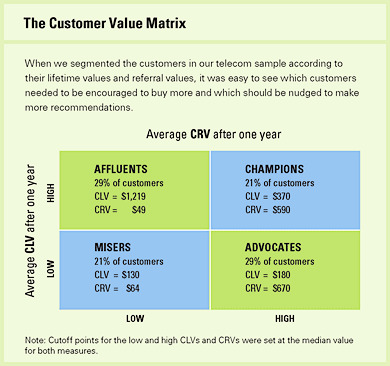
\includegraphics[width=5.42in]{images/customer_value_matrix} \end{center}

\hypertarget{finance-marketing-interface}{%
\chapter{Finance-Marketing Interface}\label{finance-marketing-interface}}

Market-based assets are: relational and intellectual.

Relational market-based assets are ``outcomes of the relationship between a firm and key external stakeholders, including distributors, retailers, end customers, other strategic partners''. \citep{Srivastava_1998}

For example, brand equity = relational assets between firms and their customers, while channel equity - relational assets between firms and their channel partners.

Intellectual market-based assets are ``the types of knowledge a firm possesses about the environment, such as the emerging and the potential state of market conditions and the entities in it, including competitors, customers, channels, suppliers, and social and political interest group.'' \citep{Srivastava_1998}

Marketing actions (e.g, adverting, product innovation) can build long-term assets (e.g., brand equity, customer equity), in turn increase short-term profitability (e.g., increase marketing effectiveness for dollars spent on advertising) \citep{Rust_2004}

\begin{center}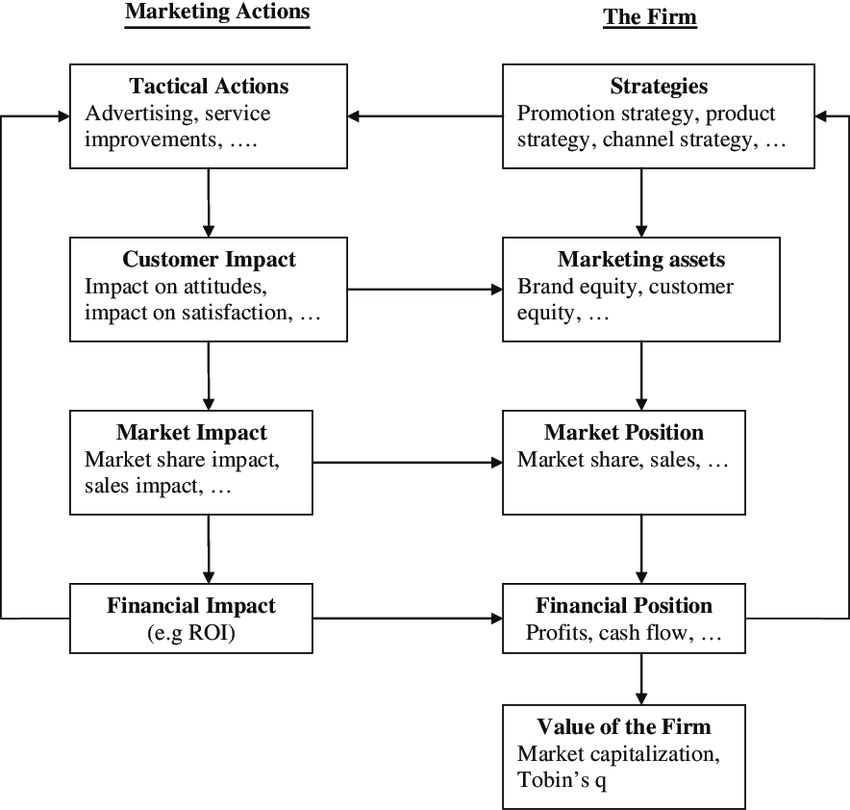
\includegraphics[width=11.81in]{images/The-chain-of-marketing-productivity-Source-Rust-et-al-2004} \end{center}

The Chain of Marketing Productivity (source \citep{Rust_2004})

Relationship between marketing and finance \citep{Srivastava_1998}

Stage 1: Market-based Assets

\begin{itemize}
\tightlist
\item
  Customer relationships: Brands, installed base.\\
\item
  Partner Relationship: channels, co-branding network.
\end{itemize}

Stage 2:

\begin{itemize}
\tightlist
\item
  Faster Market penetration\\
\item
  Price premium
\item
  share premium\\
\item
  extensions\\
\item
  reduce sales/service costs\\
\item
  Loyalty/ Retention
\end{itemize}

Stage 3: Shareholder value:

\begin{itemize}
\tightlist
\item
  Accelerate Cash Flows\\
\item
  Enhance Cash Flows\\
\item
  Reduce Volatility and Vulnerability of Cash flows\\
\item
  Enhance Residual Value of Cash Flows.
\end{itemize}

\citep{Grewal_2010, McAlister_2016, Morgan_2009} used Tobin's Q in marketing research. since it is ``forward-looking, risk-adjusted, and less easily manipulated by managers'' \citep{Wies_2019}. When probing factors affecting Tobin's Q, it was suggested to control for \protect\hyperlink{financial-leverage}{Financial Leverage},\protect\hyperlink{cash-flows}{Cash flows}

\hypertarget{tobins-q}{%
\section{Tobin's q}\label{tobins-q}}

Retrieve data from WRDS

\begin{Shaded}
\begin{Highlighting}[]
\CommentTok{# to set up connection from R to WRDS (https://wrds-www.wharton.upenn.edu/pages/support/programming-wrds/programming-r/r-from-your-computer/)}
\KeywordTok{library}\NormalTok{(RPostgres)}
\KeywordTok{library}\NormalTok{(dplyr)}

\CommentTok{# I've set up wrds connection before hand. Please use your username and password here.}

\CommentTok{# wrds <- dbConnect(Postgres(),}
\CommentTok{#                   host='wrds-pgdata.wharton.upenn.edu',}
\CommentTok{#                   port=9737,}
\CommentTok{#                   dbname='wrds',}
\CommentTok{#                   sslmode='require',}
\CommentTok{#                   user='')}

\CommentTok{# Check variables (column headers) in COMP ANNUAL FUNDAMENTAL}
\CommentTok{#uses the already-established wrds connection to prepare the SQL query string and save the query as the result res.}
\CommentTok{# check avaiable databases: https://wrds-web.wharton.upenn.edu/wrds/tools/variable.cfm?vendor_id=7}
\NormalTok{res <-}\StringTok{ }\KeywordTok{dbSendQuery}\NormalTok{(wrds, }\StringTok{"select column_name}
\StringTok{                   from information_schema.columns}
\StringTok{                   where table_schema='compa'}
\StringTok{                   and table_name='funda'}
\StringTok{                   order by column_name"}\NormalTok{)}
\NormalTok{data <-}\StringTok{ }\KeywordTok{dbFetch}\NormalTok{(res, }\DataTypeTok{n=}\OperatorTok{-}\DecValTok{1}\NormalTok{) }\CommentTok{# fetches the data that results from running the query res against wrds and stores it as data}
\KeywordTok{dbClearResult}\NormalTok{(res) }\CommentTok{# closes the connection}
\KeywordTok{head}\NormalTok{(data)}
\end{Highlighting}
\end{Shaded}

\begin{verbatim}
##   column_name
## 1       acchg
## 2        acco
## 3       accrt
## 4     acctchg
## 5     acctstd
## 6        acdo
\end{verbatim}

\begin{Shaded}
\begin{Highlighting}[]
\CommentTok{# select everything}
\NormalTok{res <-}\StringTok{ }\KeywordTok{dbSendQuery}\NormalTok{(wrds, }\StringTok{"select * from compa.funda"}\NormalTok{)}

\CommentTok{# from compa.funda}

\CommentTok{# only select the following variables}
\NormalTok{res <-}\StringTok{ }\KeywordTok{dbSendQuery}\NormalTok{(wrds, }\StringTok{"select gvkey, datadate, fyear, indfmt, consol, popsrc, datafmt, tic, cusip, conm, curcd, fyr, act, at, bkvlps, ceq, ch, che, dltt, dlc, emp, np, exchg, cik, costat, naicsh,mkvalt from compa.funda"}\NormalTok{) }\CommentTok{#check variables from (https://wrds-web.wharton.upenn.edu/wrds/ds/comp/funda/index.cfm?navId=80)}
\end{Highlighting}
\end{Shaded}

\begin{verbatim}
## Warning in result_create(conn@ptr, statement): Closing open result set,
## cancelling previous query
\end{verbatim}

\begin{Shaded}
\begin{Highlighting}[]
\NormalTok{data1 <-}\StringTok{ }\KeywordTok{dbFetch}\NormalTok{(res, }\DataTypeTok{n=}\OperatorTok{-}\DecValTok{1}\NormalTok{)}
\KeywordTok{dbClearResult}\NormalTok{(res)}

\NormalTok{data =}\StringTok{ }\NormalTok{data1 }\OperatorTok{%>%}
\StringTok{    }\KeywordTok{distinct}\NormalTok{(gvkey,datadate,fyear,tic,conm,}\DataTypeTok{.keep_all =}\NormalTok{ T)}
\end{Highlighting}
\end{Shaded}

Calculate Tobin's Q

\begin{Shaded}
\begin{Highlighting}[]
\NormalTok{tobin_q_dt =}\StringTok{ }\NormalTok{data }\OperatorTok{%>%}
\StringTok{    }\KeywordTok{mutate}\NormalTok{(}\DataTypeTok{mkvalt =} \KeywordTok{coalesce}\NormalTok{(mkvalt,}\DecValTok{0}\NormalTok{),}
           \DataTypeTok{dltt =} \KeywordTok{coalesce}\NormalTok{(dltt,}\DecValTok{0}\NormalTok{),}
           \DataTypeTok{at =} \KeywordTok{coalesce}\NormalTok{(at,}\DecValTok{0}\NormalTok{),}
           \DataTypeTok{dlc =} \KeywordTok{coalesce}\NormalTok{(dlc,}\DecValTok{0}\NormalTok{),}
           \DataTypeTok{act =} \KeywordTok{coalesce}\NormalTok{(act,}\DecValTok{0}\NormalTok{)) }\OperatorTok{%>%}
\StringTok{    }\KeywordTok{mutate}\NormalTok{(}\DataTypeTok{tobin_q =}\NormalTok{ (mkvalt }\OperatorTok{+}\StringTok{ }\KeywordTok{ifelse}\NormalTok{((dlc }\OperatorTok{-}\StringTok{ }\NormalTok{act) }\OperatorTok{>=}\DecValTok{0}\NormalTok{,}\KeywordTok{as.numeric}\NormalTok{(dlc}\OperatorTok{-}\NormalTok{act),}\DecValTok{0}\NormalTok{) }\OperatorTok{+}\StringTok{ }\NormalTok{dltt)}\OperatorTok{/}\NormalTok{at ) }\OperatorTok{%>%}\StringTok{  }\CommentTok{#follow Chung (1994) (sum of stocks (preferred + common) + debt(short-term liabilities - short-term assets + long-term debt))/(total assets) # note: take only excess of short-term liabilities over short-term assets to be included in debt. }
\StringTok{    }\KeywordTok{select}\NormalTok{(tobin_q,gvkey,datadate,fyear,conm)}
\KeywordTok{head}\NormalTok{(tobin_q_dt)}
\end{Highlighting}
\end{Shaded}

\begin{verbatim}
##     tobin_q  gvkey   datadate fyear                  conm
## 1       Inf 001000 1961-12-31  1961 A & E PLASTIK PAK INC
## 2       NaN 001000 1962-12-31  1962 A & E PLASTIK PAK INC
## 3       Inf 001000 1963-12-31  1963 A & E PLASTIK PAK INC
## 4 0.3686441 001000 1964-12-31  1964 A & E PLASTIK PAK INC
## 5 0.4995671 001000 1965-12-31  1965 A & E PLASTIK PAK INC
## 6 0.4563786 001000 1966-12-31  1966 A & E PLASTIK PAK INC
\end{verbatim}

\hypertarget{fama-and-french-three-factor-model}{%
\section{Fama and French Three-factor model}\label{fama-and-french-three-factor-model}}

\citep{Fama_1993}

An expansion from the capital asset pricing model (CAPM) to measure portfolio performance and future returns

Accounting for \textbf{company size}, and \textbf{value}

\[
R_{it} - R_{ft} = \alpha_{it} + \beta_1 (R_{Mt} - R_{ft}) + \beta_2 SMB_t + \beta_3 HML_t
\]
where

\begin{itemize}
\tightlist
\item
  \(R_{it}\) = total return of a stock or portfolio i at time t\\
\item
  \(R_{ft}\) = risk free rate of return at time t\\
\item
  \(R_{Mt}\) = total market portfolio return at time t\\
\item
  \(R_{it} - R_{ft}\) = expected excess return\\
\item
  \(R_{Mt} - R_{ft}\) = excess return on the market portfolio (index)\\
\item
  \(SMB_t\) = size premium (small - big)\\
\item
  \(HML_t\) = value premium (high - low), also known as value premum (i.e., companies with high book-to-market stocks are called value stocks)
\item
  \(\beta_{1,2,3}\) = factor coefficients
\end{itemize}

\hypertarget{example-1}{%
\subsection{Example 1}\label{example-1}}

Example from \href{http://www.calculatinginvestor.com/2011/04/19/fama-french-tutorial/}{Calculating Investor}

\begin{Shaded}
\begin{Highlighting}[]
\CommentTok{# Fama-French Regression example in R}

\CommentTok{#download factors from https://mba.tuck.dartmouth.edu/pages/faculty/ken.french/data_library.html}

\CommentTok{# Load CSV file into R }
\NormalTok{ff_data <-}\StringTok{ }\KeywordTok{read.table}\NormalTok{(}\StringTok{"images/ffdata.csv"}\NormalTok{,}\DataTypeTok{header=}\OtherTok{TRUE}\NormalTok{,}\DataTypeTok{sep=}\StringTok{","}\NormalTok{)}
 
\CommentTok{# Extract Fama-French Factors and Fund Returns}
\NormalTok{rmrf <-}\StringTok{ }\NormalTok{ff_data[,}\DecValTok{2}\NormalTok{]}\OperatorTok{/}\DecValTok{100}
\NormalTok{smb <-}\StringTok{ }\NormalTok{ff_data[,}\DecValTok{3}\NormalTok{]}\OperatorTok{/}\DecValTok{100}
\NormalTok{hml <-}\StringTok{ }\NormalTok{ff_data[,}\DecValTok{4}\NormalTok{]}\OperatorTok{/}\DecValTok{100}
\NormalTok{rf <-}\StringTok{ }\NormalTok{ff_data[,}\DecValTok{5}\NormalTok{]}\OperatorTok{/}\DecValTok{100}
\NormalTok{fund <-}\StringTok{ }\NormalTok{ff_data[,}\DecValTok{6}\NormalTok{]}\OperatorTok{/}\DecValTok{100}
 
\CommentTok{# Calculate Excess Returns for Target fund}
\NormalTok{fund.xcess <-}\StringTok{ }\NormalTok{fund }\OperatorTok{-}\StringTok{ }\NormalTok{rf}
 
\CommentTok{# Run Fama-French Regression}
\NormalTok{ffregression <-}\StringTok{ }\KeywordTok{lm}\NormalTok{(fund.xcess }\OperatorTok{~}\StringTok{ }\NormalTok{rmrf }\OperatorTok{+}\StringTok{ }\NormalTok{smb }\OperatorTok{+}\StringTok{ }\NormalTok{hml)}
 
\CommentTok{# Print summary of regression results}
\KeywordTok{print}\NormalTok{(}\KeywordTok{summary}\NormalTok{(ffregression))}
\end{Highlighting}
\end{Shaded}

\begin{verbatim}
## 
## Call:
## lm(formula = fund.xcess ~ rmrf + smb + hml)
## 
## Residuals:
##       Min        1Q    Median        3Q       Max 
## -0.043944 -0.008162 -0.000333  0.009172  0.042174 
## 
## Coefficients:
##              Estimate Std. Error t value Pr(>|t|)    
## (Intercept) -0.002922   0.001946  -1.502  0.13881    
## rmrf         1.210644   0.041743  29.002  < 2e-16 ***
## smb          0.151090   0.086468   1.747  0.08606 .  
## hml         -0.298928   0.073488  -4.068  0.00015 ***
## ---
## Signif. codes:  0 '***' 0.001 '**' 0.01 '*' 0.05 '.' 0.1 ' ' 1
## 
## Residual standard error: 0.01491 on 56 degrees of freedom
## Multiple R-squared:  0.9509, Adjusted R-squared:  0.9483 
## F-statistic: 361.7 on 3 and 56 DF,  p-value: < 2.2e-16
\end{verbatim}

This is monthly data, and we can see \(\alpha\) term is negative means that the portfolio underperformed compared to the market.

\hypertarget{example-2}{%
\subsection{Example 2}\label{example-2}}

Example from \href{https://rviews.rstudio.com/2018/04/11/introduction-to-fama-french/}{R View}

\begin{Shaded}
\begin{Highlighting}[]
\KeywordTok{library}\NormalTok{(tidyquant)}
\KeywordTok{library}\NormalTok{(tidyverse)}
\KeywordTok{library}\NormalTok{(timetk)}
\KeywordTok{library}\NormalTok{(broom)}
\KeywordTok{library}\NormalTok{(glue)}

\NormalTok{symbols <-}\StringTok{ }\KeywordTok{c}\NormalTok{(}\StringTok{"SPY"}\NormalTok{,}\StringTok{"EFA"}\NormalTok{, }\StringTok{"IJS"}\NormalTok{, }\StringTok{"EEM"}\NormalTok{,}\StringTok{"AGG"}\NormalTok{)}



\NormalTok{prices <-}\StringTok{ }
\StringTok{  }\KeywordTok{getSymbols}\NormalTok{(symbols, }\DataTypeTok{src =} \StringTok{'yahoo'}\NormalTok{, }
             \DataTypeTok{from =} \StringTok{"2012-12-31"}\NormalTok{,}
             \DataTypeTok{to =} \StringTok{"2017-12-31"}\NormalTok{,}
             \DataTypeTok{auto.assign =} \OtherTok{TRUE}\NormalTok{, }\DataTypeTok{warnings =} \OtherTok{FALSE}\NormalTok{) }\OperatorTok{%>%}\StringTok{ }
\StringTok{  }\KeywordTok{map}\NormalTok{(}\OperatorTok{~}\KeywordTok{Ad}\NormalTok{(}\KeywordTok{get}\NormalTok{(.))) }\OperatorTok{%>%}
\StringTok{  }\KeywordTok{reduce}\NormalTok{(merge) }\OperatorTok{%>%}\StringTok{ }
\StringTok{  `}\DataTypeTok{colnames<-}\StringTok{`}\NormalTok{(symbols)}

\NormalTok{w <-}\StringTok{ }\KeywordTok{c}\NormalTok{(}\FloatTok{0.25}\NormalTok{, }\FloatTok{0.25}\NormalTok{, }\FloatTok{0.20}\NormalTok{, }\FloatTok{0.20}\NormalTok{, }\FloatTok{0.10}\NormalTok{)}

\CommentTok{# + SPY (S&P500 fund) weighted 25%}
\CommentTok{# + EFA (a non-US equities fund) weighted 25%}
\CommentTok{# + IJS (a small-cap value fund) weighted 20%}
\CommentTok{# + EEM (an emerging-mkts fund) weighted 20%}
\CommentTok{# + AGG (a bond fund) weighted 10%}

\NormalTok{asset_returns_long <-}\StringTok{  }
\StringTok{  }\NormalTok{prices }\OperatorTok{%>%}\StringTok{ }
\StringTok{  }\KeywordTok{to.monthly}\NormalTok{(}\DataTypeTok{indexAt =} \StringTok{"lastof"}\NormalTok{, }\DataTypeTok{OHLC =} \OtherTok{FALSE}\NormalTok{) }\OperatorTok{%>%}\StringTok{ }
\StringTok{  }\KeywordTok{tk_tbl}\NormalTok{(}\DataTypeTok{preserve_index =} \OtherTok{TRUE}\NormalTok{, }\DataTypeTok{rename_index =} \StringTok{"date"}\NormalTok{) }\OperatorTok{%>%}
\StringTok{  }\KeywordTok{gather}\NormalTok{(asset, returns, }\OperatorTok{-}\NormalTok{date) }\OperatorTok{%>%}\StringTok{ }
\StringTok{  }\KeywordTok{group_by}\NormalTok{(asset) }\OperatorTok{%>%}\StringTok{  }
\StringTok{  }\KeywordTok{mutate}\NormalTok{(}\DataTypeTok{returns =}\NormalTok{ (}\KeywordTok{log}\NormalTok{(returns) }\OperatorTok{-}\StringTok{ }\KeywordTok{log}\NormalTok{(}\KeywordTok{lag}\NormalTok{(returns)))) }\OperatorTok{%>%}\StringTok{ }
\StringTok{  }\KeywordTok{na.omit}\NormalTok{()}

\NormalTok{portfolio_returns_tq_rebalanced_monthly <-}\StringTok{ }
\StringTok{  }\NormalTok{asset_returns_long }\OperatorTok{%>%}
\StringTok{  }\KeywordTok{tq_portfolio}\NormalTok{(}\DataTypeTok{assets_col  =}\NormalTok{ asset, }
               \DataTypeTok{returns_col =}\NormalTok{ returns,}
               \DataTypeTok{weights     =}\NormalTok{ w,}
               \DataTypeTok{col_rename  =} \StringTok{"returns"}\NormalTok{,}
               \DataTypeTok{rebalance_on =} \StringTok{"months"}\NormalTok{)}
\end{Highlighting}
\end{Shaded}

\begin{Shaded}
\begin{Highlighting}[]
\NormalTok{temp <-}\StringTok{ }\KeywordTok{tempfile}\NormalTok{()}

\NormalTok{base <-}\StringTok{ "http://mba.tuck.dartmouth.edu/pages/faculty/ken.french/ftp/"}

\NormalTok{factor <-}\StringTok{  "Global_3_Factors"}

\NormalTok{format<-}\StringTok{ "_CSV.zip"}

\NormalTok{full_url <-}\StringTok{ }\KeywordTok{glue}\NormalTok{(base,}
\NormalTok{                 factor,}
\NormalTok{                 format,}
                 \DataTypeTok{sep =} \StringTok{""}\NormalTok{)}

\KeywordTok{download.file}\NormalTok{(full_url,}
\NormalTok{              temp,}
              \DataTypeTok{quiet =} \OtherTok{TRUE}\NormalTok{)}


\CommentTok{# Global_3_Factors <-}
\CommentTok{#   read_csv(unz(temp,}
\CommentTok{#                "Global_3_Factors.csv"))}
\CommentTok{# }
\CommentTok{# head(Global_3_Factors)  }

\CommentTok{# skip 6 rows so we can have the right format}
\NormalTok{Global_}\DecValTok{3}\NormalTok{_Factors <-}\StringTok{ }
\StringTok{  }\KeywordTok{read_csv}\NormalTok{(}\KeywordTok{unz}\NormalTok{(temp, }
               \StringTok{"Global_3_Factors.csv"}\NormalTok{), }
    \DataTypeTok{skip =} \DecValTok{6}\NormalTok{)}
\end{Highlighting}
\end{Shaded}

\begin{verbatim}
## Warning: Missing column names filled in: 'X1' [1]
\end{verbatim}

\begin{verbatim}
## Warning: 1 parsing failure.
## row col  expected    actual         file
## 349  -- 5 columns 1 columns <connection>
\end{verbatim}

\begin{Shaded}
\begin{Highlighting}[]
\KeywordTok{head}\NormalTok{(Global_}\DecValTok{3}\NormalTok{_Factors)}
\end{Highlighting}
\end{Shaded}

\begin{verbatim}
## # A tibble: 6 x 5
##   X1     `Mkt-RF` SMB   HML   RF   
##   <chr>  <chr>    <chr> <chr> <chr>
## 1 199007 0.77     0.55  -0.40 0.68 
## 2 199008 -10.77   -1.49 0.53  0.66 
## 3 199009 -11.88   1.35  0.71  0.60 
## 4 199010 9.36     -7.57 -4.16 0.68 
## 5 199011 -3.72    1.37  1.13  0.57 
## 6 199012 1.11     -0.72 -1.52 0.60
\end{verbatim}

\begin{Shaded}
\begin{Highlighting}[]
\CommentTok{# X1 = formatted dates}
\CommentTok{# Mkt-Rf for the market returns above the risk-free rate}
\CommentTok{# SMB for the size factor}
\CommentTok{# HML for the value factor}
\CommentTok{# RF for the risk-free rate}

\CommentTok{#check data type}
\KeywordTok{map}\NormalTok{(Global_}\DecValTok{3}\NormalTok{_Factors, class)}
\end{Highlighting}
\end{Shaded}

\begin{verbatim}
## $X1
## [1] "character"
## 
## $`Mkt-RF`
## [1] "character"
## 
## $SMB
## [1] "character"
## 
## $HML
## [1] "character"
## 
## $RF
## [1] "character"
\end{verbatim}

\begin{Shaded}
\begin{Highlighting}[]
\NormalTok{Global_}\DecValTok{3}\NormalTok{_Factors <-}
\StringTok{  }\KeywordTok{read_csv}\NormalTok{(}\KeywordTok{unz}\NormalTok{(temp,}
               \StringTok{"Global_3_Factors.csv"}\NormalTok{),}
           \DataTypeTok{skip =} \DecValTok{6}\NormalTok{) }\OperatorTok{%>%}
\StringTok{  }\KeywordTok{rename}\NormalTok{(}\DataTypeTok{date =}\NormalTok{ X1) }\OperatorTok{%>%}
\StringTok{  }\KeywordTok{mutate_at}\NormalTok{(}\KeywordTok{vars}\NormalTok{(}\OperatorTok{-}\NormalTok{date), as.numeric) }\OperatorTok{%>%}
\StringTok{  }\KeywordTok{mutate}\NormalTok{(}\DataTypeTok{date =}
           \KeywordTok{rollback}\NormalTok{(}\KeywordTok{ymd}\NormalTok{(}\KeywordTok{parse_date_time}\NormalTok{(date, }\StringTok{"%Y%m"}\NormalTok{) }\OperatorTok{+}\StringTok{ }\KeywordTok{months}\NormalTok{(}\DecValTok{1}\NormalTok{)))) }\OperatorTok{%>%}
\StringTok{  }\KeywordTok{filter}\NormalTok{(}
\NormalTok{    date }\OperatorTok{>=}
\StringTok{      }\KeywordTok{first}\NormalTok{(portfolio_returns_tq_rebalanced_monthly}\OperatorTok{$}\NormalTok{date) }\OperatorTok{&}\StringTok{ }\NormalTok{date }\OperatorTok{<=}
\StringTok{      }\KeywordTok{last}\NormalTok{(portfolio_returns_tq_rebalanced_monthly}\OperatorTok{$}\NormalTok{date)}
\NormalTok{  )}
\end{Highlighting}
\end{Shaded}

\begin{verbatim}
## Warning: Missing column names filled in: 'X1' [1]

## Warning: 1 parsing failure.
## row col  expected    actual         file
## 349  -- 5 columns 1 columns <connection>
\end{verbatim}

\begin{verbatim}
## Warning in mask$eval_all_mutate(quo): NAs introduced by coercion

## Warning in mask$eval_all_mutate(quo): NAs introduced by coercion

## Warning in mask$eval_all_mutate(quo): NAs introduced by coercion

## Warning in mask$eval_all_mutate(quo): NAs introduced by coercion
\end{verbatim}

\begin{verbatim}
## Warning: 29 failed to parse.
\end{verbatim}

\begin{Shaded}
\begin{Highlighting}[]
\KeywordTok{head}\NormalTok{(Global_}\DecValTok{3}\NormalTok{_Factors)}
\end{Highlighting}
\end{Shaded}

\begin{verbatim}
## # A tibble: 6 x 5
##   date       `Mkt-RF`   SMB   HML    RF
##   <date>        <dbl> <dbl> <dbl> <dbl>
## 1 2013-01-31     5.46  0.17  2.01     0
## 2 2013-02-28     0.09  0.35 -0.76     0
## 3 2013-03-31     2.29  0.85 -2.02     0
## 4 2013-04-30     3.02 -1.13  0.9      0
## 5 2013-05-31     0.56 -0.66  0.97     0
## 6 2013-06-30    -2.52  0.21 -0.06     0
\end{verbatim}

\hypertarget{carhart-four-factor-model}{%
\section{Carhart Four-factor model}\label{carhart-four-factor-model}}

\citep{Carhart_1997}

\[
R_{it} - R_{ft} = \alpha_{it} + \beta_1 (R_{Mt} - R_{ft}) + \beta_2 SMB_t + \beta_3 HML_t + \beta_4 UMD_t
\]
where

\begin{itemize}
\tightlist
\item
  \(R_{it}\) = total return of a stock or portfolio i at time t\\
\item
  \(R_{ft}\) = risk free rate of return at time t\\
\item
  \(R_{Mt}\) = total market portfolio return at time t\\
\item
  \(R_{it} - R_{ft}\) = expected excess return\\
\item
  \(R_{Mt} - R_{ft}\) = excess return on the market portfolio (index)\\
\item
  \(SMB_t\) = size premium (small - big)\\
\item
  \(HML_t\) = value premium (high - low)\\
\item
  \(UMD_t\) = premium on winners minus losers.\\
\item
  \(\beta_{1,2,3}\) = factor coefficients
\end{itemize}

\hypertarget{fama-and-french-five-factor-model}{%
\section{Fama and French Five-factor model}\label{fama-and-french-five-factor-model}}

\citep{Fama_2015}
Accounting additionally for profitability and investment factors

\[
R_{it} - R_{ft} = \alpha_{it} + \beta_1 (R_{Mt} - R_{ft}) + \beta_2 SMB_t + \beta_3 HML_t + \beta_4 RMW_t + \beta_5 CMA_t + e_{it}
\]
where

\begin{itemize}
\tightlist
\item
  \(R_{it}\) = total return of a stock or portfolio i at time t\\
\item
  \(R_{ft}\) = risk free rate of return at time t\\
\item
  \(R_{Mt}\) = total market portfolio return at time t\\
\item
  \(R_{it} - R_{ft}\) = expected excess return\\
\item
  \(R_{Mt} - R_{ft}\) = excess return on the market portfolio (index)\\
\item
  \(SMB_t\) = size premium (small - big)\\
\item
  \(HML_t\) = value premium (high - low)\\
\item
  \(\beta_{1,2,3}\) = factor coefficients\\
\item
  \(RMW_t\) is the return spread of the most profitable firms - the least profitable\\
\item
  \(CMA_t\) is the return spread of firms that invest conservatively minus aggressively .
\end{itemize}

\hypertarget{multi-factor-model}{%
\section{Multi-Factor Model}\label{multi-factor-model}}

\[
R_i = \alpha_i + \beta_{i(m)} Rm + \beta_{i(1)} F_1 + ...+ \beta_{i(n)} F_n + \epsilon_i
\]

where

\begin{itemize}
\tightlist
\item
  \(R_i\) = return of security\\
\item
  \(Rm\) = market return\\
\item
  \(F(1,...N)\) = factors used
\end{itemize}

Factors can be

\begin{itemize}
\tightlist
\item
  Macroeconomic: employment, inflation, interest.\\
\item
  Fundamental: (underlying financials): earnings, market cap, debt levels.\\
\item
  Statistical: historical data modeling.
\end{itemize}

Type of Multi-Factor Models

\begin{itemize}
\tightlist
\item
  Bomicnaiton mdoel:
\end{itemize}

\hypertarget{event-study}{%
\section{Event study}\label{event-study}}

\hypertarget{abnormal-return}{%
\subsection{Abnormal Return}\label{abnormal-return}}

\url{https://rpubs.com/gregoryarobinson/315096}

\url{https://www.eventstudytools.com/introduction-event-study-methodology}

\begin{Shaded}
\begin{Highlighting}[]
\CommentTok{# install.packages("EventStudy")}
\KeywordTok{library}\NormalTok{(EventStudy)}
\end{Highlighting}
\end{Shaded}

Another package

\url{https://cran.r-project.org/web/packages/eventstudies/vignettes/replications.pdf}

\begin{Shaded}
\begin{Highlighting}[]
\KeywordTok{library}\NormalTok{(eventstudies)}
\end{Highlighting}
\end{Shaded}

Replication of \citep{Chen_2004}

\begin{Shaded}
\begin{Highlighting}[]
\KeywordTok{data}\NormalTok{(TerrorIndiceReturns)}
\KeywordTok{data}\NormalTok{(TerrorAttack)}
\NormalTok{TerrorIndiceCAR <-}\StringTok{ }\KeywordTok{lapply}\NormalTok{(}\DecValTok{1}\OperatorTok{:}\StringTok{ }\KeywordTok{ncol}\NormalTok{(TerrorIndiceReturns), }\ControlFlowTok{function}\NormalTok{(x)\{}
\CommentTok{# 10-day window around the event}
\NormalTok{event <-}\StringTok{ }\KeywordTok{phys2eventtime}\NormalTok{(}\KeywordTok{na.omit}\NormalTok{(TerrorIndiceReturns[ , x,}
\DataTypeTok{drop =} \OtherTok{FALSE}\NormalTok{]),}
\NormalTok{TerrorAttack,}
\DecValTok{10}\NormalTok{)}
\CommentTok{# Estimate ARs}
\NormalTok{esMean <-}\StringTok{ }\KeywordTok{constantMeanReturn}\NormalTok{(event}\OperatorTok{$}\NormalTok{z.e[}\KeywordTok{which}\NormalTok{(}\KeywordTok{attributes}\NormalTok{(event}\OperatorTok{$}\NormalTok{z.e)}\OperatorTok{$}\NormalTok{index}
\OperatorTok{%in%}\StringTok{ }\DecValTok{-30}\OperatorTok{:-}\DecValTok{11}\NormalTok{), ],}
\DataTypeTok{residual =} \OtherTok{FALSE}\NormalTok{)}
\NormalTok{ar <-}\StringTok{ }\NormalTok{event}\OperatorTok{$}\NormalTok{z.e }\OperatorTok{-}\StringTok{ }\NormalTok{esMean}
\NormalTok{ar <-}\StringTok{ }\KeywordTok{window}\NormalTok{(ar, }\DataTypeTok{start =} \DecValTok{0}\NormalTok{, }\DataTypeTok{end =} \DecValTok{10}\NormalTok{)}
\CommentTok{# CAR}
\NormalTok{car <-}\StringTok{ }\KeywordTok{remap.cumsum}\NormalTok{(ar, }\DataTypeTok{base =} \KeywordTok{as.numeric}\NormalTok{(ar[}\DecValTok{1}\NormalTok{, }\DecValTok{1}\NormalTok{]))}
\KeywordTok{names}\NormalTok{(car) <-}\StringTok{ }\KeywordTok{colnames}\NormalTok{(TerrorIndiceReturns[ , x,}
\DataTypeTok{drop =} \OtherTok{FALSE}\NormalTok{])}
\KeywordTok{return}\NormalTok{(car)}
\NormalTok{\})}
\KeywordTok{names}\NormalTok{(TerrorIndiceCAR) <-}\StringTok{ }\KeywordTok{colnames}\NormalTok{(TerrorIndiceReturns)}
\CommentTok{# Compile for all indices}
\NormalTok{TerrorIndiceCAR <-}\StringTok{ }\KeywordTok{do.call}\NormalTok{(cbind, TerrorIndiceCAR)}
\CommentTok{# 11-day CAR}
\NormalTok{TerrorIndiceCAR[}\DecValTok{11}\NormalTok{, ]}
\end{Highlighting}
\end{Shaded}

\begin{verbatim}
##       S.P500       Dow      NYSE    NASDAQ   Toronto   Mexico    London
## 10 -3.832794 -7.897366 -3.981837 -9.993519 -9.110412 -6.53973 -8.602633
##      Germany Eurostoxx50    France    Spain Switzerland   Austria     Italy
## 10 -10.45718   -7.596024 -9.518721 -10.6724   -7.292201 -7.894399 -15.21462
##      Belgium Amsterdam Portugal  Helsinki    Norway    Sweden     Tokyo
## 10 -9.219016 -10.82756 1.698079 -5.500048 -12.39281 -4.691903 -3.603373
##     HongKong   S.Korea     India   Jakarta Singapore Kualalampur Australia
## 10 -5.231521 -16.64571 -17.02777 -9.933654 -17.98219   -14.55417 -8.597988
##          NZL  Pakistan     Saudi   Israel     Jberg
## 10 -5.635766 -12.42189 -11.32466 -7.81159 -12.59022
\end{verbatim}

\begin{Shaded}
\begin{Highlighting}[]
\NormalTok{TerrorIndiceCAR[}\DecValTok{6}\NormalTok{, ] }\CommentTok{# 6-day CAR}
\end{Highlighting}
\end{Shaded}

\begin{verbatim}
##     S.P500       Dow      NYSE    NASDAQ  Toronto    Mexico    London   Germany
## 5 -7.72379 -10.56695 -8.094739 -10.13781 -7.01292 -13.17444 -4.533527 -8.063819
##   Eurostoxx50    France     Spain Switzerland   Austria     Italy   Belgium
## 5   -5.940704 -8.707865 -9.426443   -5.967055 -4.428614 -13.98185 -8.510382
##   Amsterdam  Portugal  Helsinki    Norway   Sweden      Tokyo  HongKong
## 5 -8.521101 -6.875878 -4.802975 -9.894391 -4.96208 -0.5636291 -5.570385
##     S.Korea     India  Jakarta Singapore Kualalampur Australia       NZL
## 5 -11.81901 -11.77841 -4.91951 -13.74157   -10.50214 -6.814062 -7.101218
##   Pakistan     Saudi    Israel     Jberg
## 5 -10.3741 -5.320904 -11.03399 -12.09548
\end{verbatim}

\hypertarget{advertising-1}{%
\chapter{Advertising}\label{advertising-1}}

People don't like intrusive ads, especially when they are vulnerable \citep[p.143]{kellogg_2005}

\hypertarget{metrics}{%
\chapter{Metrics}\label{metrics}}

\hypertarget{return-on-investment-roi}{%
\section{Return on Investment (ROI)}\label{return-on-investment-roi}}

\[
ROI = \frac{\text{Net Profit}}{\text{Investment}}
\]

Similarly, return on marketing investment

\[
ROIM = \frac{IRAM - CM}{MS}
\]

where

\begin{itemize}
\tightlist
\item
  IRAM = Incremental Revenue Attributable to Marketing\\
\item
  CM = Cost of the Marketing Investment\\
\item
  MS = Marketing Spending
\end{itemize}

If ROMI is positive, then firm is on doing well.

\hypertarget{economic-value-added}{%
\section{Economic Value Added}\label{economic-value-added}}

\begin{itemize}
\tightlist
\item
  also known as economic profit.\\
\item
  is a measure based on the residual wealth calculated by deducting its cost of capital from its operating profit, adjusted for taxes on a cash basis.\\
\item
  measures the value a company generates from its invested funds.\\
\item
  EVA relies heavily on invested capital. Hence, more suitable for asset-rich companies, whereas companies with intangible assets, such as technology businesses, may not be good candidates.
\end{itemize}

\[
EVA = NOPAT - (Invested Capital * WACC)
\]

where

\begin{itemize}
\tightlist
\item
  NOPAT = Net Operating profit after taxes = Operating Profit x (1-Tax Rate)\\
\item
  Invested capital = Debt + capital leases + shareholders' equity = Equity + long-term debt at the beginning of the period\\
\item
  WACC = Weighted average cost of capital (average rate of return a company expects to pay its investors).

  \begin{itemize}
  \tightlist
  \item
    \(WACC = \frac{Ke \times E}{E+D} + \frac{Kd \times (1-t) \times D}{E +D }\)

    \begin{itemize}
    \tightlist
    \item
      Ke = required return on equity\\
    \item
      Kd(1-t) = after tax return on debt.\\
    \end{itemize}
  \end{itemize}
\item
  (WACC* capital invested) is also known as a \textbf{finance charge}
\end{itemize}

Invested capital can also be calculated as (Total Assets - Current Liabilities). Hence, the modified version of EVA is:

\[
EVA = NOPAT - (\text{total assets} - \text{current liabilities}) * WACC
\]

\hypertarget{market-value-added}{%
\section{Market Value Added}\label{market-value-added}}

\begin{itemize}
\tightlist
\item
  is the amount of wealth that a company is able to create for its stakeholders since its foundation.\\
\item
  (the current market value of the company's stock - the initial invested capital)
\end{itemize}

\[
MVA = \text{market value of shares (or enterprise value)} - \text{book value of shareholders' equity}
\]

\hypertarget{unexpected-size-adjusted-advertising-investments}{%
\section{Unexpected size-adjusted advertising investments}\label{unexpected-size-adjusted-advertising-investments}}

\citep{Chakravarty_2016, Kim_2011, Liu_2017} used

\hypertarget{shareholder-complaints}{%
\section{Shareholder Complaints}\label{shareholder-complaints}}

\citep{Wies_2019} used data from RiskMetrics

\hypertarget{profitability}{%
\section{Profitability}\label{profitability}}

\citep{Grewal_2008, McAlister_2016}

\[
\text{profitability} = \frac{\text{operating income before depreciation}}{\text{total assets}}
\]

\hypertarget{firm-size}{%
\section{Firm Size}\label{firm-size}}

\citep{Grewal_2010, McAlister_2016, Nezami_2018} used log of total asset in million as firm size

\[
\text{firm size} = \log (\text{total assets})
\]
\#\# Sales Growth
\citep{Grewal_2010, Nezami_2018, Rao_2004}

Percentage change in gross sales = sales growth

\hypertarget{financial-flexibility}{%
\section{Financial Flexibility}\label{financial-flexibility}}

\hypertarget{cash-flows}{%
\subsection{Cash flows}\label{cash-flows}}

\citep{Chakravarty_2011, Malshe_2015}
Cash flows = log(operating cash flow in mil)

\hypertarget{financial-leverage}{%
\subsection{Financial Leverage}\label{financial-leverage}}

\citep{Kashmiri_2017, Chakravarty_2011}

\[
\text{financial leverage} = \frac{\text{long-term debt}}{\text{book value of assets}}
\]

\hypertarget{stock-return}{%
\section{Stock return}\label{stock-return}}

\citep{Markovitch_2005, Chakravarty_2011, Chakravarty_2016} used dummy if stock returns exceed industry averaged stock returns

\hypertarget{financial-flexibility-1}{%
\section{Financial Flexibility}\label{financial-flexibility-1}}

\hypertarget{net-contribution}{%
\section{Net Contribution}\label{net-contribution}}

Net contribution = gross margin x sales - cost of marketing

\[
NC = m \times S(a) -ka
\]

\hypertarget{data}{%
\chapter{Data}\label{data}}

\hypertarget{wrds}{%
\section{WRDS}\label{wrds}}

Retrieve data from WRDS

\begin{Shaded}
\begin{Highlighting}[]
\CommentTok{# to set up connection from R to WRDS (https://wrds-www.wharton.upenn.edu/pages/support/programming-wrds/programming-r/r-from-your-computer/)}
\KeywordTok{library}\NormalTok{(RPostgres)}
\KeywordTok{library}\NormalTok{(dplyr)}

\CommentTok{# I've set up wrds connection before hand. Please use your username and password here.}

\CommentTok{# wrds <- dbConnect(Postgres(),}
\CommentTok{#                   host='wrds-pgdata.wharton.upenn.edu',}
\CommentTok{#                   port=9737,}
\CommentTok{#                   dbname='wrds',}
\CommentTok{#                   sslmode='require',}
\CommentTok{#                   user='')}

\CommentTok{# Check variables (column headers) in COMP ANNUAL FUNDAMENTAL}
\CommentTok{#uses the already-established wrds connection to prepare the SQL query string and save the query as the result res.}
\CommentTok{# check avaiable databases: https://wrds-web.wharton.upenn.edu/wrds/tools/variable.cfm?vendor_id=7}
\NormalTok{res <-}\StringTok{ }\KeywordTok{dbSendQuery}\NormalTok{(wrds, }\StringTok{"select column_name}
\StringTok{                   from information_schema.columns}
\StringTok{                   where table_schema='compa'}
\StringTok{                   and table_name='funda'}
\StringTok{                   order by column_name"}\NormalTok{)}
\NormalTok{data <-}\StringTok{ }\KeywordTok{dbFetch}\NormalTok{(res, }\DataTypeTok{n=}\OperatorTok{-}\DecValTok{1}\NormalTok{) }\CommentTok{# fetches the data that results from running the query res against wrds and stores it as data}
\KeywordTok{dbClearResult}\NormalTok{(res) }\CommentTok{# closes the connection}
\KeywordTok{head}\NormalTok{(data)}
\end{Highlighting}
\end{Shaded}

\begin{verbatim}
##   column_name
## 1       acchg
## 2        acco
## 3       accrt
## 4     acctchg
## 5     acctstd
## 6        acdo
\end{verbatim}

\begin{Shaded}
\begin{Highlighting}[]
\CommentTok{# select everything}
\NormalTok{res <-}\StringTok{ }\KeywordTok{dbSendQuery}\NormalTok{(wrds, }\StringTok{"select * from compa.funda"}\NormalTok{)}

\CommentTok{# from compa.funda}

\CommentTok{# only select the following variables}
\NormalTok{res <-}\StringTok{ }\KeywordTok{dbSendQuery}\NormalTok{(wrds, }\StringTok{"select gvkey, datadate, fyear, indfmt, consol, popsrc, datafmt, tic, cusip, conm, curcd, fyr, act, at, bkvlps, ceq, ch, che, dltt, dlc, emp, np, exchg, cik, costat, naicsh,mkvalt from compa.funda"}\NormalTok{) }\CommentTok{#check variables from (https://wrds-web.wharton.upenn.edu/wrds/ds/comp/funda/index.cfm?navId=80)}
\end{Highlighting}
\end{Shaded}

\begin{verbatim}
## Warning in result_create(conn@ptr, statement): Closing open result set,
## cancelling previous query
\end{verbatim}

\begin{Shaded}
\begin{Highlighting}[]
\CommentTok{# res <- dbSendQuery(wrds, "select gvkey, gp from compa.funda") #check variables from}
\NormalTok{data1 <-}\StringTok{ }\KeywordTok{dbFetch}\NormalTok{(res, }\DataTypeTok{n=}\OperatorTok{-}\DecValTok{1}\NormalTok{)}
\KeywordTok{dbClearResult}\NormalTok{(res)}

\NormalTok{data =}\StringTok{ }\NormalTok{data1 }\OperatorTok{%>%}
\StringTok{    }\KeywordTok{distinct}\NormalTok{(gvkey,datadate,fyear,tic,conm,}\DataTypeTok{.keep_all =}\NormalTok{ T)}
\end{Highlighting}
\end{Shaded}

\hypertarget{youtube}{%
\section{YouTube}\label{youtube}}

\begin{itemize}
\tightlist
\item
  \href{https://www.youtube.com/intl/en_us/ads/how-it-works/measure-your-results/}{YouTube Ads}\\
\item
  \href{https://developers.google.com/youtube/reporting}{YouTube Analytics and Reporting APIs}: All YouTube Analytics and YouTube Reporting API requests must be authorized by the channel or content owner that owns the requested data
\end{itemize}

\hypertarget{oauth}{%
\subsection{OAuth}\label{oauth}}

Go to \href{https://console.cloud.google.com/apis/api/youtube.googleapis.com}{link} to access your API

\begin{Shaded}
\begin{Highlighting}[]
\KeywordTok{library}\NormalTok{(tuber)}
\NormalTok{app_id =}\StringTok{ "YOUR APP ID"}
\NormalTok{app_secret =}\StringTok{ "YOUR APP SECRET"}
\KeywordTok{yt_oauth}\NormalTok{(app_id, app_secret)}


\KeywordTok{get_stats}\NormalTok{(}\DataTypeTok{video_id =} \StringTok{"N708P-A45D0"}\NormalTok{)}
\end{Highlighting}
\end{Shaded}

Note for Ubuntu user

\begin{Shaded}
\begin{Highlighting}[]
\NormalTok{httr}\OperatorTok{::}\KeywordTok{set_config}\NormalTok{(httr}\OperatorTok{::}\KeywordTok{config}\NormalTok{( }\DataTypeTok{ssl_verifypeer =}\NormalTok{ 0L ) )}
\end{Highlighting}
\end{Shaded}

Get info about a video

\begin{Shaded}
\begin{Highlighting}[]
\KeywordTok{get_video_details}\NormalTok{(}\DataTypeTok{video_id=}\StringTok{"N708P-A45D0"}\NormalTok{)}
\end{Highlighting}
\end{Shaded}

Get caption of a video

\begin{Shaded}
\begin{Highlighting}[]
\KeywordTok{get_captions}\NormalTok{(}\DataTypeTok{video_id=}\StringTok{"yJXTXN4xrI8"}\NormalTok{)}
\end{Highlighting}
\end{Shaded}

Search Videos

\begin{Shaded}
\begin{Highlighting}[]
\NormalTok{res <-}\StringTok{ }\KeywordTok{yt_search}\NormalTok{(}\DataTypeTok{term =} \StringTok{"test"}\NormalTok{)}
\KeywordTok{head}\NormalTok{(res[, }\DecValTok{1}\OperatorTok{:}\DecValTok{3}\NormalTok{])}
\end{Highlighting}
\end{Shaded}

Get Comments of a video

\begin{Shaded}
\begin{Highlighting}[]
\NormalTok{res <-}\StringTok{ }\KeywordTok{get_comment_threads}\NormalTok{(}\KeywordTok{c}\NormalTok{(}\DataTypeTok{video_id=}\StringTok{"N708P-A45D0"}\NormalTok{))}
\KeywordTok{head}\NormalTok{(res)}
\end{Highlighting}
\end{Shaded}

Get All the Comments Including Replies

\begin{Shaded}
\begin{Highlighting}[]
\KeywordTok{get_all_comments}\NormalTok{(}\DataTypeTok{video_id =} \StringTok{"a-UQz7fqR3w"}\NormalTok{)}
\end{Highlighting}
\end{Shaded}

Get statistics of all the videos in a channel

\begin{Shaded}
\begin{Highlighting}[]
\NormalTok{a <-}\StringTok{ }\KeywordTok{list_channel_resources}\NormalTok{(}\DataTypeTok{filter =} \KeywordTok{c}\NormalTok{(}\DataTypeTok{channel_id =} \StringTok{"UCT5Cx1l4IS3wHkJXNyuj4TA"}\NormalTok{), }\DataTypeTok{part=}\StringTok{"contentDetails"}\NormalTok{)}

\CommentTok{# Uploaded playlists:}
\NormalTok{playlist_id <-}\StringTok{ }\NormalTok{a}\OperatorTok{$}\NormalTok{items[[}\DecValTok{1}\NormalTok{]]}\OperatorTok{$}\NormalTok{contentDetails}\OperatorTok{$}\NormalTok{relatedPlaylists}\OperatorTok{$}\NormalTok{uploads}

\CommentTok{# Get videos on the playlist}
\NormalTok{vids <-}\StringTok{ }\KeywordTok{get_playlist_items}\NormalTok{(}\DataTypeTok{filter=} \KeywordTok{c}\NormalTok{(}\DataTypeTok{playlist_id=}\NormalTok{playlist_id)) }

\CommentTok{# Video ids}
\NormalTok{vid_ids <-}\StringTok{ }\KeywordTok{as.vector}\NormalTok{(vids}\OperatorTok{$}\NormalTok{contentDetails.videoId)}

\CommentTok{# Function to scrape stats for all vids}
\NormalTok{get_all_stats <-}\StringTok{ }\ControlFlowTok{function}\NormalTok{(id) \{}
  \KeywordTok{get_stats}\NormalTok{(id)}
\NormalTok{\} }

\CommentTok{# Get stats and convert results to data frame }
\NormalTok{res <-}\StringTok{ }\KeywordTok{lapply}\NormalTok{(vid_ids, get_all_stats)}
\NormalTok{res_df <-}\StringTok{ }\KeywordTok{do.call}\NormalTok{(rbind, }\KeywordTok{lapply}\NormalTok{(res, data.frame))}

\KeywordTok{head}\NormalTok{(res_df)}
\end{Highlighting}
\end{Shaded}

\hypertarget{api}{%
\subsection{API}\label{api}}

\begin{Shaded}
\begin{Highlighting}[]
\KeywordTok{require}\NormalTok{(curl)}
\KeywordTok{require}\NormalTok{(jsonlite)}
\KeywordTok{library}\NormalTok{(kableExtra)}
\KeywordTok{library}\NormalTok{(dplyr)}
\KeywordTok{library}\NormalTok{(ggplot2)}
\KeywordTok{library}\NormalTok{(plotly)}
\KeywordTok{library}\NormalTok{(reshape2)}

\NormalTok{API_key =}\StringTok{ "YOUR API KEY"}

\NormalTok{getstats_video<-}\ControlFlowTok{function}\NormalTok{(video_id,API_key)\{}
 
\NormalTok{  url=}\KeywordTok{paste0}\NormalTok{(}\StringTok{"https://www.googleapis.com/youtube/v3/videos?part=snippet,statistics&id="}\NormalTok{,video_id,}\StringTok{"&key="}\NormalTok{,API_key)}
\NormalTok{  result <-}\StringTok{ }\KeywordTok{fromJSON}\NormalTok{(}\DataTypeTok{txt=}\NormalTok{url)  }
\NormalTok{  salida=}\KeywordTok{list}\NormalTok{()}
  \KeywordTok{return}\NormalTok{(}\KeywordTok{data.frame}\NormalTok{(}\DataTypeTok{name=}\NormalTok{result}\OperatorTok{$}\NormalTok{items}\OperatorTok{$}\NormalTok{snippet}\OperatorTok{$}\NormalTok{channelTitle, result}\OperatorTok{$}\NormalTok{items}\OperatorTok{$}\NormalTok{statistics,}\DataTypeTok{title=}\NormalTok{result}\OperatorTok{$}\NormalTok{items}\OperatorTok{$}\NormalTok{snippet}\OperatorTok{$}\NormalTok{title,}\DataTypeTok{date=}\NormalTok{result}\OperatorTok{$}\NormalTok{items}\OperatorTok{$}\NormalTok{snippet}\OperatorTok{$}\NormalTok{publishedAt,}\DataTypeTok{descrip=}\NormalTok{result}\OperatorTok{$}\NormalTok{items}\OperatorTok{$}\NormalTok{snippet}\OperatorTok{$}\NormalTok{description))}
\NormalTok{\}}

\NormalTok{get_playlist_canal<-}\ControlFlowTok{function}\NormalTok{(id,API_key,}\DataTypeTok{topn=}\DecValTok{15}\NormalTok{)\{}
  
\NormalTok{  url=}\KeywordTok{paste0}\NormalTok{(}\StringTok{'https://www.googleapis.com/youtube/v3/playlistItems?part=contentDetails&playlistId='}\NormalTok{,id,}\StringTok{'&key='}\NormalTok{,API_key,}\StringTok{'&maxResults='}\NormalTok{,topn)}
  
\NormalTok{  result=}\KeywordTok{fromJSON}\NormalTok{(}\DataTypeTok{txt=}\NormalTok{url)}
  \KeywordTok{return}\NormalTok{(}\KeywordTok{data.frame}\NormalTok{(result}\OperatorTok{$}\NormalTok{items}\OperatorTok{$}\NormalTok{contentDetails))}
\NormalTok{\}}

\NormalTok{getstats_canal<-}\ControlFlowTok{function}\NormalTok{(id,API_key)\{}

\NormalTok{url=}\KeywordTok{paste0}\NormalTok{(}\StringTok{'https://www.googleapis.com/youtube/v3/channels?part=snippet%2CcontentDetails%2Cstatistics&id='}\NormalTok{,id,}\StringTok{'&key='}\NormalTok{,API_key)}
  
\NormalTok{result <-}\StringTok{ }\KeywordTok{fromJSON}\NormalTok{(}\DataTypeTok{txt=}\NormalTok{url)   }
\KeywordTok{return}\NormalTok{(}\KeywordTok{data.frame}\NormalTok{(}\DataTypeTok{name=}\NormalTok{result}\OperatorTok{$}\NormalTok{items}\OperatorTok{$}\NormalTok{snippet}\OperatorTok{$}\NormalTok{title,result}\OperatorTok{$}\NormalTok{items}\OperatorTok{$}\NormalTok{statistics,}\DataTypeTok{pl_list_id=}\NormalTok{result}\OperatorTok{$}\NormalTok{items}\OperatorTok{$}\NormalTok{contentDetails}\OperatorTok{$}\NormalTok{relatedPlaylists))}
  
\NormalTok{\}}

\NormalTok{getall_channels<-}\ControlFlowTok{function}\NormalTok{(ids,API_key,}\DataTypeTok{topn=}\DecValTok{5}\NormalTok{)\{}
  
\NormalTok{  videos=}\KeywordTok{lapply}\NormalTok{(ids,}\DataTypeTok{FUN=}\NormalTok{get_playlist_canal,}\DataTypeTok{API_key=}\NormalTok{API_key,}\DataTypeTok{topn=}\NormalTok{topn) }\OperatorTok{%>%}\StringTok{ }\KeywordTok{bind_rows}\NormalTok{()}
  
\NormalTok{  stats=}\KeywordTok{lapply}\NormalTok{(videos[,}\DecValTok{1}\NormalTok{],}\DataTypeTok{FUN=}\NormalTok{getstats_video,}\DataTypeTok{API_key=}\NormalTok{API_key)}
\NormalTok{  stats=}\KeywordTok{bind_rows}\NormalTok{(stats)}
\NormalTok{  stats}\OperatorTok{$}\NormalTok{vid_id=videos[,}\DecValTok{1}\NormalTok{]}
  \KeywordTok{return}\NormalTok{(stats)}
\NormalTok{\}}
\end{Highlighting}
\end{Shaded}

Statistics per Channel

\begin{Shaded}
\begin{Highlighting}[]
\NormalTok{can_st=}\KeywordTok{lapply}\NormalTok{(comp_data}\OperatorTok{$}\NormalTok{cha_id,}\DataTypeTok{FUN =}\NormalTok{ getstats_canal,}\DataTypeTok{API_key=}\NormalTok{API_key)}
\NormalTok{can_st=}\KeywordTok{bind_rows}\NormalTok{(can_st)}
\NormalTok{can_st}\OperatorTok{$}\NormalTok{viewCount=}\KeywordTok{as.numeric}\NormalTok{(can_st}\OperatorTok{$}\NormalTok{viewCount)}
\NormalTok{can_st[,}\DecValTok{1}\OperatorTok{:}\DecValTok{6}\NormalTok{] }\OperatorTok{%>%}\StringTok{ }\KeywordTok{kable}\NormalTok{() }\OperatorTok{%>%}\KeywordTok{kable_styling}\NormalTok{()}
\end{Highlighting}
\end{Shaded}

\begin{Shaded}
\begin{Highlighting}[]
\NormalTok{can_st}\OperatorTok{$}\NormalTok{viewCount=}\KeywordTok{round}\NormalTok{(}\KeywordTok{as.numeric}\NormalTok{(can_st}\OperatorTok{$}\NormalTok{viewCount)}\OperatorTok{/}\DecValTok{1000000}\NormalTok{,}\DecValTok{2}\NormalTok{)}
\NormalTok{p1=can_st }\OperatorTok{%>%}\StringTok{ }\KeywordTok{ggplot}\NormalTok{(}\KeywordTok{aes}\NormalTok{(}\DataTypeTok{x=}\KeywordTok{reorder}\NormalTok{(name,viewCount),}\DataTypeTok{y=}\NormalTok{viewCount,}\DataTypeTok{fill=}\NormalTok{name))}\OperatorTok{+}
\KeywordTok{geom_bar}\NormalTok{(}\DataTypeTok{stat=}\StringTok{"sum"}\NormalTok{)}\OperatorTok{+}\KeywordTok{guides}\NormalTok{(}\DataTypeTok{size=}\NormalTok{F)}\OperatorTok{+}\KeywordTok{coord_flip}\NormalTok{()}\OperatorTok{+}\KeywordTok{scale_fill_manual}\NormalTok{(}\DataTypeTok{values =} \KeywordTok{c}\NormalTok{(}\StringTok{"red"}\NormalTok{, }\StringTok{"darkblue"}\NormalTok{, }\StringTok{"yellow2"}\NormalTok{))}\OperatorTok{+}
\KeywordTok{geom_text}\NormalTok{(}\DataTypeTok{inherit.aes =}\NormalTok{ T,}\KeywordTok{aes}\NormalTok{(}\DataTypeTok{label=}\KeywordTok{paste}\NormalTok{(viewCount,}\StringTok{"M"}\NormalTok{)),}\DataTypeTok{nudge_y =}\DecValTok{0}\NormalTok{,}\DataTypeTok{angle =} \DecValTok{90}\NormalTok{)}\OperatorTok{+}
\KeywordTok{labs}\NormalTok{(}\DataTypeTok{x=}\StringTok{"Total Visualizations(Millions)"}\NormalTok{,}\DataTypeTok{y=}\StringTok{"Visualizations"}\NormalTok{,}\DataTypeTok{fill=}\StringTok{""}\NormalTok{)}\OperatorTok{+}
\KeywordTok{theme}\NormalTok{(}\DataTypeTok{legend.position =} \StringTok{"top"}\NormalTok{)}\OperatorTok{+}\NormalTok{mytheme3}
  
  \KeywordTok{ggplotly}\NormalTok{(p1,}\DataTypeTok{tooltip=}\KeywordTok{c}\NormalTok{(}\StringTok{"name"}\NormalTok{,}\StringTok{"viewCount"}\NormalTok{))  }\OperatorTok{%>%}\StringTok{ }
\StringTok{    }\KeywordTok{layout}\NormalTok{(}\DataTypeTok{legend =} \KeywordTok{list}\NormalTok{(}\DataTypeTok{orientation =} \StringTok{"h"}\NormalTok{,}\DataTypeTok{x =} \FloatTok{0.01}\NormalTok{, }\DataTypeTok{y =} \FloatTok{-0.1}\NormalTok{,}\DataTypeTok{autosize=}\NormalTok{F))  }
\end{Highlighting}
\end{Shaded}

Information on Individual Videos per Channel

\begin{Shaded}
\begin{Highlighting}[]
\NormalTok{var_to_see=}\StringTok{"dislikeCount"} \CommentTok{#favoriteCount or commentCount}

\NormalTok{info=}\KeywordTok{getall_channels}\NormalTok{(}\DataTypeTok{ids =}\NormalTok{ can_st}\OperatorTok{$}\NormalTok{pl_list_id.uploads,}\DataTypeTok{API_key =}\NormalTok{ API_key,}\DataTypeTok{topn =}\DecValTok{20}\NormalTok{)}


\NormalTok{ datacond=}\KeywordTok{melt}\NormalTok{(info[,}\KeywordTok{c}\NormalTok{(}\DecValTok{1}\OperatorTok{:}\DecValTok{6}\NormalTok{,}\DecValTok{8}\NormalTok{)],}\DataTypeTok{id.vars =} \KeywordTok{c}\NormalTok{(}\StringTok{"name"}\NormalTok{,}\StringTok{"date"}\NormalTok{))}
\NormalTok{ datacond}\OperatorTok{$}\NormalTok{date=}\KeywordTok{as.Date}\NormalTok{(datacond}\OperatorTok{$}\NormalTok{date)}
\NormalTok{ datacond}\OperatorTok{$}\NormalTok{value=}\KeywordTok{as.numeric}\NormalTok{(datacond}\OperatorTok{$}\NormalTok{value)}
    
    
\KeywordTok{ggplot}\NormalTok{(}\KeywordTok{filter}\NormalTok{(datacond,variable}\OperatorTok{==}\NormalTok{var_to_see),}\KeywordTok{aes}\NormalTok{(}\DataTypeTok{x=}\KeywordTok{as.Date}\NormalTok{(date),}\DataTypeTok{y=}\NormalTok{value,}\DataTypeTok{fill=}\NormalTok{name))}\OperatorTok{+}
\KeywordTok{geom_bar}\NormalTok{(}\DataTypeTok{stat=}\StringTok{"sum"}\NormalTok{)}\OperatorTok{+}\KeywordTok{labs}\NormalTok{(}\DataTypeTok{x=}\NormalTok{var_to_see,}\DataTypeTok{y=}\StringTok{""}\NormalTok{,}\DataTypeTok{fill=}\StringTok{""}\NormalTok{)}\OperatorTok{+}\KeywordTok{guides}\NormalTok{(}\DataTypeTok{size=}\OtherTok{FALSE}\NormalTok{)}\OperatorTok{+}\KeywordTok{scale_fill_manual}\NormalTok{(}\DataTypeTok{values =} \KeywordTok{c}\NormalTok{(}\StringTok{"red"}\NormalTok{, }\StringTok{"darkblue"}\NormalTok{, }\StringTok{"yellow2"}\NormalTok{))}\OperatorTok{+}\KeywordTok{theme}\NormalTok{(}\DataTypeTok{legend.position =} \StringTok{"top"}\NormalTok{)}\OperatorTok{+}
\StringTok{  }\KeywordTok{scale_x_date}\NormalTok{(}\DataTypeTok{limits =}\KeywordTok{as.Date}\NormalTok{(}\KeywordTok{c}\NormalTok{(}\KeywordTok{as.Date}\NormalTok{(}\KeywordTok{min}\NormalTok{(datacond}\OperatorTok{$}\NormalTok{date)),}\KeywordTok{as.Date}\NormalTok{(}\KeywordTok{Sys.time}\NormalTok{()))),}\DataTypeTok{date_breaks  =}\StringTok{"month"}\NormalTok{,}\DataTypeTok{date_labels=}\StringTok{"%b %y"}\NormalTok{)}\OperatorTok{+}\KeywordTok{theme}\NormalTok{(}\DataTypeTok{legend.position =} \StringTok{"top"}\NormalTok{)}\OperatorTok{+}\NormalTok{mytheme2 }
\end{Highlighting}
\end{Shaded}

\hypertarget{python}{%
\subsection{Python}\label{python}}

\href{https://github.com/pytube/pytube}{Pytube}

\begin{Shaded}
\begin{Highlighting}[]
\CommentTok{# from pytube import YouTube}
\CommentTok{# YouTube('https://youtube.com/watch?v=2lAe1cqCOXo').streams.first().download()}
\end{Highlighting}
\end{Shaded}

\begin{Shaded}
\begin{Highlighting}[]
\ImportTok{import}\NormalTok{ requests}
\ImportTok{import}\NormalTok{ json}
\NormalTok{r }\OperatorTok{=}\NormalTok{ requests.get(}\StringTok{"http://gdata.youtube.com/feeds/api/standardfeeds/top_rated?v=2&alt=jsonc"}\NormalTok{)}
\CommentTok{#r.text}
\NormalTok{data }\OperatorTok{=}\NormalTok{ json.loads(r.text)}
\NormalTok{data}
\CommentTok{# for item in data['data']['items']:}
\CommentTok{#   print "Video Title: %s" % (item['title'])}
\CommentTok{#   print "Video Category: %s" % (item['category'])}
\CommentTok{#   print "Video ID: %s" % (item['id'])}
\CommentTok{#   print "Video Rating: %f" % (item['rating'])}
\CommentTok{#   print "Embed URL: %s" % (item['player']['default'])}
\end{Highlighting}
\end{Shaded}

\hypertarget{modeling-application}{%
\chapter{Modeling Application}\label{modeling-application}}

\hypertarget{transformation}{%
\section{Transformation}\label{transformation}}

\hypertarget{log-transformation}{%
\subsection{Log-transformation}\label{log-transformation}}

\citep{Manchanda_2004, Wies_2019} used 1 in place of 0 for log-transformation. And also use 0.5 and 0.0001 for sensitivity analysis.

To control for firm size effects, \citep{Wies_2019} scale advertising investments by the firm's total assets in the given year

\hypertarget{models}{%
\chapter{Models}\label{models}}

Marketing models consists of

\begin{enumerate}
\def\labelenumi{\arabic{enumi}.}
\tightlist
\item
  Analytical Model: pure mathematical-based research\\
\item
  Empirical Model: data analysis.
\end{enumerate}

``A model is a representation of the most important elements of a perceived real-world system''.

Marketing model improves decision-making

\begin{itemize}
\tightlist
\item
  Econometric models

  \begin{itemize}
  \tightlist
  \item
    Description\\
  \item
    Prediction\\
  \item
    Simulation\\
  \end{itemize}
\item
  Optimization models

  \begin{itemize}
  \tightlist
  \item
    maximize profit using market response model, cost functions, or any constraints.\\
  \end{itemize}
\item
  Quasi- and Field experimental analyses\\
\item
  Conjoint Choice Experiments.
\end{itemize}

``A decision calculus will be defined as a model-based set of procedures for processing data and judgments to assist a manager in his decision making''\citep{Little_1976}:

\begin{itemize}
\tightlist
\item
  simple\\
\item
  robust\\
\item
  easy to control
\item
  adaptive
\item
  as complete as possible
\item
  easy to communicate with.
\end{itemize}

\hypertarget{attribution-models}{%
\section{Attribution Models}\label{attribution-models}}

\hypertarget{markov-model}{%
\subsection{Markov Model}\label{markov-model}}

Markov chains maps the movement and gives a probability distribution, for moving from one state to another state. A Markov Chain has three properties:

\begin{itemize}
\tightlist
\item
  \textbf{State space} -- set of all the states in which process could potentially exist
\item
  \textbf{Transition operator} --the probability of moving from one state to other state
\item
  \textbf{Current state probability distribution} -- probability distribution of being in any one of the states at the start of the process
\end{itemize}

In mathematically sense

\[
w_{ij}= P(X_t = s_j|X_{t-1}=s_i),0 \le w_{ij} \le 1, \sum_{j=1}^N w_{ij} =1 \forall i
\]
where

\begin{itemize}
\tightlist
\item
  The Transition Probability (\(w_{ij}\)) = The Probability of the Previous State ( \(X_{t-1}\)) Given the Current State (\(X_t\))\\
\item
  The Transition Probability (\(w_{ij}\)) is No Less Than 0 and No Greater Than 1
\item
  The Sum of the Transition Probabilities Equals 1 (i.e., Everyone Must Go Somewhere)
\end{itemize}

To examine a particular node in the Markov graph, we use \textbf{removal effect} (\(s_i\)) to see its contribution to a conversion. In another word, the Removal Effect is the probability of converting when a step is completely removed; all sequences that had to go through that step are now sent directly to the null node

Each node is called \textbf{transition states}\\
The probability of moving from one channel to another channel is called \textbf{transition probability}.

first-order or ``memory-free'' Markov graph is called ``memory-free'' because the probability of reaching one state depends only on the previous state visited.

\begin{itemize}
\tightlist
\item
  Order 0: Do not care about where the you came from or what step the you are on, only the probability of going to any state.
\item
  Order 1: Looks back zero steps. You are currently at a state. The probability of going anywhere is based on being at that step.
\item
  Order 2: Looks back one step. You came from state A and are currently at state B. The probability of going anywhere is based on where you were and where you are.
\item
  Order 3: Looks back two steps. You came from state A after state B and are currently at state C. The probability of going anywhere is based on where you were and where you are.
\item
  Order 4: Looks back three steps. You came from state A after B after C and are currently at state D. The probability of going anywhere is based on where you were and where you are.
\end{itemize}

\hypertarget{example-1-1}{%
\subsubsection{Example 1}\label{example-1-1}}

This section is by \href{https://www.analyticsvidhya.com/blog/2018/01/channel-attribution-modeling-using-markov-chains-in-r/}{Analytics Vidhya}

\href{https://www.dropbox.com/s/wi907ms4h4cl1p0/Channel_attribution.csv?dl=0}{data link}

\begin{Shaded}
\begin{Highlighting}[]
\CommentTok{# #Install the libraries}
\CommentTok{# install.packages("ChannelAttribution")}
\CommentTok{# install.packages("ggplot2")}
\CommentTok{# install.packages("reshape")}
\CommentTok{# install.packages("dplyr")}
\CommentTok{# install.packages("plyr")}
\CommentTok{# install.packages("reshape2")}
\CommentTok{# install.packages("markovchain")}
\CommentTok{# install.packages("plotly")}

\CommentTok{#Load the libraries}
\KeywordTok{library}\NormalTok{(}\StringTok{"ChannelAttribution"}\NormalTok{)}
\KeywordTok{library}\NormalTok{(}\StringTok{"ggplot2"}\NormalTok{)}
\KeywordTok{library}\NormalTok{(}\StringTok{"reshape"}\NormalTok{)}
\KeywordTok{library}\NormalTok{(}\StringTok{"dplyr"}\NormalTok{)}
\KeywordTok{library}\NormalTok{(}\StringTok{"plyr"}\NormalTok{)}
\KeywordTok{library}\NormalTok{(}\StringTok{"reshape2"}\NormalTok{)}
\KeywordTok{library}\NormalTok{(}\StringTok{"markovchain"}\NormalTok{)}
\KeywordTok{library}\NormalTok{(}\StringTok{"plotly"}\NormalTok{)}

\CommentTok{#Read the data into R}
\NormalTok{channel =}\StringTok{ }\KeywordTok{read.csv}\NormalTok{(}\StringTok{"images/Channel_attribution.csv"}\NormalTok{, }\DataTypeTok{header =}\NormalTok{ T) }\OperatorTok{%>%}\StringTok{ }\KeywordTok{select}\NormalTok{(}\OperatorTok{-}\KeywordTok{c}\NormalTok{(Output))}
\KeywordTok{head}\NormalTok{(channel)}
\end{Highlighting}
\end{Shaded}

\begin{verbatim}
##   R05A.01 R05A.02 R05A.03 R05A.04 R05A.05 R05A.06 R05A.07 R05A.08 R05A.09
## 1      16       4       3       5      10       8       6       8      13
## 2       2       1       9      10       1       4       3      21      NA
## 3       9      13      20      16      15      21      NA      NA      NA
## 4       8      15      20      21      NA      NA      NA      NA      NA
## 5      16       9      13      20      21      NA      NA      NA      NA
## 6       1      11       8       4       9      21      NA      NA      NA
##   R05A.10 R05A.11 R05A.12 R05A.13 R05A.14 R05A.15 R05A.16 R05A.17 R05A.18
## 1      20      21      NA      NA      NA      NA      NA      NA      NA
## 2      NA      NA      NA      NA      NA      NA      NA      NA      NA
## 3      NA      NA      NA      NA      NA      NA      NA      NA      NA
## 4      NA      NA      NA      NA      NA      NA      NA      NA      NA
## 5      NA      NA      NA      NA      NA      NA      NA      NA      NA
## 6      NA      NA      NA      NA      NA      NA      NA      NA      NA
##   R05A.19 R05A.20
## 1      NA      NA
## 2      NA      NA
## 3      NA      NA
## 4      NA      NA
## 5      NA      NA
## 6      NA      NA
\end{verbatim}

The number represents:

\begin{itemize}
\tightlist
\item
  1-19 are various channels
\item
  20 -- customer has decided which device to buy;
\item
  21 -- customer has made the final purchase, and;
\item
  22 -- customer hasn't decided yet.
\end{itemize}

Pre-processing

\begin{Shaded}
\begin{Highlighting}[]
\ControlFlowTok{for}\NormalTok{ (row }\ControlFlowTok{in} \DecValTok{1}\OperatorTok{:}\KeywordTok{nrow}\NormalTok{(channel))\{}
    \ControlFlowTok{if}\NormalTok{ (}\DecValTok{21} \OperatorTok{%in%}\StringTok{ }\NormalTok{channel[row,])\{}
\NormalTok{        channel}\OperatorTok{$}\NormalTok{convert =}\StringTok{ }\DecValTok{1}
\NormalTok{    \}}
\NormalTok{\}}

\NormalTok{column =}\StringTok{ }\KeywordTok{colnames}\NormalTok{(channel)}
\NormalTok{channel}\OperatorTok{$}\NormalTok{path =}\StringTok{ }\KeywordTok{do.call}\NormalTok{(paste, }\KeywordTok{c}\NormalTok{(channel, }\DataTypeTok{sep =} \StringTok{" > "}\NormalTok{))}
\KeywordTok{head}\NormalTok{(channel}\OperatorTok{$}\NormalTok{path)}
\end{Highlighting}
\end{Shaded}

\begin{verbatim}
## [1] "16 > 4 > 3 > 5 > 10 > 8 > 6 > 8 > 13 > 20 > 21 > NA > NA > NA > NA > NA > NA > NA > NA > NA > 1"     
## [2] "2 > 1 > 9 > 10 > 1 > 4 > 3 > 21 > NA > NA > NA > NA > NA > NA > NA > NA > NA > NA > NA > NA > 1"     
## [3] "9 > 13 > 20 > 16 > 15 > 21 > NA > NA > NA > NA > NA > NA > NA > NA > NA > NA > NA > NA > NA > NA > 1"
## [4] "8 > 15 > 20 > 21 > NA > NA > NA > NA > NA > NA > NA > NA > NA > NA > NA > NA > NA > NA > NA > NA > 1"
## [5] "16 > 9 > 13 > 20 > 21 > NA > NA > NA > NA > NA > NA > NA > NA > NA > NA > NA > NA > NA > NA > NA > 1"
## [6] "1 > 11 > 8 > 4 > 9 > 21 > NA > NA > NA > NA > NA > NA > NA > NA > NA > NA > NA > NA > NA > NA > 1"
\end{verbatim}

\begin{Shaded}
\begin{Highlighting}[]
\ControlFlowTok{for}\NormalTok{(row }\ControlFlowTok{in} \DecValTok{1}\OperatorTok{:}\KeywordTok{nrow}\NormalTok{(channel))\{}
\NormalTok{  channel}\OperatorTok{$}\NormalTok{path[row] =}\StringTok{ }\KeywordTok{strsplit}\NormalTok{(channel}\OperatorTok{$}\NormalTok{path[row], }\StringTok{" > 21"}\NormalTok{)[[}\DecValTok{1}\NormalTok{]][}\DecValTok{1}\NormalTok{]}
\NormalTok{\}}
\NormalTok{channel_fin =}\StringTok{ }\NormalTok{channel[,}\KeywordTok{c}\NormalTok{(}\DecValTok{22}\NormalTok{,}\DecValTok{21}\NormalTok{)]}
\NormalTok{channel_fin =}\StringTok{ }\KeywordTok{ddply}\NormalTok{(channel_fin,}\OperatorTok{~}\NormalTok{path,summarise, }\DataTypeTok{conversion=} \KeywordTok{sum}\NormalTok{(convert))}
\KeywordTok{head}\NormalTok{(channel_fin)}
\end{Highlighting}
\end{Shaded}

\begin{verbatim}
##                           path conversion
## 1               1 > 1 > 1 > 20          1
## 2              1 > 1 > 12 > 12          1
## 3    1 > 1 > 14 > 13 > 12 > 20          1
## 4      1 > 1 > 3 > 13 > 3 > 20          1
## 5          1 > 1 > 3 > 17 > 17          1
## 6 1 > 1 > 6 > 1 > 12 > 20 > 12          1
\end{verbatim}

\begin{Shaded}
\begin{Highlighting}[]
\NormalTok{Data =}\StringTok{ }\NormalTok{channel_fin}
\KeywordTok{head}\NormalTok{(Data)}
\end{Highlighting}
\end{Shaded}

\begin{verbatim}
##                           path conversion
## 1               1 > 1 > 1 > 20          1
## 2              1 > 1 > 12 > 12          1
## 3    1 > 1 > 14 > 13 > 12 > 20          1
## 4      1 > 1 > 3 > 13 > 3 > 20          1
## 5          1 > 1 > 3 > 17 > 17          1
## 6 1 > 1 > 6 > 1 > 12 > 20 > 12          1
\end{verbatim}

heuristic model

\begin{Shaded}
\begin{Highlighting}[]
\NormalTok{H <-}\StringTok{ }\KeywordTok{heuristic_models}\NormalTok{(Data, }\StringTok{'path'}\NormalTok{, }\StringTok{'conversion'}\NormalTok{, }\DataTypeTok{var_value=}\StringTok{'conversion'}\NormalTok{)}
\NormalTok{H}
\end{Highlighting}
\end{Shaded}

\begin{verbatim}
##    channel_name first_touch_conversions first_touch_value
## 1             1                     130               130
## 2            20                       0                 0
## 3            12                      75                75
## 4            14                      34                34
## 5            13                     320               320
## 6             3                     168               168
## 7            17                      31                31
## 8             6                      50                50
## 9             8                      56                56
## 10           10                     547               547
## 11           11                      66                66
## 12           16                     111               111
## 13            2                     199               199
## 14            4                     231               231
## 15            7                      26                26
## 16            5                      62                62
## 17            9                     250               250
## 18           15                      22                22
## 19           18                       4                 4
## 20           19                      10                10
##    last_touch_conversions last_touch_value linear_touch_conversions
## 1                      18               18                73.773661
## 2                    1701             1701               473.998171
## 3                      23               23                76.127863
## 4                      25               25                56.335744
## 5                      76               76               204.039552
## 6                      21               21               117.609677
## 7                      47               47                76.583847
## 8                      20               20                54.707124
## 9                      17               17                53.677862
## 10                     42               42               211.822393
## 11                     33               33               107.109048
## 12                     95               95               156.049086
## 13                     18               18                94.111668
## 14                     88               88               250.784033
## 15                     15               15                33.435991
## 16                     23               23                74.900402
## 17                     71               71               194.071690
## 18                     47               47                65.159225
## 19                      2                2                 5.026587
## 20                     10               10                12.676375
##    linear_touch_value
## 1           73.773661
## 2          473.998171
## 3           76.127863
## 4           56.335744
## 5          204.039552
## 6          117.609677
## 7           76.583847
## 8           54.707124
## 9           53.677862
## 10         211.822393
## 11         107.109048
## 12         156.049086
## 13          94.111668
## 14         250.784033
## 15          33.435991
## 16          74.900402
## 17         194.071690
## 18          65.159225
## 19           5.026587
## 20          12.676375
\end{verbatim}

\begin{itemize}
\item
  First Touch Conversion: credit is given to the first touch point.
\item
  Last Touch Conversion: credit is given to the last touch point.
\item
  Linear Touch Conversion: All channels/touch points are given equal credit in the conversion.
\end{itemize}

Markov model

\begin{Shaded}
\begin{Highlighting}[]
\NormalTok{M <-}\StringTok{ }\KeywordTok{markov_model}\NormalTok{(Data, }\StringTok{'path'}\NormalTok{, }\StringTok{'conversion'}\NormalTok{, }\DataTypeTok{var_value=}\StringTok{'conversion'}\NormalTok{, }\DataTypeTok{order =} \DecValTok{1}\NormalTok{)}
\end{Highlighting}
\end{Shaded}

\begin{verbatim}
## 
## Number of simulations: 100000 - Convergence reached: 2.05% < 5.00%
## 
## Percentage of simulated paths that successfully end before maximum number of steps (17) is reached: 99.40%
\end{verbatim}

\begin{Shaded}
\begin{Highlighting}[]
\NormalTok{M}
\end{Highlighting}
\end{Shaded}

\begin{verbatim}
##    channel_name total_conversion total_conversion_value
## 1             1        82.805970              82.805970
## 2            20       439.582090             439.582090
## 3            12        81.253731              81.253731
## 4            14        64.238806              64.238806
## 5            13       197.791045             197.791045
## 6             3       122.328358             122.328358
## 7            17        86.985075              86.985075
## 8             6        58.985075              58.985075
## 9             8        60.656716              60.656716
## 10           10       209.850746             209.850746
## 11           11       115.402985             115.402985
## 12           16       159.820896             159.820896
## 13            2        97.074627              97.074627
## 14            4       222.149254             222.149254
## 15            7        40.597015              40.597015
## 16            5        80.537313              80.537313
## 17            9       178.865672             178.865672
## 18           15        72.358209              72.358209
## 19           18         6.567164               6.567164
## 20           19        14.149254              14.149254
\end{verbatim}

combine the two models

\begin{Shaded}
\begin{Highlighting}[]
\CommentTok{# Merges the two data frames on the "channel_name" column.}
\NormalTok{R <-}\StringTok{ }\KeywordTok{merge}\NormalTok{(H, M, }\DataTypeTok{by=}\StringTok{'channel_name'}\NormalTok{)}

\CommentTok{# Select only relevant columns}
\NormalTok{R1 <-}\StringTok{ }\NormalTok{R[, (}\KeywordTok{colnames}\NormalTok{(R) }\OperatorTok{%in%}\StringTok{ }\KeywordTok{c}\NormalTok{(}\StringTok{'channel_name'}\NormalTok{, }\StringTok{'first_touch_conversions'}\NormalTok{, }\StringTok{'last_touch_conversions'}\NormalTok{, }\StringTok{'linear_touch_conversions'}\NormalTok{, }\StringTok{'total_conversion'}\NormalTok{))]}

\CommentTok{# Transforms the dataset into a data frame that ggplot2 can use to plot the outcomes}
\NormalTok{R1 <-}\StringTok{ }\KeywordTok{melt}\NormalTok{(R1, }\DataTypeTok{id=}\StringTok{'channel_name'}\NormalTok{)}
\end{Highlighting}
\end{Shaded}

\begin{Shaded}
\begin{Highlighting}[]
\CommentTok{# Plot the total conversions}
\KeywordTok{ggplot}\NormalTok{(R1, }\KeywordTok{aes}\NormalTok{(channel_name, value, }\DataTypeTok{fill =}\NormalTok{ variable)) }\OperatorTok{+}
\StringTok{  }\KeywordTok{geom_bar}\NormalTok{(}\DataTypeTok{stat=}\StringTok{'identity'}\NormalTok{, }\DataTypeTok{position=}\StringTok{'dodge'}\NormalTok{) }\OperatorTok{+}
\StringTok{  }\KeywordTok{ggtitle}\NormalTok{(}\StringTok{'TOTAL CONVERSIONS'}\NormalTok{) }\OperatorTok{+}
\StringTok{  }\KeywordTok{theme}\NormalTok{(}\DataTypeTok{axis.title.x =} \KeywordTok{element_text}\NormalTok{(}\DataTypeTok{vjust =} \DecValTok{-2}\NormalTok{)) }\OperatorTok{+}
\StringTok{  }\KeywordTok{theme}\NormalTok{(}\DataTypeTok{axis.title.y =} \KeywordTok{element_text}\NormalTok{(}\DataTypeTok{vjust =} \OperatorTok{+}\DecValTok{2}\NormalTok{)) }\OperatorTok{+}
\StringTok{  }\KeywordTok{theme}\NormalTok{(}\DataTypeTok{title =} \KeywordTok{element_text}\NormalTok{(}\DataTypeTok{size =} \DecValTok{16}\NormalTok{)) }\OperatorTok{+}
\StringTok{  }\KeywordTok{theme}\NormalTok{(}\DataTypeTok{plot.title=}\KeywordTok{element_text}\NormalTok{(}\DataTypeTok{size =} \DecValTok{20}\NormalTok{)) }\OperatorTok{+}
\StringTok{  }\KeywordTok{ylab}\NormalTok{(}\StringTok{""}\NormalTok{)}
\end{Highlighting}
\end{Shaded}


\includegraphics{marketing_research_files/figure-latex/unnamed-chunk-41-1.pdf}

and then check the final results.

\hypertarget{example-2-1}{%
\subsubsection{Example 2}\label{example-2-1}}

Example code by \href{https://www.analyzecore.com/2016/08/03/attribution-model-r-part-1/}{Sergey Bryl'}

\begin{Shaded}
\begin{Highlighting}[]
\KeywordTok{library}\NormalTok{(dplyr)}
\KeywordTok{library}\NormalTok{(reshape2)}
\KeywordTok{library}\NormalTok{(ggplot2)}
\KeywordTok{library}\NormalTok{(ggthemes)}
\KeywordTok{library}\NormalTok{(ggrepel)}
\KeywordTok{library}\NormalTok{(RColorBrewer)}
\KeywordTok{library}\NormalTok{(ChannelAttribution)}
\KeywordTok{library}\NormalTok{(markovchain)}
 
\CommentTok{##### simple example #####}
\CommentTok{# creating a data sample}
\NormalTok{df1 <-}\StringTok{ }\KeywordTok{data.frame}\NormalTok{(}\DataTypeTok{path =} \KeywordTok{c}\NormalTok{(}\StringTok{'c1 > c2 > c3'}\NormalTok{, }\StringTok{'c1'}\NormalTok{, }\StringTok{'c2 > c3'}\NormalTok{), }\DataTypeTok{conv =} \KeywordTok{c}\NormalTok{(}\DecValTok{1}\NormalTok{, }\DecValTok{0}\NormalTok{, }\DecValTok{0}\NormalTok{), }\DataTypeTok{conv_null =} \KeywordTok{c}\NormalTok{(}\DecValTok{0}\NormalTok{, }\DecValTok{1}\NormalTok{, }\DecValTok{1}\NormalTok{))}
 
\CommentTok{# calculating the model}
\NormalTok{mod1 <-}\StringTok{ }\KeywordTok{markov_model}\NormalTok{(df1,}
                    \DataTypeTok{var_path =} \StringTok{'path'}\NormalTok{,}
                    \DataTypeTok{var_conv =} \StringTok{'conv'}\NormalTok{,}
                    \DataTypeTok{var_null =} \StringTok{'conv_null'}\NormalTok{,}
                    \DataTypeTok{out_more =} \OtherTok{TRUE}\NormalTok{)}
 
\CommentTok{# extracting the results of attribution}
\NormalTok{df_res1 <-}\StringTok{ }\NormalTok{mod1}\OperatorTok{$}\NormalTok{result}
 
\CommentTok{# extracting a transition matrix}
\NormalTok{df_trans1 <-}\StringTok{ }\NormalTok{mod1}\OperatorTok{$}\NormalTok{transition_matrix}
\NormalTok{df_trans1 <-}\StringTok{ }\KeywordTok{dcast}\NormalTok{(df_trans1, channel_from }\OperatorTok{~}\StringTok{ }\NormalTok{channel_to, }\DataTypeTok{value.var =} \StringTok{'transition_probability'}\NormalTok{)}
 
\CommentTok{### plotting the Markov graph }\AlertTok{###}
\NormalTok{df_trans <-}\StringTok{ }\NormalTok{mod1}\OperatorTok{$}\NormalTok{transition_matrix}
 
\CommentTok{# adding dummies in order to plot the graph}
\NormalTok{df_dummy <-}\StringTok{ }\KeywordTok{data.frame}\NormalTok{(}\DataTypeTok{channel_from =} \KeywordTok{c}\NormalTok{(}\StringTok{'(start)'}\NormalTok{, }\StringTok{'(conversion)'}\NormalTok{, }\StringTok{'(null)'}\NormalTok{),}
                       \DataTypeTok{channel_to =} \KeywordTok{c}\NormalTok{(}\StringTok{'(start)'}\NormalTok{, }\StringTok{'(conversion)'}\NormalTok{, }\StringTok{'(null)'}\NormalTok{),}
                       \DataTypeTok{transition_probability =} \KeywordTok{c}\NormalTok{(}\DecValTok{0}\NormalTok{, }\DecValTok{1}\NormalTok{, }\DecValTok{1}\NormalTok{))}
\NormalTok{df_trans <-}\StringTok{ }\KeywordTok{rbind}\NormalTok{(df_trans, df_dummy)}
 
\CommentTok{# ordering channels}
\NormalTok{df_trans}\OperatorTok{$}\NormalTok{channel_from <-}\StringTok{ }\KeywordTok{factor}\NormalTok{(df_trans}\OperatorTok{$}\NormalTok{channel_from,}\DataTypeTok{levels =} \KeywordTok{c}\NormalTok{(}\StringTok{'(start)'}\NormalTok{,}\StringTok{'(conversion)'}\NormalTok{, }\StringTok{'(null)'}\NormalTok{, }\StringTok{'c1'}\NormalTok{, }\StringTok{'c2'}\NormalTok{, }\StringTok{'c3'}\NormalTok{))}
\NormalTok{df_trans}\OperatorTok{$}\NormalTok{channel_to <-}\StringTok{ }\KeywordTok{factor}\NormalTok{(df_trans}\OperatorTok{$}\NormalTok{channel_to,}\DataTypeTok{levels =} \KeywordTok{c}\NormalTok{(}\StringTok{'(start)'}\NormalTok{, }\StringTok{'(conversion)'}\NormalTok{, }\StringTok{'(null)'}\NormalTok{, }\StringTok{'c1'}\NormalTok{, }\StringTok{'c2'}\NormalTok{, }\StringTok{'c3'}\NormalTok{))}
\NormalTok{df_trans <-}\StringTok{ }\KeywordTok{dcast}\NormalTok{(df_trans, channel_from }\OperatorTok{~}\StringTok{ }\NormalTok{channel_to, }\DataTypeTok{value.var =}\StringTok{'transition_probability'}\NormalTok{)}
 
\CommentTok{# creating the markovchain object}
\NormalTok{trans_matrix <-}\StringTok{ }\KeywordTok{matrix}\NormalTok{(}\DataTypeTok{data =} \KeywordTok{as.matrix}\NormalTok{(df_trans[, }\DecValTok{-1}\NormalTok{]),}\DataTypeTok{nrow =} \KeywordTok{nrow}\NormalTok{(df_trans[, }\DecValTok{-1}\NormalTok{]), }\DataTypeTok{ncol =} \KeywordTok{ncol}\NormalTok{(df_trans[, }\DecValTok{-1}\NormalTok{]),}\DataTypeTok{dimnames =} \KeywordTok{list}\NormalTok{(}\KeywordTok{c}\NormalTok{(}\KeywordTok{as.character}\NormalTok{(df_trans[,}\DecValTok{1}\NormalTok{])),}\KeywordTok{c}\NormalTok{(}\KeywordTok{colnames}\NormalTok{(df_trans[, }\DecValTok{-1}\NormalTok{]))))}
\NormalTok{trans_matrix[}\KeywordTok{is.na}\NormalTok{(trans_matrix)] <-}\StringTok{ }\DecValTok{0}
\CommentTok{# trans_matrix1 <- new("markovchain", transitionMatrix = trans_matrix)}
\CommentTok{# }
\CommentTok{# # plotting the graph}
\CommentTok{# plot(trans_matrix1, edge.arrow.size = 0.35)}
\end{Highlighting}
\end{Shaded}

\begin{Shaded}
\begin{Highlighting}[]
\CommentTok{# simulating the "real" data}
\KeywordTok{set.seed}\NormalTok{(}\DecValTok{354}\NormalTok{)}
\NormalTok{df2 <-}\StringTok{ }\KeywordTok{data.frame}\NormalTok{(}\DataTypeTok{client_id =} \KeywordTok{sample}\NormalTok{(}\KeywordTok{c}\NormalTok{(}\DecValTok{1}\OperatorTok{:}\DecValTok{1000}\NormalTok{), }\DecValTok{5000}\NormalTok{, }\DataTypeTok{replace =} \OtherTok{TRUE}\NormalTok{),}
                  \DataTypeTok{date =} \KeywordTok{sample}\NormalTok{(}\KeywordTok{c}\NormalTok{(}\DecValTok{1}\OperatorTok{:}\DecValTok{32}\NormalTok{), }\DecValTok{5000}\NormalTok{, }\DataTypeTok{replace =} \OtherTok{TRUE}\NormalTok{),}
                  \DataTypeTok{channel =} \KeywordTok{sample}\NormalTok{(}\KeywordTok{c}\NormalTok{(}\DecValTok{0}\OperatorTok{:}\DecValTok{9}\NormalTok{), }\DecValTok{5000}\NormalTok{, }\DataTypeTok{replace =} \OtherTok{TRUE}\NormalTok{,}
                                   \DataTypeTok{prob =} \KeywordTok{c}\NormalTok{(}\FloatTok{0.1}\NormalTok{, }\FloatTok{0.15}\NormalTok{, }\FloatTok{0.05}\NormalTok{, }\FloatTok{0.07}\NormalTok{, }\FloatTok{0.11}\NormalTok{, }\FloatTok{0.07}\NormalTok{, }\FloatTok{0.13}\NormalTok{, }\FloatTok{0.1}\NormalTok{, }\FloatTok{0.06}\NormalTok{, }\FloatTok{0.16}\NormalTok{)))}
\NormalTok{df2}\OperatorTok{$}\NormalTok{date <-}\StringTok{ }\KeywordTok{as.Date}\NormalTok{(df2}\OperatorTok{$}\NormalTok{date, }\DataTypeTok{origin =} \StringTok{"2015-01-01"}\NormalTok{)}
\NormalTok{df2}\OperatorTok{$}\NormalTok{channel <-}\StringTok{ }\KeywordTok{paste0}\NormalTok{(}\StringTok{'channel_'}\NormalTok{, df2}\OperatorTok{$}\NormalTok{channel)}
 
\CommentTok{# aggregating channels to the paths for each customer}
\NormalTok{df2 <-}\StringTok{ }\NormalTok{df2 }\OperatorTok{%>%}
\StringTok{        }\KeywordTok{arrange}\NormalTok{(client_id, date) }\OperatorTok{%>%}
\StringTok{        }\KeywordTok{group_by}\NormalTok{(client_id) }\OperatorTok{%>%}
\StringTok{        }\KeywordTok{summarise}\NormalTok{(}\DataTypeTok{path =} \KeywordTok{paste}\NormalTok{(channel, }\DataTypeTok{collapse =} \StringTok{' > '}\NormalTok{),}
                  \CommentTok{# assume that all paths were finished with conversion}
                  \DataTypeTok{conv =} \DecValTok{1}\NormalTok{,}
                  \DataTypeTok{conv_null =} \DecValTok{0}\NormalTok{) }\OperatorTok{%>%}
\StringTok{        }\KeywordTok{ungroup}\NormalTok{()}
 
\CommentTok{# calculating the models (Markov and heuristics)}
\NormalTok{mod2 <-}\StringTok{ }\KeywordTok{markov_model}\NormalTok{(df2,}
                     \DataTypeTok{var_path =} \StringTok{'path'}\NormalTok{,}
                     \DataTypeTok{var_conv =} \StringTok{'conv'}\NormalTok{,}
                     \DataTypeTok{var_null =} \StringTok{'conv_null'}\NormalTok{,}
                     \DataTypeTok{out_more =} \OtherTok{TRUE}\NormalTok{)}
\end{Highlighting}
\end{Shaded}

\begin{verbatim}
## 
## Number of simulations: 100000 - Convergence reached: 1.40% < 5.00%
## 
## Percentage of simulated paths that successfully end before maximum number of steps (13) is reached: 95.98%
\end{verbatim}

\begin{Shaded}
\begin{Highlighting}[]
\CommentTok{# heuristic_models() function doesn't work for me, therefore I used the manual calculations}
\CommentTok{# instead of:}
\CommentTok{#h_mod2 <- heuristic_models(df2, var_path = 'path', var_conv = 'conv')}
 
\NormalTok{df_hm <-}\StringTok{ }\NormalTok{df2 }\OperatorTok{%>%}
\StringTok{        }\KeywordTok{mutate}\NormalTok{(}\DataTypeTok{channel_name_ft =} \KeywordTok{sub}\NormalTok{(}\StringTok{'>.*'}\NormalTok{, }\StringTok{''}\NormalTok{, path),}
               \DataTypeTok{channel_name_ft =} \KeywordTok{sub}\NormalTok{(}\StringTok{' '}\NormalTok{, }\StringTok{''}\NormalTok{, channel_name_ft),}
               \DataTypeTok{channel_name_lt =} \KeywordTok{sub}\NormalTok{(}\StringTok{'.*>'}\NormalTok{, }\StringTok{''}\NormalTok{, path),}
               \DataTypeTok{channel_name_lt =} \KeywordTok{sub}\NormalTok{(}\StringTok{' '}\NormalTok{, }\StringTok{''}\NormalTok{, channel_name_lt))}
\CommentTok{# first-touch conversions}
\NormalTok{df_ft <-}\StringTok{ }\NormalTok{df_hm }\OperatorTok{%>%}
\StringTok{        }\KeywordTok{group_by}\NormalTok{(channel_name_ft) }\OperatorTok{%>%}
\StringTok{        }\KeywordTok{summarise}\NormalTok{(}\DataTypeTok{first_touch_conversions =} \KeywordTok{sum}\NormalTok{(conv)) }\OperatorTok{%>%}
\StringTok{        }\KeywordTok{ungroup}\NormalTok{()}
\CommentTok{# last-touch conversions}
\NormalTok{df_lt <-}\StringTok{ }\NormalTok{df_hm }\OperatorTok{%>%}
\StringTok{        }\KeywordTok{group_by}\NormalTok{(channel_name_lt) }\OperatorTok{%>%}
\StringTok{        }\KeywordTok{summarise}\NormalTok{(}\DataTypeTok{last_touch_conversions =} \KeywordTok{sum}\NormalTok{(conv)) }\OperatorTok{%>%}
\StringTok{        }\KeywordTok{ungroup}\NormalTok{()}
 
\NormalTok{h_mod2 <-}\StringTok{ }\KeywordTok{merge}\NormalTok{(df_ft, df_lt, }\DataTypeTok{by.x =} \StringTok{'channel_name_ft'}\NormalTok{, }\DataTypeTok{by.y =} \StringTok{'channel_name_lt'}\NormalTok{)}
 
\CommentTok{# merging all models}
\NormalTok{all_models <-}\StringTok{ }\KeywordTok{merge}\NormalTok{(h_mod2, mod2}\OperatorTok{$}\NormalTok{result, }\DataTypeTok{by.x =} \StringTok{'channel_name_ft'}\NormalTok{, }\DataTypeTok{by.y =} \StringTok{'channel_name'}\NormalTok{)}
\KeywordTok{colnames}\NormalTok{(all_models)[}\KeywordTok{c}\NormalTok{(}\DecValTok{1}\NormalTok{, }\DecValTok{4}\NormalTok{)] <-}\StringTok{ }\KeywordTok{c}\NormalTok{(}\StringTok{'channel_name'}\NormalTok{, }\StringTok{'attrib_model_conversions'}\NormalTok{)}
\end{Highlighting}
\end{Shaded}

\begin{Shaded}
\begin{Highlighting}[]
\KeywordTok{library}\NormalTok{(}\StringTok{"RColorBrewer"}\NormalTok{)}
\KeywordTok{library}\NormalTok{(}\StringTok{"ggthemes"}\NormalTok{)}
\KeywordTok{library}\NormalTok{(}\StringTok{"ggrepel"}\NormalTok{)}
\CommentTok{############## visualizations ##############}
\CommentTok{# transition matrix heatmap for "real" data}
\NormalTok{df_plot_trans <-}\StringTok{ }\NormalTok{mod2}\OperatorTok{$}\NormalTok{transition_matrix}
 
\NormalTok{cols <-}\StringTok{ }\KeywordTok{c}\NormalTok{(}\StringTok{"#e7f0fa"}\NormalTok{, }\StringTok{"#c9e2f6"}\NormalTok{, }\StringTok{"#95cbee"}\NormalTok{, }\StringTok{"#0099dc"}\NormalTok{, }\StringTok{"#4ab04a"}\NormalTok{, }\StringTok{"#ffd73e"}\NormalTok{, }\StringTok{"#eec73a"}\NormalTok{,}
          \StringTok{"#e29421"}\NormalTok{, }\StringTok{"#e29421"}\NormalTok{, }\StringTok{"#f05336"}\NormalTok{, }\StringTok{"#ce472e"}\NormalTok{)}
\NormalTok{t <-}\StringTok{ }\KeywordTok{max}\NormalTok{(df_plot_trans}\OperatorTok{$}\NormalTok{transition_probability)}
 
\KeywordTok{ggplot}\NormalTok{(df_plot_trans, }\KeywordTok{aes}\NormalTok{(}\DataTypeTok{y =}\NormalTok{ channel_from, }\DataTypeTok{x =}\NormalTok{ channel_to, }\DataTypeTok{fill =}\NormalTok{ transition_probability)) }\OperatorTok{+}
\StringTok{        }\KeywordTok{theme_minimal}\NormalTok{() }\OperatorTok{+}
\StringTok{        }\KeywordTok{geom_tile}\NormalTok{(}\DataTypeTok{colour =} \StringTok{"white"}\NormalTok{, }\DataTypeTok{width =} \FloatTok{.9}\NormalTok{, }\DataTypeTok{height =} \FloatTok{.9}\NormalTok{) }\OperatorTok{+}
\StringTok{        }\KeywordTok{scale_fill_gradientn}\NormalTok{(}\DataTypeTok{colours =}\NormalTok{ cols, }\DataTypeTok{limits =} \KeywordTok{c}\NormalTok{(}\DecValTok{0}\NormalTok{, t),}
                             \DataTypeTok{breaks =} \KeywordTok{seq}\NormalTok{(}\DecValTok{0}\NormalTok{, t, }\DataTypeTok{by =}\NormalTok{ t}\OperatorTok{/}\DecValTok{4}\NormalTok{),}
                             \DataTypeTok{labels =} \KeywordTok{c}\NormalTok{(}\StringTok{"0"}\NormalTok{, }\KeywordTok{round}\NormalTok{(t}\OperatorTok{/}\DecValTok{4}\OperatorTok{*}\DecValTok{1}\NormalTok{, }\DecValTok{2}\NormalTok{), }\KeywordTok{round}\NormalTok{(t}\OperatorTok{/}\DecValTok{4}\OperatorTok{*}\DecValTok{2}\NormalTok{, }\DecValTok{2}\NormalTok{), }\KeywordTok{round}\NormalTok{(t}\OperatorTok{/}\DecValTok{4}\OperatorTok{*}\DecValTok{3}\NormalTok{, }\DecValTok{2}\NormalTok{), }\KeywordTok{round}\NormalTok{(t}\OperatorTok{/}\DecValTok{4}\OperatorTok{*}\DecValTok{4}\NormalTok{, }\DecValTok{2}\NormalTok{)),}
                             \DataTypeTok{guide =} \KeywordTok{guide_colourbar}\NormalTok{(}\DataTypeTok{ticks =}\NormalTok{ T, }\DataTypeTok{nbin =} \DecValTok{50}\NormalTok{, }\DataTypeTok{barheight =} \FloatTok{.5}\NormalTok{, }\DataTypeTok{label =}\NormalTok{ T, }\DataTypeTok{barwidth =} \DecValTok{10}\NormalTok{)) }\OperatorTok{+}
\StringTok{        }\KeywordTok{geom_text}\NormalTok{(}\KeywordTok{aes}\NormalTok{(}\DataTypeTok{label =} \KeywordTok{round}\NormalTok{(transition_probability, }\DecValTok{2}\NormalTok{)), }\DataTypeTok{fontface =} \StringTok{"bold"}\NormalTok{, }\DataTypeTok{size =} \DecValTok{4}\NormalTok{) }\OperatorTok{+}
\StringTok{        }\KeywordTok{theme}\NormalTok{(}\DataTypeTok{legend.position =} \StringTok{'bottom'}\NormalTok{,}
              \DataTypeTok{legend.direction =} \StringTok{"horizontal"}\NormalTok{,}
              \DataTypeTok{panel.grid.major =} \KeywordTok{element_blank}\NormalTok{(),}
              \DataTypeTok{panel.grid.minor =} \KeywordTok{element_blank}\NormalTok{(),}
              \DataTypeTok{plot.title =} \KeywordTok{element_text}\NormalTok{(}\DataTypeTok{size =} \DecValTok{20}\NormalTok{, }\DataTypeTok{face =} \StringTok{"bold"}\NormalTok{, }\DataTypeTok{vjust =} \DecValTok{2}\NormalTok{, }\DataTypeTok{color =} \StringTok{'black'}\NormalTok{, }\DataTypeTok{lineheight =} \FloatTok{0.8}\NormalTok{),}
              \DataTypeTok{axis.title.x =} \KeywordTok{element_text}\NormalTok{(}\DataTypeTok{size =} \DecValTok{24}\NormalTok{, }\DataTypeTok{face =} \StringTok{"bold"}\NormalTok{),}
              \DataTypeTok{axis.title.y =} \KeywordTok{element_text}\NormalTok{(}\DataTypeTok{size =} \DecValTok{24}\NormalTok{, }\DataTypeTok{face =} \StringTok{"bold"}\NormalTok{),}
              \DataTypeTok{axis.text.y =} \KeywordTok{element_text}\NormalTok{(}\DataTypeTok{size =} \DecValTok{8}\NormalTok{, }\DataTypeTok{face =} \StringTok{"bold"}\NormalTok{, }\DataTypeTok{color =} \StringTok{'black'}\NormalTok{),}
              \DataTypeTok{axis.text.x =} \KeywordTok{element_text}\NormalTok{(}\DataTypeTok{size =} \DecValTok{8}\NormalTok{, }\DataTypeTok{angle =} \DecValTok{90}\NormalTok{, }\DataTypeTok{hjust =} \FloatTok{0.5}\NormalTok{, }\DataTypeTok{vjust =} \FloatTok{0.5}\NormalTok{, }\DataTypeTok{face =} \StringTok{"plain"}\NormalTok{)) }\OperatorTok{+}
\StringTok{        }\KeywordTok{ggtitle}\NormalTok{(}\StringTok{"Transition matrix heatmap"}\NormalTok{)}
\end{Highlighting}
\end{Shaded}


\includegraphics{marketing_research_files/figure-latex/unnamed-chunk-44-1.pdf}

\begin{Shaded}
\begin{Highlighting}[]
\CommentTok{# models comparison}
\NormalTok{all_mod_plot <-}\StringTok{ }\NormalTok{reshape2}\OperatorTok{::}\KeywordTok{melt}\NormalTok{(all_models, }\DataTypeTok{id.vars =} \StringTok{'channel_name'}\NormalTok{, }\DataTypeTok{variable.name =} \StringTok{'conv_type'}\NormalTok{)}
\NormalTok{all_mod_plot}\OperatorTok{$}\NormalTok{value <-}\StringTok{ }\KeywordTok{round}\NormalTok{(all_mod_plot}\OperatorTok{$}\NormalTok{value)}
\CommentTok{# slope chart}
\NormalTok{pal <-}\StringTok{ }\KeywordTok{colorRampPalette}\NormalTok{(}\KeywordTok{brewer.pal}\NormalTok{(}\DecValTok{10}\NormalTok{, }\StringTok{"Set1"}\NormalTok{))}
\end{Highlighting}
\end{Shaded}

\begin{verbatim}
## Warning in brewer.pal(10, "Set1"): n too large, allowed maximum for palette Set1 is 9
## Returning the palette you asked for with that many colors
\end{verbatim}

\begin{Shaded}
\begin{Highlighting}[]
\KeywordTok{ggplot}\NormalTok{(all_mod_plot, }\KeywordTok{aes}\NormalTok{(}\DataTypeTok{x =}\NormalTok{ conv_type, }\DataTypeTok{y =}\NormalTok{ value, }\DataTypeTok{group =}\NormalTok{ channel_name)) }\OperatorTok{+}
\StringTok{        }\KeywordTok{theme_solarized}\NormalTok{(}\DataTypeTok{base_size =} \DecValTok{18}\NormalTok{, }\DataTypeTok{base_family =} \StringTok{""}\NormalTok{, }\DataTypeTok{light =} \OtherTok{TRUE}\NormalTok{) }\OperatorTok{+}
\StringTok{        }\KeywordTok{scale_color_manual}\NormalTok{(}\DataTypeTok{values =} \KeywordTok{pal}\NormalTok{(}\DecValTok{10}\NormalTok{)) }\OperatorTok{+}
\StringTok{        }\KeywordTok{scale_fill_manual}\NormalTok{(}\DataTypeTok{values =} \KeywordTok{pal}\NormalTok{(}\DecValTok{10}\NormalTok{)) }\OperatorTok{+}
\StringTok{        }\KeywordTok{geom_line}\NormalTok{(}\KeywordTok{aes}\NormalTok{(}\DataTypeTok{color =}\NormalTok{ channel_name), }\DataTypeTok{size =} \FloatTok{2.5}\NormalTok{, }\DataTypeTok{alpha =} \FloatTok{0.8}\NormalTok{) }\OperatorTok{+}
\StringTok{        }\KeywordTok{geom_point}\NormalTok{(}\KeywordTok{aes}\NormalTok{(}\DataTypeTok{color =}\NormalTok{ channel_name), }\DataTypeTok{size =} \DecValTok{5}\NormalTok{) }\OperatorTok{+}
\StringTok{        }\KeywordTok{geom_label_repel}\NormalTok{(}\KeywordTok{aes}\NormalTok{(}\DataTypeTok{label =} \KeywordTok{paste0}\NormalTok{(channel_name, }\StringTok{': '}\NormalTok{, value), }\DataTypeTok{fill =} \KeywordTok{factor}\NormalTok{(channel_name)),}
                         \DataTypeTok{alpha =} \FloatTok{0.7}\NormalTok{,}
                         \DataTypeTok{fontface =} \StringTok{'bold'}\NormalTok{, }\DataTypeTok{color =} \StringTok{'white'}\NormalTok{, }\DataTypeTok{size =} \DecValTok{5}\NormalTok{,}
                         \DataTypeTok{box.padding =} \KeywordTok{unit}\NormalTok{(}\FloatTok{0.25}\NormalTok{, }\StringTok{'lines'}\NormalTok{), }\DataTypeTok{point.padding =} \KeywordTok{unit}\NormalTok{(}\FloatTok{0.5}\NormalTok{, }\StringTok{'lines'}\NormalTok{),}
                         \DataTypeTok{max.iter =} \DecValTok{100}\NormalTok{) }\OperatorTok{+}
\StringTok{        }\KeywordTok{theme}\NormalTok{(}\DataTypeTok{legend.position =} \StringTok{'none'}\NormalTok{,}
              \DataTypeTok{legend.title =} \KeywordTok{element_text}\NormalTok{(}\DataTypeTok{size =} \DecValTok{16}\NormalTok{, }\DataTypeTok{color =} \StringTok{'black'}\NormalTok{),}
              \DataTypeTok{legend.text =} \KeywordTok{element_text}\NormalTok{(}\DataTypeTok{size =} \DecValTok{16}\NormalTok{, }\DataTypeTok{vjust =} \DecValTok{2}\NormalTok{, }\DataTypeTok{color =} \StringTok{'black'}\NormalTok{),}
              \DataTypeTok{plot.title =} \KeywordTok{element_text}\NormalTok{(}\DataTypeTok{size =} \DecValTok{20}\NormalTok{, }\DataTypeTok{face =} \StringTok{"bold"}\NormalTok{, }\DataTypeTok{vjust =} \DecValTok{2}\NormalTok{, }\DataTypeTok{color =} \StringTok{'black'}\NormalTok{, }\DataTypeTok{lineheight =} \FloatTok{0.8}\NormalTok{),}
              \DataTypeTok{axis.title.x =} \KeywordTok{element_text}\NormalTok{(}\DataTypeTok{size =} \DecValTok{24}\NormalTok{, }\DataTypeTok{face =} \StringTok{"bold"}\NormalTok{),}
              \DataTypeTok{axis.title.y =} \KeywordTok{element_text}\NormalTok{(}\DataTypeTok{size =} \DecValTok{16}\NormalTok{, }\DataTypeTok{face =} \StringTok{"bold"}\NormalTok{),}
              \DataTypeTok{axis.text.x =} \KeywordTok{element_text}\NormalTok{(}\DataTypeTok{size =} \DecValTok{16}\NormalTok{, }\DataTypeTok{face =} \StringTok{"bold"}\NormalTok{, }\DataTypeTok{color =} \StringTok{'black'}\NormalTok{),}
              \DataTypeTok{axis.text.y =} \KeywordTok{element_blank}\NormalTok{(),}
              \DataTypeTok{axis.ticks.x =} \KeywordTok{element_blank}\NormalTok{(),}
              \DataTypeTok{axis.ticks.y =} \KeywordTok{element_blank}\NormalTok{(),}
              \DataTypeTok{panel.border =} \KeywordTok{element_blank}\NormalTok{(),}
              \DataTypeTok{panel.grid.major =} \KeywordTok{element_line}\NormalTok{(}\DataTypeTok{colour =} \StringTok{"grey"}\NormalTok{, }\DataTypeTok{linetype =} \StringTok{"dotted"}\NormalTok{),}
              \DataTypeTok{panel.grid.minor =} \KeywordTok{element_blank}\NormalTok{(),}
              \DataTypeTok{strip.text =} \KeywordTok{element_text}\NormalTok{(}\DataTypeTok{size =} \DecValTok{16}\NormalTok{, }\DataTypeTok{hjust =} \FloatTok{0.5}\NormalTok{, }\DataTypeTok{vjust =} \FloatTok{0.5}\NormalTok{, }\DataTypeTok{face =} \StringTok{"bold"}\NormalTok{, }\DataTypeTok{color =} \StringTok{'black'}\NormalTok{),}
              \DataTypeTok{strip.background =} \KeywordTok{element_rect}\NormalTok{(}\DataTypeTok{fill =} \StringTok{"#f0b35f"}\NormalTok{)) }\OperatorTok{+}
\StringTok{        }\KeywordTok{labs}\NormalTok{(}\DataTypeTok{x =} \StringTok{'Model'}\NormalTok{, }\DataTypeTok{y =} \StringTok{'Conversions'}\NormalTok{) }\OperatorTok{+}
\StringTok{        }\KeywordTok{ggtitle}\NormalTok{(}\StringTok{'Models comparison'}\NormalTok{) }\OperatorTok{+}
\StringTok{        }\KeywordTok{guides}\NormalTok{(}\DataTypeTok{colour =} \KeywordTok{guide_legend}\NormalTok{(}\DataTypeTok{override.aes =} \KeywordTok{list}\NormalTok{(}\DataTypeTok{size =} \DecValTok{4}\NormalTok{)))}
\end{Highlighting}
\end{Shaded}


\includegraphics{marketing_research_files/figure-latex/unnamed-chunk-44-2.pdf}

Additional concerns:

\begin{Shaded}
\begin{Highlighting}[]
\KeywordTok{library}\NormalTok{(tidyverse)}
\KeywordTok{library}\NormalTok{(reshape2)}
\KeywordTok{library}\NormalTok{(ggthemes)}
\KeywordTok{library}\NormalTok{(ggrepel)}
\KeywordTok{library}\NormalTok{(RColorBrewer)}
\KeywordTok{library}\NormalTok{(ChannelAttribution)}
\KeywordTok{library}\NormalTok{(markovchain)}
\KeywordTok{library}\NormalTok{(visNetwork)}
\KeywordTok{library}\NormalTok{(expm)}
\KeywordTok{library}\NormalTok{(stringr)}
\KeywordTok{library}\NormalTok{(purrr)}
\KeywordTok{library}\NormalTok{(purrrlyr)}
 
 
\CommentTok{##### simulating the "real" data #####}
\KeywordTok{set.seed}\NormalTok{(}\DecValTok{454}\NormalTok{)}
\NormalTok{df_raw <-}\StringTok{ }\KeywordTok{data.frame}\NormalTok{(}\DataTypeTok{customer_id =} \KeywordTok{paste0}\NormalTok{(}\StringTok{'id'}\NormalTok{, }\KeywordTok{sample}\NormalTok{(}\KeywordTok{c}\NormalTok{(}\DecValTok{1}\OperatorTok{:}\DecValTok{20000}\NormalTok{), }\DataTypeTok{replace =} \OtherTok{TRUE}\NormalTok{)), }\DataTypeTok{date =} \KeywordTok{as.Date}\NormalTok{(}\KeywordTok{rbeta}\NormalTok{(}\DecValTok{80000}\NormalTok{, }\FloatTok{0.7}\NormalTok{, }\DecValTok{10}\NormalTok{) }\OperatorTok{*}\StringTok{ }\DecValTok{100}\NormalTok{, }\DataTypeTok{origin =} \StringTok{"2016-01-01"}\NormalTok{), }\DataTypeTok{channel =} \KeywordTok{paste0}\NormalTok{(}\StringTok{'channel_'}\NormalTok{, }\KeywordTok{sample}\NormalTok{(}\KeywordTok{c}\NormalTok{(}\DecValTok{0}\OperatorTok{:}\DecValTok{7}\NormalTok{), }\DecValTok{80000}\NormalTok{, }\DataTypeTok{replace =} \OtherTok{TRUE}\NormalTok{, }\DataTypeTok{prob =} \KeywordTok{c}\NormalTok{(}\FloatTok{0.2}\NormalTok{, }\FloatTok{0.12}\NormalTok{, }\FloatTok{0.03}\NormalTok{, }\FloatTok{0.07}\NormalTok{, }\FloatTok{0.15}\NormalTok{, }\FloatTok{0.25}\NormalTok{, }\FloatTok{0.1}\NormalTok{, }\FloatTok{0.08}\NormalTok{))) ) }\OperatorTok{%>%}
\StringTok{        }\KeywordTok{group_by}\NormalTok{(customer_id) }\OperatorTok{%>%}
\StringTok{        }\KeywordTok{mutate}\NormalTok{(}\DataTypeTok{conversion =} \KeywordTok{sample}\NormalTok{(}\KeywordTok{c}\NormalTok{(}\DecValTok{0}\NormalTok{, }\DecValTok{1}\NormalTok{), }\KeywordTok{n}\NormalTok{(), }\DataTypeTok{prob =} \KeywordTok{c}\NormalTok{(}\FloatTok{0.975}\NormalTok{, }\FloatTok{0.025}\NormalTok{), }\DataTypeTok{replace =} \OtherTok{TRUE}\NormalTok{)) }\OperatorTok{%>%}
\StringTok{        }\KeywordTok{ungroup}\NormalTok{() }\OperatorTok{%>%}
\StringTok{        }\KeywordTok{dmap_at}\NormalTok{(}\KeywordTok{c}\NormalTok{(}\DecValTok{1}\NormalTok{, }\DecValTok{3}\NormalTok{), as.character) }\OperatorTok{%>%}
\StringTok{        }\KeywordTok{arrange}\NormalTok{(customer_id, date)}
 
\NormalTok{df_raw <-}\StringTok{ }\NormalTok{df_raw }\OperatorTok{%>%}
\StringTok{        }\KeywordTok{mutate}\NormalTok{(}\DataTypeTok{channel =} \KeywordTok{ifelse}\NormalTok{(channel }\OperatorTok{==}\StringTok{ 'channel_2'}\NormalTok{, }\OtherTok{NA}\NormalTok{, channel))}
\KeywordTok{head}\NormalTok{(df_raw)}
\end{Highlighting}
\end{Shaded}

\begin{verbatim}
## # A tibble: 6 x 4
##   customer_id date       channel   conversion
##   <chr>       <date>     <chr>          <dbl>
## 1 id1         2016-01-02 channel_7          0
## 2 id1         2016-01-09 channel_4          0
## 3 id1         2016-01-18 channel_5          1
## 4 id1         2016-01-20 channel_4          1
## 5 id100       2016-01-01 channel_0          0
## 6 id100       2016-01-01 channel_0          0
\end{verbatim}

\hypertarget{customers-will-be-at-different-stage-of-purchase-journey-after-each-conversion.}{%
\paragraph{1. Customers will be at different stage of purchase journey after each conversion.}\label{customers-will-be-at-different-stage-of-purchase-journey-after-each-conversion.}}

First-time buyer's journey will look different from n-times buyer's (e.g., he will not start at website )

You can create your own code to split data into customers in different stages.

\begin{Shaded}
\begin{Highlighting}[]
\CommentTok{##### splitting paths #####}
\NormalTok{df_paths <-}\StringTok{ }\NormalTok{df_raw }\OperatorTok{%>%}
\StringTok{        }\KeywordTok{group_by}\NormalTok{(customer_id) }\OperatorTok{%>%}
\StringTok{        }\KeywordTok{mutate}\NormalTok{(}\DataTypeTok{path_no =} \KeywordTok{ifelse}\NormalTok{(}\KeywordTok{is.na}\NormalTok{(}\KeywordTok{lag}\NormalTok{(}\KeywordTok{cumsum}\NormalTok{(conversion))), }\DecValTok{0}\NormalTok{, }\KeywordTok{lag}\NormalTok{(}\KeywordTok{cumsum}\NormalTok{(conversion))) }\OperatorTok{+}\StringTok{ }\DecValTok{1}\NormalTok{) }\OperatorTok{%>%}\StringTok{ }\CommentTok{# add the path's serial number by using the lagged cumulative sum of conversion binary marks}
\StringTok{        }\KeywordTok{ungroup}\NormalTok{()}
\KeywordTok{head}\NormalTok{(df_paths)}
\end{Highlighting}
\end{Shaded}

\begin{verbatim}
## # A tibble: 6 x 5
##   customer_id date       channel   conversion path_no
##   <chr>       <date>     <chr>          <dbl>   <dbl>
## 1 id1         2016-01-02 channel_7          0       1
## 2 id1         2016-01-09 channel_4          0       1
## 3 id1         2016-01-18 channel_5          1       1
## 4 id1         2016-01-20 channel_4          1       2
## 5 id100       2016-01-01 channel_0          0       1
## 6 id100       2016-01-01 channel_0          0       1
\end{verbatim}

attribution path for first-time buyers:

\begin{Shaded}
\begin{Highlighting}[]
\NormalTok{df_paths_}\DecValTok{1}\NormalTok{ <-}\StringTok{ }\NormalTok{df_paths }\OperatorTok{%>%}
\StringTok{        }\KeywordTok{filter}\NormalTok{(path_no }\OperatorTok{==}\StringTok{ }\DecValTok{1}\NormalTok{) }\OperatorTok{%>%}
\StringTok{        }\KeywordTok{select}\NormalTok{(}\OperatorTok{-}\NormalTok{path_no)}
\end{Highlighting}
\end{Shaded}

\hypertarget{handle-missing-data}{%
\paragraph{2. Handle missing data}\label{handle-missing-data}}

We might have missing data on the channel or do not want to attribute a path (e.g., Direct Channel). We can either

\begin{itemize}
\tightlist
\item
  Remove NA/Channel\\
\item
  Use the previous channel in its place.
\end{itemize}

In the first-order Markov chains, the results are unchanged because duplicated channels don't affect the calculation.

\begin{Shaded}
\begin{Highlighting}[]
\CommentTok{##### replace some channels #####}
\NormalTok{df_path_}\DecValTok{1}\NormalTok{_clean <-}\StringTok{ }\NormalTok{df_paths_}\DecValTok{1} \OperatorTok{%>%}
\StringTok{        }\CommentTok{# removing NAs}
\StringTok{        }\KeywordTok{filter}\NormalTok{(}\OperatorTok{!}\KeywordTok{is.na}\NormalTok{(channel)) }\OperatorTok{%>%}
\StringTok{         }
\StringTok{        }\CommentTok{# adding order of channels in the path}
\StringTok{        }\KeywordTok{group_by}\NormalTok{(customer_id) }\OperatorTok{%>%}
\StringTok{        }\KeywordTok{mutate}\NormalTok{(}\DataTypeTok{ord =} \KeywordTok{c}\NormalTok{(}\DecValTok{1}\OperatorTok{:}\KeywordTok{n}\NormalTok{()),}
               \DataTypeTok{is_non_direct =} \KeywordTok{ifelse}\NormalTok{(channel }\OperatorTok{==}\StringTok{ 'channel_6'}\NormalTok{, }\DecValTok{0}\NormalTok{, }\DecValTok{1}\NormalTok{),}
               \DataTypeTok{is_non_direct_cum =} \KeywordTok{cumsum}\NormalTok{(is_non_direct)) }\OperatorTok{%>%}
\StringTok{         }
\StringTok{        }\CommentTok{# removing Direct (channel_6) when it is the first in the path}
\StringTok{        }\KeywordTok{filter}\NormalTok{(is_non_direct_cum }\OperatorTok{!=}\StringTok{ }\DecValTok{0}\NormalTok{) }\OperatorTok{%>%}
\StringTok{         }
\StringTok{        }\CommentTok{# replacing Direct (channel_6) with the previous touch point}
\StringTok{        }\KeywordTok{mutate}\NormalTok{(}\DataTypeTok{channel =} \KeywordTok{ifelse}\NormalTok{(channel }\OperatorTok{==}\StringTok{ 'channel_6'}\NormalTok{, channel[}\KeywordTok{which}\NormalTok{(channel }\OperatorTok{!=}\StringTok{ 'channel_6'}\NormalTok{)][is_non_direct_cum], channel)) }\OperatorTok{%>%}
\StringTok{         }
\StringTok{        }\KeywordTok{ungroup}\NormalTok{() }\OperatorTok{%>%}
\StringTok{        }\KeywordTok{select}\NormalTok{(}\OperatorTok{-}\NormalTok{ord, }\OperatorTok{-}\NormalTok{is_non_direct, }\OperatorTok{-}\NormalTok{is_non_direct_cum)}
\end{Highlighting}
\end{Shaded}

\hypertarget{one-vs.-multi-channel-paths}{%
\paragraph{3. one vs.~multi-channel paths}\label{one-vs.-multi-channel-paths}}

We need to calculate the weighted importance for each channel because the sum of the Removal Effects doesn't equal to 1. In case we have a path with a unique channel, the Removal Effect and importance of this channel for that exact path is 1. However, weighting with other multi-channel paths will decrease the importance of one-channel occurrences. That means that, in case we have a channel that occurs in one-channel paths, usually it will be underestimated if attributed with multi-channel paths.

There is also a pretty straight logic behind splitting -- for one-channel paths, we definitely know the channel that brought a conversion and we don't need to distribute that value into other channels.

To account for one-channel path:

\begin{enumerate}
\def\labelenumi{\arabic{enumi}.}
\tightlist
\item
  Split data for paths with one or more unique channels
\item
  Calculate total conversions for one-channel paths and compute the Markov model for multi-channel paths
\item
  Summarize results for each channel.
\end{enumerate}

\begin{Shaded}
\begin{Highlighting}[]
\CommentTok{##### one- and multi-channel paths #####}
\NormalTok{df_path_}\DecValTok{1}\NormalTok{_clean <-}\StringTok{ }\NormalTok{df_path_}\DecValTok{1}\NormalTok{_clean }\OperatorTok{%>%}
\StringTok{        }\KeywordTok{group_by}\NormalTok{(customer_id) }\OperatorTok{%>%}
\StringTok{        }\KeywordTok{mutate}\NormalTok{(}\DataTypeTok{uniq_channel_tag =} \KeywordTok{ifelse}\NormalTok{(}\KeywordTok{length}\NormalTok{(}\KeywordTok{unique}\NormalTok{(channel)) }\OperatorTok{==}\StringTok{ }\DecValTok{1}\NormalTok{, }\OtherTok{TRUE}\NormalTok{, }\OtherTok{FALSE}\NormalTok{)) }\OperatorTok{%>%}
\StringTok{        }\KeywordTok{ungroup}\NormalTok{()}
 
\NormalTok{df_path_}\DecValTok{1}\NormalTok{_clean_uniq <-}\StringTok{ }\NormalTok{df_path_}\DecValTok{1}\NormalTok{_clean }\OperatorTok{%>%}
\StringTok{        }\KeywordTok{filter}\NormalTok{(uniq_channel_tag }\OperatorTok{==}\StringTok{ }\OtherTok{TRUE}\NormalTok{) }\OperatorTok{%>%}
\StringTok{        }\KeywordTok{select}\NormalTok{(}\OperatorTok{-}\NormalTok{uniq_channel_tag)}
 
\NormalTok{df_path_}\DecValTok{1}\NormalTok{_clean_multi <-}\StringTok{ }\NormalTok{df_path_}\DecValTok{1}\NormalTok{_clean }\OperatorTok{%>%}
\StringTok{        }\KeywordTok{filter}\NormalTok{(uniq_channel_tag }\OperatorTok{==}\StringTok{ }\OtherTok{FALSE}\NormalTok{) }\OperatorTok{%>%}
\StringTok{        }\KeywordTok{select}\NormalTok{(}\OperatorTok{-}\NormalTok{uniq_channel_tag)}
 
\CommentTok{### experiment }\AlertTok{###}
\CommentTok{# attribution model for all paths}
\NormalTok{df_all_paths <-}\StringTok{ }\NormalTok{df_path_}\DecValTok{1}\NormalTok{_clean }\OperatorTok{%>%}
\StringTok{        }\KeywordTok{group_by}\NormalTok{(customer_id) }\OperatorTok{%>%}
\StringTok{        }\KeywordTok{summarise}\NormalTok{(}\DataTypeTok{path =} \KeywordTok{paste}\NormalTok{(channel, }\DataTypeTok{collapse =} \StringTok{' > '}\NormalTok{),}
                  \DataTypeTok{conversion =} \KeywordTok{sum}\NormalTok{(conversion)) }\OperatorTok{%>%}
\StringTok{        }\KeywordTok{ungroup}\NormalTok{() }\OperatorTok{%>%}
\StringTok{        }\KeywordTok{filter}\NormalTok{(conversion }\OperatorTok{==}\StringTok{ }\DecValTok{1}\NormalTok{)}
 
\NormalTok{mod_attrib <-}\StringTok{ }\KeywordTok{markov_model}\NormalTok{(df_all_paths,}
                           \DataTypeTok{var_path =} \StringTok{'path'}\NormalTok{,}
                           \DataTypeTok{var_conv =} \StringTok{'conversion'}\NormalTok{,}
                           \DataTypeTok{out_more =} \OtherTok{TRUE}\NormalTok{)}
\end{Highlighting}
\end{Shaded}

\begin{verbatim}
## 
## Number of simulations: 100000 - Convergence reached: 1.28% < 5.00%
## 
## Percentage of simulated paths that successfully end before maximum number of steps (19) is reached: 99.92%
\end{verbatim}

\begin{Shaded}
\begin{Highlighting}[]
\NormalTok{mod_attrib}\OperatorTok{$}\NormalTok{removal_effects}
\end{Highlighting}
\end{Shaded}

\begin{verbatim}
##   channel_name removal_effects
## 1    channel_7       0.2812250
## 2    channel_4       0.4284428
## 3    channel_5       0.6056845
## 4    channel_0       0.5367294
## 5    channel_1       0.3820056
## 6    channel_3       0.2535028
\end{verbatim}

\begin{Shaded}
\begin{Highlighting}[]
\NormalTok{mod_attrib}\OperatorTok{$}\NormalTok{result}
\end{Highlighting}
\end{Shaded}

\begin{verbatim}
##   channel_name total_conversions
## 1    channel_7          192.8653
## 2    channel_4          293.8279
## 3    channel_5          415.3811
## 4    channel_0          368.0913
## 5    channel_1          261.9811
## 6    channel_3          173.8533
\end{verbatim}

\begin{Shaded}
\begin{Highlighting}[]
\NormalTok{d_all <-}\StringTok{ }\KeywordTok{data.frame}\NormalTok{(mod_attrib}\OperatorTok{$}\NormalTok{result)}
 
\CommentTok{# attribution model for splitted multi and unique channel paths}
\NormalTok{df_multi_paths <-}\StringTok{ }\NormalTok{df_path_}\DecValTok{1}\NormalTok{_clean_multi }\OperatorTok{%>%}
\StringTok{        }\KeywordTok{group_by}\NormalTok{(customer_id) }\OperatorTok{%>%}
\StringTok{        }\KeywordTok{summarise}\NormalTok{(}\DataTypeTok{path =} \KeywordTok{paste}\NormalTok{(channel, }\DataTypeTok{collapse =} \StringTok{' > '}\NormalTok{),}
                  \DataTypeTok{conversion =} \KeywordTok{sum}\NormalTok{(conversion)) }\OperatorTok{%>%}
\StringTok{        }\KeywordTok{ungroup}\NormalTok{() }\OperatorTok{%>%}
\StringTok{        }\KeywordTok{filter}\NormalTok{(conversion }\OperatorTok{==}\StringTok{ }\DecValTok{1}\NormalTok{)}
 
\NormalTok{mod_attrib_alt <-}\StringTok{ }\KeywordTok{markov_model}\NormalTok{(df_multi_paths,}
                           \DataTypeTok{var_path =} \StringTok{'path'}\NormalTok{,}
                           \DataTypeTok{var_conv =} \StringTok{'conversion'}\NormalTok{,}
                           \DataTypeTok{out_more =} \OtherTok{TRUE}\NormalTok{)}
\end{Highlighting}
\end{Shaded}

\begin{verbatim}
## 
## Number of simulations: 100000 - Convergence reached: 1.21% < 5.00%
## 
## Percentage of simulated paths that successfully end before maximum number of steps (19) is reached: 99.59%
\end{verbatim}

\begin{Shaded}
\begin{Highlighting}[]
\NormalTok{mod_attrib_alt}\OperatorTok{$}\NormalTok{removal_effects}
\end{Highlighting}
\end{Shaded}

\begin{verbatim}
##   channel_name removal_effects
## 1    channel_7       0.3265696
## 2    channel_4       0.4844802
## 3    channel_5       0.6526369
## 4    channel_0       0.5814164
## 5    channel_1       0.4343546
## 6    channel_3       0.2898041
\end{verbatim}

\begin{Shaded}
\begin{Highlighting}[]
\NormalTok{mod_attrib_alt}\OperatorTok{$}\NormalTok{result}
\end{Highlighting}
\end{Shaded}

\begin{verbatim}
##   channel_name total_conversions
## 1    channel_7          150.9460
## 2    channel_4          223.9350
## 3    channel_5          301.6599
## 4    channel_0          268.7406
## 5    channel_1          200.7661
## 6    channel_3          133.9524
\end{verbatim}

\begin{Shaded}
\begin{Highlighting}[]
\CommentTok{# adding unique paths}
\NormalTok{df_uniq_paths <-}\StringTok{ }\NormalTok{df_path_}\DecValTok{1}\NormalTok{_clean_uniq }\OperatorTok{%>%}
\StringTok{        }\KeywordTok{filter}\NormalTok{(conversion }\OperatorTok{==}\StringTok{ }\DecValTok{1}\NormalTok{) }\OperatorTok{%>%}
\StringTok{        }\KeywordTok{group_by}\NormalTok{(channel) }\OperatorTok{%>%}
\StringTok{        }\KeywordTok{summarise}\NormalTok{(}\DataTypeTok{conversions =} \KeywordTok{sum}\NormalTok{(conversion)) }\OperatorTok{%>%}
\StringTok{        }\KeywordTok{ungroup}\NormalTok{()}
 
\NormalTok{d_multi <-}\StringTok{ }\KeywordTok{data.frame}\NormalTok{(mod_attrib_alt}\OperatorTok{$}\NormalTok{result)}
 
\NormalTok{d_split <-}\StringTok{ }\KeywordTok{full_join}\NormalTok{(d_multi, df_uniq_paths, }\DataTypeTok{by =} \KeywordTok{c}\NormalTok{(}\StringTok{'channel_name'}\NormalTok{ =}\StringTok{ 'channel'}\NormalTok{)) }\OperatorTok{%>%}
\StringTok{        }\KeywordTok{mutate}\NormalTok{(}\DataTypeTok{result =}\NormalTok{ total_conversions }\OperatorTok{+}\StringTok{ }\NormalTok{conversions)}
 
\KeywordTok{sum}\NormalTok{(d_all}\OperatorTok{$}\NormalTok{total_conversions)}
\end{Highlighting}
\end{Shaded}

\begin{verbatim}
## [1] 1706
\end{verbatim}

\begin{Shaded}
\begin{Highlighting}[]
\KeywordTok{sum}\NormalTok{(d_split}\OperatorTok{$}\NormalTok{result)}
\end{Highlighting}
\end{Shaded}

\begin{verbatim}
## [1] 1706
\end{verbatim}

\hypertarget{higher-order-markov-chains}{%
\paragraph{4. Higher Order Markov Chains}\label{higher-order-markov-chains}}

Since the transition matrix stays the same in the first order Markov, having duplicates will not affect the result. But starting from the second order order Markov, you will have different results when skipping duplicates. In order to check the effect of skipping duplicates in the first-order Markov chain, we will use my script for ``manual'' calculation because the package skips duplicates automatically.

\begin{Shaded}
\begin{Highlighting}[]
\CommentTok{##### Higher order of Markov chains and consequent duplicated channels in the path #####}
 
\CommentTok{# computing transition matrix - 'manual' way}
\NormalTok{df_multi_paths_m <-}\StringTok{ }\NormalTok{df_multi_paths }\OperatorTok{%>%}
\StringTok{        }\KeywordTok{mutate}\NormalTok{(}\DataTypeTok{path =} \KeywordTok{paste0}\NormalTok{(}\StringTok{'(start) > '}\NormalTok{, path, }\StringTok{' > (conversion)'}\NormalTok{))}
\NormalTok{m <-}\StringTok{ }\KeywordTok{max}\NormalTok{(}\KeywordTok{str_count}\NormalTok{(df_multi_paths_m}\OperatorTok{$}\NormalTok{path, }\StringTok{'>'}\NormalTok{)) }\OperatorTok{+}\StringTok{ }\DecValTok{1} \CommentTok{# maximum path length}
 
\NormalTok{df_multi_paths_cols <-}\StringTok{ }\NormalTok{reshape2}\OperatorTok{::}\KeywordTok{colsplit}\NormalTok{(}\DataTypeTok{string =}\NormalTok{ df_multi_paths_m}\OperatorTok{$}\NormalTok{path, }\DataTypeTok{pattern =} \StringTok{' > '}\NormalTok{, }\DataTypeTok{names =} \KeywordTok{c}\NormalTok{(}\DecValTok{1}\OperatorTok{:}\NormalTok{m))}
\KeywordTok{colnames}\NormalTok{(df_multi_paths_cols) <-}\StringTok{ }\KeywordTok{paste0}\NormalTok{(}\StringTok{'ord_'}\NormalTok{, }\KeywordTok{c}\NormalTok{(}\DecValTok{1}\OperatorTok{:}\NormalTok{m))}
\NormalTok{df_multi_paths_cols[df_multi_paths_cols }\OperatorTok{==}\StringTok{ ''}\NormalTok{] <-}\StringTok{ }\OtherTok{NA}
 
\NormalTok{df_res <-}\StringTok{ }\KeywordTok{vector}\NormalTok{(}\StringTok{'list'}\NormalTok{, }\KeywordTok{ncol}\NormalTok{(df_multi_paths_cols) }\OperatorTok{-}\StringTok{ }\DecValTok{1}\NormalTok{)}
 
\ControlFlowTok{for}\NormalTok{ (i }\ControlFlowTok{in} \KeywordTok{c}\NormalTok{(}\DecValTok{1}\OperatorTok{:}\NormalTok{(}\KeywordTok{ncol}\NormalTok{(df_multi_paths_cols) }\OperatorTok{-}\StringTok{ }\DecValTok{1}\NormalTok{))) \{}
         
\NormalTok{        df_cache <-}\StringTok{ }\NormalTok{df_multi_paths_cols }\OperatorTok{%>%}
\StringTok{                }\KeywordTok{select}\NormalTok{(}\KeywordTok{num_range}\NormalTok{(}\StringTok{"ord_"}\NormalTok{, }\KeywordTok{c}\NormalTok{(i, i}\OperatorTok{+}\DecValTok{1}\NormalTok{))) }\OperatorTok{%>%}
\StringTok{                }\KeywordTok{na.omit}\NormalTok{() }\OperatorTok{%>%}
\StringTok{                }\KeywordTok{group_by_}\NormalTok{(}\DataTypeTok{.dots =} \KeywordTok{c}\NormalTok{(}\KeywordTok{paste0}\NormalTok{(}\StringTok{"ord_"}\NormalTok{, }\KeywordTok{c}\NormalTok{(i, i}\OperatorTok{+}\DecValTok{1}\NormalTok{)))) }\OperatorTok{%>%}
\StringTok{                }\KeywordTok{summarise}\NormalTok{(}\DataTypeTok{n =} \KeywordTok{n}\NormalTok{()) }\OperatorTok{%>%}
\StringTok{                }\KeywordTok{ungroup}\NormalTok{()}
         
        \KeywordTok{colnames}\NormalTok{(df_cache)[}\KeywordTok{c}\NormalTok{(}\DecValTok{1}\NormalTok{, }\DecValTok{2}\NormalTok{)] <-}\StringTok{ }\KeywordTok{c}\NormalTok{(}\StringTok{'channel_from'}\NormalTok{, }\StringTok{'channel_to'}\NormalTok{)}
\NormalTok{        df_res[[i]] <-}\StringTok{ }\NormalTok{df_cache}
\NormalTok{\}}
\end{Highlighting}
\end{Shaded}

\begin{verbatim}
## Warning: `group_by_()` is deprecated as of dplyr 0.7.0.
## Please use `group_by()` instead.
## See vignette('programming') for more help
## This warning is displayed once every 8 hours.
## Call `lifecycle::last_warnings()` to see where this warning was generated.
\end{verbatim}

\begin{Shaded}
\begin{Highlighting}[]
\NormalTok{df_res <-}\StringTok{ }\KeywordTok{do.call}\NormalTok{(}\StringTok{'rbind'}\NormalTok{, df_res)}
 
\NormalTok{df_res_tot <-}\StringTok{ }\NormalTok{df_res }\OperatorTok{%>%}
\StringTok{        }\KeywordTok{group_by}\NormalTok{(channel_from, channel_to) }\OperatorTok{%>%}
\StringTok{        }\KeywordTok{summarise}\NormalTok{(}\DataTypeTok{n =} \KeywordTok{sum}\NormalTok{(n)) }\OperatorTok{%>%}
\StringTok{        }\KeywordTok{ungroup}\NormalTok{() }\OperatorTok{%>%}
\StringTok{        }\KeywordTok{group_by}\NormalTok{(channel_from) }\OperatorTok{%>%}
\StringTok{        }\KeywordTok{mutate}\NormalTok{(}\DataTypeTok{tot_n =} \KeywordTok{sum}\NormalTok{(n),}
               \DataTypeTok{perc =}\NormalTok{ n }\OperatorTok{/}\StringTok{ }\NormalTok{tot_n) }\OperatorTok{%>%}
\StringTok{        }\KeywordTok{ungroup}\NormalTok{()}
 
\NormalTok{df_dummy <-}\StringTok{ }\KeywordTok{data.frame}\NormalTok{(}\DataTypeTok{channel_from =} \KeywordTok{c}\NormalTok{(}\StringTok{'(start)'}\NormalTok{, }\StringTok{'(conversion)'}\NormalTok{, }\StringTok{'(null)'}\NormalTok{),}
                       \DataTypeTok{channel_to =} \KeywordTok{c}\NormalTok{(}\StringTok{'(start)'}\NormalTok{, }\StringTok{'(conversion)'}\NormalTok{, }\StringTok{'(null)'}\NormalTok{),}
                       \DataTypeTok{n =} \KeywordTok{c}\NormalTok{(}\DecValTok{0}\NormalTok{, }\DecValTok{0}\NormalTok{, }\DecValTok{0}\NormalTok{),}
                       \DataTypeTok{tot_n =} \KeywordTok{c}\NormalTok{(}\DecValTok{0}\NormalTok{, }\DecValTok{0}\NormalTok{, }\DecValTok{0}\NormalTok{),}
                       \DataTypeTok{perc =} \KeywordTok{c}\NormalTok{(}\DecValTok{0}\NormalTok{, }\DecValTok{1}\NormalTok{, }\DecValTok{1}\NormalTok{))}
 
\NormalTok{df_res_tot <-}\StringTok{ }\KeywordTok{rbind}\NormalTok{(df_res_tot, df_dummy)}
 
\CommentTok{# comparing transition matrices}
\NormalTok{trans_matrix_prob_m <-}\StringTok{ }\KeywordTok{dcast}\NormalTok{(df_res_tot, channel_from }\OperatorTok{~}\StringTok{ }\NormalTok{channel_to, }\DataTypeTok{value.var =} \StringTok{'perc'}\NormalTok{, }\DataTypeTok{fun.aggregate =}\NormalTok{ sum)}
\NormalTok{trans_matrix_prob <-}\StringTok{ }\KeywordTok{data.frame}\NormalTok{(mod_attrib_alt}\OperatorTok{$}\NormalTok{transition_matrix)}
\NormalTok{trans_matrix_prob <-}\StringTok{ }\KeywordTok{dcast}\NormalTok{(trans_matrix_prob, channel_from }\OperatorTok{~}\StringTok{ }\NormalTok{channel_to, }\DataTypeTok{value.var =} \StringTok{'transition_probability'}\NormalTok{)}
 
\CommentTok{# computing attribution - 'manual' way}
\NormalTok{channels_list <-}\StringTok{ }\NormalTok{df_path_}\DecValTok{1}\NormalTok{_clean_multi }\OperatorTok{%>%}
\StringTok{        }\KeywordTok{filter}\NormalTok{(conversion }\OperatorTok{==}\StringTok{ }\DecValTok{1}\NormalTok{) }\OperatorTok{%>%}
\StringTok{        }\KeywordTok{distinct}\NormalTok{(channel)}
\NormalTok{channels_list <-}\StringTok{ }\KeywordTok{c}\NormalTok{(channels_list}\OperatorTok{$}\NormalTok{channel)}
 
\NormalTok{df_res_ini <-}\StringTok{ }\NormalTok{df_res_tot }\OperatorTok{%>%}\StringTok{ }\KeywordTok{select}\NormalTok{(channel_from, channel_to)}
\NormalTok{df_attrib <-}\StringTok{ }\KeywordTok{vector}\NormalTok{(}\StringTok{'list'}\NormalTok{, }\KeywordTok{length}\NormalTok{(channels_list))}
 
\ControlFlowTok{for}\NormalTok{ (i }\ControlFlowTok{in} \KeywordTok{c}\NormalTok{(}\DecValTok{1}\OperatorTok{:}\KeywordTok{length}\NormalTok{(channels_list))) \{}
         
\NormalTok{        channel <-}\StringTok{ }\NormalTok{channels_list[i]}
         
\NormalTok{        df_res1 <-}\StringTok{ }\NormalTok{df_res }\OperatorTok{%>%}
\StringTok{                }\KeywordTok{mutate}\NormalTok{(}\DataTypeTok{channel_from =} \KeywordTok{ifelse}\NormalTok{(channel_from }\OperatorTok{==}\StringTok{ }\NormalTok{channel, }\OtherTok{NA}\NormalTok{, channel_from),}
                       \DataTypeTok{channel_to =} \KeywordTok{ifelse}\NormalTok{(channel_to }\OperatorTok{==}\StringTok{ }\NormalTok{channel, }\StringTok{'(null)'}\NormalTok{, channel_to)) }\OperatorTok{%>%}
\StringTok{                }\KeywordTok{na.omit}\NormalTok{()}
         
\NormalTok{        df_res_tot1 <-}\StringTok{ }\NormalTok{df_res1 }\OperatorTok{%>%}
\StringTok{                }\KeywordTok{group_by}\NormalTok{(channel_from, channel_to) }\OperatorTok{%>%}
\StringTok{                }\KeywordTok{summarise}\NormalTok{(}\DataTypeTok{n =} \KeywordTok{sum}\NormalTok{(n)) }\OperatorTok{%>%}
\StringTok{                }\KeywordTok{ungroup}\NormalTok{() }\OperatorTok{%>%}
\StringTok{                 }
\StringTok{                }\KeywordTok{group_by}\NormalTok{(channel_from) }\OperatorTok{%>%}
\StringTok{                }\KeywordTok{mutate}\NormalTok{(}\DataTypeTok{tot_n =} \KeywordTok{sum}\NormalTok{(n),}
                       \DataTypeTok{perc =}\NormalTok{ n }\OperatorTok{/}\StringTok{ }\NormalTok{tot_n) }\OperatorTok{%>%}
\StringTok{                }\KeywordTok{ungroup}\NormalTok{()}
         
\NormalTok{        df_res_tot1 <-}\StringTok{ }\KeywordTok{rbind}\NormalTok{(df_res_tot1, df_dummy) }\CommentTok{# adding (start), (conversion) and (null) states}
         
\NormalTok{        df_res_tot1 <-}\StringTok{ }\KeywordTok{left_join}\NormalTok{(df_res_ini, df_res_tot1, }\DataTypeTok{by =} \KeywordTok{c}\NormalTok{(}\StringTok{'channel_from'}\NormalTok{, }\StringTok{'channel_to'}\NormalTok{))}
\NormalTok{        df_res_tot1[}\KeywordTok{is.na}\NormalTok{(df_res_tot1)] <-}\StringTok{ }\DecValTok{0}
         
\NormalTok{        df_trans1 <-}\StringTok{ }\KeywordTok{dcast}\NormalTok{(df_res_tot1, channel_from }\OperatorTok{~}\StringTok{ }\NormalTok{channel_to, }\DataTypeTok{value.var =} \StringTok{'perc'}\NormalTok{, }\DataTypeTok{fun.aggregate =}\NormalTok{ sum)}
         
\NormalTok{        trans_matrix_}\DecValTok{1}\NormalTok{ <-}\StringTok{ }\NormalTok{df_trans1}
        \KeywordTok{rownames}\NormalTok{(trans_matrix_}\DecValTok{1}\NormalTok{) <-}\StringTok{ }\NormalTok{trans_matrix_}\DecValTok{1}\OperatorTok{$}\NormalTok{channel_from}
\NormalTok{        trans_matrix_}\DecValTok{1}\NormalTok{ <-}\StringTok{ }\KeywordTok{as.matrix}\NormalTok{(trans_matrix_}\DecValTok{1}\NormalTok{[, }\DecValTok{-1}\NormalTok{])}
         
\NormalTok{        inist_n1 <-}\StringTok{ }\KeywordTok{dcast}\NormalTok{(df_res_tot1, channel_from }\OperatorTok{~}\StringTok{ }\NormalTok{channel_to, }\DataTypeTok{value.var =} \StringTok{'n'}\NormalTok{, }\DataTypeTok{fun.aggregate =}\NormalTok{ sum)}
        \KeywordTok{rownames}\NormalTok{(inist_n1) <-}\StringTok{ }\NormalTok{inist_n1}\OperatorTok{$}\NormalTok{channel_from}
\NormalTok{        inist_n1 <-}\StringTok{ }\KeywordTok{as.matrix}\NormalTok{(inist_n1[, }\DecValTok{-1}\NormalTok{])}
\NormalTok{        inist_n1[}\KeywordTok{is.na}\NormalTok{(inist_n1)] <-}\StringTok{ }\DecValTok{0}
\NormalTok{        inist_n1 <-}\StringTok{ }\NormalTok{inist_n1[}\StringTok{'(start)'}\NormalTok{, ]}
         
\NormalTok{        res_num1 <-}\StringTok{ }\NormalTok{inist_n1 }\OperatorTok{%*%}\StringTok{ }\NormalTok{(trans_matrix_}\DecValTok{1} \OperatorTok{%^%}\StringTok{ }\DecValTok{100000}\NormalTok{)}
         
\NormalTok{        df_cache <-}\StringTok{ }\KeywordTok{data.frame}\NormalTok{(}\DataTypeTok{channel_name =}\NormalTok{ channel,}
                               \DataTypeTok{conversions =} \KeywordTok{as.numeric}\NormalTok{(res_num1[}\DecValTok{1}\NormalTok{, }\DecValTok{1}\NormalTok{]))}
         
\NormalTok{        df_attrib[[i]] <-}\StringTok{ }\NormalTok{df_cache}
\NormalTok{\}}
 
\NormalTok{df_attrib <-}\StringTok{ }\KeywordTok{do.call}\NormalTok{(}\StringTok{'rbind'}\NormalTok{, df_attrib)}
 
\CommentTok{# computing removal effect and results}
\NormalTok{tot_conv <-}\StringTok{ }\KeywordTok{sum}\NormalTok{(df_multi_paths_m}\OperatorTok{$}\NormalTok{conversion)}
 
\NormalTok{df_attrib <-}\StringTok{ }\NormalTok{df_attrib }\OperatorTok{%>%}
\StringTok{        }\KeywordTok{mutate}\NormalTok{(}\DataTypeTok{tot_conversions =} \KeywordTok{sum}\NormalTok{(df_multi_paths_m}\OperatorTok{$}\NormalTok{conversion),}
               \DataTypeTok{impact =}\NormalTok{ (tot_conversions }\OperatorTok{-}\StringTok{ }\NormalTok{conversions) }\OperatorTok{/}\StringTok{ }\NormalTok{tot_conversions,}
               \DataTypeTok{tot_impact =} \KeywordTok{sum}\NormalTok{(impact),}
               \DataTypeTok{weighted_impact =}\NormalTok{ impact }\OperatorTok{/}\StringTok{ }\NormalTok{tot_impact,}
               \DataTypeTok{attrib_model_conversions =} \KeywordTok{round}\NormalTok{(tot_conversions }\OperatorTok{*}\StringTok{ }\NormalTok{weighted_impact)}
\NormalTok{        ) }\OperatorTok{%>%}
\StringTok{        }\KeywordTok{select}\NormalTok{(channel_name, attrib_model_conversions)}
\end{Highlighting}
\end{Shaded}

Since with different transition matrices, the removal effects and attribution results stay the same, in practice we skip duplicates.

\hypertarget{non-conversion-paths}{%
\paragraph{5. Non-conversion paths}\label{non-conversion-paths}}

We incorporate null paths in this analysis.

\begin{Shaded}
\begin{Highlighting}[]
\CommentTok{##### Generic Probabilistic Model #####}
\NormalTok{df_all_paths_compl <-}\StringTok{ }\NormalTok{df_path_}\DecValTok{1}\NormalTok{_clean }\OperatorTok{%>%}
\StringTok{        }\KeywordTok{group_by}\NormalTok{(customer_id) }\OperatorTok{%>%}
\StringTok{        }\KeywordTok{summarise}\NormalTok{(}\DataTypeTok{path =} \KeywordTok{paste}\NormalTok{(channel, }\DataTypeTok{collapse =} \StringTok{' > '}\NormalTok{),}
                  \DataTypeTok{conversion =} \KeywordTok{sum}\NormalTok{(conversion)) }\OperatorTok{%>%}
\StringTok{        }\KeywordTok{ungroup}\NormalTok{() }\OperatorTok{%>%}
\StringTok{        }\KeywordTok{mutate}\NormalTok{(}\DataTypeTok{null_conversion =} \KeywordTok{ifelse}\NormalTok{(conversion }\OperatorTok{==}\StringTok{ }\DecValTok{1}\NormalTok{, }\DecValTok{0}\NormalTok{, }\DecValTok{1}\NormalTok{))}
 
\NormalTok{mod_attrib_complete <-}\StringTok{ }\KeywordTok{markov_model}\NormalTok{(}
\NormalTok{        df_all_paths_compl,}
        \DataTypeTok{var_path =} \StringTok{'path'}\NormalTok{,}
        \DataTypeTok{var_conv =} \StringTok{'conversion'}\NormalTok{,}
        \DataTypeTok{var_null =} \StringTok{'null_conversion'}\NormalTok{,}
        \DataTypeTok{out_more =} \OtherTok{TRUE}
\NormalTok{)}
\end{Highlighting}
\end{Shaded}

\begin{verbatim}
## 
## Number of simulations: 100000 - Convergence reached: 4.05% < 5.00%
## 
## Percentage of simulated paths that successfully end before maximum number of steps (27) is reached: 99.91%
\end{verbatim}

\begin{Shaded}
\begin{Highlighting}[]
\NormalTok{trans_matrix_prob <-}\StringTok{ }\NormalTok{mod_attrib_complete}\OperatorTok{$}\NormalTok{transition_matrix }\OperatorTok{%>%}
\StringTok{        }\KeywordTok{dmap_at}\NormalTok{(}\KeywordTok{c}\NormalTok{(}\DecValTok{1}\NormalTok{, }\DecValTok{2}\NormalTok{), as.character)}
 
\CommentTok{##### viz #####}
\NormalTok{edges <-}
\StringTok{        }\KeywordTok{data.frame}\NormalTok{(}
                \DataTypeTok{from =}\NormalTok{ trans_matrix_prob}\OperatorTok{$}\NormalTok{channel_from,}
                \DataTypeTok{to =}\NormalTok{ trans_matrix_prob}\OperatorTok{$}\NormalTok{channel_to,}
                \DataTypeTok{label =} \KeywordTok{round}\NormalTok{(trans_matrix_prob}\OperatorTok{$}\NormalTok{transition_probability, }\DecValTok{2}\NormalTok{),}
                \DataTypeTok{font.size =}\NormalTok{ trans_matrix_prob}\OperatorTok{$}\NormalTok{transition_probability }\OperatorTok{*}\StringTok{ }\DecValTok{100}\NormalTok{,}
                \DataTypeTok{width =}\NormalTok{ trans_matrix_prob}\OperatorTok{$}\NormalTok{transition_probability }\OperatorTok{*}\StringTok{ }\DecValTok{15}\NormalTok{,}
                \DataTypeTok{shadow =} \OtherTok{TRUE}\NormalTok{,}
                \DataTypeTok{arrows =} \StringTok{"to"}\NormalTok{,}
                \DataTypeTok{color =} \KeywordTok{list}\NormalTok{(}\DataTypeTok{color =} \StringTok{"#95cbee"}\NormalTok{, }\DataTypeTok{highlight =} \StringTok{"red"}\NormalTok{)}
\NormalTok{        )}
 
\NormalTok{nodes <-}\StringTok{ }\KeywordTok{data_frame}\NormalTok{(}\DataTypeTok{id =} \KeywordTok{c}\NormalTok{( }\KeywordTok{c}\NormalTok{(trans_matrix_prob}\OperatorTok{$}\NormalTok{channel_from), }\KeywordTok{c}\NormalTok{(trans_matrix_prob}\OperatorTok{$}\NormalTok{channel_to) )) }\OperatorTok{%>%}
\StringTok{        }\KeywordTok{distinct}\NormalTok{(id) }\OperatorTok{%>%}
\StringTok{        }\KeywordTok{arrange}\NormalTok{(id) }\OperatorTok{%>%}
\StringTok{        }\KeywordTok{mutate}\NormalTok{(}
                \DataTypeTok{label =}\NormalTok{ id,}
                \DataTypeTok{color =} \KeywordTok{ifelse}\NormalTok{(}
\NormalTok{                        label }\OperatorTok{%in%}\StringTok{ }\KeywordTok{c}\NormalTok{(}\StringTok{'(start)'}\NormalTok{, }\StringTok{'(conversion)'}\NormalTok{),}
                        \StringTok{'#4ab04a'}\NormalTok{,}
                        \KeywordTok{ifelse}\NormalTok{(label }\OperatorTok{==}\StringTok{ '(null)'}\NormalTok{, }\StringTok{'#ce472e'}\NormalTok{, }\StringTok{'#ffd73e'}\NormalTok{)}
\NormalTok{                ),}
                \DataTypeTok{shadow =} \OtherTok{TRUE}\NormalTok{,}
                \DataTypeTok{shape =} \StringTok{"box"}
\NormalTok{        )}
\end{Highlighting}
\end{Shaded}

\begin{verbatim}
## Warning: `data_frame()` is deprecated as of tibble 1.1.0.
## Please use `tibble()` instead.
## This warning is displayed once every 8 hours.
## Call `lifecycle::last_warnings()` to see where this warning was generated.
\end{verbatim}

\begin{Shaded}
\begin{Highlighting}[]
\KeywordTok{visNetwork}\NormalTok{(nodes,}
\NormalTok{           edges,}
           \DataTypeTok{height =} \StringTok{"2000px"}\NormalTok{,}
           \DataTypeTok{width =} \StringTok{"100%"}\NormalTok{,}
           \DataTypeTok{main =} \StringTok{"Generic Probabilistic model's Transition Matrix"}\NormalTok{) }\OperatorTok{%>%}
\StringTok{        }\KeywordTok{visIgraphLayout}\NormalTok{(}\DataTypeTok{randomSeed =} \DecValTok{123}\NormalTok{) }\OperatorTok{%>%}
\StringTok{        }\KeywordTok{visNodes}\NormalTok{(}\DataTypeTok{size =} \DecValTok{5}\NormalTok{) }\OperatorTok{%>%}
\StringTok{        }\KeywordTok{visOptions}\NormalTok{(}\DataTypeTok{highlightNearest =} \OtherTok{TRUE}\NormalTok{)}
\end{Highlighting}
\end{Shaded}


\includegraphics{marketing_research_files/figure-latex/unnamed-chunk-51-1.pdf}

\begin{Shaded}
\begin{Highlighting}[]
\CommentTok{##### modeling states and conversions #####}
\CommentTok{# transition matrix preprocessing}
\NormalTok{trans_matrix_complete <-}\StringTok{ }\NormalTok{mod_attrib_complete}\OperatorTok{$}\NormalTok{transition_matrix}
\NormalTok{trans_matrix_complete <-}\StringTok{ }\KeywordTok{rbind}\NormalTok{(trans_matrix_complete, df_dummy }\OperatorTok{%>%}
\StringTok{                                       }\KeywordTok{mutate}\NormalTok{(}\DataTypeTok{transition_probability =}\NormalTok{ perc) }\OperatorTok{%>%}
\StringTok{                                       }\KeywordTok{select}\NormalTok{(channel_from, channel_to, transition_probability))}
\NormalTok{trans_matrix_complete}\OperatorTok{$}\NormalTok{channel_to <-}\StringTok{ }\KeywordTok{factor}\NormalTok{(trans_matrix_complete}\OperatorTok{$}\NormalTok{channel_to, }\DataTypeTok{levels =} \KeywordTok{c}\NormalTok{(}\KeywordTok{levels}\NormalTok{(trans_matrix_complete}\OperatorTok{$}\NormalTok{channel_from)))}
\NormalTok{trans_matrix_complete <-}\StringTok{ }\KeywordTok{dcast}\NormalTok{(trans_matrix_complete, channel_from }\OperatorTok{~}\StringTok{ }\NormalTok{channel_to, }\DataTypeTok{value.var =} \StringTok{'transition_probability'}\NormalTok{)}
\NormalTok{trans_matrix_complete[}\KeywordTok{is.na}\NormalTok{(trans_matrix_complete)] <-}\StringTok{ }\DecValTok{0}
\KeywordTok{rownames}\NormalTok{(trans_matrix_complete) <-}\StringTok{ }\NormalTok{trans_matrix_complete}\OperatorTok{$}\NormalTok{channel_from}
\NormalTok{trans_matrix_complete <-}\StringTok{ }\KeywordTok{as.matrix}\NormalTok{(trans_matrix_complete[, }\DecValTok{-1}\NormalTok{])}
 
 
\CommentTok{# creating empty matrix for modeling}
\NormalTok{model_mtrx <-}\StringTok{ }\KeywordTok{matrix}\NormalTok{(}\DataTypeTok{data =} \DecValTok{0}\NormalTok{,}
                     \DataTypeTok{nrow =} \KeywordTok{nrow}\NormalTok{(trans_matrix_complete), }\DataTypeTok{ncol =} \DecValTok{1}\NormalTok{,}
                     \DataTypeTok{dimnames =} \KeywordTok{list}\NormalTok{(}\KeywordTok{c}\NormalTok{(}\KeywordTok{rownames}\NormalTok{(trans_matrix_complete)), }\StringTok{'(start)'}\NormalTok{))}
\CommentTok{# adding modeling number of visits}
\NormalTok{model_mtrx[}\StringTok{'channel_5'}\NormalTok{, ] <-}\StringTok{ }\DecValTok{1000}
 
\KeywordTok{c}\NormalTok{(model_mtrx) }\OperatorTok{%*%}\StringTok{ }\NormalTok{(trans_matrix_complete }\OperatorTok{%^%}\StringTok{ }\DecValTok{5}\NormalTok{) }\CommentTok{# after 5 steps}
\KeywordTok{c}\NormalTok{(model_mtrx) }\OperatorTok{%*%}\StringTok{ }\NormalTok{(trans_matrix_complete }\OperatorTok{%^%}\StringTok{ }\DecValTok{100000}\NormalTok{) }\CommentTok{# after 100000 steps}
\end{Highlighting}
\end{Shaded}

\hypertarget{customer-journey-duration}{%
\paragraph{6. Customer Journey Duration}\label{customer-journey-duration}}

\begin{Shaded}
\begin{Highlighting}[]
\CommentTok{##### Customer journey duration #####}
\CommentTok{# computing time lapses from the first contact to conversion/last contact}
\NormalTok{df_multi_paths_tl <-}\StringTok{ }\NormalTok{df_path_}\DecValTok{1}\NormalTok{_clean_multi }\OperatorTok{%>%}
\StringTok{        }\KeywordTok{group_by}\NormalTok{(customer_id) }\OperatorTok{%>%}
\StringTok{        }\KeywordTok{summarise}\NormalTok{(}\DataTypeTok{path =} \KeywordTok{paste}\NormalTok{(channel, }\DataTypeTok{collapse =} \StringTok{' > '}\NormalTok{),}
                  \DataTypeTok{first_touch_date =} \KeywordTok{min}\NormalTok{(date),}
                  \DataTypeTok{last_touch_date =} \KeywordTok{max}\NormalTok{(date),}
                  \DataTypeTok{tot_time_lapse =} \KeywordTok{round}\NormalTok{(}\KeywordTok{as.numeric}\NormalTok{(last_touch_date }\OperatorTok{-}\StringTok{ }\NormalTok{first_touch_date)),}
                  \DataTypeTok{conversion =} \KeywordTok{sum}\NormalTok{(conversion)) }\OperatorTok{%>%}
\StringTok{        }\KeywordTok{ungroup}\NormalTok{()}
 
\CommentTok{# distribution plot}
\KeywordTok{ggplot}\NormalTok{(df_multi_paths_tl }\OperatorTok{%>%}\StringTok{ }\KeywordTok{filter}\NormalTok{(conversion }\OperatorTok{==}\StringTok{ }\DecValTok{1}\NormalTok{), }\KeywordTok{aes}\NormalTok{(}\DataTypeTok{x =}\NormalTok{ tot_time_lapse)) }\OperatorTok{+}
\StringTok{        }\KeywordTok{theme_minimal}\NormalTok{() }\OperatorTok{+}
\StringTok{        }\KeywordTok{geom_histogram}\NormalTok{(}\DataTypeTok{fill =} \StringTok{'#4e79a7'}\NormalTok{, }\DataTypeTok{binwidth =} \DecValTok{1}\NormalTok{)}
\end{Highlighting}
\end{Shaded}


\includegraphics{marketing_research_files/figure-latex/unnamed-chunk-53-1.pdf}

\begin{Shaded}
\begin{Highlighting}[]
\CommentTok{# cumulative distribution plot}
\KeywordTok{ggplot}\NormalTok{(df_multi_paths_tl }\OperatorTok{%>%}\StringTok{ }\KeywordTok{filter}\NormalTok{(conversion }\OperatorTok{==}\StringTok{ }\DecValTok{1}\NormalTok{), }\KeywordTok{aes}\NormalTok{(}\DataTypeTok{x =}\NormalTok{ tot_time_lapse)) }\OperatorTok{+}
\StringTok{        }\KeywordTok{theme_minimal}\NormalTok{() }\OperatorTok{+}
\StringTok{        }\KeywordTok{stat_ecdf}\NormalTok{(}\DataTypeTok{geom =} \StringTok{'step'}\NormalTok{, }\DataTypeTok{color =} \StringTok{'#4e79a7'}\NormalTok{, }\DataTypeTok{size =} \DecValTok{2}\NormalTok{, }\DataTypeTok{alpha =} \FloatTok{0.7}\NormalTok{) }\OperatorTok{+}
\StringTok{        }\KeywordTok{geom_hline}\NormalTok{(}\DataTypeTok{yintercept =} \FloatTok{0.95}\NormalTok{, }\DataTypeTok{color =} \StringTok{'#e15759'}\NormalTok{, }\DataTypeTok{size =} \FloatTok{1.5}\NormalTok{) }\OperatorTok{+}
\StringTok{        }\KeywordTok{geom_vline}\NormalTok{(}\DataTypeTok{xintercept =} \DecValTok{23}\NormalTok{, }\DataTypeTok{color =} \StringTok{'#e15759'}\NormalTok{, }\DataTypeTok{size =} \FloatTok{1.5}\NormalTok{, }\DataTypeTok{linetype =} \DecValTok{2}\NormalTok{)}
\end{Highlighting}
\end{Shaded}


\includegraphics{marketing_research_files/figure-latex/unnamed-chunk-53-2.pdf}

\begin{Shaded}
\begin{Highlighting}[]
\CommentTok{### for generic probabilistic model }\AlertTok{###}
\NormalTok{df_multi_paths_tl_}\DecValTok{1}\NormalTok{ <-}\StringTok{ }\NormalTok{reshape2}\OperatorTok{::}\KeywordTok{melt}\NormalTok{(df_multi_paths_tl[}\KeywordTok{c}\NormalTok{(}\DecValTok{1}\OperatorTok{:}\DecValTok{50}\NormalTok{), ] }\OperatorTok{%>%}\StringTok{ }\KeywordTok{select}\NormalTok{(customer_id, first_touch_date, last_touch_date, conversion),}
                    \DataTypeTok{id.vars =} \KeywordTok{c}\NormalTok{(}\StringTok{'customer_id'}\NormalTok{, }\StringTok{'conversion'}\NormalTok{),}
                    \DataTypeTok{value.name =} \StringTok{'touch_date'}\NormalTok{) }\OperatorTok{%>%}
\StringTok{        }\KeywordTok{arrange}\NormalTok{(customer_id)}
\NormalTok{rep_date <-}\StringTok{ }\KeywordTok{as.Date}\NormalTok{(}\StringTok{'2016-01-10'}\NormalTok{, }\DataTypeTok{format =} \StringTok{'%Y-%m-%d'}\NormalTok{)}
 
\KeywordTok{ggplot}\NormalTok{(df_multi_paths_tl_}\DecValTok{1}\NormalTok{, }\KeywordTok{aes}\NormalTok{(}\DataTypeTok{x =} \KeywordTok{as.factor}\NormalTok{(customer_id), }\DataTypeTok{y =}\NormalTok{ touch_date, }\DataTypeTok{color =} \KeywordTok{factor}\NormalTok{(conversion), }\DataTypeTok{group =}\NormalTok{ customer_id)) }\OperatorTok{+}
\StringTok{        }\KeywordTok{theme_minimal}\NormalTok{() }\OperatorTok{+}
\StringTok{        }\KeywordTok{coord_flip}\NormalTok{() }\OperatorTok{+}
\StringTok{        }\KeywordTok{geom_point}\NormalTok{(}\DataTypeTok{size =} \DecValTok{2}\NormalTok{) }\OperatorTok{+}
\StringTok{        }\KeywordTok{geom_line}\NormalTok{(}\DataTypeTok{size =} \FloatTok{0.5}\NormalTok{, }\DataTypeTok{color =} \StringTok{'darkgrey'}\NormalTok{) }\OperatorTok{+}
\StringTok{        }\KeywordTok{geom_hline}\NormalTok{(}\DataTypeTok{yintercept =} \KeywordTok{as.numeric}\NormalTok{(rep_date), }\DataTypeTok{color =} \StringTok{'#e15759'}\NormalTok{, }\DataTypeTok{size =} \DecValTok{2}\NormalTok{) }\OperatorTok{+}
\StringTok{        }\KeywordTok{geom_rect}\NormalTok{(}\DataTypeTok{xmin =} \OperatorTok{-}\OtherTok{Inf}\NormalTok{, }\DataTypeTok{xmax =} \OtherTok{Inf}\NormalTok{, }\DataTypeTok{ymin =} \KeywordTok{as.numeric}\NormalTok{(rep_date), }\DataTypeTok{ymax =} \OtherTok{Inf}\NormalTok{, }\DataTypeTok{alpha =} \FloatTok{0.01}\NormalTok{, }\DataTypeTok{color =} \StringTok{'white'}\NormalTok{, }\DataTypeTok{fill =} \StringTok{'white'}\NormalTok{) }\OperatorTok{+}
\StringTok{        }\KeywordTok{theme}\NormalTok{(}\DataTypeTok{legend.position =} \StringTok{'bottom'}\NormalTok{,}
              \DataTypeTok{panel.border =} \KeywordTok{element_blank}\NormalTok{(),}
              \DataTypeTok{panel.grid.major =} \KeywordTok{element_blank}\NormalTok{(),}
              \DataTypeTok{panel.grid.minor =} \KeywordTok{element_blank}\NormalTok{(),}
              \DataTypeTok{axis.ticks.x =} \KeywordTok{element_blank}\NormalTok{(),}
              \DataTypeTok{axis.ticks.y =} \KeywordTok{element_blank}\NormalTok{()) }\OperatorTok{+}
\StringTok{        }\KeywordTok{guides}\NormalTok{(}\DataTypeTok{colour =} \KeywordTok{guide_legend}\NormalTok{(}\DataTypeTok{override.aes =} \KeywordTok{list}\NormalTok{(}\DataTypeTok{size =} \DecValTok{5}\NormalTok{)))}
\end{Highlighting}
\end{Shaded}


\includegraphics{marketing_research_files/figure-latex/unnamed-chunk-54-1.pdf}

\begin{Shaded}
\begin{Highlighting}[]
\NormalTok{df_multi_paths_tl_}\DecValTok{2}\NormalTok{ <-}\StringTok{ }\NormalTok{df_path_}\DecValTok{1}\NormalTok{_clean_multi }\OperatorTok{%>%}
\StringTok{        }\KeywordTok{group_by}\NormalTok{(customer_id) }\OperatorTok{%>%}
\StringTok{        }\KeywordTok{mutate}\NormalTok{(}\DataTypeTok{prev_touch_date =} \KeywordTok{lag}\NormalTok{(date)) }\OperatorTok{%>%}
\StringTok{        }\KeywordTok{ungroup}\NormalTok{() }\OperatorTok{%>%}
\StringTok{        }\KeywordTok{filter}\NormalTok{(conversion }\OperatorTok{==}\StringTok{ }\DecValTok{1}\NormalTok{) }\OperatorTok{%>%}
\StringTok{        }\KeywordTok{mutate}\NormalTok{(}\DataTypeTok{prev_time_lapse =} \KeywordTok{round}\NormalTok{(}\KeywordTok{as.numeric}\NormalTok{(date }\OperatorTok{-}\StringTok{ }\NormalTok{prev_touch_date)))}
         
\CommentTok{# distribution}
\KeywordTok{ggplot}\NormalTok{(df_multi_paths_tl_}\DecValTok{2}\NormalTok{, }\KeywordTok{aes}\NormalTok{(}\DataTypeTok{x =}\NormalTok{ prev_time_lapse)) }\OperatorTok{+}
\StringTok{        }\KeywordTok{theme_minimal}\NormalTok{() }\OperatorTok{+}
\StringTok{        }\KeywordTok{geom_histogram}\NormalTok{(}\DataTypeTok{fill =} \StringTok{'#4e79a7'}\NormalTok{, }\DataTypeTok{binwidth =} \DecValTok{1}\NormalTok{)}
\end{Highlighting}
\end{Shaded}


\includegraphics{marketing_research_files/figure-latex/unnamed-chunk-55-1.pdf}

\begin{Shaded}
\begin{Highlighting}[]
\CommentTok{# cumulative distribution}
\KeywordTok{ggplot}\NormalTok{(df_multi_paths_tl_}\DecValTok{2}\NormalTok{, }\KeywordTok{aes}\NormalTok{(}\DataTypeTok{x =}\NormalTok{ prev_time_lapse)) }\OperatorTok{+}
\StringTok{        }\KeywordTok{theme_minimal}\NormalTok{() }\OperatorTok{+}
\StringTok{        }\KeywordTok{stat_ecdf}\NormalTok{(}\DataTypeTok{geom =} \StringTok{'step'}\NormalTok{, }\DataTypeTok{color =} \StringTok{'#4e79a7'}\NormalTok{, }\DataTypeTok{size =} \DecValTok{2}\NormalTok{, }\DataTypeTok{alpha =} \FloatTok{0.7}\NormalTok{) }\OperatorTok{+}
\StringTok{        }\KeywordTok{geom_hline}\NormalTok{(}\DataTypeTok{yintercept =} \FloatTok{0.95}\NormalTok{, }\DataTypeTok{color =} \StringTok{'#e15759'}\NormalTok{, }\DataTypeTok{size =} \FloatTok{1.5}\NormalTok{) }\OperatorTok{+}
\StringTok{        }\KeywordTok{geom_vline}\NormalTok{(}\DataTypeTok{xintercept =} \DecValTok{12}\NormalTok{, }\DataTypeTok{color =} \StringTok{'#e15759'}\NormalTok{, }\DataTypeTok{size =} \FloatTok{1.5}\NormalTok{, }\DataTypeTok{linetype =} \DecValTok{2}\NormalTok{)}
\end{Highlighting}
\end{Shaded}


\includegraphics{marketing_research_files/figure-latex/unnamed-chunk-55-2.pdf}

In conclusion, we say that if a customer made contact with a marketing channel the first time for more than 23 days and/or hasn't made contact with a marketing channel for the last 12 days, then it is a fruitless path.

\begin{Shaded}
\begin{Highlighting}[]
\CommentTok{# extracting data for generic model}
\NormalTok{df_multi_paths_tl_}\DecValTok{3}\NormalTok{ <-}\StringTok{ }\NormalTok{df_path_}\DecValTok{1}\NormalTok{_clean_multi }\OperatorTok{%>%}
\StringTok{        }\KeywordTok{group_by}\NormalTok{(customer_id) }\OperatorTok{%>%}
\StringTok{        }\KeywordTok{mutate}\NormalTok{(}\DataTypeTok{prev_time_lapse =} \KeywordTok{round}\NormalTok{(}\KeywordTok{as.numeric}\NormalTok{(date }\OperatorTok{-}\StringTok{ }\KeywordTok{lag}\NormalTok{(date)))) }\OperatorTok{%>%}
\StringTok{        }\KeywordTok{summarise}\NormalTok{(}\DataTypeTok{path =} \KeywordTok{paste}\NormalTok{(channel, }\DataTypeTok{collapse =} \StringTok{' > '}\NormalTok{),}
                  \DataTypeTok{tot_time_lapse =} \KeywordTok{round}\NormalTok{(}\KeywordTok{as.numeric}\NormalTok{(}\KeywordTok{max}\NormalTok{(date) }\OperatorTok{-}\StringTok{ }\KeywordTok{min}\NormalTok{(date))),}
                  \DataTypeTok{prev_touch_tl =}\NormalTok{ prev_time_lapse[}\KeywordTok{which}\NormalTok{(}\KeywordTok{max}\NormalTok{(date) }\OperatorTok{==}\StringTok{ }\NormalTok{date)],}
                  \DataTypeTok{conversion =} \KeywordTok{sum}\NormalTok{(conversion)) }\OperatorTok{%>%}
\StringTok{        }\KeywordTok{ungroup}\NormalTok{() }\OperatorTok{%>%}
\StringTok{        }\KeywordTok{mutate}\NormalTok{(}\DataTypeTok{is_fruitless =} \KeywordTok{ifelse}\NormalTok{(conversion }\OperatorTok{==}\StringTok{ }\DecValTok{0} \OperatorTok{&}\StringTok{ }\NormalTok{tot_time_lapse }\OperatorTok{>}\StringTok{ }\DecValTok{20} \OperatorTok{&}\StringTok{ }\NormalTok{prev_touch_tl }\OperatorTok{>}\StringTok{ }\DecValTok{10}\NormalTok{, }\OtherTok{TRUE}\NormalTok{, }\OtherTok{FALSE}\NormalTok{)) }\OperatorTok{%>%}
\StringTok{        }\KeywordTok{filter}\NormalTok{(conversion }\OperatorTok{==}\StringTok{ }\DecValTok{1} \OperatorTok{|}\StringTok{ }\NormalTok{is_fruitless }\OperatorTok{==}\StringTok{ }\OtherTok{TRUE}\NormalTok{)}
\end{Highlighting}
\end{Shaded}

\hypertarget{channel-comparisons}{%
\paragraph{7. Channel Comparisons}\label{channel-comparisons}}

We can use \texttt{markov\_model} with \texttt{var\_value} to compare the gross margin among channels.

\hypertarget{example-3}{%
\subsubsection{Example 3}\label{example-3}}

This example is from \href{https://www.bounteous.com/insights/2016/06/30/marketing-channel-attribution-markov-models-r/}{Bounteus}

\begin{Shaded}
\begin{Highlighting}[]
\CommentTok{# Install these libraries (only do this once)}
\CommentTok{# install.packages("ChannelAttribution")}
\CommentTok{# install.packages("reshape")}
\CommentTok{# install.packages("ggplot2")}

\CommentTok{# Load these libraries (every time you start RStudio)}
\KeywordTok{library}\NormalTok{(ChannelAttribution)}
\KeywordTok{library}\NormalTok{(reshape)}
\KeywordTok{library}\NormalTok{(ggplot2)}

\CommentTok{# This loads the demo data. You can load your own data by importing a dataset or reading in a file}
\KeywordTok{data}\NormalTok{(PathData)}
\end{Highlighting}
\end{Shaded}

\begin{itemize}
\tightlist
\item
  Path Variable -- The steps a user takes across sessions to comprise the sequences.
\item
  Conversion Variable -- How many times a user converted.
\item
  Value Variable -- The monetary value of each marketing channel.
\item
  Null Variable -- How many times a user exited.
\end{itemize}

Build the simple heuristic models (First Click / first\_touch, Last Click / last\_touch, and Linear Attribution / linear\_touch):

\begin{Shaded}
\begin{Highlighting}[]
\NormalTok{H <-}\StringTok{ }\KeywordTok{heuristic_models}\NormalTok{(Data, }\StringTok{'path'}\NormalTok{, }\StringTok{'total_conversions'}\NormalTok{, }\DataTypeTok{var_value=}\StringTok{'total_conversion_value'}\NormalTok{)}
\end{Highlighting}
\end{Shaded}

Markov model

\begin{Shaded}
\begin{Highlighting}[]
\NormalTok{M <-}\StringTok{ }\KeywordTok{markov_model}\NormalTok{(Data, }\StringTok{'path'}\NormalTok{, }\StringTok{'total_conversions'}\NormalTok{, }\DataTypeTok{var_value=}\StringTok{'total_conversion_value'}\NormalTok{, }\DataTypeTok{order =} \DecValTok{1}\NormalTok{) }
\end{Highlighting}
\end{Shaded}

\begin{verbatim}
## 
## Number of simulations: 100000 - Convergence reached: 1.46% < 5.00%
## 
## Percentage of simulated paths that successfully end before maximum number of steps (46) is reached: 99.99%
\end{verbatim}

\begin{Shaded}
\begin{Highlighting}[]
\CommentTok{# Merges the two data frames on the "channel_name" column.}
\NormalTok{R <-}\StringTok{ }\KeywordTok{merge}\NormalTok{(H, M, }\DataTypeTok{by=}\StringTok{'channel_name'}\NormalTok{) }

\CommentTok{# Selects only relevant columns}
\NormalTok{R1 <-}\StringTok{ }\NormalTok{R[, (}\KeywordTok{colnames}\NormalTok{(R)}\OperatorTok{%in%}\KeywordTok{c}\NormalTok{(}\StringTok{'channel_name'}\NormalTok{, }\StringTok{'first_touch_conversions'}\NormalTok{, }\StringTok{'last_touch_conversions'}\NormalTok{, }\StringTok{'linear_touch_conversions'}\NormalTok{, }\StringTok{'total_conversion'}\NormalTok{))]}

\CommentTok{# Renames the columns}
\KeywordTok{colnames}\NormalTok{(R1) <-}\StringTok{ }\KeywordTok{c}\NormalTok{(}\StringTok{'channel_name'}\NormalTok{, }\StringTok{'first_touch'}\NormalTok{, }\StringTok{'last_touch'}\NormalTok{, }\StringTok{'linear_touch'}\NormalTok{, }\StringTok{'markov_model'}\NormalTok{) }

\CommentTok{# Transforms the dataset into a data frame that ggplot2 can use to graph the outcomes}
\NormalTok{R1 <-}\StringTok{ }\KeywordTok{melt}\NormalTok{(R1, }\DataTypeTok{id=}\StringTok{'channel_name'}\NormalTok{)}
\end{Highlighting}
\end{Shaded}

Plot the total conversions

\begin{Shaded}
\begin{Highlighting}[]
\KeywordTok{ggplot}\NormalTok{(R1, }\KeywordTok{aes}\NormalTok{(channel_name, value, }\DataTypeTok{fill =}\NormalTok{ variable)) }\OperatorTok{+}
\StringTok{  }\KeywordTok{geom_bar}\NormalTok{(}\DataTypeTok{stat=}\StringTok{'identity'}\NormalTok{, }\DataTypeTok{position=}\StringTok{'dodge'}\NormalTok{) }\OperatorTok{+}
\StringTok{  }\KeywordTok{ggtitle}\NormalTok{(}\StringTok{'TOTAL CONVERSIONS'}\NormalTok{) }\OperatorTok{+}\StringTok{ }
\StringTok{  }\KeywordTok{theme}\NormalTok{(}\DataTypeTok{axis.title.x =} \KeywordTok{element_text}\NormalTok{(}\DataTypeTok{vjust =} \DecValTok{-2}\NormalTok{)) }\OperatorTok{+}
\StringTok{  }\KeywordTok{theme}\NormalTok{(}\DataTypeTok{axis.title.y =} \KeywordTok{element_text}\NormalTok{(}\DataTypeTok{vjust =} \OperatorTok{+}\DecValTok{2}\NormalTok{)) }\OperatorTok{+}
\StringTok{  }\KeywordTok{theme}\NormalTok{(}\DataTypeTok{title =} \KeywordTok{element_text}\NormalTok{(}\DataTypeTok{size =} \DecValTok{16}\NormalTok{)) }\OperatorTok{+}
\StringTok{  }\KeywordTok{theme}\NormalTok{(}\DataTypeTok{plot.title=}\KeywordTok{element_text}\NormalTok{(}\DataTypeTok{size =} \DecValTok{20}\NormalTok{)) }\OperatorTok{+}
\StringTok{  }\KeywordTok{ylab}\NormalTok{(}\StringTok{""}\NormalTok{)}
\end{Highlighting}
\end{Shaded}


\includegraphics{marketing_research_files/figure-latex/unnamed-chunk-61-1.pdf}
The ``Total Conversions'' bar chart shows you how many conversions were attributed to each channel (i.e.~alpha, beta, etc.) for each method (i.e.~first\_touch, last\_touch, etc.).

\begin{Shaded}
\begin{Highlighting}[]
\NormalTok{R2 <-}\StringTok{ }\NormalTok{R[, (}\KeywordTok{colnames}\NormalTok{(R)}\OperatorTok{%in%}\KeywordTok{c}\NormalTok{(}\StringTok{'channel_name'}\NormalTok{, }\StringTok{'first_touch_value'}\NormalTok{, }\StringTok{'last_touch_value'}\NormalTok{, }\StringTok{'linear_touch_value'}\NormalTok{, }\StringTok{'total_conversion_value'}\NormalTok{))]}

\KeywordTok{colnames}\NormalTok{(R2) <-}\StringTok{ }\KeywordTok{c}\NormalTok{(}\StringTok{'channel_name'}\NormalTok{, }\StringTok{'first_touch'}\NormalTok{, }\StringTok{'last_touch'}\NormalTok{, }\StringTok{'linear_touch'}\NormalTok{, }\StringTok{'markov_model'}\NormalTok{)}

\NormalTok{R2 <-}\StringTok{ }\KeywordTok{melt}\NormalTok{(R2, }\DataTypeTok{id=}\StringTok{'channel_name'}\NormalTok{)}

\KeywordTok{ggplot}\NormalTok{(R2, }\KeywordTok{aes}\NormalTok{(channel_name, value, }\DataTypeTok{fill =}\NormalTok{ variable)) }\OperatorTok{+}
\StringTok{  }\KeywordTok{geom_bar}\NormalTok{(}\DataTypeTok{stat=}\StringTok{'identity'}\NormalTok{, }\DataTypeTok{position=}\StringTok{'dodge'}\NormalTok{) }\OperatorTok{+}
\StringTok{  }\KeywordTok{ggtitle}\NormalTok{(}\StringTok{'TOTAL VALUE'}\NormalTok{) }\OperatorTok{+}\StringTok{ }
\StringTok{  }\KeywordTok{theme}\NormalTok{(}\DataTypeTok{axis.title.x =} \KeywordTok{element_text}\NormalTok{(}\DataTypeTok{vjust =} \DecValTok{-2}\NormalTok{)) }\OperatorTok{+}
\StringTok{  }\KeywordTok{theme}\NormalTok{(}\DataTypeTok{axis.title.y =} \KeywordTok{element_text}\NormalTok{(}\DataTypeTok{vjust =} \OperatorTok{+}\DecValTok{2}\NormalTok{)) }\OperatorTok{+}
\StringTok{  }\KeywordTok{theme}\NormalTok{(}\DataTypeTok{title =} \KeywordTok{element_text}\NormalTok{(}\DataTypeTok{size =} \DecValTok{16}\NormalTok{)) }\OperatorTok{+}
\StringTok{  }\KeywordTok{theme}\NormalTok{(}\DataTypeTok{plot.title=}\KeywordTok{element_text}\NormalTok{(}\DataTypeTok{size =} \DecValTok{20}\NormalTok{)) }\OperatorTok{+}
\StringTok{  }\KeywordTok{ylab}\NormalTok{(}\StringTok{""}\NormalTok{)}
\end{Highlighting}
\end{Shaded}


\includegraphics{marketing_research_files/figure-latex/unnamed-chunk-62-1.pdf}

The ``Total Conversion Value'' bar chart shows you monetary value that can be attributed to each channel from a conversion.

\hypertarget{sales-funnel}{%
\section{Sales Funnel}\label{sales-funnel}}

\hypertarget{example-1-2}{%
\subsection{Example 1}\label{example-1-2}}

This example is based on \href{https://www.analyzecore.com/2017/09/28/marketing-multi-channel-attribution-model-based-on-sales-funnel-with-r/}{Sergey Bryl}

\[
Awareness \to Interest \to Desire \to Action 
\]

Step in the funnel:

\begin{itemize}
\tightlist
\item
  0 step (necessary condition) -- customer visits a site for the first time
\item
  1st step (awareness) -- visits two site's pages
\item
  2nd step (interest) -- reviews a product page
\item
  3rd step (desire) -- adds a product to the shopping cart
\item
  4th step (action) -- completes purchase
\end{itemize}

Simulate data

\begin{Shaded}
\begin{Highlighting}[]
\KeywordTok{library}\NormalTok{(tidyverse)}
\KeywordTok{library}\NormalTok{(purrrlyr)}
\KeywordTok{library}\NormalTok{(reshape2)}
 
\CommentTok{##### simulating the "real" data #####}
\KeywordTok{set.seed}\NormalTok{(}\DecValTok{454}\NormalTok{)}
\NormalTok{df_raw <-}
\StringTok{  }\KeywordTok{data.frame}\NormalTok{(}
    \DataTypeTok{customer_id =} \KeywordTok{paste0}\NormalTok{(}\StringTok{'id'}\NormalTok{, }\KeywordTok{sample}\NormalTok{(}\KeywordTok{c}\NormalTok{(}\DecValTok{1}\OperatorTok{:}\DecValTok{5000}\NormalTok{), }\DataTypeTok{replace =} \OtherTok{TRUE}\NormalTok{)),}
    \DataTypeTok{date =} \KeywordTok{as.POSIXct}\NormalTok{(}
      \KeywordTok{rbeta}\NormalTok{(}\DecValTok{10000}\NormalTok{, }\FloatTok{0.7}\NormalTok{, }\DecValTok{10}\NormalTok{) }\OperatorTok{*}\StringTok{ }\DecValTok{10000000}\NormalTok{,}
      \DataTypeTok{origin =} \StringTok{'2017-01-01'}\NormalTok{,}
      \DataTypeTok{tz =} \StringTok{"UTC"}
\NormalTok{    ),}
    \DataTypeTok{channel =} \KeywordTok{paste0}\NormalTok{(}\StringTok{'channel_'}\NormalTok{, }\KeywordTok{sample}\NormalTok{(}
      \KeywordTok{c}\NormalTok{(}\DecValTok{0}\OperatorTok{:}\DecValTok{7}\NormalTok{),}
      \DecValTok{10000}\NormalTok{,}
      \DataTypeTok{replace =} \OtherTok{TRUE}\NormalTok{,}
      \DataTypeTok{prob =} \KeywordTok{c}\NormalTok{(}\FloatTok{0.2}\NormalTok{, }\FloatTok{0.12}\NormalTok{, }\FloatTok{0.03}\NormalTok{, }\FloatTok{0.07}\NormalTok{, }\FloatTok{0.15}\NormalTok{, }\FloatTok{0.25}\NormalTok{, }\FloatTok{0.1}\NormalTok{, }\FloatTok{0.08}\NormalTok{)}
\NormalTok{    )),}
    \DataTypeTok{site_visit =} \DecValTok{1}
\NormalTok{  ) }\OperatorTok{%>%}
\StringTok{  }
\StringTok{  }\KeywordTok{mutate}\NormalTok{(}
    \DataTypeTok{two_pages_visit =} \KeywordTok{sample}\NormalTok{(}\KeywordTok{c}\NormalTok{(}\DecValTok{0}\NormalTok{, }\DecValTok{1}\NormalTok{), }\DecValTok{10000}\NormalTok{, }\DataTypeTok{replace =} \OtherTok{TRUE}\NormalTok{, }\DataTypeTok{prob =} \KeywordTok{c}\NormalTok{(}\FloatTok{0.8}\NormalTok{, }\FloatTok{0.2}\NormalTok{)),}
    \DataTypeTok{product_page_visit =} \KeywordTok{ifelse}\NormalTok{(}
\NormalTok{      two_pages_visit }\OperatorTok{==}\StringTok{ }\DecValTok{1}\NormalTok{,}
      \KeywordTok{sample}\NormalTok{(}
        \KeywordTok{c}\NormalTok{(}\DecValTok{0}\NormalTok{, }\DecValTok{1}\NormalTok{),}
        \KeywordTok{length}\NormalTok{(two_pages_visit[}\KeywordTok{which}\NormalTok{(two_pages_visit }\OperatorTok{==}\StringTok{ }\DecValTok{1}\NormalTok{)]),}
        \DataTypeTok{replace =} \OtherTok{TRUE}\NormalTok{,}
        \DataTypeTok{prob =} \KeywordTok{c}\NormalTok{(}\FloatTok{0.75}\NormalTok{, }\FloatTok{0.25}\NormalTok{)}
\NormalTok{      ),}
      \DecValTok{0}
\NormalTok{    ),}
    \DataTypeTok{add_to_cart =} \KeywordTok{ifelse}\NormalTok{(}
\NormalTok{      product_page_visit }\OperatorTok{==}\StringTok{ }\DecValTok{1}\NormalTok{,}
      \KeywordTok{sample}\NormalTok{(}
        \KeywordTok{c}\NormalTok{(}\DecValTok{0}\NormalTok{, }\DecValTok{1}\NormalTok{),}
        \KeywordTok{length}\NormalTok{(product_page_visit[}\KeywordTok{which}\NormalTok{(product_page_visit }\OperatorTok{==}\StringTok{ }\DecValTok{1}\NormalTok{)]),}
        \DataTypeTok{replace =} \OtherTok{TRUE}\NormalTok{,}
        \DataTypeTok{prob =} \KeywordTok{c}\NormalTok{(}\FloatTok{0.1}\NormalTok{, }\FloatTok{0.9}\NormalTok{)}
\NormalTok{      ),}
      \DecValTok{0}
\NormalTok{    ),}
    \DataTypeTok{purchase =} \KeywordTok{ifelse}\NormalTok{(add_to_cart }\OperatorTok{==}\StringTok{ }\DecValTok{1}\NormalTok{,}
                      \KeywordTok{sample}\NormalTok{(}
                        \KeywordTok{c}\NormalTok{(}\DecValTok{0}\NormalTok{, }\DecValTok{1}\NormalTok{),}
                        \KeywordTok{length}\NormalTok{(add_to_cart[}\KeywordTok{which}\NormalTok{(add_to_cart }\OperatorTok{==}\StringTok{ }\DecValTok{1}\NormalTok{)]),}
                        \DataTypeTok{replace =} \OtherTok{TRUE}\NormalTok{,}
                        \DataTypeTok{prob =} \KeywordTok{c}\NormalTok{(}\FloatTok{0.02}\NormalTok{, }\FloatTok{0.98}\NormalTok{)}
\NormalTok{                      ),}
                      \DecValTok{0}\NormalTok{)}
\NormalTok{  ) }\OperatorTok{%>%}
\StringTok{  }\KeywordTok{dmap_at}\NormalTok{(}\KeywordTok{c}\NormalTok{(}\StringTok{'customer_id'}\NormalTok{, }\StringTok{'channel'}\NormalTok{), as.character) }\OperatorTok{%>%}
\StringTok{  }\KeywordTok{arrange}\NormalTok{(date) }\OperatorTok{%>%}
\StringTok{  }\KeywordTok{mutate}\NormalTok{(}\DataTypeTok{session_id =} \KeywordTok{row_number}\NormalTok{()) }\OperatorTok{%>%}
\StringTok{  }\KeywordTok{arrange}\NormalTok{(customer_id, session_id)}
\NormalTok{df_raw <-}
\StringTok{  }\NormalTok{reshape2}\OperatorTok{::}\KeywordTok{melt}\NormalTok{(}
\NormalTok{    df_raw,}
    \DataTypeTok{id.vars =} \KeywordTok{c}\NormalTok{(}\StringTok{'customer_id'}\NormalTok{, }\StringTok{'date'}\NormalTok{, }\StringTok{'channel'}\NormalTok{, }\StringTok{'session_id'}\NormalTok{),}
    \DataTypeTok{value.name =} \StringTok{"trigger"}\NormalTok{,}
    \DataTypeTok{variable.name =} \StringTok{'event'}
\NormalTok{  ) }\OperatorTok{%>%}
\StringTok{  }\KeywordTok{filter}\NormalTok{(trigger }\OperatorTok{==}\StringTok{ }\DecValTok{1}\NormalTok{) }\OperatorTok{%>%}
\StringTok{  }\KeywordTok{select}\NormalTok{(}\OperatorTok{-}\NormalTok{trigger) }\OperatorTok{%>%}
\StringTok{  }\KeywordTok{arrange}\NormalTok{(customer_id, date)}
\end{Highlighting}
\end{Shaded}

Preprocessing

\begin{Shaded}
\begin{Highlighting}[]
\CommentTok{### removing not first events }\AlertTok{###}
\NormalTok{df_customers <-}\StringTok{ }\NormalTok{df_raw }\OperatorTok{%>%}
\StringTok{  }\KeywordTok{group_by}\NormalTok{(customer_id, event) }\OperatorTok{%>%}
\StringTok{  }\KeywordTok{filter}\NormalTok{(date }\OperatorTok{==}\StringTok{ }\KeywordTok{min}\NormalTok{(date)) }\OperatorTok{%>%}
\StringTok{  }\KeywordTok{ungroup}\NormalTok{()}
\end{Highlighting}
\end{Shaded}

Assumption: all customers are first-time buyers. Hence, every next purchase as an event will be removed with the above code.

Calculate channel probability

\begin{Shaded}
\begin{Highlighting}[]
\CommentTok{### Sales Funnel probabilities }\AlertTok{###}
\NormalTok{sf_probs <-}\StringTok{ }\NormalTok{df_customers }\OperatorTok{%>%}
\StringTok{  }
\StringTok{ }\KeywordTok{group_by}\NormalTok{(event) }\OperatorTok{%>%}
\StringTok{ }\KeywordTok{summarise}\NormalTok{(}\DataTypeTok{customers_on_step =} \KeywordTok{n}\NormalTok{()) }\OperatorTok{%>%}
\StringTok{ }\KeywordTok{ungroup}\NormalTok{() }\OperatorTok{%>%}
\StringTok{  }
\StringTok{ }\KeywordTok{mutate}\NormalTok{(}\DataTypeTok{sf_probs =} \KeywordTok{round}\NormalTok{(customers_on_step }\OperatorTok{/}\StringTok{ }\NormalTok{customers_on_step[event }\OperatorTok{==}\StringTok{ 'site_visit'}\NormalTok{], }\DecValTok{3}\NormalTok{),}
 \DataTypeTok{sf_probs_step =} \KeywordTok{round}\NormalTok{(customers_on_step }\OperatorTok{/}\StringTok{ }\KeywordTok{lag}\NormalTok{(customers_on_step), }\DecValTok{3}\NormalTok{),}
 \DataTypeTok{sf_probs_step =} \KeywordTok{ifelse}\NormalTok{(}\KeywordTok{is.na}\NormalTok{(sf_probs_step) }\OperatorTok{==}\StringTok{ }\OtherTok{TRUE}\NormalTok{, }\DecValTok{1}\NormalTok{, sf_probs_step),}
 \DataTypeTok{sf_importance =} \DecValTok{1} \OperatorTok{-}\StringTok{ }\NormalTok{sf_probs_step,}
 \DataTypeTok{sf_importance_weighted =}\NormalTok{ sf_importance }\OperatorTok{/}\StringTok{ }\KeywordTok{sum}\NormalTok{(sf_importance)}
\NormalTok{ )}
\end{Highlighting}
\end{Shaded}

Visualization

\begin{Shaded}
\begin{Highlighting}[]
\CommentTok{### Sales Funnel visualization }\AlertTok{###}
\NormalTok{df_customers_plot <-}\StringTok{ }\NormalTok{df_customers }\OperatorTok{%>%}
\StringTok{  }
\StringTok{ }\KeywordTok{group_by}\NormalTok{(event) }\OperatorTok{%>%}
\StringTok{ }\KeywordTok{arrange}\NormalTok{(channel) }\OperatorTok{%>%}
\StringTok{ }\KeywordTok{mutate}\NormalTok{(}\DataTypeTok{pl =} \KeywordTok{row_number}\NormalTok{()) }\OperatorTok{%>%}
\StringTok{ }\KeywordTok{ungroup}\NormalTok{() }\OperatorTok{%>%}
\StringTok{  }
\StringTok{ }\KeywordTok{mutate}\NormalTok{(}\DataTypeTok{pl_new =} \KeywordTok{case_when}\NormalTok{(}
\NormalTok{ event }\OperatorTok{==}\StringTok{ 'two_pages_visit'} \OperatorTok{~}\StringTok{ }\KeywordTok{round}\NormalTok{((}\KeywordTok{max}\NormalTok{(pl[event }\OperatorTok{==}\StringTok{ 'site_visit'}\NormalTok{]) }\OperatorTok{-}\StringTok{ }\KeywordTok{max}\NormalTok{(pl[event }\OperatorTok{==}\StringTok{ 'two_pages_visit'}\NormalTok{])) }\OperatorTok{/}\StringTok{ }\DecValTok{2}\NormalTok{),}
\NormalTok{ event }\OperatorTok{==}\StringTok{ 'product_page_visit'} \OperatorTok{~}\StringTok{ }\KeywordTok{round}\NormalTok{((}\KeywordTok{max}\NormalTok{(pl[event }\OperatorTok{==}\StringTok{ 'site_visit'}\NormalTok{]) }\OperatorTok{-}\StringTok{ }\KeywordTok{max}\NormalTok{(pl[event }\OperatorTok{==}\StringTok{ 'product_page_visit'}\NormalTok{])) }\OperatorTok{/}\StringTok{ }\DecValTok{2}\NormalTok{),}
\NormalTok{ event }\OperatorTok{==}\StringTok{ 'add_to_cart'} \OperatorTok{~}\StringTok{ }\KeywordTok{round}\NormalTok{((}\KeywordTok{max}\NormalTok{(pl[event }\OperatorTok{==}\StringTok{ 'site_visit'}\NormalTok{]) }\OperatorTok{-}\StringTok{ }\KeywordTok{max}\NormalTok{(pl[event }\OperatorTok{==}\StringTok{ 'add_to_cart'}\NormalTok{])) }\OperatorTok{/}\StringTok{ }\DecValTok{2}\NormalTok{),}
\NormalTok{ event }\OperatorTok{==}\StringTok{ 'purchase'} \OperatorTok{~}\StringTok{ }\KeywordTok{round}\NormalTok{((}\KeywordTok{max}\NormalTok{(pl[event }\OperatorTok{==}\StringTok{ 'site_visit'}\NormalTok{]) }\OperatorTok{-}\StringTok{ }\KeywordTok{max}\NormalTok{(pl[event }\OperatorTok{==}\StringTok{ 'purchase'}\NormalTok{])) }\OperatorTok{/}\StringTok{ }\DecValTok{2}\NormalTok{),}
 \OtherTok{TRUE} \OperatorTok{~}\StringTok{ }\DecValTok{0}
\NormalTok{ ),}
 \DataTypeTok{pl =}\NormalTok{ pl }\OperatorTok{+}\StringTok{ }\NormalTok{pl_new)}
 
\NormalTok{df_customers_plot}\OperatorTok{$}\NormalTok{event <-}\StringTok{ }\KeywordTok{factor}\NormalTok{(df_customers_plot}\OperatorTok{$}\NormalTok{event, }\DataTypeTok{levels =} \KeywordTok{c}\NormalTok{(}\StringTok{'purchase'}\NormalTok{,}
 \StringTok{'add_to_cart'}\NormalTok{, }
 \StringTok{'product_page_visit'}\NormalTok{,}
 \StringTok{'two_pages_visit'}\NormalTok{,}
 \StringTok{'site_visit'}
\NormalTok{ ))}
 
\CommentTok{# color palette}
\NormalTok{cols <-}\StringTok{ }\KeywordTok{c}\NormalTok{(}\StringTok{'#4e79a7'}\NormalTok{, }\StringTok{'#f28e2b'}\NormalTok{, }\StringTok{'#e15759'}\NormalTok{, }\StringTok{'#76b7b2'}\NormalTok{, }\StringTok{'#59a14f'}\NormalTok{,}
 \StringTok{'#edc948'}\NormalTok{, }\StringTok{'#b07aa1'}\NormalTok{, }\StringTok{'#ff9da7'}\NormalTok{, }\StringTok{'#9c755f'}\NormalTok{, }\StringTok{'#bab0ac'}\NormalTok{)}
 
\KeywordTok{ggplot}\NormalTok{(df_customers_plot, }\KeywordTok{aes}\NormalTok{(}\DataTypeTok{x =}\NormalTok{ event, }\DataTypeTok{y =}\NormalTok{ pl)) }\OperatorTok{+}
\StringTok{ }\KeywordTok{theme_minimal}\NormalTok{() }\OperatorTok{+}
\StringTok{ }\KeywordTok{scale_colour_manual}\NormalTok{(}\DataTypeTok{values =}\NormalTok{ cols) }\OperatorTok{+}
\StringTok{ }\KeywordTok{coord_flip}\NormalTok{() }\OperatorTok{+}
\StringTok{ }\KeywordTok{geom_line}\NormalTok{(}\KeywordTok{aes}\NormalTok{(}\DataTypeTok{group =}\NormalTok{ customer_id, }\DataTypeTok{color =} \KeywordTok{as.factor}\NormalTok{(channel)), }\DataTypeTok{size =} \FloatTok{0.05}\NormalTok{) }\OperatorTok{+}
\StringTok{ }\KeywordTok{geom_text}\NormalTok{(}\DataTypeTok{data =}\NormalTok{ sf_probs, }\KeywordTok{aes}\NormalTok{(}\DataTypeTok{x =}\NormalTok{ event, }\DataTypeTok{y =} \DecValTok{1}\NormalTok{, }\DataTypeTok{label =} \KeywordTok{paste0}\NormalTok{(sf_probs}\OperatorTok{*}\DecValTok{100}\NormalTok{, }\StringTok{'%'}\NormalTok{)), }\DataTypeTok{size =} \DecValTok{4}\NormalTok{, }\DataTypeTok{fontface =} \StringTok{'bold'}\NormalTok{) }\OperatorTok{+}
\StringTok{ }\KeywordTok{guides}\NormalTok{(}\DataTypeTok{color =} \KeywordTok{guide_legend}\NormalTok{(}\DataTypeTok{override.aes =} \KeywordTok{list}\NormalTok{(}\DataTypeTok{size =} \DecValTok{2}\NormalTok{))) }\OperatorTok{+}
\StringTok{ }\KeywordTok{theme}\NormalTok{(}\DataTypeTok{legend.position =} \StringTok{'bottom'}\NormalTok{,}
 \DataTypeTok{legend.direction =} \StringTok{"horizontal"}\NormalTok{,}
 \DataTypeTok{panel.grid.major.x =} \KeywordTok{element_blank}\NormalTok{(),}
 \DataTypeTok{panel.grid.minor =} \KeywordTok{element_blank}\NormalTok{(),}
 \DataTypeTok{plot.title =} \KeywordTok{element_text}\NormalTok{(}\DataTypeTok{size =} \DecValTok{20}\NormalTok{, }\DataTypeTok{face =} \StringTok{"bold"}\NormalTok{, }\DataTypeTok{vjust =} \DecValTok{2}\NormalTok{, }\DataTypeTok{color =} \StringTok{'black'}\NormalTok{, }\DataTypeTok{lineheight =} \FloatTok{0.8}\NormalTok{),}
 \DataTypeTok{axis.title.y =} \KeywordTok{element_text}\NormalTok{(}\DataTypeTok{size =} \DecValTok{16}\NormalTok{, }\DataTypeTok{face =} \StringTok{"bold"}\NormalTok{),}
 \DataTypeTok{axis.title.x =} \KeywordTok{element_blank}\NormalTok{(),}
 \DataTypeTok{axis.text.x =} \KeywordTok{element_blank}\NormalTok{(),}
 \DataTypeTok{axis.text.y =} \KeywordTok{element_text}\NormalTok{(}\DataTypeTok{size =} \DecValTok{8}\NormalTok{, }\DataTypeTok{angle =} \DecValTok{90}\NormalTok{, }\DataTypeTok{hjust =} \FloatTok{0.5}\NormalTok{, }\DataTypeTok{vjust =} \FloatTok{0.5}\NormalTok{, }\DataTypeTok{face =} \StringTok{"plain"}\NormalTok{)) }\OperatorTok{+}
\StringTok{ }\KeywordTok{ggtitle}\NormalTok{(}\StringTok{"Sales Funnel visualization - all customers journeys"}\NormalTok{)}
\end{Highlighting}
\end{Shaded}


\includegraphics{marketing_research_files/figure-latex/unnamed-chunk-66-1.pdf}

Calculate attribution

\begin{Shaded}
\begin{Highlighting}[]
\CommentTok{### computing attribution }\AlertTok{###}
\NormalTok{df_attrib <-}\StringTok{ }\NormalTok{df_customers }\OperatorTok{%>%}
\StringTok{ }\CommentTok{# removing customers without purchase}
\StringTok{ }\KeywordTok{group_by}\NormalTok{(customer_id) }\OperatorTok{%>%}
\StringTok{ }\KeywordTok{filter}\NormalTok{(}\KeywordTok{any}\NormalTok{(}\KeywordTok{as.character}\NormalTok{(event) }\OperatorTok{==}\StringTok{ 'purchase'}\NormalTok{)) }\OperatorTok{%>%}
\StringTok{ }\KeywordTok{ungroup}\NormalTok{() }\OperatorTok{%>%}
\StringTok{  }
\StringTok{ }\CommentTok{# joining step's importances}
\StringTok{ }\KeywordTok{left_join}\NormalTok{(., sf_probs }\OperatorTok{%>%}\StringTok{ }\KeywordTok{select}\NormalTok{(event, sf_importance_weighted), }\DataTypeTok{by =} \StringTok{'event'}\NormalTok{) }\OperatorTok{%>%}
\StringTok{  }
\StringTok{ }\KeywordTok{group_by}\NormalTok{(channel) }\OperatorTok{%>%}
\StringTok{ }\KeywordTok{summarise}\NormalTok{(}\DataTypeTok{tot_attribution =} \KeywordTok{sum}\NormalTok{(sf_importance_weighted)) }\OperatorTok{%>%}
\StringTok{ }\KeywordTok{ungroup}\NormalTok{()}
\end{Highlighting}
\end{Shaded}

\hypertarget{example-2-2}{%
\subsection{Example 2}\label{example-2-2}}

Code from \href{https://www.analyzecore.com/2015/06/23/sales-funnel-visualization-with-r/}{Sergey Bryl}

\begin{Shaded}
\begin{Highlighting}[]
\KeywordTok{library}\NormalTok{(dplyr)}
\KeywordTok{library}\NormalTok{(ggplot2)}
\KeywordTok{library}\NormalTok{(reshape2)}
 
\CommentTok{# creating a data samples}
\CommentTok{# content}
\NormalTok{df.content <-}\StringTok{ }\KeywordTok{data.frame}\NormalTok{(}\DataTypeTok{content =} \KeywordTok{c}\NormalTok{(}\StringTok{'main'}\NormalTok{, }\StringTok{'ad landing'}\NormalTok{,}
 \StringTok{'product 1'}\NormalTok{, }\StringTok{'product 2'}\NormalTok{, }\StringTok{'product 3'}\NormalTok{, }\StringTok{'product 4'}\NormalTok{,}
 \StringTok{'shopping cart'}\NormalTok{,}
 \StringTok{'thank you page'}\NormalTok{),}
 \DataTypeTok{step =} \KeywordTok{c}\NormalTok{(}\StringTok{'awareness'}\NormalTok{, }\StringTok{'awareness'}\NormalTok{,}
 \StringTok{'interest'}\NormalTok{, }\StringTok{'interest'}\NormalTok{, }\StringTok{'interest'}\NormalTok{, }\StringTok{'interest'}\NormalTok{,}
 \StringTok{'desire'}\NormalTok{,}
 \StringTok{'action'}\NormalTok{),}
 \DataTypeTok{number =} \KeywordTok{c}\NormalTok{(}\DecValTok{150000}\NormalTok{, }\DecValTok{80000}\NormalTok{,}
 \DecValTok{80000}\NormalTok{, }\DecValTok{40000}\NormalTok{, }\DecValTok{35000}\NormalTok{, }\DecValTok{25000}\NormalTok{,}
 \DecValTok{130000}\NormalTok{,}
 \DecValTok{120000}\NormalTok{))}
\CommentTok{# customers}
\NormalTok{df.customers <-}\StringTok{ }\KeywordTok{data.frame}\NormalTok{(}\DataTypeTok{content =} \KeywordTok{c}\NormalTok{(}\StringTok{'new'}\NormalTok{, }\StringTok{'engaged'}\NormalTok{, }\StringTok{'loyal'}\NormalTok{),}
 \DataTypeTok{step =} \KeywordTok{c}\NormalTok{(}\StringTok{'new'}\NormalTok{, }\StringTok{'engaged'}\NormalTok{, }\StringTok{'loyal'}\NormalTok{),}
 \DataTypeTok{number =} \KeywordTok{c}\NormalTok{(}\DecValTok{25000}\NormalTok{, }\DecValTok{40000}\NormalTok{, }\DecValTok{55000}\NormalTok{))}
\CommentTok{# combining two data sets}
\NormalTok{df.all <-}\StringTok{ }\KeywordTok{rbind}\NormalTok{(df.content, df.customers)}
 
\CommentTok{# calculating dummies, max and min values of X for plotting}
\NormalTok{df.all <-}\StringTok{ }\NormalTok{df.all }\OperatorTok{%>%}
\StringTok{ }\KeywordTok{group_by}\NormalTok{(step) }\OperatorTok{%>%}
\StringTok{ }\KeywordTok{mutate}\NormalTok{(}\DataTypeTok{totnum =} \KeywordTok{sum}\NormalTok{(number)) }\OperatorTok{%>%}
\StringTok{ }\KeywordTok{ungroup}\NormalTok{() }\OperatorTok{%>%}
\StringTok{ }\KeywordTok{mutate}\NormalTok{(}\DataTypeTok{dum =}\NormalTok{ (}\KeywordTok{max}\NormalTok{(totnum) }\OperatorTok{-}\StringTok{ }\NormalTok{totnum)}\OperatorTok{/}\DecValTok{2}\NormalTok{,}
 \DataTypeTok{maxx =}\NormalTok{ totnum }\OperatorTok{+}\StringTok{ }\NormalTok{dum,}
 \DataTypeTok{minx =}\NormalTok{ dum)}
 
\CommentTok{# data frame for plotting funnel lines}
\NormalTok{df.lines <-}\StringTok{ }\NormalTok{df.all }\OperatorTok{%>%}
\StringTok{ }\KeywordTok{distinct}\NormalTok{(step, maxx, minx)}
 
\CommentTok{# data frame with dummies}
\NormalTok{df.dum <-}\StringTok{ }\NormalTok{df.all }\OperatorTok{%>%}
\StringTok{ }\KeywordTok{distinct}\NormalTok{(step, dum) }\OperatorTok{%>%}
\StringTok{ }\KeywordTok{mutate}\NormalTok{(}\DataTypeTok{content =} \StringTok{'dummy'}\NormalTok{,}
 \DataTypeTok{number =}\NormalTok{ dum) }\OperatorTok{%>%}
\StringTok{ }\KeywordTok{select}\NormalTok{(content, step, number)}
 
\CommentTok{# data frame with rates}
\NormalTok{conv <-}\StringTok{ }\NormalTok{df.all}\OperatorTok{$}\NormalTok{totnum[df.all}\OperatorTok{$}\NormalTok{step }\OperatorTok{==}\StringTok{ 'action'}\NormalTok{]}
 
\NormalTok{df.rates <-}\StringTok{ }\NormalTok{df.all }\OperatorTok{%>%}
\StringTok{ }\KeywordTok{distinct}\NormalTok{(step, totnum) }\OperatorTok{%>%}
\StringTok{ }\KeywordTok{mutate}\NormalTok{(}\DataTypeTok{prevnum =} \KeywordTok{lag}\NormalTok{(totnum),}
 \DataTypeTok{rate =} \KeywordTok{ifelse}\NormalTok{(step }\OperatorTok{==}\StringTok{ 'new'} \OperatorTok{|}\StringTok{ }\NormalTok{step }\OperatorTok{==}\StringTok{ 'engaged'} \OperatorTok{|}\StringTok{ }\NormalTok{step }\OperatorTok{==}\StringTok{ 'loyal'}\NormalTok{,}
 \KeywordTok{round}\NormalTok{(totnum }\OperatorTok{/}\StringTok{ }\NormalTok{conv, }\DecValTok{3}\NormalTok{),}
 \KeywordTok{round}\NormalTok{(totnum }\OperatorTok{/}\StringTok{ }\NormalTok{prevnum, }\DecValTok{3}\NormalTok{))) }\OperatorTok{%>%}
\StringTok{ }\KeywordTok{select}\NormalTok{(step, rate)}
\NormalTok{df.rates <-}\StringTok{ }\KeywordTok{na.omit}\NormalTok{(df.rates)}
 
\CommentTok{# creting final data frame}
\NormalTok{df.all <-}\StringTok{ }\NormalTok{df.all }\OperatorTok{%>%}
\StringTok{ }\KeywordTok{select}\NormalTok{(content, step, number)}
 
\NormalTok{df.all <-}\StringTok{ }\KeywordTok{rbind}\NormalTok{(df.all, df.dum)}
 
\CommentTok{# defining order of steps}
\NormalTok{df.all}\OperatorTok{$}\NormalTok{step <-}\StringTok{ }\KeywordTok{factor}\NormalTok{(df.all}\OperatorTok{$}\NormalTok{step, }\DataTypeTok{levels =} \KeywordTok{c}\NormalTok{(}\StringTok{'loyal'}\NormalTok{, }\StringTok{'engaged'}\NormalTok{, }\StringTok{'new'}\NormalTok{, }\StringTok{'action'}\NormalTok{, }\StringTok{'desire'}\NormalTok{, }\StringTok{'interest'}\NormalTok{, }\StringTok{'awareness'}\NormalTok{))}
\NormalTok{df.all <-}\StringTok{ }\NormalTok{df.all }\OperatorTok{%>%}
\StringTok{ }\KeywordTok{arrange}\NormalTok{(}\KeywordTok{desc}\NormalTok{(step))}
\NormalTok{list1 <-}\StringTok{ }\NormalTok{df.all }\OperatorTok{%>%}\StringTok{ }\KeywordTok{distinct}\NormalTok{(content) }\OperatorTok{%>%}
\StringTok{ }\KeywordTok{filter}\NormalTok{(content }\OperatorTok{!=}\StringTok{ 'dummy'}\NormalTok{)}
\NormalTok{df.all}\OperatorTok{$}\NormalTok{content <-}\StringTok{ }\KeywordTok{factor}\NormalTok{(df.all}\OperatorTok{$}\NormalTok{content, }\DataTypeTok{levels =} \KeywordTok{c}\NormalTok{(}\KeywordTok{as.character}\NormalTok{(list1}\OperatorTok{$}\NormalTok{content), }\StringTok{'dummy'}\NormalTok{))}
 
\CommentTok{# calculating position of labels}
\NormalTok{df.all <-}\StringTok{ }\NormalTok{df.all }\OperatorTok{%>%}
\StringTok{ }\KeywordTok{arrange}\NormalTok{(step, }\KeywordTok{desc}\NormalTok{(content)) }\OperatorTok{%>%}
\StringTok{ }\KeywordTok{group_by}\NormalTok{(step) }\OperatorTok{%>%}
\StringTok{ }\KeywordTok{mutate}\NormalTok{(}\DataTypeTok{pos =} \KeywordTok{cumsum}\NormalTok{(number) }\OperatorTok{-}\StringTok{ }\FloatTok{0.5}\OperatorTok{*}\NormalTok{number) }\OperatorTok{%>%}
\StringTok{ }\KeywordTok{ungroup}\NormalTok{()}
 
\CommentTok{# creating custom palette with 'white' color for dummies}
\NormalTok{cols <-}\StringTok{ }\KeywordTok{c}\NormalTok{(}\StringTok{"#fec44f"}\NormalTok{, }\StringTok{"#fc9272"}\NormalTok{, }\StringTok{"#a1d99b"}\NormalTok{, }\StringTok{"#fee0d2"}\NormalTok{,}
 \StringTok{"#2ca25f"}\NormalTok{, }\StringTok{"#8856a7"}\NormalTok{, }\StringTok{"#43a2ca"}\NormalTok{, }\StringTok{"#fdbb84"}\NormalTok{,}
 \StringTok{"#e34a33"}\NormalTok{, }\StringTok{"#a6bddb"}\NormalTok{, }\StringTok{"#dd1c77"}\NormalTok{, }\StringTok{"#ffffff"}\NormalTok{)}
 
\CommentTok{# plotting chart}
\KeywordTok{ggplot}\NormalTok{() }\OperatorTok{+}
\StringTok{ }\KeywordTok{theme_minimal}\NormalTok{() }\OperatorTok{+}
\StringTok{ }\KeywordTok{coord_flip}\NormalTok{() }\OperatorTok{+}
\StringTok{ }\KeywordTok{scale_fill_manual}\NormalTok{(}\DataTypeTok{values=}\NormalTok{cols) }\OperatorTok{+}
\StringTok{ }\KeywordTok{geom_bar}\NormalTok{(}\DataTypeTok{data=}\NormalTok{df.all, }\KeywordTok{aes}\NormalTok{(}\DataTypeTok{x=}\NormalTok{step, }\DataTypeTok{y=}\NormalTok{number, }\DataTypeTok{fill=}\NormalTok{content), }\DataTypeTok{stat=}\StringTok{"identity"}\NormalTok{, }\DataTypeTok{width=}\DecValTok{1}\NormalTok{) }\OperatorTok{+}
\StringTok{ }\KeywordTok{geom_text}\NormalTok{(}\DataTypeTok{data=}\NormalTok{df.all[df.all}\OperatorTok{$}\NormalTok{content}\OperatorTok{!=}\StringTok{'dummy'}\NormalTok{, ],}
 \KeywordTok{aes}\NormalTok{(}\DataTypeTok{x=}\NormalTok{step, }\DataTypeTok{y=}\NormalTok{pos, }\DataTypeTok{label=}\KeywordTok{paste0}\NormalTok{(content, }\StringTok{'-'}\NormalTok{, number}\OperatorTok{/}\DecValTok{1000}\NormalTok{, }\StringTok{'K'}\NormalTok{)),}
 \DataTypeTok{size=}\DecValTok{4}\NormalTok{, }\DataTypeTok{color=}\StringTok{'white'}\NormalTok{, }\DataTypeTok{fontface=}\StringTok{"bold"}\NormalTok{) }\OperatorTok{+}
\StringTok{ }\KeywordTok{geom_ribbon}\NormalTok{(}\DataTypeTok{data=}\NormalTok{df.lines, }\KeywordTok{aes}\NormalTok{(}\DataTypeTok{x=}\NormalTok{step, }\DataTypeTok{ymax=}\KeywordTok{max}\NormalTok{(maxx), }\DataTypeTok{ymin=}\NormalTok{maxx, }\DataTypeTok{group=}\DecValTok{1}\NormalTok{), }\DataTypeTok{fill=}\StringTok{'white'}\NormalTok{) }\OperatorTok{+}
\StringTok{ }\KeywordTok{geom_line}\NormalTok{(}\DataTypeTok{data=}\NormalTok{df.lines, }\KeywordTok{aes}\NormalTok{(}\DataTypeTok{x=}\NormalTok{step, }\DataTypeTok{y=}\NormalTok{maxx, }\DataTypeTok{group=}\DecValTok{1}\NormalTok{), }\DataTypeTok{color=}\StringTok{'darkred'}\NormalTok{, }\DataTypeTok{size=}\DecValTok{4}\NormalTok{) }\OperatorTok{+}
\StringTok{ }\KeywordTok{geom_ribbon}\NormalTok{(}\DataTypeTok{data=}\NormalTok{df.lines, }\KeywordTok{aes}\NormalTok{(}\DataTypeTok{x=}\NormalTok{step, }\DataTypeTok{ymax=}\NormalTok{minx, }\DataTypeTok{ymin=}\KeywordTok{min}\NormalTok{(minx), }\DataTypeTok{group=}\DecValTok{1}\NormalTok{), }\DataTypeTok{fill=}\StringTok{'white'}\NormalTok{) }\OperatorTok{+}
\StringTok{ }\KeywordTok{geom_line}\NormalTok{(}\DataTypeTok{data=}\NormalTok{df.lines, }\KeywordTok{aes}\NormalTok{(}\DataTypeTok{x=}\NormalTok{step, }\DataTypeTok{y=}\NormalTok{minx, }\DataTypeTok{group=}\DecValTok{1}\NormalTok{), }\DataTypeTok{color=}\StringTok{'darkred'}\NormalTok{, }\DataTypeTok{size=}\DecValTok{4}\NormalTok{) }\OperatorTok{+}
\StringTok{ }\KeywordTok{geom_text}\NormalTok{(}\DataTypeTok{data=}\NormalTok{df.rates, }\KeywordTok{aes}\NormalTok{(}\DataTypeTok{x=}\NormalTok{step, }\DataTypeTok{y=}\NormalTok{(df.lines}\OperatorTok{$}\NormalTok{minx[}\OperatorTok{-}\DecValTok{1}\NormalTok{]), }\DataTypeTok{label=}\KeywordTok{paste0}\NormalTok{(rate}\OperatorTok{*}\DecValTok{100}\NormalTok{, }\StringTok{'%'}\NormalTok{)), }\DataTypeTok{hjust=}\FloatTok{1.2}\NormalTok{,}
 \DataTypeTok{color=}\StringTok{'darkblue'}\NormalTok{, }\DataTypeTok{fontface=}\StringTok{"bold"}\NormalTok{) }\OperatorTok{+}
\StringTok{ }\KeywordTok{theme}\NormalTok{(}\DataTypeTok{legend.position=}\StringTok{'none'}\NormalTok{, }\DataTypeTok{axis.ticks=}\KeywordTok{element_blank}\NormalTok{(), }\DataTypeTok{axis.text.x=}\KeywordTok{element_blank}\NormalTok{(), }
 \DataTypeTok{axis.title.x=}\KeywordTok{element_blank}\NormalTok{())}
\end{Highlighting}
\end{Shaded}


\includegraphics{marketing_research_files/figure-latex/unnamed-chunk-68-1.pdf}

\hypertarget{rfm}{%
\section{RFM}\label{rfm}}

\begin{Shaded}
\begin{Highlighting}[]
\KeywordTok{library}\NormalTok{(}\StringTok{"rfm"}\NormalTok{)}
\NormalTok{rfm_data_customer}
\end{Highlighting}
\end{Shaded}

\begin{verbatim}
## # A tibble: 39,999 x 5
##    customer_id revenue most_recent_visit number_of_orders recency_days
##          <dbl>   <dbl> <date>                       <dbl>        <dbl>
##  1       22086     777 2006-05-14                       9          232
##  2        2290    1555 2006-09-08                      16          115
##  3       26377     336 2006-11-19                       5           43
##  4       24650    1189 2006-10-29                      12           64
##  5       12883    1229 2006-12-09                      12           23
##  6        2119     929 2006-10-21                      11           72
##  7       31283    1569 2006-09-11                      17          112
##  8       33815     778 2006-08-12                      11          142
##  9       15972     641 2006-11-19                       9           43
## 10       27650     970 2006-08-23                      10          131
## # ... with 39,989 more rows
\end{verbatim}

\hypertarget{customer-segmentation}{%
\section{Customer Segmentation}\label{customer-segmentation}}

\hypertarget{example-1-3}{%
\subsection{Example 1}\label{example-1-3}}

Example by \href{https://www.analyzecore.com/2015/02/16/customer-segmentation-lifecycle-grids-with-r/}{Sergey}

\hypertarget{lifecycle-grids}{%
\subsubsection{LifeCycle Grids}\label{lifecycle-grids}}

\begin{Shaded}
\begin{Highlighting}[]
\CommentTok{# loading libraries}
\KeywordTok{library}\NormalTok{(dplyr)}
\KeywordTok{library}\NormalTok{(reshape2)}
\KeywordTok{library}\NormalTok{(ggplot2)}
 
\CommentTok{# creating data sample}
\KeywordTok{set.seed}\NormalTok{(}\DecValTok{10}\NormalTok{)}
\NormalTok{data <-}\StringTok{ }\KeywordTok{data.frame}\NormalTok{(}\DataTypeTok{orderId=}\KeywordTok{sample}\NormalTok{(}\KeywordTok{c}\NormalTok{(}\DecValTok{1}\OperatorTok{:}\DecValTok{1000}\NormalTok{), }\DecValTok{5000}\NormalTok{, }\DataTypeTok{replace=}\OtherTok{TRUE}\NormalTok{),}
\DataTypeTok{product=}\KeywordTok{sample}\NormalTok{(}\KeywordTok{c}\NormalTok{(}\StringTok{'NULL'}\NormalTok{,}\StringTok{'a'}\NormalTok{,}\StringTok{'b'}\NormalTok{,}\StringTok{'c'}\NormalTok{), }\DecValTok{5000}\NormalTok{, }\DataTypeTok{replace=}\OtherTok{TRUE}\NormalTok{,}
\DataTypeTok{prob=}\KeywordTok{c}\NormalTok{(}\FloatTok{0.15}\NormalTok{, }\FloatTok{0.65}\NormalTok{, }\FloatTok{0.3}\NormalTok{, }\FloatTok{0.15}\NormalTok{)))}
\NormalTok{order <-}\StringTok{ }\KeywordTok{data.frame}\NormalTok{(}\DataTypeTok{orderId=}\KeywordTok{c}\NormalTok{(}\DecValTok{1}\OperatorTok{:}\DecValTok{1000}\NormalTok{),}
\DataTypeTok{clientId=}\KeywordTok{sample}\NormalTok{(}\KeywordTok{c}\NormalTok{(}\DecValTok{1}\OperatorTok{:}\DecValTok{300}\NormalTok{), }\DecValTok{1000}\NormalTok{, }\DataTypeTok{replace=}\OtherTok{TRUE}\NormalTok{))}
\NormalTok{gender <-}\StringTok{ }\KeywordTok{data.frame}\NormalTok{(}\DataTypeTok{clientId=}\KeywordTok{c}\NormalTok{(}\DecValTok{1}\OperatorTok{:}\DecValTok{300}\NormalTok{),}
\DataTypeTok{gender=}\KeywordTok{sample}\NormalTok{(}\KeywordTok{c}\NormalTok{(}\StringTok{'male'}\NormalTok{, }\StringTok{'female'}\NormalTok{), }\DecValTok{300}\NormalTok{, }\DataTypeTok{replace=}\OtherTok{TRUE}\NormalTok{, }\DataTypeTok{prob=}\KeywordTok{c}\NormalTok{(}\FloatTok{0.40}\NormalTok{, }\FloatTok{0.60}\NormalTok{)))}
\NormalTok{date <-}\StringTok{ }\KeywordTok{data.frame}\NormalTok{(}\DataTypeTok{orderId=}\KeywordTok{c}\NormalTok{(}\DecValTok{1}\OperatorTok{:}\DecValTok{1000}\NormalTok{),}
\DataTypeTok{orderdate=}\KeywordTok{sample}\NormalTok{((}\DecValTok{1}\OperatorTok{:}\DecValTok{100}\NormalTok{), }\DecValTok{1000}\NormalTok{, }\DataTypeTok{replace=}\OtherTok{TRUE}\NormalTok{))}
\NormalTok{orders <-}\StringTok{ }\KeywordTok{merge}\NormalTok{(data, order, }\DataTypeTok{by=}\StringTok{'orderId'}\NormalTok{)}
\NormalTok{orders <-}\StringTok{ }\KeywordTok{merge}\NormalTok{(orders, gender, }\DataTypeTok{by=}\StringTok{'clientId'}\NormalTok{)}
\NormalTok{orders <-}\StringTok{ }\KeywordTok{merge}\NormalTok{(orders, date, }\DataTypeTok{by=}\StringTok{'orderId'}\NormalTok{)}
\NormalTok{orders <-}\StringTok{ }\NormalTok{orders[orders}\OperatorTok{$}\NormalTok{product}\OperatorTok{!=}\StringTok{'NULL'}\NormalTok{, ]}
\NormalTok{orders}\OperatorTok{$}\NormalTok{orderdate <-}\StringTok{ }\KeywordTok{as.Date}\NormalTok{(orders}\OperatorTok{$}\NormalTok{orderdate, }\DataTypeTok{origin=}\StringTok{"2012-01-01"}\NormalTok{)}
\KeywordTok{rm}\NormalTok{(data, date, order, gender)}
\end{Highlighting}
\end{Shaded}

\begin{Shaded}
\begin{Highlighting}[]
\CommentTok{# reporting date}
\NormalTok{today <-}\StringTok{ }\KeywordTok{as.Date}\NormalTok{(}\StringTok{'2012-04-11'}\NormalTok{, }\DataTypeTok{format=}\StringTok{'%Y-%m-%d'}\NormalTok{)}
 
\CommentTok{# processing data}
\NormalTok{orders <-}\StringTok{ }\KeywordTok{dcast}\NormalTok{(orders, orderId }\OperatorTok{+}\StringTok{ }\NormalTok{clientId }\OperatorTok{+}\StringTok{ }\NormalTok{gender }\OperatorTok{+}\StringTok{ }\NormalTok{orderdate }\OperatorTok{~}\StringTok{ }\NormalTok{product, }\DataTypeTok{value.var=}\StringTok{'product'}\NormalTok{, }\DataTypeTok{fun.aggregate=}\NormalTok{length)}
 
\NormalTok{orders <-}\StringTok{ }\NormalTok{orders }\OperatorTok{%>%}
\StringTok{ }\KeywordTok{group_by}\NormalTok{(clientId) }\OperatorTok{%>%}
\StringTok{ }\KeywordTok{mutate}\NormalTok{(}\DataTypeTok{frequency=}\KeywordTok{n}\NormalTok{(),}
 \DataTypeTok{recency=}\KeywordTok{as.numeric}\NormalTok{(today}\OperatorTok{-}\NormalTok{orderdate)) }\OperatorTok{%>%}
\StringTok{ }\KeywordTok{filter}\NormalTok{(orderdate}\OperatorTok{==}\KeywordTok{max}\NormalTok{(orderdate)) }\OperatorTok{%>%}
\StringTok{ }\KeywordTok{filter}\NormalTok{(orderId}\OperatorTok{==}\KeywordTok{max}\NormalTok{(orderId)) }\OperatorTok{%>%}
\StringTok{ }\KeywordTok{ungroup}\NormalTok{()}
 
\CommentTok{# exploratory analysis}
\KeywordTok{ggplot}\NormalTok{(orders, }\KeywordTok{aes}\NormalTok{(}\DataTypeTok{x=}\NormalTok{frequency)) }\OperatorTok{+}
\StringTok{ }\KeywordTok{theme_bw}\NormalTok{() }\OperatorTok{+}
\StringTok{ }\KeywordTok{scale_x_continuous}\NormalTok{(}\DataTypeTok{breaks=}\KeywordTok{c}\NormalTok{(}\DecValTok{1}\OperatorTok{:}\DecValTok{10}\NormalTok{)) }\OperatorTok{+}
\StringTok{ }\KeywordTok{geom_bar}\NormalTok{(}\DataTypeTok{alpha=}\FloatTok{0.6}\NormalTok{, }\DataTypeTok{width =}\DecValTok{1}\NormalTok{) }\OperatorTok{+}
\StringTok{ }\KeywordTok{ggtitle}\NormalTok{(}\StringTok{"Dustribution by frequency"}\NormalTok{)}
\end{Highlighting}
\end{Shaded}


\includegraphics{marketing_research_files/figure-latex/unnamed-chunk-71-1.pdf}

\begin{Shaded}
\begin{Highlighting}[]
\KeywordTok{ggplot}\NormalTok{(orders, }\KeywordTok{aes}\NormalTok{(}\DataTypeTok{x=}\NormalTok{recency)) }\OperatorTok{+}
\StringTok{ }\KeywordTok{theme_bw}\NormalTok{() }\OperatorTok{+}
\StringTok{ }\KeywordTok{geom_bar}\NormalTok{(}\DataTypeTok{alpha=}\FloatTok{0.6}\NormalTok{, }\DataTypeTok{width=}\DecValTok{1}\NormalTok{) }\OperatorTok{+}
\StringTok{ }\KeywordTok{ggtitle}\NormalTok{(}\StringTok{"Dustribution by recency"}\NormalTok{)}
\end{Highlighting}
\end{Shaded}


\includegraphics{marketing_research_files/figure-latex/unnamed-chunk-71-2.pdf}

\begin{Shaded}
\begin{Highlighting}[]
\NormalTok{orders.segm <-}\StringTok{ }\NormalTok{orders }\OperatorTok{%>%}
\StringTok{ }\KeywordTok{mutate}\NormalTok{(}\DataTypeTok{segm.freq=}\KeywordTok{ifelse}\NormalTok{(}\KeywordTok{between}\NormalTok{(frequency, }\DecValTok{1}\NormalTok{, }\DecValTok{1}\NormalTok{), }\StringTok{'1'}\NormalTok{,}
 \KeywordTok{ifelse}\NormalTok{(}\KeywordTok{between}\NormalTok{(frequency, }\DecValTok{2}\NormalTok{, }\DecValTok{2}\NormalTok{), }\StringTok{'2'}\NormalTok{,}
 \KeywordTok{ifelse}\NormalTok{(}\KeywordTok{between}\NormalTok{(frequency, }\DecValTok{3}\NormalTok{, }\DecValTok{3}\NormalTok{), }\StringTok{'3'}\NormalTok{,}
 \KeywordTok{ifelse}\NormalTok{(}\KeywordTok{between}\NormalTok{(frequency, }\DecValTok{4}\NormalTok{, }\DecValTok{4}\NormalTok{), }\StringTok{'4'}\NormalTok{,}
 \KeywordTok{ifelse}\NormalTok{(}\KeywordTok{between}\NormalTok{(frequency, }\DecValTok{5}\NormalTok{, }\DecValTok{5}\NormalTok{), }\StringTok{'5'}\NormalTok{, }\StringTok{'>5'}\NormalTok{)))))) }\OperatorTok{%>%}
\StringTok{ }\KeywordTok{mutate}\NormalTok{(}\DataTypeTok{segm.rec=}\KeywordTok{ifelse}\NormalTok{(}\KeywordTok{between}\NormalTok{(recency, }\DecValTok{0}\NormalTok{, }\DecValTok{6}\NormalTok{), }\StringTok{'0-6 days'}\NormalTok{,}
 \KeywordTok{ifelse}\NormalTok{(}\KeywordTok{between}\NormalTok{(recency, }\DecValTok{7}\NormalTok{, }\DecValTok{13}\NormalTok{), }\StringTok{'7-13 days'}\NormalTok{,}
 \KeywordTok{ifelse}\NormalTok{(}\KeywordTok{between}\NormalTok{(recency, }\DecValTok{14}\NormalTok{, }\DecValTok{19}\NormalTok{), }\StringTok{'14-19 days'}\NormalTok{,}
 \KeywordTok{ifelse}\NormalTok{(}\KeywordTok{between}\NormalTok{(recency, }\DecValTok{20}\NormalTok{, }\DecValTok{45}\NormalTok{), }\StringTok{'20-45 days'}\NormalTok{,}
 \KeywordTok{ifelse}\NormalTok{(}\KeywordTok{between}\NormalTok{(recency, }\DecValTok{46}\NormalTok{, }\DecValTok{80}\NormalTok{), }\StringTok{'46-80 days'}\NormalTok{, }\StringTok{'>80 days'}\NormalTok{)))))) }\OperatorTok{%>%}
\StringTok{ }\CommentTok{# creating last cart feature}
\StringTok{ }\KeywordTok{mutate}\NormalTok{(}\DataTypeTok{cart=}\KeywordTok{paste}\NormalTok{(}\KeywordTok{ifelse}\NormalTok{(a}\OperatorTok{!=}\DecValTok{0}\NormalTok{, }\StringTok{'a'}\NormalTok{, }\StringTok{''}\NormalTok{),}
 \KeywordTok{ifelse}\NormalTok{(b}\OperatorTok{!=}\DecValTok{0}\NormalTok{, }\StringTok{'b'}\NormalTok{, }\StringTok{''}\NormalTok{),}
 \KeywordTok{ifelse}\NormalTok{(c}\OperatorTok{!=}\DecValTok{0}\NormalTok{, }\StringTok{'c'}\NormalTok{, }\StringTok{''}\NormalTok{), }\DataTypeTok{sep=}\StringTok{''}\NormalTok{)) }\OperatorTok{%>%}
\StringTok{ }\KeywordTok{arrange}\NormalTok{(clientId)}
 
\CommentTok{# defining order of boundaries}
\NormalTok{orders.segm}\OperatorTok{$}\NormalTok{segm.freq <-}\StringTok{ }\KeywordTok{factor}\NormalTok{(orders.segm}\OperatorTok{$}\NormalTok{segm.freq, }\DataTypeTok{levels=}\KeywordTok{c}\NormalTok{(}\StringTok{'>5'}\NormalTok{, }\StringTok{'5'}\NormalTok{, }\StringTok{'4'}\NormalTok{, }\StringTok{'3'}\NormalTok{, }\StringTok{'2'}\NormalTok{, }\StringTok{'1'}\NormalTok{))}
\NormalTok{orders.segm}\OperatorTok{$}\NormalTok{segm.rec <-}\StringTok{ }\KeywordTok{factor}\NormalTok{(orders.segm}\OperatorTok{$}\NormalTok{segm.rec, }\DataTypeTok{levels=}\KeywordTok{c}\NormalTok{(}\StringTok{'>80 days'}\NormalTok{, }\StringTok{'46-80 days'}\NormalTok{, }\StringTok{'20-45 days'}\NormalTok{, }\StringTok{'14-19 days'}\NormalTok{, }\StringTok{'7-13 days'}\NormalTok{, }\StringTok{'0-6 days'}\NormalTok{))}
\end{Highlighting}
\end{Shaded}

\begin{Shaded}
\begin{Highlighting}[]
\NormalTok{lcg <-}\StringTok{ }\NormalTok{orders.segm }\OperatorTok{%>%}
\StringTok{ }\KeywordTok{group_by}\NormalTok{(segm.rec, segm.freq) }\OperatorTok{%>%}
\StringTok{ }\KeywordTok{summarise}\NormalTok{(}\DataTypeTok{quantity=}\KeywordTok{n}\NormalTok{()) }\OperatorTok{%>%}
\StringTok{ }\KeywordTok{mutate}\NormalTok{(}\DataTypeTok{client=}\StringTok{'client'}\NormalTok{) }\OperatorTok{%>%}
\StringTok{ }\KeywordTok{ungroup}\NormalTok{()}
\NormalTok{lcg.matrix <-}\StringTok{ }\KeywordTok{dcast}\NormalTok{(lcg, segm.freq }\OperatorTok{~}\StringTok{ }\NormalTok{segm.rec, }\DataTypeTok{value.var=}\StringTok{'quantity'}\NormalTok{, }\DataTypeTok{fun.aggregate=}\NormalTok{sum)}

\KeywordTok{ggplot}\NormalTok{(lcg, }\KeywordTok{aes}\NormalTok{(}\DataTypeTok{x=}\NormalTok{client, }\DataTypeTok{y=}\NormalTok{quantity, }\DataTypeTok{fill=}\NormalTok{quantity)) }\OperatorTok{+}
\StringTok{ }\KeywordTok{theme_bw}\NormalTok{() }\OperatorTok{+}
\StringTok{ }\KeywordTok{theme}\NormalTok{(}\DataTypeTok{panel.grid =} \KeywordTok{element_blank}\NormalTok{())}\OperatorTok{+}
\StringTok{ }\KeywordTok{geom_bar}\NormalTok{(}\DataTypeTok{stat=}\StringTok{'identity'}\NormalTok{, }\DataTypeTok{alpha=}\FloatTok{0.6}\NormalTok{) }\OperatorTok{+}
\StringTok{ }\KeywordTok{geom_text}\NormalTok{(}\KeywordTok{aes}\NormalTok{(}\DataTypeTok{y=}\KeywordTok{max}\NormalTok{(quantity)}\OperatorTok{/}\DecValTok{2}\NormalTok{, }\DataTypeTok{label=}\NormalTok{quantity), }\DataTypeTok{size=}\DecValTok{4}\NormalTok{) }\OperatorTok{+}
\StringTok{ }\KeywordTok{facet_grid}\NormalTok{(segm.freq }\OperatorTok{~}\StringTok{ }\NormalTok{segm.rec) }\OperatorTok{+}
\StringTok{ }\KeywordTok{ggtitle}\NormalTok{(}\StringTok{"LifeCycle Grids"}\NormalTok{)}
\end{Highlighting}
\end{Shaded}


\includegraphics{marketing_research_files/figure-latex/unnamed-chunk-73-1.pdf}

\begin{Shaded}
\begin{Highlighting}[]
\NormalTok{lcg.adv <-}\StringTok{ }\NormalTok{lcg }\OperatorTok{%>%}
\StringTok{  }\KeywordTok{mutate}\NormalTok{(}
    \DataTypeTok{rec.type =} \KeywordTok{ifelse}\NormalTok{(}
\NormalTok{      segm.rec }\OperatorTok{%in%}\StringTok{ }\KeywordTok{c}\NormalTok{(}\StringTok{"> 80 days"}\NormalTok{, }\StringTok{"46 - 80 days"}\NormalTok{, }\StringTok{"20 - 45 days"}\NormalTok{),}
      \StringTok{"not recent"}\NormalTok{,}
      \StringTok{"recent"}
\NormalTok{    ),}
    \DataTypeTok{freq.type =} \KeywordTok{ifelse}\NormalTok{(segm.freq }\OperatorTok{%in%}\StringTok{ }\KeywordTok{c}\NormalTok{(}\StringTok{" >}
\StringTok{          5"}\NormalTok{, }\StringTok{"5"}\NormalTok{, }\StringTok{"4"}\NormalTok{), }\StringTok{"frequent"}\NormalTok{, }\StringTok{"infrequent"}\NormalTok{),}
    \DataTypeTok{customer.type =} \KeywordTok{interaction}\NormalTok{(rec.type, freq.type)}
\NormalTok{  )}

\KeywordTok{ggplot}\NormalTok{(lcg.adv, }\KeywordTok{aes}\NormalTok{(}\DataTypeTok{x =}\NormalTok{ client, }\DataTypeTok{y =}\NormalTok{ quantity, }\DataTypeTok{fill =}\NormalTok{ customer.type)) }\OperatorTok{+}
\StringTok{  }\KeywordTok{theme_bw}\NormalTok{() }\OperatorTok{+}
\StringTok{  }\KeywordTok{theme}\NormalTok{(}\DataTypeTok{panel.grid =} \KeywordTok{element_blank}\NormalTok{()) }\OperatorTok{+}
\StringTok{  }\KeywordTok{facet_grid}\NormalTok{(segm.freq }\OperatorTok{~}\StringTok{ }\NormalTok{segm.rec) }\OperatorTok{+}
\StringTok{  }\KeywordTok{geom_bar}\NormalTok{(}\DataTypeTok{stat =} \StringTok{'identity'}\NormalTok{, }\DataTypeTok{alpha =} \FloatTok{0.6}\NormalTok{) }\OperatorTok{+}
\StringTok{  }\KeywordTok{geom_text}\NormalTok{(}\KeywordTok{aes}\NormalTok{(}\DataTypeTok{y =} \KeywordTok{max}\NormalTok{(quantity) }\OperatorTok{/}\StringTok{ }\DecValTok{2}\NormalTok{, }\DataTypeTok{label =}\NormalTok{ quantity), }\DataTypeTok{size =} \DecValTok{4}\NormalTok{) }\OperatorTok{+}
\StringTok{  }\KeywordTok{ggtitle}\NormalTok{(}\StringTok{"LifeCycle Grids"}\NormalTok{)}
\end{Highlighting}
\end{Shaded}


\includegraphics{marketing_research_files/figure-latex/unnamed-chunk-74-1.pdf}

\begin{Shaded}
\begin{Highlighting}[]
\CommentTok{# with background}
\KeywordTok{ggplot}\NormalTok{(lcg.adv, }\KeywordTok{aes}\NormalTok{(}\DataTypeTok{x =}\NormalTok{ client, }\DataTypeTok{y =}\NormalTok{ quantity, }\DataTypeTok{fill =}\NormalTok{ customer.type)) }\OperatorTok{+}
\StringTok{  }\KeywordTok{theme_bw}\NormalTok{() }\OperatorTok{+}
\StringTok{  }\KeywordTok{theme}\NormalTok{(}\DataTypeTok{panel.grid =} \KeywordTok{element_blank}\NormalTok{()) }\OperatorTok{+}
\StringTok{  }\KeywordTok{geom_rect}\NormalTok{(}
    \KeywordTok{aes}\NormalTok{(}\DataTypeTok{fill =}\NormalTok{ customer.type),}
    \DataTypeTok{xmin =} \OperatorTok{-}\OtherTok{Inf}\NormalTok{,}
    \DataTypeTok{xmax =} \OtherTok{Inf}\NormalTok{,}
    \DataTypeTok{ymin =} \OperatorTok{-}\OtherTok{Inf}\NormalTok{,}
    \DataTypeTok{ymax =} \OtherTok{Inf}\NormalTok{,}
    \DataTypeTok{alpha =} \FloatTok{0.1}
\NormalTok{  ) }\OperatorTok{+}
\StringTok{  }\KeywordTok{facet_grid}\NormalTok{(segm.freq }\OperatorTok{~}\StringTok{ }\NormalTok{segm.rec) }\OperatorTok{+}
\StringTok{  }\KeywordTok{geom_bar}\NormalTok{(}\DataTypeTok{stat =} \StringTok{'identity'}\NormalTok{, }\DataTypeTok{alpha =} \FloatTok{0.7}\NormalTok{) }\OperatorTok{+}
\StringTok{  }\KeywordTok{geom_text}\NormalTok{(}\KeywordTok{aes}\NormalTok{(}\DataTypeTok{y =} \KeywordTok{max}\NormalTok{(quantity) }\OperatorTok{/}\StringTok{ }\DecValTok{2}\NormalTok{, }\DataTypeTok{label =}\NormalTok{ quantity), }\DataTypeTok{size =} \DecValTok{4}\NormalTok{) }\OperatorTok{+}
\StringTok{  }\KeywordTok{ggtitle}\NormalTok{(}\StringTok{"LifeCycle Grids"}\NormalTok{)}
\end{Highlighting}
\end{Shaded}


\includegraphics{marketing_research_files/figure-latex/unnamed-chunk-74-2.pdf}

\begin{Shaded}
\begin{Highlighting}[]
\NormalTok{lcg.sub <-}\StringTok{ }\NormalTok{orders.segm }\OperatorTok{%>%}
\StringTok{ }\KeywordTok{group_by}\NormalTok{(gender, cart, segm.rec, segm.freq) }\OperatorTok{%>%}
\StringTok{ }\KeywordTok{summarise}\NormalTok{(}\DataTypeTok{quantity=}\KeywordTok{n}\NormalTok{()) }\OperatorTok{%>%}
\StringTok{ }\KeywordTok{mutate}\NormalTok{(}\DataTypeTok{client=}\StringTok{'client'}\NormalTok{) }\OperatorTok{%>%}
\StringTok{ }\KeywordTok{ungroup}\NormalTok{()}
 
\KeywordTok{ggplot}\NormalTok{(lcg.sub, }\KeywordTok{aes}\NormalTok{(}\DataTypeTok{x =}\NormalTok{ client, }\DataTypeTok{y =}\NormalTok{ quantity, }\DataTypeTok{fill =}\NormalTok{ gender)) }\OperatorTok{+}
\StringTok{  }\KeywordTok{theme_bw}\NormalTok{() }\OperatorTok{+}
\StringTok{  }\KeywordTok{scale_fill_brewer}\NormalTok{(}\DataTypeTok{palette =} \StringTok{'Set1'}\NormalTok{) }\OperatorTok{+}
\StringTok{  }\KeywordTok{theme}\NormalTok{(}\DataTypeTok{panel.grid =} \KeywordTok{element_blank}\NormalTok{()) }\OperatorTok{+}
\StringTok{  }\KeywordTok{geom_bar}\NormalTok{(}\DataTypeTok{stat =} \StringTok{'identity'}\NormalTok{,}
           \DataTypeTok{position =} \StringTok{'fill'}\NormalTok{ ,}
           \DataTypeTok{alpha =} \FloatTok{0.6}\NormalTok{) }\OperatorTok{+}
\StringTok{  }\KeywordTok{facet_grid}\NormalTok{(segm.freq }\OperatorTok{~}\StringTok{ }\NormalTok{segm.rec) }\OperatorTok{+}
\StringTok{  }\KeywordTok{ggtitle}\NormalTok{(}\StringTok{"LifeCycle Grids by gender (propotion)"}\NormalTok{)}
\end{Highlighting}
\end{Shaded}


\includegraphics{marketing_research_files/figure-latex/unnamed-chunk-74-3.pdf}

\begin{Shaded}
\begin{Highlighting}[]
\KeywordTok{ggplot}\NormalTok{(lcg.sub, }\KeywordTok{aes}\NormalTok{(}\DataTypeTok{x=}\NormalTok{gender, }\DataTypeTok{y=}\NormalTok{quantity, }\DataTypeTok{fill=}\NormalTok{cart)) }\OperatorTok{+}
\StringTok{ }\KeywordTok{theme_bw}\NormalTok{() }\OperatorTok{+}
\StringTok{ }\KeywordTok{scale_fill_brewer}\NormalTok{(}\DataTypeTok{palette=}\StringTok{'Set1'}\NormalTok{) }\OperatorTok{+}
\StringTok{ }\KeywordTok{theme}\NormalTok{(}\DataTypeTok{panel.grid =} \KeywordTok{element_blank}\NormalTok{())}\OperatorTok{+}
\StringTok{ }\KeywordTok{geom_bar}\NormalTok{(}\DataTypeTok{stat=}\StringTok{'identity'}\NormalTok{, }\DataTypeTok{position=}\StringTok{'fill'}\NormalTok{ , }\DataTypeTok{alpha=}\FloatTok{0.6}\NormalTok{) }\OperatorTok{+}
\StringTok{ }\KeywordTok{facet_grid}\NormalTok{(segm.freq }\OperatorTok{~}\StringTok{ }\NormalTok{segm.rec) }\OperatorTok{+}
\StringTok{ }\KeywordTok{ggtitle}\NormalTok{(}\StringTok{"LifeCycle Grids by gender and last cart (propotion)"}\NormalTok{)}
\end{Highlighting}
\end{Shaded}


\includegraphics{marketing_research_files/figure-latex/unnamed-chunk-74-4.pdf}
\#\#\#\# CLV \& CAC

\href{https://www.analyzecore.com/2015/02/19/customer-segmentation-lifecycle-grids-clv-and-cac-with-r/}{calculate} customer acquisition cost (CAC) and customer lifetime value (CLV)

\begin{Shaded}
\begin{Highlighting}[]
\CommentTok{# loading libraries}
\KeywordTok{library}\NormalTok{(dplyr)}
\KeywordTok{library}\NormalTok{(reshape2)}
\KeywordTok{library}\NormalTok{(ggplot2)}

\CommentTok{# creating data sample}
\KeywordTok{set.seed}\NormalTok{(}\DecValTok{10}\NormalTok{)}
\NormalTok{data <-}\StringTok{ }\KeywordTok{data.frame}\NormalTok{(}
  \DataTypeTok{orderId =} \KeywordTok{sample}\NormalTok{(}\KeywordTok{c}\NormalTok{(}\DecValTok{1}\OperatorTok{:}\DecValTok{1000}\NormalTok{), }\DecValTok{5000}\NormalTok{, }\DataTypeTok{replace =} \OtherTok{TRUE}\NormalTok{),}
  \DataTypeTok{product =} \KeywordTok{sample}\NormalTok{(}
    \KeywordTok{c}\NormalTok{(}\StringTok{'NULL'}\NormalTok{, }\StringTok{'a'}\NormalTok{, }\StringTok{'b'}\NormalTok{, }\StringTok{'c'}\NormalTok{),}
    \DecValTok{5000}\NormalTok{,}
    \DataTypeTok{replace =} \OtherTok{TRUE}\NormalTok{,}
    \DataTypeTok{prob =} \KeywordTok{c}\NormalTok{(}\FloatTok{0.15}\NormalTok{, }\FloatTok{0.65}\NormalTok{, }\FloatTok{0.3}\NormalTok{, }\FloatTok{0.15}\NormalTok{)}
\NormalTok{  )}
\NormalTok{)}
\NormalTok{order <-}\StringTok{ }\KeywordTok{data.frame}\NormalTok{(}\DataTypeTok{orderId =} \KeywordTok{c}\NormalTok{(}\DecValTok{1}\OperatorTok{:}\DecValTok{1000}\NormalTok{),}
                    \DataTypeTok{clientId =} \KeywordTok{sample}\NormalTok{(}\KeywordTok{c}\NormalTok{(}\DecValTok{1}\OperatorTok{:}\DecValTok{300}\NormalTok{), }\DecValTok{1000}\NormalTok{, }\DataTypeTok{replace =} \OtherTok{TRUE}\NormalTok{))}
\NormalTok{gender <-}\StringTok{ }\KeywordTok{data.frame}\NormalTok{(}\DataTypeTok{clientId =} \KeywordTok{c}\NormalTok{(}\DecValTok{1}\OperatorTok{:}\DecValTok{300}\NormalTok{),}
                     \DataTypeTok{gender =} \KeywordTok{sample}\NormalTok{(}
                       \KeywordTok{c}\NormalTok{(}\StringTok{'male'}\NormalTok{, }\StringTok{'female'}\NormalTok{),}
                       \DecValTok{300}\NormalTok{,}
                       \DataTypeTok{replace =} \OtherTok{TRUE}\NormalTok{,}
                       \DataTypeTok{prob =} \KeywordTok{c}\NormalTok{(}\FloatTok{0.40}\NormalTok{, }\FloatTok{0.60}\NormalTok{)}
\NormalTok{                     ))}
\NormalTok{date <-}\StringTok{ }\KeywordTok{data.frame}\NormalTok{(}\DataTypeTok{orderId =} \KeywordTok{c}\NormalTok{(}\DecValTok{1}\OperatorTok{:}\DecValTok{1000}\NormalTok{),}
                   \DataTypeTok{orderdate =} \KeywordTok{sample}\NormalTok{((}\DecValTok{1}\OperatorTok{:}\DecValTok{100}\NormalTok{), }\DecValTok{1000}\NormalTok{, }\DataTypeTok{replace =} \OtherTok{TRUE}\NormalTok{))}
\NormalTok{orders <-}\StringTok{ }\KeywordTok{merge}\NormalTok{(data, order, }\DataTypeTok{by =} \StringTok{'orderId'}\NormalTok{)}
\NormalTok{orders <-}\StringTok{ }\KeywordTok{merge}\NormalTok{(orders, gender, }\DataTypeTok{by =} \StringTok{'clientId'}\NormalTok{)}
\NormalTok{orders <-}\StringTok{ }\KeywordTok{merge}\NormalTok{(orders, date, }\DataTypeTok{by =} \StringTok{'orderId'}\NormalTok{)}
\NormalTok{orders <-}\StringTok{ }\NormalTok{orders[orders}\OperatorTok{$}\NormalTok{product }\OperatorTok{!=}\StringTok{ 'NULL'}\NormalTok{,]}
\NormalTok{orders}\OperatorTok{$}\NormalTok{orderdate <-}\StringTok{ }\KeywordTok{as.Date}\NormalTok{(orders}\OperatorTok{$}\NormalTok{orderdate, }\DataTypeTok{origin =} \StringTok{"2012-01-01"}\NormalTok{)}

\CommentTok{# creating data frames with CAC and Gross margin}
\NormalTok{cac <-}
\StringTok{  }\KeywordTok{data.frame}\NormalTok{(}\DataTypeTok{clientId =} \KeywordTok{unique}\NormalTok{(orders}\OperatorTok{$}\NormalTok{clientId),}
             \DataTypeTok{cac =} \KeywordTok{sample}\NormalTok{(}\KeywordTok{c}\NormalTok{(}\DecValTok{10}\OperatorTok{:}\DecValTok{15}\NormalTok{), }\DecValTok{288}\NormalTok{, }\DataTypeTok{replace =} \OtherTok{TRUE}\NormalTok{))}
\NormalTok{gr.margin <-}
\StringTok{  }\KeywordTok{data.frame}\NormalTok{(}\DataTypeTok{product =} \KeywordTok{c}\NormalTok{(}\StringTok{'a'}\NormalTok{, }\StringTok{'b'}\NormalTok{, }\StringTok{'c'}\NormalTok{),}
             \DataTypeTok{grossmarg =} \KeywordTok{c}\NormalTok{(}\DecValTok{1}\NormalTok{, }\DecValTok{2}\NormalTok{, }\DecValTok{3}\NormalTok{))}

\KeywordTok{rm}\NormalTok{(data, date, order, gender)}

\CommentTok{# reporting date}
\NormalTok{today <-}\StringTok{ }\KeywordTok{as.Date}\NormalTok{(}\StringTok{'2012-04-11'}\NormalTok{, }\DataTypeTok{format =} \StringTok{'%Y-%m-%d'}\NormalTok{)}

\CommentTok{# calculating customer lifetime value}
\NormalTok{orders <-}\StringTok{ }\KeywordTok{merge}\NormalTok{(orders, gr.margin, }\DataTypeTok{by =} \StringTok{'product'}\NormalTok{)}

\NormalTok{clv <-}\StringTok{ }\NormalTok{orders }\OperatorTok{%>%}
\StringTok{  }\KeywordTok{group_by}\NormalTok{(clientId) }\OperatorTok{%>%}
\StringTok{  }\KeywordTok{summarise}\NormalTok{(}\DataTypeTok{clv =} \KeywordTok{sum}\NormalTok{(grossmarg)) }\OperatorTok{%>%}
\StringTok{  }\KeywordTok{ungroup}\NormalTok{()}

\CommentTok{# processing data}
\NormalTok{orders <-}
\StringTok{  }\KeywordTok{dcast}\NormalTok{(}
\NormalTok{    orders,}
\NormalTok{    orderId }\OperatorTok{+}\StringTok{ }\NormalTok{clientId }\OperatorTok{+}\StringTok{ }\NormalTok{gender }\OperatorTok{+}\StringTok{ }\NormalTok{orderdate }\OperatorTok{~}\StringTok{ }\NormalTok{product,}
    \DataTypeTok{value.var =} \StringTok{'product'}\NormalTok{,}
    \DataTypeTok{fun.aggregate =}\NormalTok{ length}
\NormalTok{  )}

\NormalTok{orders <-}\StringTok{ }\NormalTok{orders }\OperatorTok{%>%}
\StringTok{  }\KeywordTok{group_by}\NormalTok{(clientId) }\OperatorTok{%>%}
\StringTok{  }\KeywordTok{mutate}\NormalTok{(}\DataTypeTok{frequency =} \KeywordTok{n}\NormalTok{(),}
         \DataTypeTok{recency =} \KeywordTok{as.numeric}\NormalTok{(today }\OperatorTok{-}\StringTok{ }\NormalTok{orderdate)) }\OperatorTok{%>%}
\StringTok{  }\KeywordTok{filter}\NormalTok{(orderdate }\OperatorTok{==}\StringTok{ }\KeywordTok{max}\NormalTok{(orderdate)) }\OperatorTok{%>%}
\StringTok{  }\KeywordTok{filter}\NormalTok{(orderId }\OperatorTok{==}\StringTok{ }\KeywordTok{max}\NormalTok{(orderId)) }\OperatorTok{%>%}
\StringTok{  }\KeywordTok{ungroup}\NormalTok{()}

\NormalTok{orders.segm <-}\StringTok{ }\NormalTok{orders }\OperatorTok{%>%}
\StringTok{  }\KeywordTok{mutate}\NormalTok{(}\DataTypeTok{segm.freq =} \KeywordTok{ifelse}\NormalTok{(}\KeywordTok{between}\NormalTok{(frequency, }\DecValTok{1}\NormalTok{, }\DecValTok{1}\NormalTok{), }\StringTok{'1'}\NormalTok{,}
                            \KeywordTok{ifelse}\NormalTok{(}
                              \KeywordTok{between}\NormalTok{(frequency, }\DecValTok{2}\NormalTok{, }\DecValTok{2}\NormalTok{), }\StringTok{'2'}\NormalTok{,}
                              \KeywordTok{ifelse}\NormalTok{(}\KeywordTok{between}\NormalTok{(frequency, }\DecValTok{3}\NormalTok{, }\DecValTok{3}\NormalTok{), }\StringTok{'3'}\NormalTok{,}
                                     \KeywordTok{ifelse}\NormalTok{(}
                                       \KeywordTok{between}\NormalTok{(frequency, }\DecValTok{4}\NormalTok{, }\DecValTok{4}\NormalTok{), }\StringTok{'4'}\NormalTok{,}
                                       \KeywordTok{ifelse}\NormalTok{(}\KeywordTok{between}\NormalTok{(frequency, }\DecValTok{5}\NormalTok{, }\DecValTok{5}\NormalTok{), }\StringTok{'5'}\NormalTok{, }\StringTok{'>5'}\NormalTok{)}
\NormalTok{                                     ))}
\NormalTok{                            ))) }\OperatorTok{%>%}
\StringTok{  }\KeywordTok{mutate}\NormalTok{(}\DataTypeTok{segm.rec =} \KeywordTok{ifelse}\NormalTok{(}
    \KeywordTok{between}\NormalTok{(recency, }\DecValTok{0}\NormalTok{, }\DecValTok{6}\NormalTok{),}
    \StringTok{'0-6 days'}\NormalTok{,}
    \KeywordTok{ifelse}\NormalTok{(}
      \KeywordTok{between}\NormalTok{(recency, }\DecValTok{7}\NormalTok{, }\DecValTok{13}\NormalTok{),}
      \StringTok{'7-13 days'}\NormalTok{,}
      \KeywordTok{ifelse}\NormalTok{(}
        \KeywordTok{between}\NormalTok{(recency, }\DecValTok{14}\NormalTok{, }\DecValTok{19}\NormalTok{),}
        \StringTok{'14-19 days'}\NormalTok{,}
        \KeywordTok{ifelse}\NormalTok{(}
          \KeywordTok{between}\NormalTok{(recency, }\DecValTok{20}\NormalTok{, }\DecValTok{45}\NormalTok{),}
          \StringTok{'20-45 days'}\NormalTok{,}
          \KeywordTok{ifelse}\NormalTok{(}\KeywordTok{between}\NormalTok{(recency, }\DecValTok{46}\NormalTok{, }\DecValTok{80}\NormalTok{), }\StringTok{'46-80 days'}\NormalTok{, }\StringTok{'>80 days'}\NormalTok{)}
\NormalTok{        )}
\NormalTok{      )}
\NormalTok{    )}
\NormalTok{  )) }\OperatorTok{%>%}
\StringTok{  }\CommentTok{# creating last cart feature}
\StringTok{  }\KeywordTok{mutate}\NormalTok{(}\DataTypeTok{cart =} \KeywordTok{paste}\NormalTok{(}
    \KeywordTok{ifelse}\NormalTok{(a }\OperatorTok{!=}\StringTok{ }\DecValTok{0}\NormalTok{, }\StringTok{'a'}\NormalTok{, }\StringTok{''}\NormalTok{),}
    \KeywordTok{ifelse}\NormalTok{(b }\OperatorTok{!=}\StringTok{ }\DecValTok{0}\NormalTok{, }\StringTok{'b'}\NormalTok{, }\StringTok{''}\NormalTok{),}
    \KeywordTok{ifelse}\NormalTok{(c }\OperatorTok{!=}\StringTok{ }\DecValTok{0}\NormalTok{, }\StringTok{'c'}\NormalTok{, }\StringTok{''}\NormalTok{),}
    \DataTypeTok{sep =} \StringTok{''}
\NormalTok{  )) }\OperatorTok{%>%}
\StringTok{  }\KeywordTok{arrange}\NormalTok{(clientId)}

\CommentTok{# defining order of boundaries}
\NormalTok{orders.segm}\OperatorTok{$}\NormalTok{segm.freq <-}
\StringTok{  }\KeywordTok{factor}\NormalTok{(orders.segm}\OperatorTok{$}\NormalTok{segm.freq, }\DataTypeTok{levels =} \KeywordTok{c}\NormalTok{(}\StringTok{'>5'}\NormalTok{, }\StringTok{'5'}\NormalTok{, }\StringTok{'4'}\NormalTok{, }\StringTok{'3'}\NormalTok{, }\StringTok{'2'}\NormalTok{, }\StringTok{'1'}\NormalTok{))}
\NormalTok{orders.segm}\OperatorTok{$}\NormalTok{segm.rec <-}
\StringTok{  }\KeywordTok{factor}\NormalTok{(}
\NormalTok{    orders.segm}\OperatorTok{$}\NormalTok{segm.rec,}
    \DataTypeTok{levels =} \KeywordTok{c}\NormalTok{(}
      \StringTok{'>80 days'}\NormalTok{,}
      \StringTok{'46-80 days'}\NormalTok{,}
      \StringTok{'20-45 days'}\NormalTok{,}
      \StringTok{'14-19 days'}\NormalTok{,}
      \StringTok{'7-13 days'}\NormalTok{,}
      \StringTok{'0-6 days'}
\NormalTok{    )}
\NormalTok{  )}

\NormalTok{orders.segm <-}\StringTok{ }\KeywordTok{merge}\NormalTok{(orders.segm, cac, }\DataTypeTok{by =} \StringTok{'clientId'}\NormalTok{)}
\NormalTok{orders.segm <-}\StringTok{ }\KeywordTok{merge}\NormalTok{(orders.segm, clv, }\DataTypeTok{by =} \StringTok{'clientId'}\NormalTok{)}

\NormalTok{lcg.clv <-}\StringTok{ }\NormalTok{orders.segm }\OperatorTok{%>%}
\StringTok{  }\KeywordTok{group_by}\NormalTok{(segm.rec, segm.freq) }\OperatorTok{%>%}
\StringTok{  }\KeywordTok{summarise}\NormalTok{(}\DataTypeTok{quantity =} \KeywordTok{n}\NormalTok{(),}
            \CommentTok{# calculating cumulative CAC and CLV}
            \DataTypeTok{cac =} \KeywordTok{sum}\NormalTok{(cac),}
            \DataTypeTok{clv =} \KeywordTok{sum}\NormalTok{(clv)) }\OperatorTok{%>%}
\StringTok{  }\KeywordTok{ungroup}\NormalTok{() }\OperatorTok{%>%}
\StringTok{  }\CommentTok{# calculating CAC and CLV per client}
\StringTok{  }\KeywordTok{mutate}\NormalTok{(}\DataTypeTok{cac1 =} \KeywordTok{round}\NormalTok{(cac }\OperatorTok{/}\StringTok{ }\NormalTok{quantity, }\DecValTok{2}\NormalTok{),}
         \DataTypeTok{clv1 =} \KeywordTok{round}\NormalTok{(clv }\OperatorTok{/}\StringTok{ }\NormalTok{quantity, }\DecValTok{2}\NormalTok{))}

\NormalTok{lcg.clv <-}
\StringTok{  }\NormalTok{reshape2}\OperatorTok{::}\KeywordTok{melt}\NormalTok{(lcg.clv, }\DataTypeTok{id.vars =} \KeywordTok{c}\NormalTok{(}\StringTok{'segm.rec'}\NormalTok{, }\StringTok{'segm.freq'}\NormalTok{, }\StringTok{'quantity'}\NormalTok{))}

\KeywordTok{ggplot}\NormalTok{(lcg.clv[lcg.clv}\OperatorTok{$}\NormalTok{variable }\OperatorTok{%in%}\StringTok{ }\KeywordTok{c}\NormalTok{(}\StringTok{'clv'}\NormalTok{, }\StringTok{'cac'}\NormalTok{),], }\KeywordTok{aes}\NormalTok{(}\DataTypeTok{x =}\NormalTok{ variable, }\DataTypeTok{y =}
\NormalTok{                                                              value, }\DataTypeTok{fill =}\NormalTok{ variable)) }\OperatorTok{+}
\StringTok{  }\KeywordTok{theme_bw}\NormalTok{() }\OperatorTok{+}
\StringTok{  }\KeywordTok{theme}\NormalTok{(}\DataTypeTok{panel.grid =} \KeywordTok{element_blank}\NormalTok{()) }\OperatorTok{+}
\StringTok{  }\KeywordTok{geom_bar}\NormalTok{(}\DataTypeTok{stat =} \StringTok{'identity'}\NormalTok{, }\DataTypeTok{alpha =} \FloatTok{0.6}\NormalTok{, }\KeywordTok{aes}\NormalTok{(}\DataTypeTok{width =}\NormalTok{ quantity }\OperatorTok{/}\StringTok{ }\KeywordTok{max}\NormalTok{(quantity))) }\OperatorTok{+}
\StringTok{  }\KeywordTok{geom_text}\NormalTok{(}\KeywordTok{aes}\NormalTok{(}\DataTypeTok{y =}\NormalTok{ value, }\DataTypeTok{label =}\NormalTok{ value), }\DataTypeTok{size =} \DecValTok{4}\NormalTok{) }\OperatorTok{+}
\StringTok{  }\KeywordTok{facet_grid}\NormalTok{(segm.freq }\OperatorTok{~}\StringTok{ }\NormalTok{segm.rec) }\OperatorTok{+}
\StringTok{  }\KeywordTok{ggtitle}\NormalTok{(}\StringTok{"LifeCycle Grids - CLV vs CAC (total)"}\NormalTok{)}
\end{Highlighting}
\end{Shaded}

\begin{verbatim}
## Warning: Ignoring unknown aesthetics: width
\end{verbatim}


\includegraphics{marketing_research_files/figure-latex/unnamed-chunk-75-1.pdf}

\begin{Shaded}
\begin{Highlighting}[]
\KeywordTok{ggplot}\NormalTok{(lcg.clv[lcg.clv}\OperatorTok{$}\NormalTok{variable }\OperatorTok{%in%}\StringTok{ }\KeywordTok{c}\NormalTok{(}\StringTok{'clv1'}\NormalTok{, }\StringTok{'cac1'}\NormalTok{),], }\KeywordTok{aes}\NormalTok{(}\DataTypeTok{x =}\NormalTok{ variable, }\DataTypeTok{y =}
\NormalTok{                                                                value, }\DataTypeTok{fill =}\NormalTok{ variable)) }\OperatorTok{+}
\StringTok{  }\KeywordTok{theme_bw}\NormalTok{() }\OperatorTok{+}
\StringTok{  }\KeywordTok{theme}\NormalTok{(}\DataTypeTok{panel.grid =} \KeywordTok{element_blank}\NormalTok{()) }\OperatorTok{+}
\StringTok{  }\KeywordTok{geom_bar}\NormalTok{(}\DataTypeTok{stat =} \StringTok{'identity'}\NormalTok{, }\DataTypeTok{alpha =} \FloatTok{0.6}\NormalTok{, }\KeywordTok{aes}\NormalTok{(}\DataTypeTok{width =}\NormalTok{ quantity }\OperatorTok{/}\StringTok{ }\KeywordTok{max}\NormalTok{(quantity))) }\OperatorTok{+}
\StringTok{  }\KeywordTok{geom_text}\NormalTok{(}\KeywordTok{aes}\NormalTok{(}\DataTypeTok{y =}\NormalTok{ value, }\DataTypeTok{label =}\NormalTok{ value), }\DataTypeTok{size =} \DecValTok{4}\NormalTok{) }\OperatorTok{+}
\StringTok{  }\KeywordTok{facet_grid}\NormalTok{(segm.freq }\OperatorTok{~}\StringTok{ }\NormalTok{segm.rec) }\OperatorTok{+}
\StringTok{  }\KeywordTok{ggtitle}\NormalTok{(}\StringTok{"LifeCycle Grids - CLV vs CAC (average)"}\NormalTok{)}
\end{Highlighting}
\end{Shaded}

\begin{verbatim}
## Warning: Ignoring unknown aesthetics: width
\end{verbatim}


\includegraphics{marketing_research_files/figure-latex/unnamed-chunk-75-2.pdf}

\hypertarget{cohort-analysis}{%
\subsubsection{Cohort Analysis}\label{cohort-analysis}}

\href{https://www.analyzecore.com/2015/04/01/cohort-analysis-and-lifecycle-grids-mixed-segmentation-with-r/}{link}

combine customers through common characteristics to split customers into homogeneous groups

\begin{Shaded}
\begin{Highlighting}[]
\CommentTok{# loading libraries}
\KeywordTok{library}\NormalTok{(dplyr)}
\KeywordTok{library}\NormalTok{(reshape2)}
\KeywordTok{library}\NormalTok{(ggplot2)}
\KeywordTok{library}\NormalTok{(googleVis)}
 
\KeywordTok{set.seed}\NormalTok{(}\DecValTok{10}\NormalTok{)}
\CommentTok{# creating orders data sample}
\NormalTok{data <-}\StringTok{ }\KeywordTok{data.frame}\NormalTok{(}\DataTypeTok{orderId=}\KeywordTok{sample}\NormalTok{(}\KeywordTok{c}\NormalTok{(}\DecValTok{1}\OperatorTok{:}\DecValTok{5000}\NormalTok{), }\DecValTok{25000}\NormalTok{, }\DataTypeTok{replace=}\OtherTok{TRUE}\NormalTok{),}
\DataTypeTok{product=}\KeywordTok{sample}\NormalTok{(}\KeywordTok{c}\NormalTok{(}\StringTok{'NULL'}\NormalTok{,}\StringTok{'a'}\NormalTok{,}\StringTok{'b'}\NormalTok{,}\StringTok{'c'}\NormalTok{), }\DecValTok{25000}\NormalTok{, }\DataTypeTok{replace=}\OtherTok{TRUE}\NormalTok{,}
\DataTypeTok{prob=}\KeywordTok{c}\NormalTok{(}\FloatTok{0.15}\NormalTok{, }\FloatTok{0.65}\NormalTok{, }\FloatTok{0.3}\NormalTok{, }\FloatTok{0.15}\NormalTok{)))}
\NormalTok{order <-}\StringTok{ }\KeywordTok{data.frame}\NormalTok{(}\DataTypeTok{orderId=}\KeywordTok{c}\NormalTok{(}\DecValTok{1}\OperatorTok{:}\DecValTok{5000}\NormalTok{),}
\DataTypeTok{clientId=}\KeywordTok{sample}\NormalTok{(}\KeywordTok{c}\NormalTok{(}\DecValTok{1}\OperatorTok{:}\DecValTok{1500}\NormalTok{), }\DecValTok{5000}\NormalTok{, }\DataTypeTok{replace=}\OtherTok{TRUE}\NormalTok{))}
\NormalTok{date <-}\StringTok{ }\KeywordTok{data.frame}\NormalTok{(}\DataTypeTok{orderId=}\KeywordTok{c}\NormalTok{(}\DecValTok{1}\OperatorTok{:}\DecValTok{5000}\NormalTok{),}
\DataTypeTok{orderdate=}\KeywordTok{sample}\NormalTok{((}\DecValTok{1}\OperatorTok{:}\DecValTok{500}\NormalTok{), }\DecValTok{5000}\NormalTok{, }\DataTypeTok{replace=}\OtherTok{TRUE}\NormalTok{))}
\NormalTok{orders <-}\StringTok{ }\KeywordTok{merge}\NormalTok{(data, order, }\DataTypeTok{by=}\StringTok{'orderId'}\NormalTok{)}
\NormalTok{orders <-}\StringTok{ }\KeywordTok{merge}\NormalTok{(orders, date, }\DataTypeTok{by=}\StringTok{'orderId'}\NormalTok{)}
\NormalTok{orders <-}\StringTok{ }\NormalTok{orders[orders}\OperatorTok{$}\NormalTok{product}\OperatorTok{!=}\StringTok{'NULL'}\NormalTok{, ]}
\NormalTok{orders}\OperatorTok{$}\NormalTok{orderdate <-}\StringTok{ }\KeywordTok{as.Date}\NormalTok{(orders}\OperatorTok{$}\NormalTok{orderdate, }\DataTypeTok{origin=}\StringTok{"2012-01-01"}\NormalTok{)}
\KeywordTok{rm}\NormalTok{(data, date, order)}
\CommentTok{# creating data frames with CAC, Gross margin, Campaigns and Potential CLV}
\NormalTok{gr.margin <-}\StringTok{ }\KeywordTok{data.frame}\NormalTok{(}\DataTypeTok{product=}\KeywordTok{c}\NormalTok{(}\StringTok{'a'}\NormalTok{, }\StringTok{'b'}\NormalTok{, }\StringTok{'c'}\NormalTok{), }\DataTypeTok{grossmarg=}\KeywordTok{c}\NormalTok{(}\DecValTok{1}\NormalTok{, }\DecValTok{2}\NormalTok{, }\DecValTok{3}\NormalTok{))}
\NormalTok{campaign <-}\StringTok{ }\KeywordTok{data.frame}\NormalTok{(}\DataTypeTok{clientId=}\KeywordTok{c}\NormalTok{(}\DecValTok{1}\OperatorTok{:}\DecValTok{1500}\NormalTok{),}
\DataTypeTok{campaign=}\KeywordTok{paste}\NormalTok{(}\StringTok{'campaign'}\NormalTok{, }\KeywordTok{sample}\NormalTok{(}\KeywordTok{c}\NormalTok{(}\DecValTok{1}\OperatorTok{:}\DecValTok{7}\NormalTok{), }\DecValTok{1500}\NormalTok{, }\DataTypeTok{replace=}\OtherTok{TRUE}\NormalTok{), }\DataTypeTok{sep=}\StringTok{' '}\NormalTok{))}
\NormalTok{cac <-}\StringTok{ }\KeywordTok{data.frame}\NormalTok{(}\DataTypeTok{campaign=}\KeywordTok{unique}\NormalTok{(campaign}\OperatorTok{$}\NormalTok{campaign), }\DataTypeTok{cac=}\KeywordTok{sample}\NormalTok{(}\KeywordTok{c}\NormalTok{(}\DecValTok{10}\OperatorTok{:}\DecValTok{15}\NormalTok{), }\DecValTok{7}\NormalTok{, }\DataTypeTok{replace=}\OtherTok{TRUE}\NormalTok{))}
\NormalTok{campaign <-}\StringTok{ }\KeywordTok{merge}\NormalTok{(campaign, cac, }\DataTypeTok{by=}\StringTok{'campaign'}\NormalTok{)}
\NormalTok{potential <-}\StringTok{ }\KeywordTok{data.frame}\NormalTok{(}\DataTypeTok{clientId=}\KeywordTok{c}\NormalTok{(}\DecValTok{1}\OperatorTok{:}\DecValTok{1500}\NormalTok{),}
\DataTypeTok{clv.p=}\KeywordTok{sample}\NormalTok{(}\KeywordTok{c}\NormalTok{(}\DecValTok{0}\OperatorTok{:}\DecValTok{50}\NormalTok{), }\DecValTok{1500}\NormalTok{, }\DataTypeTok{replace=}\OtherTok{TRUE}\NormalTok{))}
\KeywordTok{rm}\NormalTok{(cac)}
 
\CommentTok{# reporting date}
\NormalTok{today <-}\StringTok{ }\KeywordTok{as.Date}\NormalTok{(}\StringTok{'2013-05-16'}\NormalTok{, }\DataTypeTok{format=}\StringTok{'%Y-%m-%d'}\NormalTok{)}
\end{Highlighting}
\end{Shaded}

where

\begin{itemize}
\tightlist
\item
  campaign, which includes campaign name and customer acquisition cost for each customer,
\item
  margin, which includes gross margin for each product,
\item
  potential, which includes potential values / predicted CLV for each client,
\item
  orders, which includes orders from our customers with products and order dates.
\end{itemize}

\begin{Shaded}
\begin{Highlighting}[]
\CommentTok{# calculating CLV, frequency, recency, average time lapses between purchases and defining cohorts}
 
\NormalTok{orders <-}\StringTok{ }\KeywordTok{merge}\NormalTok{(orders, gr.margin, }\DataTypeTok{by=}\StringTok{'product'}\NormalTok{)}
 
\NormalTok{customers <-}\StringTok{ }\NormalTok{orders }\OperatorTok{%>%}
\CommentTok{# combining products and summarising gross margin}
\KeywordTok{group_by}\NormalTok{(orderId, clientId, orderdate) }\OperatorTok{%>%}
\KeywordTok{summarise}\NormalTok{(}\DataTypeTok{grossmarg=}\KeywordTok{sum}\NormalTok{(grossmarg)) }\OperatorTok{%>%}
\KeywordTok{ungroup}\NormalTok{() }\OperatorTok{%>%}
\CommentTok{# calculating frequency, recency, average time lapses between purchases and defining cohorts}
\KeywordTok{group_by}\NormalTok{(clientId) }\OperatorTok{%>%}
\KeywordTok{mutate}\NormalTok{(}\DataTypeTok{frequency=}\KeywordTok{n}\NormalTok{(),}
\DataTypeTok{recency=}\KeywordTok{as.numeric}\NormalTok{(today}\OperatorTok{-}\KeywordTok{max}\NormalTok{(orderdate)),}
\DataTypeTok{av.gap=}\KeywordTok{round}\NormalTok{(}\KeywordTok{as.numeric}\NormalTok{(}\KeywordTok{max}\NormalTok{(orderdate)}\OperatorTok{-}\KeywordTok{min}\NormalTok{(orderdate))}\OperatorTok{/}\NormalTok{frequency, }\DecValTok{0}\NormalTok{),}
\DataTypeTok{cohort=}\KeywordTok{format}\NormalTok{(}\KeywordTok{min}\NormalTok{(orderdate), }\DataTypeTok{format=}\StringTok{'%Y-%m'}\NormalTok{)) }\OperatorTok{%>%}
\KeywordTok{ungroup}\NormalTok{() }\OperatorTok{%>%}
\CommentTok{# calculating CLV to date}
\KeywordTok{group_by}\NormalTok{(clientId, cohort, frequency, recency, av.gap) }\OperatorTok{%>%}
\KeywordTok{summarise}\NormalTok{(}\DataTypeTok{clv=}\KeywordTok{sum}\NormalTok{(grossmarg)) }\OperatorTok{%>%}
\KeywordTok{arrange}\NormalTok{(clientId) }\OperatorTok{%>%}
\KeywordTok{ungroup}\NormalTok{()}
\CommentTok{# calculating potential CLV and CAC}
\NormalTok{customers <-}\StringTok{ }\KeywordTok{merge}\NormalTok{(customers, campaign, }\DataTypeTok{by=}\StringTok{'clientId'}\NormalTok{)}
\NormalTok{customers <-}\StringTok{ }\KeywordTok{merge}\NormalTok{(customers, potential, }\DataTypeTok{by=}\StringTok{'clientId'}\NormalTok{)}
\CommentTok{# leading the potential value to more or less real value}
\NormalTok{customers}\OperatorTok{$}\NormalTok{clv.p <-}\StringTok{ }\KeywordTok{round}\NormalTok{(customers}\OperatorTok{$}\NormalTok{clv.p }\OperatorTok{/}\StringTok{ }\KeywordTok{sqrt}\NormalTok{(customers}\OperatorTok{$}\NormalTok{recency) }\OperatorTok{*}\StringTok{ }\NormalTok{customers}\OperatorTok{$}\NormalTok{frequency, }\DecValTok{2}\NormalTok{)}
 
\KeywordTok{rm}\NormalTok{(potential, gr.margin, today)}
\CommentTok{# adding segments}
\NormalTok{customers <-}\StringTok{ }\NormalTok{customers }\OperatorTok{%>%}
\StringTok{ }\KeywordTok{mutate}\NormalTok{(}\DataTypeTok{segm.freq=}\KeywordTok{ifelse}\NormalTok{(}\KeywordTok{between}\NormalTok{(frequency, }\DecValTok{1}\NormalTok{, }\DecValTok{1}\NormalTok{), }\StringTok{'1'}\NormalTok{,}
 \KeywordTok{ifelse}\NormalTok{(}\KeywordTok{between}\NormalTok{(frequency, }\DecValTok{2}\NormalTok{, }\DecValTok{2}\NormalTok{), }\StringTok{'2'}\NormalTok{,}
 \KeywordTok{ifelse}\NormalTok{(}\KeywordTok{between}\NormalTok{(frequency, }\DecValTok{3}\NormalTok{, }\DecValTok{3}\NormalTok{), }\StringTok{'3'}\NormalTok{,}
 \KeywordTok{ifelse}\NormalTok{(}\KeywordTok{between}\NormalTok{(frequency, }\DecValTok{4}\NormalTok{, }\DecValTok{4}\NormalTok{), }\StringTok{'4'}\NormalTok{,}
 \KeywordTok{ifelse}\NormalTok{(}\KeywordTok{between}\NormalTok{(frequency, }\DecValTok{5}\NormalTok{, }\DecValTok{5}\NormalTok{), }\StringTok{'5'}\NormalTok{, }\StringTok{'>5'}\NormalTok{)))))) }\OperatorTok{%>%}
\StringTok{ }\KeywordTok{mutate}\NormalTok{(}\DataTypeTok{segm.rec=}\KeywordTok{ifelse}\NormalTok{(}\KeywordTok{between}\NormalTok{(recency, }\DecValTok{0}\NormalTok{, }\DecValTok{30}\NormalTok{), }\StringTok{'0-30 days'}\NormalTok{,}
 \KeywordTok{ifelse}\NormalTok{(}\KeywordTok{between}\NormalTok{(recency, }\DecValTok{31}\NormalTok{, }\DecValTok{60}\NormalTok{), }\StringTok{'31-60 days'}\NormalTok{,}
 \KeywordTok{ifelse}\NormalTok{(}\KeywordTok{between}\NormalTok{(recency, }\DecValTok{61}\NormalTok{, }\DecValTok{90}\NormalTok{), }\StringTok{'61-90 days'}\NormalTok{,}
 \KeywordTok{ifelse}\NormalTok{(}\KeywordTok{between}\NormalTok{(recency, }\DecValTok{91}\NormalTok{, }\DecValTok{120}\NormalTok{), }\StringTok{'91-120 days'}\NormalTok{,}
 \KeywordTok{ifelse}\NormalTok{(}\KeywordTok{between}\NormalTok{(recency, }\DecValTok{121}\NormalTok{, }\DecValTok{180}\NormalTok{), }\StringTok{'121-180 days'}\NormalTok{, }\StringTok{'>180 days'}\NormalTok{))))))}
 
\CommentTok{# defining order of boundaries}
\NormalTok{customers}\OperatorTok{$}\NormalTok{segm.freq <-}\StringTok{ }\KeywordTok{factor}\NormalTok{(customers}\OperatorTok{$}\NormalTok{segm.freq, }\DataTypeTok{levels=}\KeywordTok{c}\NormalTok{(}\StringTok{'>5'}\NormalTok{, }\StringTok{'5'}\NormalTok{, }\StringTok{'4'}\NormalTok{, }\StringTok{'3'}\NormalTok{, }\StringTok{'2'}\NormalTok{, }\StringTok{'1'}\NormalTok{))}
\NormalTok{customers}\OperatorTok{$}\NormalTok{segm.rec <-}\StringTok{ }\KeywordTok{factor}\NormalTok{(customers}\OperatorTok{$}\NormalTok{segm.rec, }\DataTypeTok{levels=}\KeywordTok{c}\NormalTok{(}\StringTok{'>180 days'}\NormalTok{, }\StringTok{'121-180 days'}\NormalTok{, }\StringTok{'91-120 days'}\NormalTok{, }\StringTok{'61-90 days'}\NormalTok{, }\StringTok{'31-60 days'}\NormalTok{, }\StringTok{'0-30 days'}\NormalTok{))}
\end{Highlighting}
\end{Shaded}

\hypertarget{first-purchase-date-cohort}{%
\paragraph{First-purchase date cohort}\label{first-purchase-date-cohort}}

\begin{Shaded}
\begin{Highlighting}[]
\NormalTok{lcg.coh <-}\StringTok{ }\NormalTok{customers }\OperatorTok{%>%}
\StringTok{ }\KeywordTok{group_by}\NormalTok{(cohort, segm.rec, segm.freq) }\OperatorTok{%>%}
\StringTok{ }\CommentTok{# calculating cumulative values}
\StringTok{ }\KeywordTok{summarise}\NormalTok{(}\DataTypeTok{quantity=}\KeywordTok{n}\NormalTok{(),}
 \DataTypeTok{cac=}\KeywordTok{sum}\NormalTok{(cac),}
 \DataTypeTok{clv=}\KeywordTok{sum}\NormalTok{(clv),}
 \DataTypeTok{clv.p=}\KeywordTok{sum}\NormalTok{(clv.p),}
 \DataTypeTok{av.gap=}\KeywordTok{sum}\NormalTok{(av.gap)) }\OperatorTok{%>%}
\StringTok{ }\KeywordTok{ungroup}\NormalTok{() }\OperatorTok{%>%}
\StringTok{ }\CommentTok{# calculating average values}
\StringTok{ }\KeywordTok{mutate}\NormalTok{(}\DataTypeTok{av.cac=}\KeywordTok{round}\NormalTok{(cac}\OperatorTok{/}\NormalTok{quantity, }\DecValTok{2}\NormalTok{),}
 \DataTypeTok{av.clv=}\KeywordTok{round}\NormalTok{(clv}\OperatorTok{/}\NormalTok{quantity, }\DecValTok{2}\NormalTok{),}
 \DataTypeTok{av.clv.p=}\KeywordTok{round}\NormalTok{(clv.p}\OperatorTok{/}\NormalTok{quantity, }\DecValTok{2}\NormalTok{),}
 \DataTypeTok{av.clv.tot=}\NormalTok{av.clv}\OperatorTok{+}\NormalTok{av.clv.p,}
 \DataTypeTok{av.gap=}\KeywordTok{round}\NormalTok{(av.gap}\OperatorTok{/}\NormalTok{quantity, }\DecValTok{2}\NormalTok{),}
 \DataTypeTok{diff=}\NormalTok{av.clv}\OperatorTok{-}\NormalTok{av.cac)}

\CommentTok{# 1. Structure of averages and comparison cohorts}

\KeywordTok{ggplot}\NormalTok{(lcg.coh, }\KeywordTok{aes}\NormalTok{(}\DataTypeTok{x=}\NormalTok{cohort, }\DataTypeTok{fill=}\NormalTok{cohort)) }\OperatorTok{+}
\KeywordTok{theme_bw}\NormalTok{() }\OperatorTok{+}
\KeywordTok{theme}\NormalTok{(}\DataTypeTok{panel.grid =} \KeywordTok{element_blank}\NormalTok{())}\OperatorTok{+}
\KeywordTok{geom_bar}\NormalTok{(}\KeywordTok{aes}\NormalTok{(}\DataTypeTok{y=}\NormalTok{diff), }\DataTypeTok{stat=}\StringTok{'identity'}\NormalTok{, }\DataTypeTok{alpha=}\FloatTok{0.5}\NormalTok{) }\OperatorTok{+}
\KeywordTok{geom_text}\NormalTok{(}\KeywordTok{aes}\NormalTok{(}\DataTypeTok{y=}\NormalTok{diff, }\DataTypeTok{label=}\KeywordTok{round}\NormalTok{(diff,}\DecValTok{0}\NormalTok{)), }\DataTypeTok{size=}\DecValTok{4}\NormalTok{) }\OperatorTok{+}
\KeywordTok{facet_grid}\NormalTok{(segm.freq }\OperatorTok{~}\StringTok{ }\NormalTok{segm.rec) }\OperatorTok{+}
\KeywordTok{theme}\NormalTok{(}\DataTypeTok{axis.text.x=}\KeywordTok{element_text}\NormalTok{(}\DataTypeTok{angle=}\DecValTok{90}\NormalTok{, }\DataTypeTok{hjust=}\NormalTok{.}\DecValTok{5}\NormalTok{, }\DataTypeTok{vjust=}\NormalTok{.}\DecValTok{5}\NormalTok{, }\DataTypeTok{face=}\StringTok{"plain"}\NormalTok{)) }\OperatorTok{+}
\KeywordTok{ggtitle}\NormalTok{(}\StringTok{"Cohorts in LifeCycle Grids - difference between av.CLV to date and av.CAC"}\NormalTok{)}
\end{Highlighting}
\end{Shaded}


\includegraphics{marketing_research_files/figure-latex/unnamed-chunk-78-1.pdf}

\begin{Shaded}
\begin{Highlighting}[]
\KeywordTok{ggplot}\NormalTok{(lcg.coh, }\KeywordTok{aes}\NormalTok{(}\DataTypeTok{x=}\NormalTok{cohort, }\DataTypeTok{fill=}\NormalTok{cohort)) }\OperatorTok{+}
\KeywordTok{theme_bw}\NormalTok{() }\OperatorTok{+}
\KeywordTok{theme}\NormalTok{(}\DataTypeTok{panel.grid =} \KeywordTok{element_blank}\NormalTok{())}\OperatorTok{+}
\KeywordTok{geom_bar}\NormalTok{(}\KeywordTok{aes}\NormalTok{(}\DataTypeTok{y=}\NormalTok{av.clv.tot), }\DataTypeTok{stat=}\StringTok{'identity'}\NormalTok{, }\DataTypeTok{alpha=}\FloatTok{0.2}\NormalTok{) }\OperatorTok{+}
\KeywordTok{geom_text}\NormalTok{(}\KeywordTok{aes}\NormalTok{(}\DataTypeTok{y=}\NormalTok{av.clv.tot}\OperatorTok{+}\DecValTok{10}\NormalTok{, }\DataTypeTok{label=}\KeywordTok{round}\NormalTok{(av.clv.tot,}\DecValTok{0}\NormalTok{), }\DataTypeTok{color=}\NormalTok{cohort), }\DataTypeTok{size=}\DecValTok{4}\NormalTok{) }\OperatorTok{+}
\KeywordTok{geom_bar}\NormalTok{(}\KeywordTok{aes}\NormalTok{(}\DataTypeTok{y=}\NormalTok{av.clv), }\DataTypeTok{stat=}\StringTok{'identity'}\NormalTok{, }\DataTypeTok{alpha=}\FloatTok{0.7}\NormalTok{) }\OperatorTok{+}
\KeywordTok{geom_errorbar}\NormalTok{(}\KeywordTok{aes}\NormalTok{(}\DataTypeTok{y=}\NormalTok{av.cac, }\DataTypeTok{ymax=}\NormalTok{av.cac, }\DataTypeTok{ymin=}\NormalTok{av.cac), }\DataTypeTok{color=}\StringTok{'red'}\NormalTok{, }\DataTypeTok{size=}\FloatTok{1.2}\NormalTok{) }\OperatorTok{+}
\KeywordTok{geom_text}\NormalTok{(}\KeywordTok{aes}\NormalTok{(}\DataTypeTok{y=}\NormalTok{av.cac, }\DataTypeTok{label=}\KeywordTok{round}\NormalTok{(av.cac,}\DecValTok{0}\NormalTok{)), }\DataTypeTok{size=}\DecValTok{4}\NormalTok{, }\DataTypeTok{color=}\StringTok{'darkred'}\NormalTok{, }\DataTypeTok{vjust=}\OperatorTok{-}\NormalTok{.}\DecValTok{5}\NormalTok{) }\OperatorTok{+}
\KeywordTok{facet_grid}\NormalTok{(segm.freq }\OperatorTok{~}\StringTok{ }\NormalTok{segm.rec) }\OperatorTok{+}
\KeywordTok{theme}\NormalTok{(}\DataTypeTok{axis.text.x=}\KeywordTok{element_text}\NormalTok{(}\DataTypeTok{angle=}\DecValTok{90}\NormalTok{, }\DataTypeTok{hjust=}\NormalTok{.}\DecValTok{5}\NormalTok{, }\DataTypeTok{vjust=}\NormalTok{.}\DecValTok{5}\NormalTok{, }\DataTypeTok{face=}\StringTok{"plain"}\NormalTok{)) }\OperatorTok{+}
\KeywordTok{ggtitle}\NormalTok{(}\StringTok{"Cohorts in LifeCycle Grids - total av.CLV and av.CAC"}\NormalTok{)}
\end{Highlighting}
\end{Shaded}


\includegraphics{marketing_research_files/figure-latex/unnamed-chunk-78-2.pdf}

\begin{Shaded}
\begin{Highlighting}[]
\CommentTok{# 2. Analyzing customer flows}
\CommentTok{# customers flows analysis (FPD cohorts)}
 
\CommentTok{# defining cohort and reporting dates}
\NormalTok{coh <-}\StringTok{ '2012-09'}
\NormalTok{report.dates <-}\StringTok{ }\KeywordTok{c}\NormalTok{(}\StringTok{'2012-10-01'}\NormalTok{, }\StringTok{'2013-01-01'}\NormalTok{, }\StringTok{'2013-04-01'}\NormalTok{)}
\NormalTok{report.dates <-}\StringTok{ }\KeywordTok{as.Date}\NormalTok{(report.dates, }\DataTypeTok{format=}\StringTok{'%Y-%m-%d'}\NormalTok{)}
 
\CommentTok{# defining segments for each cohort's customer for reporting dates}
\NormalTok{df.sankey <-}\StringTok{ }\KeywordTok{data.frame}\NormalTok{()}
 
\ControlFlowTok{for}\NormalTok{ (i }\ControlFlowTok{in} \DecValTok{1}\OperatorTok{:}\KeywordTok{length}\NormalTok{(report.dates)) \{}
 
\NormalTok{orders.cache <-}\StringTok{ }\NormalTok{orders }\OperatorTok{%>%}
\KeywordTok{filter}\NormalTok{(orderdate }\OperatorTok{<}\StringTok{ }\NormalTok{report.dates[i])}
 
\NormalTok{customers.cache <-}\StringTok{ }\NormalTok{orders.cache }\OperatorTok{%>%}
\KeywordTok{select}\NormalTok{(}\OperatorTok{-}\NormalTok{product, }\OperatorTok{-}\NormalTok{grossmarg) }\OperatorTok{%>%}
\KeywordTok{unique}\NormalTok{() }\OperatorTok{%>%}
\KeywordTok{group_by}\NormalTok{(clientId) }\OperatorTok{%>%}
\KeywordTok{mutate}\NormalTok{(}\DataTypeTok{frequency=}\KeywordTok{n}\NormalTok{(),}
\DataTypeTok{recency=}\KeywordTok{as.numeric}\NormalTok{(report.dates[i] }\OperatorTok{-}\StringTok{ }\KeywordTok{max}\NormalTok{(orderdate)),}
\DataTypeTok{cohort=}\KeywordTok{format}\NormalTok{(}\KeywordTok{min}\NormalTok{(orderdate), }\DataTypeTok{format=}\StringTok{'%Y-%m'}\NormalTok{)) }\OperatorTok{%>%}
\KeywordTok{ungroup}\NormalTok{() }\OperatorTok{%>%}
\KeywordTok{select}\NormalTok{(clientId, frequency, recency, cohort) }\OperatorTok{%>%}
\KeywordTok{unique}\NormalTok{() }\OperatorTok{%>%}
\KeywordTok{filter}\NormalTok{(cohort}\OperatorTok{==}\NormalTok{coh) }\OperatorTok{%>%}
\KeywordTok{mutate}\NormalTok{(}\DataTypeTok{segm.freq=}\KeywordTok{ifelse}\NormalTok{(}\KeywordTok{between}\NormalTok{(frequency, }\DecValTok{1}\NormalTok{, }\DecValTok{1}\NormalTok{), }\StringTok{'1 purch'}\NormalTok{,}
\KeywordTok{ifelse}\NormalTok{(}\KeywordTok{between}\NormalTok{(frequency, }\DecValTok{2}\NormalTok{, }\DecValTok{2}\NormalTok{), }\StringTok{'2 purch'}\NormalTok{,}
\KeywordTok{ifelse}\NormalTok{(}\KeywordTok{between}\NormalTok{(frequency, }\DecValTok{3}\NormalTok{, }\DecValTok{3}\NormalTok{), }\StringTok{'3 purch'}\NormalTok{,}
\KeywordTok{ifelse}\NormalTok{(}\KeywordTok{between}\NormalTok{(frequency, }\DecValTok{4}\NormalTok{, }\DecValTok{4}\NormalTok{), }\StringTok{'4 purch'}\NormalTok{,}
\KeywordTok{ifelse}\NormalTok{(}\KeywordTok{between}\NormalTok{(frequency, }\DecValTok{5}\NormalTok{, }\DecValTok{5}\NormalTok{), }\StringTok{'5 purch'}\NormalTok{, }\StringTok{'>5 purch'}\NormalTok{)))))) }\OperatorTok{%>%}
\KeywordTok{mutate}\NormalTok{(}\DataTypeTok{segm.rec=}\KeywordTok{ifelse}\NormalTok{(}\KeywordTok{between}\NormalTok{(recency, }\DecValTok{0}\NormalTok{, }\DecValTok{30}\NormalTok{), }\StringTok{'0-30 days'}\NormalTok{,}
\KeywordTok{ifelse}\NormalTok{(}\KeywordTok{between}\NormalTok{(recency, }\DecValTok{31}\NormalTok{, }\DecValTok{60}\NormalTok{), }\StringTok{'31-60 days'}\NormalTok{,}
\KeywordTok{ifelse}\NormalTok{(}\KeywordTok{between}\NormalTok{(recency, }\DecValTok{61}\NormalTok{, }\DecValTok{90}\NormalTok{), }\StringTok{'61-90 days'}\NormalTok{,}
\KeywordTok{ifelse}\NormalTok{(}\KeywordTok{between}\NormalTok{(recency, }\DecValTok{91}\NormalTok{, }\DecValTok{120}\NormalTok{), }\StringTok{'91-120 days'}\NormalTok{,}
\KeywordTok{ifelse}\NormalTok{(}\KeywordTok{between}\NormalTok{(recency, }\DecValTok{121}\NormalTok{, }\DecValTok{180}\NormalTok{), }\StringTok{'121-180 days'}\NormalTok{, }\StringTok{'>180 days'}\NormalTok{)))))) }\OperatorTok{%>%}
\KeywordTok{mutate}\NormalTok{(}\DataTypeTok{cohort.segm=}\KeywordTok{paste}\NormalTok{(cohort, segm.rec, segm.freq, }\DataTypeTok{sep=}\StringTok{' : '}\NormalTok{),}
\DataTypeTok{report.date=}\NormalTok{report.dates[i]) }\OperatorTok{%>%}
\KeywordTok{select}\NormalTok{(clientId, cohort.segm, report.date)}
 
\NormalTok{df.sankey <-}\StringTok{ }\KeywordTok{rbind}\NormalTok{(df.sankey, customers.cache)}
\NormalTok{\}}
 
\CommentTok{# processing data for Sankey diagram format}
\NormalTok{df.sankey <-}\StringTok{ }\KeywordTok{dcast}\NormalTok{(df.sankey, clientId }\OperatorTok{~}\StringTok{ }\NormalTok{report.date, }\DataTypeTok{value.var=}\StringTok{'cohort.segm'}\NormalTok{, }\DataTypeTok{fun.aggregate =} \OtherTok{NULL}\NormalTok{)}
\KeywordTok{write.csv}\NormalTok{(df.sankey, }\StringTok{'customers_path.csv'}\NormalTok{, }\DataTypeTok{row.names=}\OtherTok{FALSE}\NormalTok{)}
\NormalTok{df.sankey <-}\StringTok{ }\NormalTok{df.sankey }\OperatorTok{%>%}\StringTok{ }\KeywordTok{select}\NormalTok{(}\OperatorTok{-}\NormalTok{clientId)}
 
\NormalTok{df.sankey.plot <-}\StringTok{ }\KeywordTok{data.frame}\NormalTok{()}
\ControlFlowTok{for}\NormalTok{ (i }\ControlFlowTok{in} \DecValTok{2}\OperatorTok{:}\KeywordTok{ncol}\NormalTok{(df.sankey)) \{}
 
\NormalTok{df.sankey.cache <-}\StringTok{ }\NormalTok{df.sankey }\OperatorTok{%>%}
\KeywordTok{group_by}\NormalTok{(df.sankey[ , i}\DecValTok{-1}\NormalTok{], df.sankey[ , i]) }\OperatorTok{%>%}
\KeywordTok{summarise}\NormalTok{(}\DataTypeTok{n=}\KeywordTok{n}\NormalTok{()) }\OperatorTok{%>%}
\KeywordTok{ungroup}\NormalTok{()}
 
\KeywordTok{colnames}\NormalTok{(df.sankey.cache)[}\DecValTok{1}\OperatorTok{:}\DecValTok{2}\NormalTok{] <-}\StringTok{ }\KeywordTok{c}\NormalTok{(}\StringTok{'from'}\NormalTok{, }\StringTok{'to'}\NormalTok{)}
 
\NormalTok{df.sankey.cache}\OperatorTok{$}\NormalTok{from <-}\StringTok{ }\KeywordTok{paste}\NormalTok{(df.sankey.cache}\OperatorTok{$}\NormalTok{from, }\StringTok{' ('}\NormalTok{, report.dates[i}\DecValTok{-1}\NormalTok{], }\StringTok{')'}\NormalTok{, }\DataTypeTok{sep=}\StringTok{''}\NormalTok{)}
\NormalTok{df.sankey.cache}\OperatorTok{$}\NormalTok{to <-}\StringTok{ }\KeywordTok{paste}\NormalTok{(df.sankey.cache}\OperatorTok{$}\NormalTok{to, }\StringTok{' ('}\NormalTok{, report.dates[i], }\StringTok{')'}\NormalTok{, }\DataTypeTok{sep=}\StringTok{''}\NormalTok{)}
 
\NormalTok{df.sankey.plot <-}\StringTok{ }\KeywordTok{rbind}\NormalTok{(df.sankey.plot, df.sankey.cache)}
\NormalTok{\}}
 
\CommentTok{# plotting}
\KeywordTok{plot}\NormalTok{(}\KeywordTok{gvisSankey}\NormalTok{(df.sankey.plot, }\DataTypeTok{from=}\StringTok{'from'}\NormalTok{, }\DataTypeTok{to=}\StringTok{'to'}\NormalTok{, }\DataTypeTok{weight=}\StringTok{'n'}\NormalTok{,}
\DataTypeTok{options=}\KeywordTok{list}\NormalTok{(}\DataTypeTok{height=}\DecValTok{900}\NormalTok{, }\DataTypeTok{width=}\DecValTok{1800}\NormalTok{, }\DataTypeTok{sankey=}\StringTok{"\{link:\{color:\{fill:'lightblue'\}\}\}"}\NormalTok{)))}

\CommentTok{# purchasing pace}

\KeywordTok{ggplot}\NormalTok{(lcg.coh, }\KeywordTok{aes}\NormalTok{(}\DataTypeTok{x=}\NormalTok{cohort, }\DataTypeTok{fill=}\NormalTok{cohort)) }\OperatorTok{+}
\KeywordTok{theme_bw}\NormalTok{() }\OperatorTok{+}
\KeywordTok{theme}\NormalTok{(}\DataTypeTok{panel.grid =} \KeywordTok{element_blank}\NormalTok{())}\OperatorTok{+}
\KeywordTok{geom_bar}\NormalTok{(}\KeywordTok{aes}\NormalTok{(}\DataTypeTok{y=}\NormalTok{av.gap), }\DataTypeTok{stat=}\StringTok{'identity'}\NormalTok{, }\DataTypeTok{alpha=}\FloatTok{0.6}\NormalTok{) }\OperatorTok{+}
\KeywordTok{geom_text}\NormalTok{(}\KeywordTok{aes}\NormalTok{(}\DataTypeTok{y=}\NormalTok{av.gap, }\DataTypeTok{label=}\KeywordTok{round}\NormalTok{(av.gap,}\DecValTok{0}\NormalTok{)), }\DataTypeTok{size=}\DecValTok{4}\NormalTok{) }\OperatorTok{+}
\KeywordTok{facet_grid}\NormalTok{(segm.freq }\OperatorTok{~}\StringTok{ }\NormalTok{segm.rec) }\OperatorTok{+}
\KeywordTok{theme}\NormalTok{(}\DataTypeTok{axis.text.x=}\KeywordTok{element_text}\NormalTok{(}\DataTypeTok{angle=}\DecValTok{90}\NormalTok{, }\DataTypeTok{hjust=}\NormalTok{.}\DecValTok{5}\NormalTok{, }\DataTypeTok{vjust=}\NormalTok{.}\DecValTok{5}\NormalTok{, }\DataTypeTok{face=}\StringTok{"plain"}\NormalTok{)) }\OperatorTok{+}
\KeywordTok{ggtitle}\NormalTok{(}\StringTok{"Cohorts in LifeCycle Grids - average time lapses between purchases"}\NormalTok{)}
\end{Highlighting}
\end{Shaded}


\includegraphics{marketing_research_files/figure-latex/unnamed-chunk-78-3.pdf}
\#\#\#\#\# Campaign Cohorts

\begin{Shaded}
\begin{Highlighting}[]
\CommentTok{# campaign cohorts}
\NormalTok{lcg.camp <-}\StringTok{ }\NormalTok{customers }\OperatorTok{%>%}
\KeywordTok{group_by}\NormalTok{(campaign, segm.rec, segm.freq) }\OperatorTok{%>%}
\CommentTok{# calculating cumulative values}
\KeywordTok{summarise}\NormalTok{(}\DataTypeTok{quantity=}\KeywordTok{n}\NormalTok{(),}
\DataTypeTok{cac=}\KeywordTok{sum}\NormalTok{(cac),}
\DataTypeTok{clv=}\KeywordTok{sum}\NormalTok{(clv),}
\DataTypeTok{clv.p=}\KeywordTok{sum}\NormalTok{(clv.p),}
\DataTypeTok{av.gap=}\KeywordTok{sum}\NormalTok{(av.gap)) }\OperatorTok{%>%}
\KeywordTok{ungroup}\NormalTok{() }\OperatorTok{%>%}
\CommentTok{# calculating average values}
\KeywordTok{mutate}\NormalTok{(}\DataTypeTok{av.cac=}\KeywordTok{round}\NormalTok{(cac}\OperatorTok{/}\NormalTok{quantity, }\DecValTok{2}\NormalTok{),}
\DataTypeTok{av.clv=}\KeywordTok{round}\NormalTok{(clv}\OperatorTok{/}\NormalTok{quantity, }\DecValTok{2}\NormalTok{),}
\DataTypeTok{av.clv.p=}\KeywordTok{round}\NormalTok{(clv.p}\OperatorTok{/}\NormalTok{quantity, }\DecValTok{2}\NormalTok{),}
\DataTypeTok{av.clv.tot=}\NormalTok{av.clv}\OperatorTok{+}\NormalTok{av.clv.p,}
\DataTypeTok{av.gap=}\KeywordTok{round}\NormalTok{(av.gap}\OperatorTok{/}\NormalTok{quantity, }\DecValTok{2}\NormalTok{),}
\DataTypeTok{diff=}\NormalTok{av.clv}\OperatorTok{-}\NormalTok{av.cac)}
 
\KeywordTok{ggplot}\NormalTok{(lcg.camp, }\KeywordTok{aes}\NormalTok{(}\DataTypeTok{x=}\NormalTok{campaign, }\DataTypeTok{fill=}\NormalTok{campaign)) }\OperatorTok{+}
\KeywordTok{theme_bw}\NormalTok{() }\OperatorTok{+}
\KeywordTok{theme}\NormalTok{(}\DataTypeTok{panel.grid =} \KeywordTok{element_blank}\NormalTok{())}\OperatorTok{+}
\KeywordTok{geom_bar}\NormalTok{(}\KeywordTok{aes}\NormalTok{(}\DataTypeTok{y=}\NormalTok{diff), }\DataTypeTok{stat=}\StringTok{'identity'}\NormalTok{, }\DataTypeTok{alpha=}\FloatTok{0.5}\NormalTok{) }\OperatorTok{+}
\KeywordTok{geom_text}\NormalTok{(}\KeywordTok{aes}\NormalTok{(}\DataTypeTok{y=}\NormalTok{diff, }\DataTypeTok{label=}\KeywordTok{round}\NormalTok{(diff,}\DecValTok{0}\NormalTok{)), }\DataTypeTok{size=}\DecValTok{4}\NormalTok{) }\OperatorTok{+}
\KeywordTok{facet_grid}\NormalTok{(segm.freq }\OperatorTok{~}\StringTok{ }\NormalTok{segm.rec) }\OperatorTok{+}
\KeywordTok{theme}\NormalTok{(}\DataTypeTok{axis.text.x=}\KeywordTok{element_text}\NormalTok{(}\DataTypeTok{angle=}\DecValTok{90}\NormalTok{, }\DataTypeTok{hjust=}\NormalTok{.}\DecValTok{5}\NormalTok{, }\DataTypeTok{vjust=}\NormalTok{.}\DecValTok{5}\NormalTok{, }\DataTypeTok{face=}\StringTok{"plain"}\NormalTok{)) }\OperatorTok{+}
\KeywordTok{ggtitle}\NormalTok{(}\StringTok{"Campaigns in LifeCycle Grids - difference between av.CLV to date and av.CAC"}\NormalTok{)}
\end{Highlighting}
\end{Shaded}


\includegraphics{marketing_research_files/figure-latex/unnamed-chunk-79-1.pdf}

\begin{Shaded}
\begin{Highlighting}[]
\KeywordTok{ggplot}\NormalTok{(lcg.camp, }\KeywordTok{aes}\NormalTok{(}\DataTypeTok{x=}\NormalTok{campaign, }\DataTypeTok{fill=}\NormalTok{campaign)) }\OperatorTok{+}
\KeywordTok{theme_bw}\NormalTok{() }\OperatorTok{+}
\KeywordTok{theme}\NormalTok{(}\DataTypeTok{panel.grid =} \KeywordTok{element_blank}\NormalTok{())}\OperatorTok{+}
\KeywordTok{geom_bar}\NormalTok{(}\KeywordTok{aes}\NormalTok{(}\DataTypeTok{y=}\NormalTok{av.clv.tot), }\DataTypeTok{stat=}\StringTok{'identity'}\NormalTok{, }\DataTypeTok{alpha=}\FloatTok{0.2}\NormalTok{) }\OperatorTok{+}
\KeywordTok{geom_text}\NormalTok{(}\KeywordTok{aes}\NormalTok{(}\DataTypeTok{y=}\NormalTok{av.clv.tot}\OperatorTok{+}\DecValTok{10}\NormalTok{, }\DataTypeTok{label=}\KeywordTok{round}\NormalTok{(av.clv.tot,}\DecValTok{0}\NormalTok{), }\DataTypeTok{color=}\NormalTok{campaign), }\DataTypeTok{size=}\DecValTok{4}\NormalTok{) }\OperatorTok{+}
\KeywordTok{geom_bar}\NormalTok{(}\KeywordTok{aes}\NormalTok{(}\DataTypeTok{y=}\NormalTok{av.clv), }\DataTypeTok{stat=}\StringTok{'identity'}\NormalTok{, }\DataTypeTok{alpha=}\FloatTok{0.7}\NormalTok{) }\OperatorTok{+}
\KeywordTok{geom_errorbar}\NormalTok{(}\KeywordTok{aes}\NormalTok{(}\DataTypeTok{y=}\NormalTok{av.cac, }\DataTypeTok{ymax=}\NormalTok{av.cac, }\DataTypeTok{ymin=}\NormalTok{av.cac), }\DataTypeTok{color=}\StringTok{'red'}\NormalTok{, }\DataTypeTok{size=}\FloatTok{1.2}\NormalTok{) }\OperatorTok{+}
\KeywordTok{geom_text}\NormalTok{(}\KeywordTok{aes}\NormalTok{(}\DataTypeTok{y=}\NormalTok{av.cac, }\DataTypeTok{label=}\KeywordTok{round}\NormalTok{(av.cac,}\DecValTok{0}\NormalTok{)), }\DataTypeTok{size=}\DecValTok{4}\NormalTok{, }\DataTypeTok{color=}\StringTok{'darkred'}\NormalTok{, }\DataTypeTok{vjust=}\OperatorTok{-}\NormalTok{.}\DecValTok{5}\NormalTok{) }\OperatorTok{+}
\KeywordTok{facet_grid}\NormalTok{(segm.freq }\OperatorTok{~}\StringTok{ }\NormalTok{segm.rec) }\OperatorTok{+}
\KeywordTok{theme}\NormalTok{(}\DataTypeTok{axis.text.x=}\KeywordTok{element_text}\NormalTok{(}\DataTypeTok{angle=}\DecValTok{90}\NormalTok{, }\DataTypeTok{hjust=}\NormalTok{.}\DecValTok{5}\NormalTok{, }\DataTypeTok{vjust=}\NormalTok{.}\DecValTok{5}\NormalTok{, }\DataTypeTok{face=}\StringTok{"plain"}\NormalTok{)) }\OperatorTok{+}
\KeywordTok{ggtitle}\NormalTok{(}\StringTok{"Campaigns in LifeCycle Grids - total av.CLV and av.CAC"}\NormalTok{)}
\end{Highlighting}
\end{Shaded}


\includegraphics{marketing_research_files/figure-latex/unnamed-chunk-79-2.pdf}

\begin{Shaded}
\begin{Highlighting}[]
\KeywordTok{ggplot}\NormalTok{(lcg.camp, }\KeywordTok{aes}\NormalTok{(}\DataTypeTok{x=}\NormalTok{campaign, }\DataTypeTok{fill=}\NormalTok{campaign)) }\OperatorTok{+}
\KeywordTok{theme_bw}\NormalTok{() }\OperatorTok{+}
\KeywordTok{theme}\NormalTok{(}\DataTypeTok{panel.grid =} \KeywordTok{element_blank}\NormalTok{())}\OperatorTok{+}
\KeywordTok{geom_bar}\NormalTok{(}\KeywordTok{aes}\NormalTok{(}\DataTypeTok{y=}\NormalTok{av.gap), }\DataTypeTok{stat=}\StringTok{'identity'}\NormalTok{, }\DataTypeTok{alpha=}\FloatTok{0.6}\NormalTok{) }\OperatorTok{+}
\KeywordTok{geom_text}\NormalTok{(}\KeywordTok{aes}\NormalTok{(}\DataTypeTok{y=}\NormalTok{av.gap, }\DataTypeTok{label=}\KeywordTok{round}\NormalTok{(av.gap,}\DecValTok{0}\NormalTok{)), }\DataTypeTok{size=}\DecValTok{4}\NormalTok{) }\OperatorTok{+}
\KeywordTok{facet_grid}\NormalTok{(segm.freq }\OperatorTok{~}\StringTok{ }\NormalTok{segm.rec) }\OperatorTok{+}
\KeywordTok{theme}\NormalTok{(}\DataTypeTok{axis.text.x=}\KeywordTok{element_text}\NormalTok{(}\DataTypeTok{angle=}\DecValTok{90}\NormalTok{, }\DataTypeTok{hjust=}\NormalTok{.}\DecValTok{5}\NormalTok{, }\DataTypeTok{vjust=}\NormalTok{.}\DecValTok{5}\NormalTok{, }\DataTypeTok{face=}\StringTok{"plain"}\NormalTok{)) }\OperatorTok{+}
\KeywordTok{ggtitle}\NormalTok{(}\StringTok{"Campaigns in LifeCycle Grids - average time lapses between purchases"}\NormalTok{)}
\end{Highlighting}
\end{Shaded}


\includegraphics{marketing_research_files/figure-latex/unnamed-chunk-79-3.pdf}

\hypertarget{lifecycle-phase-sequential-analysis}{%
\subsubsection{Lifecycle phase sequential analysis}\label{lifecycle-phase-sequential-analysis}}

\begin{itemize}
\tightlist
\item
  analyze the path patterns of each cohort\\
\item
  identify cohorts that attracted customers with the path we prefer to make offers.
\end{itemize}

\begin{Shaded}
\begin{Highlighting}[]
\KeywordTok{library}\NormalTok{(TraMineR)}
 
\NormalTok{min.date <-}\StringTok{ }\KeywordTok{min}\NormalTok{(orders}\OperatorTok{$}\NormalTok{orderdate)}
\NormalTok{max.date <-}\StringTok{ }\KeywordTok{max}\NormalTok{(orders}\OperatorTok{$}\NormalTok{orderdate)}
 
\NormalTok{l <-}\StringTok{ }\KeywordTok{c}\NormalTok{(}\KeywordTok{seq}\NormalTok{(}\DecValTok{0}\NormalTok{,}\KeywordTok{as.numeric}\NormalTok{(max.date}\OperatorTok{-}\NormalTok{min.date), }\DecValTok{10}\NormalTok{), }\KeywordTok{as.numeric}\NormalTok{(max.date}\OperatorTok{-}\NormalTok{min.date))}
 
\NormalTok{df <-}\StringTok{ }\KeywordTok{data.frame}\NormalTok{()}
\ControlFlowTok{for}\NormalTok{ (i }\ControlFlowTok{in}\NormalTok{ l) \{}
 
\NormalTok{cur.date <-}\StringTok{ }\NormalTok{min.date }\OperatorTok{+}\StringTok{ }\NormalTok{i}
\KeywordTok{print}\NormalTok{(cur.date)}
 
\NormalTok{orders.cache <-}\StringTok{ }\NormalTok{orders }\OperatorTok{%>%}
\KeywordTok{filter}\NormalTok{(orderdate }\OperatorTok{<=}\StringTok{ }\NormalTok{cur.date)}
 
\NormalTok{customers.cache <-}\StringTok{ }\NormalTok{orders.cache }\OperatorTok{%>%}
\StringTok{ }\KeywordTok{select}\NormalTok{(}\OperatorTok{-}\NormalTok{product, }\OperatorTok{-}\NormalTok{grossmarg) }\OperatorTok{%>%}
\StringTok{ }\KeywordTok{unique}\NormalTok{() }\OperatorTok{%>%}
\StringTok{ }\KeywordTok{group_by}\NormalTok{(clientId) }\OperatorTok{%>%}
\StringTok{ }\KeywordTok{mutate}\NormalTok{(}\DataTypeTok{frequency=}\KeywordTok{n}\NormalTok{(),}
 \DataTypeTok{recency=}\KeywordTok{as.numeric}\NormalTok{(cur.date }\OperatorTok{-}\StringTok{ }\KeywordTok{max}\NormalTok{(orderdate))) }\OperatorTok{%>%}
\StringTok{ }\KeywordTok{ungroup}\NormalTok{() }\OperatorTok{%>%}
\StringTok{ }\KeywordTok{select}\NormalTok{(clientId, frequency, recency) }\OperatorTok{%>%}
\StringTok{ }\KeywordTok{unique}\NormalTok{() }\OperatorTok{%>%}
\StringTok{ }
\StringTok{ }\KeywordTok{mutate}\NormalTok{(}\DataTypeTok{segm=}
 \KeywordTok{ifelse}\NormalTok{(}\KeywordTok{between}\NormalTok{(frequency, }\DecValTok{1}\NormalTok{, }\DecValTok{2}\NormalTok{) }\OperatorTok{&}\StringTok{ }\KeywordTok{between}\NormalTok{(recency, }\DecValTok{0}\NormalTok{, }\DecValTok{60}\NormalTok{), }\StringTok{'new customer'}\NormalTok{,}
 \KeywordTok{ifelse}\NormalTok{(}\KeywordTok{between}\NormalTok{(frequency, }\DecValTok{1}\NormalTok{, }\DecValTok{2}\NormalTok{) }\OperatorTok{&}\StringTok{ }\KeywordTok{between}\NormalTok{(recency, }\DecValTok{61}\NormalTok{, }\DecValTok{180}\NormalTok{), }\StringTok{'under risk new customer'}\NormalTok{,}
 \KeywordTok{ifelse}\NormalTok{(}\KeywordTok{between}\NormalTok{(frequency, }\DecValTok{1}\NormalTok{, }\DecValTok{2}\NormalTok{) }\OperatorTok{&}\StringTok{ }\NormalTok{recency }\OperatorTok{>}\StringTok{ }\DecValTok{180}\NormalTok{, }\StringTok{'1x buyer'}\NormalTok{,}
 
 \KeywordTok{ifelse}\NormalTok{(}\KeywordTok{between}\NormalTok{(frequency, }\DecValTok{3}\NormalTok{, }\DecValTok{4}\NormalTok{) }\OperatorTok{&}\StringTok{ }\KeywordTok{between}\NormalTok{(recency, }\DecValTok{0}\NormalTok{, }\DecValTok{60}\NormalTok{), }\StringTok{'engaged customer'}\NormalTok{,}
 \KeywordTok{ifelse}\NormalTok{(}\KeywordTok{between}\NormalTok{(frequency, }\DecValTok{3}\NormalTok{, }\DecValTok{4}\NormalTok{) }\OperatorTok{&}\StringTok{ }\KeywordTok{between}\NormalTok{(recency, }\DecValTok{61}\NormalTok{, }\DecValTok{180}\NormalTok{), }\StringTok{'under risk engaged customer'}\NormalTok{,}
 \KeywordTok{ifelse}\NormalTok{(}\KeywordTok{between}\NormalTok{(frequency, }\DecValTok{3}\NormalTok{, }\DecValTok{4}\NormalTok{) }\OperatorTok{&}\StringTok{ }\NormalTok{recency }\OperatorTok{>}\StringTok{ }\DecValTok{180}\NormalTok{, }\StringTok{'former engaged customer'}\NormalTok{,}
 
 \KeywordTok{ifelse}\NormalTok{(frequency }\OperatorTok{>}\StringTok{ }\DecValTok{4} \OperatorTok{&}\StringTok{ }\KeywordTok{between}\NormalTok{(recency, }\DecValTok{0}\NormalTok{, }\DecValTok{60}\NormalTok{), }\StringTok{'best customer'}\NormalTok{,}
 \KeywordTok{ifelse}\NormalTok{(frequency }\OperatorTok{>}\StringTok{ }\DecValTok{4} \OperatorTok{&}\StringTok{ }\KeywordTok{between}\NormalTok{(recency, }\DecValTok{61}\NormalTok{, }\DecValTok{180}\NormalTok{), }\StringTok{'under risk best customer'}\NormalTok{,}
 \KeywordTok{ifelse}\NormalTok{(frequency }\OperatorTok{>}\StringTok{ }\DecValTok{4} \OperatorTok{&}\StringTok{ }\NormalTok{recency }\OperatorTok{>}\StringTok{ }\DecValTok{180}\NormalTok{, }\StringTok{'former best customer'}\NormalTok{, }\OtherTok{NA}\NormalTok{)))))))))) }\OperatorTok{%>%}
\StringTok{ }
\StringTok{ }\KeywordTok{mutate}\NormalTok{(}\DataTypeTok{report.date=}\NormalTok{i) }\OperatorTok{%>%}
\StringTok{ }\KeywordTok{select}\NormalTok{(clientId, segm, report.date)}
 
\NormalTok{df <-}\StringTok{ }\KeywordTok{rbind}\NormalTok{(df, customers.cache)}
\NormalTok{\}}
\end{Highlighting}
\end{Shaded}

\begin{verbatim}
## [1] "2012-01-02"
## [1] "2012-01-12"
## [1] "2012-01-22"
## [1] "2012-02-01"
## [1] "2012-02-11"
## [1] "2012-02-21"
## [1] "2012-03-02"
## [1] "2012-03-12"
## [1] "2012-03-22"
## [1] "2012-04-01"
## [1] "2012-04-11"
## [1] "2012-04-21"
## [1] "2012-05-01"
## [1] "2012-05-11"
## [1] "2012-05-21"
## [1] "2012-05-31"
## [1] "2012-06-10"
## [1] "2012-06-20"
## [1] "2012-06-30"
## [1] "2012-07-10"
## [1] "2012-07-20"
## [1] "2012-07-30"
## [1] "2012-08-09"
## [1] "2012-08-19"
## [1] "2012-08-29"
## [1] "2012-09-08"
## [1] "2012-09-18"
## [1] "2012-09-28"
## [1] "2012-10-08"
## [1] "2012-10-18"
## [1] "2012-10-28"
## [1] "2012-11-07"
## [1] "2012-11-17"
## [1] "2012-11-27"
## [1] "2012-12-07"
## [1] "2012-12-17"
## [1] "2012-12-27"
## [1] "2013-01-06"
## [1] "2013-01-16"
## [1] "2013-01-26"
## [1] "2013-02-05"
## [1] "2013-02-15"
## [1] "2013-02-25"
## [1] "2013-03-07"
## [1] "2013-03-17"
## [1] "2013-03-27"
## [1] "2013-04-06"
## [1] "2013-04-16"
## [1] "2013-04-26"
## [1] "2013-05-06"
## [1] "2013-05-15"
\end{verbatim}

\begin{Shaded}
\begin{Highlighting}[]
\CommentTok{# converting data to the sequence format}
\NormalTok{df <-}\StringTok{ }\KeywordTok{dcast}\NormalTok{(df, clientId }\OperatorTok{~}\StringTok{ }\NormalTok{report.date, }\DataTypeTok{value.var=}\StringTok{'segm'}\NormalTok{, }\DataTypeTok{fun.aggregate =} \OtherTok{NULL}\NormalTok{)}
\NormalTok{df.seq <-}\StringTok{ }\KeywordTok{seqdef}\NormalTok{(df, }\DecValTok{2}\OperatorTok{:}\KeywordTok{ncol}\NormalTok{(df), }\DataTypeTok{left=}\StringTok{'DEL'}\NormalTok{, }\DataTypeTok{right=}\StringTok{'DEL'}\NormalTok{, }\DataTypeTok{xtstep=}\DecValTok{10}\NormalTok{)}
 
\CommentTok{# creating df with first purch.date and campaign cohort features}
\NormalTok{feat <-}\StringTok{ }\NormalTok{df }\OperatorTok{%>%}\StringTok{ }\KeywordTok{select}\NormalTok{(clientId)}
\NormalTok{feat <-}\StringTok{ }\KeywordTok{merge}\NormalTok{(feat, campaign[, }\DecValTok{1}\OperatorTok{:}\DecValTok{2}\NormalTok{], }\DataTypeTok{by=}\StringTok{'clientId'}\NormalTok{)}
\NormalTok{feat <-}\StringTok{ }\KeywordTok{merge}\NormalTok{(feat, customers[, }\DecValTok{1}\OperatorTok{:}\DecValTok{2}\NormalTok{], }\DataTypeTok{by=}\StringTok{'clientId'}\NormalTok{)}
 
\KeywordTok{par}\NormalTok{(}\DataTypeTok{mar=}\KeywordTok{c}\NormalTok{(}\DecValTok{1}\NormalTok{,}\DecValTok{1}\NormalTok{,}\DecValTok{1}\NormalTok{,}\DecValTok{1}\NormalTok{))}

\CommentTok{# plotting the 10 most frequent sequences based on campaign}
\KeywordTok{seqfplot}\NormalTok{(df.seq, }\DataTypeTok{border=}\OtherTok{NA}\NormalTok{, }\DataTypeTok{group=}\NormalTok{feat}\OperatorTok{$}\NormalTok{campaign)}
\end{Highlighting}
\end{Shaded}


\includegraphics{marketing_research_files/figure-latex/unnamed-chunk-80-1.pdf}

\begin{Shaded}
\begin{Highlighting}[]
\CommentTok{# plotting the 10 most frequent sequences based on campaign}
\KeywordTok{seqfplot}\NormalTok{(df.seq, }\DataTypeTok{border=}\OtherTok{NA}\NormalTok{, }\DataTypeTok{group=}\NormalTok{feat}\OperatorTok{$}\NormalTok{campaign, }\DataTypeTok{cex.legend=}\FloatTok{0.9}\NormalTok{)}
\end{Highlighting}
\end{Shaded}


\includegraphics{marketing_research_files/figure-latex/unnamed-chunk-80-2.pdf}

\begin{Shaded}
\begin{Highlighting}[]
\CommentTok{# plotting the 10 most frequent sequences based on first purch.date cohort}
\NormalTok{coh.list <-}\StringTok{ }\KeywordTok{sort}\NormalTok{(}\KeywordTok{unique}\NormalTok{(feat}\OperatorTok{$}\NormalTok{cohort))}
\CommentTok{# defining cohorts for plotting}
\NormalTok{feat.coh.list <-}\StringTok{ }\NormalTok{feat[feat}\OperatorTok{$}\NormalTok{cohort }\OperatorTok{%in%}\StringTok{ }\NormalTok{coh.list[}\DecValTok{1}\OperatorTok{:}\DecValTok{6}\NormalTok{] , ]}
\NormalTok{df.coh <-}\StringTok{ }\NormalTok{df }\OperatorTok{%>%}\StringTok{ }\KeywordTok{filter}\NormalTok{(clientId }\OperatorTok{%in%}\StringTok{ }\KeywordTok{c}\NormalTok{(feat.coh.list}\OperatorTok{$}\NormalTok{clientId))}
\NormalTok{df.seq.coh <-}\StringTok{ }\KeywordTok{seqdef}\NormalTok{(df.coh, }\DecValTok{2}\OperatorTok{:}\KeywordTok{ncol}\NormalTok{(df.coh), }\DataTypeTok{left=}\StringTok{'DEL'}\NormalTok{, }\DataTypeTok{right=}\StringTok{'DEL'}\NormalTok{, }\DataTypeTok{xtstep=}\DecValTok{10}\NormalTok{)}
\KeywordTok{seqfplot}\NormalTok{(df.seq.coh, }\DataTypeTok{border=}\OtherTok{NA}\NormalTok{, }\DataTypeTok{group=}\NormalTok{feat.coh.list}\OperatorTok{$}\NormalTok{cohort, }\DataTypeTok{cex.legend=}\FloatTok{0.9}\NormalTok{)}
\end{Highlighting}
\end{Shaded}


\includegraphics{marketing_research_files/figure-latex/unnamed-chunk-80-3.pdf}

\hypertarget{visualization}{%
\chapter{Visualization}\label{visualization}}

  \bibliography{book.bib,packages.bib,references.bib}

\end{document}
